%\documentclass [12pt,letterpaper]{report}
\documentclass [12pt,letterpaper]{report}

%%Fakesection Standard packages
\usepackage[cmex10]{amsmath}	% Extra math definitions
\usepackage{amssymb}
\usepackage[pdftex]{graphicx}		% PostScript figures
\graphicspath{{./figs/main/}}
\DeclareGraphicsExtensions{.pdf,.jpeg,.png}
\usepackage{setspace}	   % 1.5 spacing
\usepackage{longtable}     % Tables spanning pages
\usepackage{algorithm,algorithmic}
\usepackage{array}
%\usepackage{mdwmath}
\usepackage{mdwtab}
\usepackage[caption=false,font=footnotesize,labelformat=simple]{subfig}
\renewcommand{\thesubfigure}{(\alph{subfigure})}
%\usepackage[caption=false,font=normalsize,labelfont=sf,textfont=sf]{subfig}
% subfig.sty, written by Steven Douglas Cochran, is the modern replacement
% for subfigure.sty, the latter of which is no longer maintained and is
% incompatible with some LaTeX packages including fixltx2e. However,
% subfig.sty requires and automatically loads Axel Sommerfeldt's caption.sty
% which will override IEEEtran.cls' handling of captions and this will result
% in non-IEEE style figure/table captions. To prevent this problem, be sure
% and invoke subfig.sty's "caption=false" package option (available since
% subfig.sty version 1.3, 2005/06/28) as this is will preserve IEEEtran.cls
% handling of captions.
% Note that the Computer Society format requires a larger sans serif font
% than the serif footnote size font used in traditional IEEE formatting
% and thus the need to invoke different subfig.sty package options depending
% on whether compsoc mode has been enabled.
%
% The latest version and documentation of subfig.sty can be obtained at:
% http://www.ctan.org/tex-archive/macros/latex/contrib/subfig/

\usepackage{fixltx2e}
% fixltx2e, the successor to the earlier fix2col.sty, was written by
% Frank Mittelbach and David Carlisle. This package corrects a few problems
% in the LaTeX2e kernel, the most notable of which is that in current
% LaTeX2e releases, the ordering of single and double column floats is not
% guaranteed to be preserved. Thus, an unpatched LaTeX2e can allow a
% single column figure to be placed prior to an earlier double column
% figure. The latest version and documentation can be found at:
% http://www.ctan.org/tex-archive/macros/latex/base/

\usepackage[sort]{cite}
\usepackage{url}
\usepackage{algorithmic}
\usepackage{multirow}

% Custom packages
%\usepackage[first]{datestamp}
\usepackage[fancyhdr]{McECEThesis}	% Thesis style
\usepackage{McGillLogo}		% McGill University crest
\usepackage{listings}

%\usepackage{overpic} (REALLY NOT RECOMMENDED)
\usepackage{enumitem}
\usepackage{threeparttable}
\usepackage{multirow}
\usepackage{booktabs}
\usepackage{verbatim}
\usepackage[ddmmyyyy]{datetime}
\usepackage{framed}
\usepackage{hyperref}
% Load the package with the acronym option
% Needs to be loaded after hyperref for clickable links
\usepackage[acronyms,nomain]{glossaries}
\usepackage{glossary-longragged}
\usepackage{xcolor}
\usepackage{rotating}
\usepackage{afterpage}
\usepackage{changepage}
\colorlet{darkblue}{blue!25!black}
\hypersetup{
colorlinks=true,
allcolors = darkblue,
% TODO: For printing activate the command below
% hidelinks = true % Activate this for printing
}

%%Fakesection New commands:
%%%%%%%%
\newcommand{\superscript}[1]{\ensuremath{^{\textrm{#1}}}}
\newcommand{\subscript}[1]{\ensuremath{_{\textrm{#1}}}}
\newcommand{\ssth}[0]{\superscript{th }}
\newcommand{\ssst}[0]{\superscript{st }}
\newcommand{\ssnd}[0]{\superscript{nd }}
\newcommand{\ssrd}[0]{\superscript{rd }}
\newcommand{\chpRef}[1]{Chapter~\ref{#1}}
\newcommand{\appRef}[1]{Appendix~\ref{#1}}
\newcommand{\secRef}[1]{Section~\ref{#1}}
\newcommand{\eqnRef}[1]{(\ref{#1})}
\newcommand{\figRef}[1]{Fig.~\ref{#1}}
\newcommand{\algRef}[1]{Algorithm~\ref{#1}}
\newcommand{\tableRef}[1]{Table~\ref{#1}}
\newcommand{\rtm}[0]{\textsuperscript{\textregistered}}
\newcommand{\tm}[0]{\textsuperscript{\texttrademark}}
%% Math operators $
\DeclareMathOperator*{\argmax}{arg\,max}
\DeclareMathOperator*{\argmin}{arg\,min}
\newcommand{\bigo}[1]{\ensuremath{ O\bigl(#1\bigr)}} % Should be in math environment
\newcommand{\OpN}[1]{\ensuremath{ \operatorname{#1} }} % Should be in math environment
\newcommand{\nnz}[0]{\ensuremath{\textrm{\it nnz}}}
\newcommand{\libName}[1]{{#1}} % Format library names such as deal.II
\newcommand{\dealName}[0]{{{d}eal.{I}{I}}}
\newcommand{\cardinal}[1]{\ensuremath{\left\vert{#1}\right\vert}}
\newcommand{\vn}[1]{\ensuremath{\text{\gls{acr:vn}}_#1}}
\newcommand{\fn}[1]{\ensuremath{\text{\gls{acr:fn}}_#1}}
\newcommand{\fnb}[1]{\ensuremath{\text{\gls{acr:b}}_#1}}
\newcommand{\vnb}[1]{\ensuremath{\text{\gls{acr:b}}_#1}}
\newcommand{\neih}[1]{\ensuremath{\text{\gls{acr:neih}}(#1)}}
\newcommand{\neihMinus}[2]{\ensuremath{\text{\gls{acr:neihMinus}}(#1)\setminus #2}}
\newcommand{\AlgENDLOOP}[0]{\ENDLOOP} % To fix indentation for algorithmic environment
\newcommand{\AlgENDFOR}[0]{\ENDFOR} % To fix indentation for algorithmic environment
\newcommand{\AlgENDIF}[0]{\ENDIF} % To fix indentation for algorithmic environment

%%Fakesection Hyphenation:
%=========
% correct bad hyphenation here
\hyphenation{op-tical net-works semi-conduc-tor}

%%%%% KEYWORDS
% You may want to add these keywords after the abstract
%%%%%%%%%%%%%%
% finite element methods, multigrid, Gaussian belief propagation
%%%%%%%%%%%%%%

%%Fakesection Chapters to be included
%=========
% CAUTION: to use includeonly correctly, you need to compile with the below statement commented out first, then compile with the statement uncommented.
% \includeonly{Chp-RelGaBP}

%%Fakesection Make glossary
%=========
% Generate the glossary
%\makeglossaries
\newacronym{acr:bicg}{BiCG}{Biconjugate Gradient}
\newacronym{acr:bp}{BP}{Belief Propagation}
\newacronym{acr:lbp}{LBP}{Loopy Belief Propagation}
\newacronym{acr:bvp}{BVP}{Boundary Value Problem}
\newacronym{acr:cc}{CC}{Compressed Coordinates}
\newacronym{acr:cg}{CG}{Conjugate Gradient}
\newacronym{acr:pcg}{PCG}{Preconditioned Conjugate Gradient}
\newacronym{acr:csc}{CSC}{Compressed Sparse Column}
\newacronym{acr:csr}{CSR}{Compressed Sparse Row}
\newacronym{acr:dpcg}{D-PCG}{Diagonally-Preconditioned Conjugate Gradient}
\newacronym{acr:fdm}{FDM}{Finite Difference Method}
\newacronym{acr:femfg}{FEM-FG}{Finite Element Based Factor Graph}
\newacronym{acr:fem}{FEM}{Finite Element Method}
\newacronym{acr:gmres}{GMRES}{Generalized Minimal Residual}
\newacronym{acr:hpc}{HPC}{High Performance Computing}
\newacronym{acr:jd}{JD}{Jagged Diagonal}
\newacronym{acr:ksm}{KSM}{Krylov-Subspace Method}
\newacronym{acr:md}{MD}{Minimum Degree}
\newacronym{acr:amd}{AMD}{Approximate Minimum Degree}
\newacronym{acr:nd}{ND}{Nested Dissection}
\newacronym{acr:pde}{PDE}{Partial Differential Equation}
\newacronym{acr:smvm}{SMVM}{Sparse Matrix Vector Multiplication}
\newacronym{acr:spd}{SPD}{Symmetric Positive Definite}
\newacronym{acr:gmg}{GMG}{Geometric Multigrid}
\newacronym{acr:amg}{AMG}{Algebraic Multigrid}
\newacronym{acr:mgpcg}{MG-PCG}{Multigrid-Preconditioned Conjugate Gradient}
\newacronym{acr:icpcg}{IC-PGC}{Incomplete Cholesky-Preconditioned Conjugate Gradient}
\newacronym{acr:fmgabp}{FMGaBP}{Finite Element Multigrid Gaussian Belief Propagation}
\newacronym{acr:fgabp}{FGaBP}{Finite Element Gaussian Belief Propagation}
\newacronym{acr:rcm}{RCM}{Reverse Cuthill-McKee}
\newacronym{acr:fpga}{FPGA}{Field Programmable Gate Arrays}
\newacronym{acr:gm}{GM}{Graphical Model}
\newacronym{acr:mrf}{MRF}{Markov Random Field}
\newacronym{acr:pwgm}{PWGM}{Pairwise Graphical Model}
\newacronym{acr:fg}{FG}{Factor Graph}
\newglossaryentry{acr:nv}
{
name={\ensuremath{N_v}},
description={Number of variable nodes or vertices in a graphical model},
sort={Nv}
}
\newglossaryentry{acr:nnz}
{
name={\nnz{}},
description={Number of non-zeros in a sparse matrix},
sort={Nnz}
}
\newglossaryentry{acr:ne}
{
name={\ensuremath{N_e}},
description={Number of edges in a graphical model},
sort={Ne}
}
\newglossaryentry{acr:nf}
{
name={\ensuremath{N_f}},
description={Number of factor nodes in a factor graph model},
sort={Nf}
}
\newglossaryentry{acr:neih}
{
name={\ensuremath{\mathcal{N}(\cdot)}},
text={\ensuremath{\mathcal{N}}},
description={Neighborhood set of a particular node, which is the set of all adjacent nodes},
symbol={\ensuremath{\mathcal{N}}},
sort={Neighborhood}
}
\newglossaryentry{acr:neihMinus}
{
name={\ensuremath{\mathcal{N}(a)\setminus i}},
text={\ensuremath{\mathcal{N}}},
description={Node $a$ neighborhood set minus node $i$},
symbol={\ensuremath{\mathcal{N}}},
sort={Neighborhood}
}
\newacronym{acr:pwgabp}{PW-GaBP}{Gaussian Belief Propagation on Pairwise Graphical Models}
\newacronym{acr:wdd}{WDD}{Weakly Diagonally Dominant}
\newacronym{acr:sdd}{SDD}{Strictly Diagonally Dominant}
\newglossaryentry{acr:su}
{
name={SU},
description={Speedup in the execution time},
sort={speedup}
}
\newacronym{acr:sus}{SUS}{Sequential Update Schedule}
\newacronym{acr:pus}{PUS}{Parallel Update Schedule}
\newacronym{acr:hus}{HUS}{Hybrid Update schedule}
\newglossaryentry{acr:orderingKappa}
{
name={\ensuremath{<_\kappa}},
description={An ordering relationship using a particular ordering $\kappa$},
sort={ordering}
}
\newacronym{acr:ilp}{ILP}{Instruction Level Parallelism}
\newacronym{acr:emr}{EMR}{Edge Message Relaxation}
\newacronym{acr:nmr}{NMR}{Nodal Message Relaxation}
\newacronym{acr:rgabp}{R-GaBP}{Relaxed Gaussian Belief Propagation}
\newacronym{acr:drgabp}{DR-GaBP}{Dynamically Relaxed Gaussian Belief Propagation}
\newacronym{acr:gs}{GS}{Gauss-Seidel}
\newacronym{acr:sor}{SOR}{Successive Over-Relaxation}
\newacronym{acr:ca}{CA}{Communication Avoiding}
\newacronym{acr:cacg}{CACG}{Communication Avoiding Conjugate Gradient}
\newglossaryentry{acr:vn}
{
name={VN},
description={Variable Node},
sort={Variable Node}
}
\newglossaryentry{acr:fn}
{
name={FN},
description={Factor Node},
sort={factor node}
}
\newacronym{acr:cps}{CPS}{Color-Parallel Message Schedule}
\newacronym{acr:pps}{PPS}{Partition-Parallel Message Schedule}
\newacronym{acr:mpi}{MPI}{Message Passing Interface}
\newacronym{acr:aufgabp}{AU-FGaBP}{Approximate Update Finite Element Gaussian Belief Propagation}
\newacronym{acr:em}{EM}{Element Merging}
\newacronym{acr:mrr}{MRR}{Merge Reduction Ratio}
\newacronym{acr:dpfp}{DP-FP}{Double-Precision Floating-Point}
\newacronym{acr:spfp}{SP-FP}{Single-Precision Floating-Point}
\newacronym{acr:srm}{SRM}{Storage Ratio Metric}
\newacronym{acr:lrm}{LRM}{Link Ratio Metric}
\newacronym{acr:ssc}{SSC}{Shielded Strip Conductor}
\newacronym{acr:lsc}{LSC}{L-shaped corner of the Square Coaxial Conductor}
\newacronym{acr:oop}{OOP}{Object Oriented Programming}
\newglossaryentry{acr:b}
{
name={$b(\cdot)$},
text={$b$},
description={Belief distribution of either a variable node or a factor node},
sort={belief}
}
\newacronym{acr:lapack}{LAPACK}{Linear Algebra Package}
\newacronym{acr:blas}{BLAS}{Basic Linear Algebra}
\newacronym{acr:api}{API}{Application Programming Interface}
\newacronym{acr:gpu}{GPU}{Graphics Processing Unit}
\newglossaryentry{acr:kb}
{
name={KB},
description={Kilobyte $=1024$ bytes of memory},
sort={KB}
}
\newglossaryentry{acr:mb}
{
name={MB},
description={Megabye $=1024^2$ bytes of memory},
sort={MB}
}
\newglossaryentry{acr:gb}
{
name={GB},
description={Gigabyte $=1024^3$ bytes of memory},
sort={GB}
}
\newglossaryentry{acr:gbps}
{
name={GB$/$s},
description={Gigabyte per second of memory bandwidth},
sort={GBs}
}
\newacronym{acr:sm}{SM}{Streaming Multiprocessor}
\newacronym{acr:sp}{SP}{Scalar Processor Core}
\newacronym{acr:dram}{DRAM}{Dynamic Random-Access Memory}
\newacronym{acr:cuda}{CUDA}{Compute Unified Device Architecture}
\newacronym{acr:opencl}{OpenCL}{Open Computing Language}

\makenoidxglossaries

%%Fakesection Document heading
%=========
\begin{document}

%===== Title page

\title{\vspace{-2cm}Parallel Finite Element Processing\\ Using Gaussian Belief Propagation Inference\\ on Probabilistic Graphical Models}
\author{Yousef Malek El-Kurdi}
\organization{%
\\[0.1in]
\McGillCrest {!}{1in}\\	% McGill University crest
\\[0.1in]
Doctor of Philosophy\\
Department of Electrical \& Computer Engineering\\
McGill University\\
Montreal, Canada}
\date{\Month\ \number\year}
\note{%
{\color{red} \hrule height 0.4ex}
\vskip 3ex
A thesis submitted to McGill University in partial fulfillment of the requirements for the degree of Doctor of Philosophy.
\vskip 3ex
\copyright\ \the\year\ Yousef El-Kurdi
%\thanks{}
}

\maketitle

%===== Justification, spacing for the main text
\raggedbottom
% \onehalfspacing
\doublespacing
\pagenumbering{roman}

%===== Dedication, Abstract (English and French), & Acknowledgments
% \section*{\centering \MakeUppercase{Dedication}}
\section*{~}
\thispagestyle{empty}% empty page style (?)
\begin{center}
\slshape
To my father and my mother\\
To my wife and our children
\end{center}

\newpage

\section*{\centering \MakeUppercase{Abstract}}

The Finite Element Method (FEM) is one of the most popular numerical methods to obtain approximate solutions to Partial Differential Equations (PDEs).
Due to its wide applicability, robustness and accuracy of its solution, the FEM takes a prominent role in the design and analysis of many engineering applications.
However, the FEM is also considered a computationally intensive method when used for complex designs requiring accurate modeling.
As a result, high fidelity FEM simulations create strong demand for scalable High Performance Computing (HPC) systems.
The FEM's conventional approaches are based on global sparse matrix operations that severely limit the parallel scalability of costly HPC systems.


In this work we look into Belief Propagation (BP) inference algorithms to address the FEM's computational bottleneck.
BP is a message passing algorithm on probabilistic Graphical Models (GMs) used to efficiently compute marginal distributions.
BP algorithms can exploit the underlying problem's structure of variable interactions to expose more parallelism from its computations.
A particular instance of BP algorithms is BP on Gaussian models with pairwise interaction (PW-GaBP).
However, PW-GaBP did not provide the sought numerical efficiency for FEM problems in general due to its large number of iterations.
Nonetheless, our analysis of using PW-GaBP to solve FEM problems reveals great insights on how to improve the numerical efficiency of BP style algorithms while maintaining its parallelism features.


Instead, we developed a novel probabilistic Gaussian GM for the FEM based on Factor Graphs (FEM-FG) by reformulating the FEM problem as a distributed variational inference problem.
This development facilitates the use of computational inference algorithms such as BP to solve the FEM problem by decoupling it into local systems of low ranks.
The resulting FEM Gaussian Belief Propagation (FGaBP) algorithm solves the FEM in parallel, element-by-element, eliminating the need for large sparse matrix operations.
The FGaBP algorithm demonstrates significant parallel scalability; nonetheless, its number if iterations scales linearly with the number of unknowns making it slow for larger FEM problems.

We remedy this by introducing a multigrid adaptation to FGaBP resulting in the fast FMGaBP algorithm.
The FMGaBP algorithm processes the FEM in a fully distributed and parallel manner, with stencil-like element-by-element operations, while eliminating all sparse algebraic operations.
To our knowledge, this is the first multigrid formulation for continuous domain Gaussian BP algorithms that is derived directly from a variational formulation of the FEM.
In comparison with state-of-the-art parallel implementations of the Multigrid Preconditioned Conjugate Gradient (MG-PCG) solver, the FMGaBP algorithm demonstrates considerable speedups for both 2D and 3D FEM problems.


\newpage

\section*{\centering \MakeUppercase{ABR\'{E}G\'{E}}}

La m\'ethode des \'el\'ements finis (MEF) est une des approches les plus populaires pour r\'esoudre num\'eriquement des \'equations aux d\'eriv\'ees partielles.
La MEF s'applique \`a une grande vari\'et\'es de situations et fournit des solutions robustes et pr\'ecises, ce qui lui donne un r\^ole de premier plan dans la conception et l'analyse de plusieurs probl\`eme d'ing\'en\'erie.
Par contre, la MEF requiert une forte puissance de calcul lorsqu'elle est utilis\'ee pour r\'esoudre des probl\`emes de conception complexes qui n\'ecessitent une mod\'elisation pr\'ecise.
Pour cette raison, les simulations par MEF \`a haute fid\'elit\'e g\'en\`erent une demande importante pour des syst\`emes de calcul haute performance.
Les approches conventionnelles utilis\'ees pour la MEF sont bas\'ees sur des op\'erations globales effectu\'ees sur des matrices creuses, ce qui limite s\'ev\`erement les possibilit\'es de parall\'elisation.

La pr\'esente th\`ese s'int\'eresse aux algorithmes d'inf\'erences par Belief Propagation (BP) dans le but de r\'eduire la puissance de calcul n\'ecessaire aux simulations par MEF.
L'algorithme BP est bas\'e sur des transport de messages \`a l'int\'erieur de r\'eseaux statistiques servant \`a calculer efficacement des distributions marginales.
Un algorithme BP est \`a m\^eme d'exploiter la structure des interactions entre variables pour exposer une plus grande part d'op\'erations parall\`eles. L'algorithme BP sur r\'eseaux gaussiens avec interactions par paires, ou BP on Gaussian models with pairwise interaction (PW-GaBP), est un type d'algorithme BP bien connu.
Malheureusement, nous avons constat\'e qu'en g\'en\'eral, cet algorithme n'\'etait pas \`a m\^eme de fournir une efficacit\'e num\'erique suffisante pour se pr\^eter aux simulations par MEF, \`a cause de son nombre d'it\'erations trop important.
Malgr\'e tout, notre analyse de l'algorithme PW-GaBP utilis\'e dans le cadre de la MEF fournit de bonnes pistes sur la fa\c{c}on d'am\'eliorer l'efficacit\'e num\'erique des algorithmes de style BP, tout en conservant ses propri\'et\'es parall\`eles.

Pour palier aux d\'efauts de l'algorithme PW-GaBP, nous avons d\'evelopp\'e une nouvelle structure de r\'eseau statistique gaussien pour la MEF \`a l'aide de Factor Graphs, en reformulant le probl\`eme de la MEF en tant que probl\`eme d'inf\'erence variationnelle distribu\'ee. Cette reformulation facilite l'utilisation d'algorithmes d'inf\'erence tel que BP pour r\'esoudre des probl\`emes de MEF en les s\'eparant en plusieurs syst\`emes locaux \`a bas rang.
Nous obtenons ainsi un algorithme appel\'e FEM Gaussian Belief Propagation (FGaBP) qui peut r\'esoudre un syst\`eme de MEF en parall\`ele, \'el\'ement-par-\'el\'ement, \'eliminant ainsi la n\'ecessit\'e d'effectuer des op\'erations complexes sur des matrices creuses.
L'algorithme FGaBP peut \^etre parall\'elis\'e de fa\c{c}on importante, mais il demande n\'eanmoins un nombre d'it\'erations qui cro\^it lin\'eairement en nombre d'inconnus, ce qui le rend assez lent sur des probl\`emes MEF de grande taille.

Nous am\'eliorons ce dernier point en proposant une adaptation multi-grille de l'algorithme FGaBP pour obtenir un algorithme plus rapide baptis\'e FMGaBP.
L'algorithme FMGaBP traite le syst\`eme MEF de fa\c{c}on parfaitement distribu\'ee et parall\`ele.
Les op\'erations se font \'el\'ement-par-\'el\'ement, tout en \'eliminant toutes les op\'erations sur matrices creuses.
Au meilleur de notre connaissance, il s'agit de la premi\`ere formulation multi-grille pour des algorithmes BP gaussiens d\'eriv\'ee directement d'une formulation variationnelle du syst\`eme MEF.
Par rapport aux impl\'ementations actuelles de solveurs \`a gradient conjugu\'e multi-grilles, l'algorithme FMGaBP offre des gains substantiels de vitesse pour les calculs de MEF, aussi bien dans le cas des probl\`emes 2D que pour ceux en 3D.
\newpage

\section*{\centering \MakeUppercase{Acknowledgments}}

I would like to extend my thanks to my advisors, Professor Dennis Giannacopoulos and Professor Warren Gross, for their guidance throughout my research life at McGill University.
The long discussions we had were all insightful, inspiring, and joyful.
I am also thankful for the financial support they provided.
My special thanks to my PhD committee supervisors: Professor David Lowther, Professor Hannah Michalska, and Professor Louis Collins.
Their insightful comments on my work are greatly appreciated.
Many thanks to the McGill Faculty of Engineering for offering the MEDA scholarship which provided the needed financial support to start this PhD research.


And last but not least, my deepest appreciation goes to my wife Alaa, for her endless love and patience, to my children Malek and Maryam for being their adorable selves, and most of all, to my parents whose unconditional love was a great source of inspiration throughout challenging times.
%%Fakesection Tables of contents, figures, tables
%==========
\tableofcontents
\listoffigures
\listoftables

%%Fakesection Acronyms
%==========
\begin{singlespace}
	\setlength{\glsdescwidth}{0.7\linewidth}
	\renewcommand*{\arraystretch}{0.9}
	%\printglossary[type=\acronymtype,title=List of Acronyms,nonumberlist]
	\printnoidxglossary[type=\acronymtype,style=long,title=List of Acronyms,nonumberlist]
	\renewcommand*{\arraystretch}{1}
\end{singlespace}
\newpage
%\include{Chp-Acr}
\cleardoublepage
\pagenumbering{arabic}
%==========

%%Fakesection Chapters
%==========
\graphicspath{{./figs/Chp-Intro/}}

\chapter{Introduction}
\label{chp:intro}

\section{Motivation}
Mathematical models such as systems of \glspl{acr:pde} are used to describe the behavior of physical phenomena such as electromagnetism, fluid dynamics and material structural properties.
A prominent example of PDEs is Maxwell's equations describing the propagation of Electromagnetic fields and waves in free space and material.
The introduction of Maxwell's equations by James Clerk Maxwell in the second half of the nineteenth century \cite{bib:Jin2002TFEMIE} resulted in fundamental impacts on theoretical physics.
Maxwell's equations are also the foundations behind many of the phenomenal advancements made by engineers in modern age information and communications technologies; such technologies are now pervasive in our day-to-day lives.


To unleash the full predictive power of Maxwell's equations in the analysis of electromagnetic fields, engineers must solve the set of Maxwell's PDEs.
In many practical applications though, closed-form solutions of Maxwell's equations, as well as other PDEs in general, can not be obtained. 
This is due to the arbitrary geometries of the devices in question and the material involved, which can also exhibit varying physical properties.
As a result, approximate solutions to PDEs are sought in practice.
One way of obtaining such solutions is by using numerical techniques such as the \gls{acr:fdm}, the Finite Volume Method (FVM), and the \gls{acr:fem}.
The \gls{acr:fem} is one of the most popular numerical techniques used by engineers today mainly due to its robust applicability and the accuracy of its solution.


The \gls{acr:fem} is a rigorous numerical method that obtains an approximate solution to a system of PDEs by partitioning the continuous domain into discrete non-overlapping and well defined geometrical shapes.
The discrete shapes are then used to interpolate the approximate solution on the full domain.
The \gls{acr:fem} became an indispensable part of the design and analysis processes of many engineering applications such as automotive, aerospace, biomedical, electromagnetic, material, power, and structural engineering.  
In addition, the \gls{acr:fem} is a vital tool used by engineers  in many R\&D teams to accurately model complex technologies and simulate its designs, validate its system-wide specifications and optimize its performance.  
\gls{acr:fem} modeling and simulation software helps eliminate many of the costly manufacturing procedures, that would have been otherwise needed for product prototyping and field testing, resulting in significantly shorter product design cycles and costs.
As a result, \gls{acr:fem} analysis are involved in many cutting-edge technologies that are ubiquitous in our day-to-day lives such as consumer electronics, mobile devices, circuits, wireless networks, optics, X-rays and medical imaging; as well as, major industrial technologies such as airplains, motors, turbines, actuators, transformers, sensors, coils and microwaves.


However, the \gls{acr:fem} is also considered a computationally intensive method when used for complex designs requiring accurate modeling.
\gls{acr:fem} models can easily scale to solving for millions or billions of variable parameters.
As a result, high fidelity \gls{acr:fem} simulations create strong demand for scalable \gls{acr:hpc} hardware.
Traditionally, CPU manufacturers such as Intel\rtm{} and AMD\rtm{}, used to scale the computational throughput of their CPU architectures by manufacturing CPUs that run at higher frequencies (frequency scaling).
This allowed \gls{acr:fem} users to accelerate their simulations by simply upgrading their workstations with faster CPUs.
This also created a trend within the \gls{acr:fem} software industry to rely more on inherently sequential solvers such as the \gls{acr:cg} algorithm to better utilize the single-CPU workstations.
While demands for \gls{acr:hpc} were met by high-cost CPU-clusters and supercomputers, the inherent inefficiencies in the \gls{acr:fem} software due to sequential algorithms were not obvious.


A clear trend emerged in recent years showing that, CPU and \gls{acr:hpc} manufacturers such as Intel\rtm{}, AMD\rtm{}, IBM\rtm{}, and HP\rtm{} are scaling the computational throughput of their computing hardware by introducing more CPU cores in the same chip, referred to as  multicore or manycore chips, which in effect, results in scaling the capacity of computation by means of parallelism as opposed to frequency scaling.
This trend is enforced as a result of physical and power limitations at the micro-chip level that prevented further frequency scaling.
A clear sign of this trend is the recent launch of the Xeon Phi\tm{} \cite{bib:Phi} coprocessor by Intel\rtm{} containing up to 61 cores in one silicon chip.


The \gls{acr:hpc} manycore parallel trend has introduced difficult challenges to both \gls{acr:fem} software vendors and \gls{acr:fem} software clients.
FEM vendors, on one hand, need to parallelize their \gls{acr:fem} software in order to better utilize manycore architectures; while clients on the other hand, demand high fidelity accurate \gls{acr:fem} simulations for their increasingly complex designs.
Such demands create strong constraints for the clients' workflow environment by efficiently utilizing their \gls{acr:hpc} platforms, reducing simulation time, increasing man-hour productivity, and reducing product design cycles.


Parallelizing \gls{acr:fem} software is a very difficult task.
The conventional \gls{acr:fem} software relies on performing global and highly irregular (sparse) algebraic operations that severely limit its parallel performance.
For example, implementations of \glspl{acr:ksm}, such as the \gls{acr:cg} solver \cite{bib:Saad2003IMFSLS2E}, require global sparse operations which yield poor performance of about 10-20\% of the peak CPU computational throughput \cite{bib:Demmel2007OODMVMOEMP}.
This performance bottleneck is even more aggravated when high accuracy \gls{acr:fem} analysis scales to large numbers of unknowns, in the order of millions or more, which prevents clients from productively utilizing their \gls{acr:hpc} platforms.


Most of the existing \gls{acr:fem} software libraries attempt to improve performance by means of introducing sophisticated programming techniques mainly aimed at accelerating the underlying sparse algebraic operations.
In contrast, our research aims to attack the root-cause of the problem by reformulating the conventional \gls{acr:fem} in order to completely eliminate the global sparse operations, and perform instead localized dense computations in an embarrassingly parallel manner.


To address this challenge, we have investigated \gls{acr:bp} inference algorithms.
\gls{acr:bp} is a message passing algorithm based on probabilistic \glspl{acr:gm} to efficiently compute marginal distributions.
We first recast the deterministic \gls{acr:fem} problem as a variational inference problem on a probabilistic graphical model.
This reformulation inherently eliminates the sparsity bottleneck of the \gls{acr:fem} computation by decoupling the \gls{acr:fem} into isolated local systems of very low ranks referred to as factor node and variable node belief distributions.
These local belief systems update their states by communicating informative messages in a concurrent manner, which iteratively achieves a global solution as a stationary point of the local systems' consensus on the information flow.
The concerted play of message communication between localized systems along the edges of the graphical model gives rise to the generalized \gls{acr:fgabp} algorithm.
The \gls{acr:fgabp} is characterized by a high parallel efficiency due to its distributed and localized computation in addition to its flexible memory communication.


While the first version of the \gls{acr:fgabp} algorithm demonstrates convergence behavior that is proportional to the number of unknowns; this poses an issue for large scale \gls{acr:fem} problems with millions of unknowns.
We remedy this issue by using a multigrid adaptation of our algorithm referred to as the \gls{acr:fmgabp} algorithm, which speeds up the propagation of information on the graphical model by bridging communications between far away nodes.
The \gls{acr:fmgabp} algorithm results in optimal convergence rates that yields a constant number of operations per unknown independent of the scale of the \gls{acr:fem} problem.
The numerical analysis of the developed algorithms, shown in chapters \ref{chp:FGaBP} and \ref{chp:FMGaBP}, demonstrates near-linear parallel speedup scalability on multicore CPUs.
The linear scalability is achieved mainly due to the decoupled localized computation and the reduced iteration count.
In addition, the \gls{acr:fmgabp} algorithm achieves high parallel efficiency, time speedups, and iteration reductions when compared to state of the art conventional sparse solvers such as the \gls{acr:mgpcg}.


\section{Literature Review}

Many attempts, as in \cite{bib:Demmel2007OODMVMOEMP,bib:im2004sparsity,bib:Demmel2002perfOpt,bib:kourtis2008optimizing,bib:Demmel1994Templates,bib:Bulu2009ParSMVM,bib:mellor2004optimizing,bib:David2010PM,bib:willcock2006accelerating,bib:geus1999towards}, were made to improve the performance of the \gls{acr:fem}'s sparse computations at the expense of sophisticated programming techniques that are tailored to specific CPU architectures, such as cache access optimizations, data-structures and code transformations.
Specialized hardware such as \glspl{acr:gpu} and \glspl{acr:fpga} are also used to offload the sparse kernels from the CPU in order to extract more parallelism and benefit from increased memory bandwidth \cite{bib:shan2010fpga,bib:kestur2012towards,bib:bell2009implementing,bib:sun1999mapping,bib:Zhuo2005SMVMonFPGAs}.
The work in \cite{bib:Mehridehnavi2013CAGPU,bib:Maryam2011GPUCG,bib:Maryam2010GPUSMVM} presents techniques to accelerate sparse kernels on \glspl{acr:gpu}.
An \gls{acr:fpga} chip is used in \cite{bib:elkurdi2007hafem,bib:Elkurdi2006FPGASMVM} to accelerate the \gls{acr:smvm} kernel using a custom-hardware made of a systolic pipeline of processing elements operating on specialized striping based data-structures for the sparse matrix.
However, such optimizations are known to limit code portability and reusability.
In addition, all such optimizations show that sustaining performance for different \gls{acr:fem} applications with varying sparsity patterns is impossible.
The work in \cite{bib:DemmelOSKI} focuses on improving the performance of the sparse kernels used by solvers, such as the \gls{acr:smvm}, by employing low-level hardware optimizations and automatic tuning. 
The use of tuning here is necessary due to the varying sparsity structure of different \gls{acr:fem} applications; however, the tuning process can be very costly and can only be performed during run-time when the sparse matrix is provided by the user.


Accelerating \gls{acr:cg} solvers on parallel architectures is communication-bound; recent attempts to improve the communication overhead of such solvers through reformulation, namely communication avoiding schemes, suffer from numerical instability and limited support for preconditioners \cite{bib:Hoemmen2010EECS}.
Another reformulation approach is presented in \cite{bib:David2012FEMSES} which iteratively solves the \gls{acr:fem} in-place element-by-element without assembling any sparse data-structures.  While this approach resulted in high parallel scalability, it requires a considerably large number of iterations to converge, which reduces the advantages of parallelism.  


While existing generic and optimized libraries such as \dealName{} \cite{bib:dealii2007}, GetFEM++ \cite{bib:getfem}, and Trilinos \cite{bib:Trilinos} can be used for sparse FEM computations, obtaining a sustained performance can be difficult due to the varying sparsity structure for different application areas.
In addition, such libraries can not avoid the costly stage of assembling the large sparse matrix.
However, the recent work in \cite{bib:Kronbichler2012} uses a matrix free approach to accelerate the \gls{acr:smvm} kernel in the FEM solver.
While their approach shows promising speedups, it does not depart from the sequential global algebraic setup of the CG solver and limits preconditioning opportunities.
Our work, in contrast to all of the above, does not mainly target implementation algorithms.
It instead is based on a higher-level distributed reformulation of the \gls{acr:fem} using \acrfull{acr:bp} that eliminates the need for any sparse data-structures; hence, circumventing the problem's main bottleneck.


The \gls{acr:bp} algorithm, as proposed by Pearl in \cite{bib:Pearl88ProbabilisticReasoning}, is a message passing algorithm on graphical models to compute marginal distributions, which was initially developed for tree-based graphical models.
In practice however, problems generate graphical models containing many loops.
In loopy models, the \gls{acr:bp} algorithm can be used iteratively to obtain an approximation for the marginals \cite{bib:Pearl88ProbabilisticReasoning,bib:Yedidia2004CFEAAGBPA,bib:Weiss01CorrectnessBelief,bib:Wainwright03tbrfasp}.
\gls{acr:bp} recently showed excellent empirical results in certain applications such as machine learning, channel decoding, computer vision, signal processing, and bioinformatics \cite{bib:Kschischang2001FGATSA, bib:Wainwright2008GMEFAVI,bib:Luby2001ILDPC,bib:Mceliece98turbodecoding,Richardson2001CLDPC,bib:cv1999,bibSun2003SMU,bib:Frey2001NIPS,bib:Kolmogorov2006ctr,bib:Weiss2005gobp,bib:Szeliski2008CS,bib:sudderth2008signal,bib:mitrofanova2008integrative}.


The work in \cite{bib:Kschischang2001FGATSA} shows that \gls{acr:bp} can be viewed as an instance of the generic max-product algorithm operating on factor graph models.
The work also illustrates that various algorithms developed in artificial intelligence, signal processing and digital communications can be viewed as specific instances of the max-product algorithm.
Formal representation of graphical models, exponential distributions, and inference algorithms are illustrated in \cite{bib:Wainwright2008GMEFAVI,bib:PGMkoller2009,bib:Kschischang2001FGATSA}.
The relationship of \gls{acr:bp} on graphical models with free energy approximations are established in \cite{bib:Yedidia2004CFEAAGBPA,bib:Yedidia2000genbp,bib:yedidia2003understanding,bib:weiss2012map}.
Such work provides great insight for our later development of \gls{acr:bp} based algorithms for the \gls{acr:fem} graphical model.


\gls{acr:bp} on models with Gaussian distributions is referred to as Gaussian \gls{acr:bp}.
The exactness of the marginal means computed by Gaussian \gls{acr:bp} at convergence was established in \cite{bib:Weiss01CorrectnessBelief}.
In addition, the work provides analytical proofs on the convergence of Gaussian \gls{acr:bp} restricted to diagonal dominance guarantees of the model.
The convergence condition, however, is expanded later by \cite{bib:Johnson2006WIAGBP,bib:malioutov2006walk} to include walk-summable models.
Such models are characterized by the algebraic property $\rho\left( \left| I - D^{-1/2}AD^{-1/2} \right|\right) < 1$, where $A$ is the sparse matrix representing the model, $D$ is the diagonal entries of $A$, $I$ is the identity matrix, and $\rho(\cdot)$ is the spectral radius.
The work in \cite{bib:Shental2008GBPSSLE} introduced the Gaussian \gls{acr:bp} algorithm as a parallel solver for linear systems of equations by modeling these systems as pairwise graphical models.
While the solver showed great promise for highly parallel computations on diagonally dominant matrices \cite{bib:El-Kurdi2012EIOGBPSFLSDDLS}, it does not scale for large FEM matrices.
It also fails to converge for high order \gls{acr:fem} problems \cite{bib:El-Kurdi2012FEM-GaBP,bib:El-Kurdi2012RGBP}.
The work in \cite{bib:Dolev09FC} introduced a method to force convergence of the Gaussian \gls{acr:bp} solver for none walk-summable matrices by perturbing the matrix to force diagonal dominance properties, which is then corrected in a nested Newton iteration.
Such an approach however, results in a considerably large count of iterations to be useful for large sparse matrices.
In addition, as a solver, it would still require assembling a large sparse data-structure.
Our developed \gls{acr:bp} based algorithms for the \gls{acr:fem} eliminate such problems. 
Also, the multigrid adapted \gls{acr:bp} algorithm referred to as the \gls{acr:fmgabp} is, to our knowledge, the first to use multigrid schemes to accelerate the information propagation on the underlying Gaussian models, hence accelerating the convergence of the \gls{acr:bp} algorithm.


Implementation related work aimed at improving the \gls{acr:bp} execution performance by exploiting data-parallelism is presented in \cite{bib:ma2011data,bib:xia2010scalable,bib:Gonzalez2009DPI,bib:Hsieh2012PBP}.
\Gls{acr:bp} is one of the algorithms used in the library GraphLab \cite{bib:graphlab2010} which implements higher-level parallelism via the MapReduce scheme \cite{bib:dean2008mapreduce} and \gls{acr:mpi} \cite{bib:mpiForum}; nevertheless, it is mainly aimed at machine learning applications.
The work in \cite{bib:Elidan06ResidualBP,bib:gonzalez2009residual} improves the convergence performance of \gls{acr:bp} by using an informative based scheduling scheme.
The focus of all these works, however, is mainly based on discrete state variables where the \gls{acr:bp} complexity increases with the number of states and the degree of the nodes, which is the number of incident edges on a particular node.
Our work, on the other hand, is based on Gaussian variables which are in the real domain with fixed node degrees that are independent of the total number of nodes in the graph.
The \gls{acr:fem} problem scales differently which is by dramatically increasing the number of elements, or consequently the number of nodes, to orders of millions or more.
While the node degree may have a considerable influence for certain \gls{acr:fem} problems, it is rather fixed in comparison with the total number of nodes.
In addition, the convergence performance for \gls{acr:fem} problems can more efficiently be treated using a specialized multigrid scheme for \gls{acr:bp} as we show later in \chpRef{chp:FMGaBP}.
The \gls{acr:fgabp} and the \gls{acr:fmgabp} algorithms introduced in Chapters \ref{chp:FGaBP} and \ref{chp:FMGaBP} address all of these scalability concerns for the \gls{acr:fem} problem.


\section{Contributions}
\label{sec:cont}

The following are the highlights of the contributions in the thesis:
\begin{enumerate}
	\item Implementation oriented scheduling schemes for the \gls{acr:pwgabp} solver aimed for \gls{acr:fem} matrices.
		We introduce the \gls{acr:hus} for the \gls{acr:pwgabp} solver which better exploits the sparsity structure of the \gls{acr:fem} matrices to improve the parallel execution efficiency while at the same time minimizing the increase in iterations due to the parallel message updates.
	\item The \gls{acr:rgabp} algorithm which significantly reduces the number of iterations to convergence.
	\item The \gls{acr:drgabp} algorithm which dynamically adjusts the relaxation factor based on iterative error improvements.
		The \gls{acr:drgabp} circumvents the complexity of determining an optimal relaxation factor a priori.
	\item The reformulation of the variational \gls{acr:fem} problem as a variational inference problem which facilitates the use of computational inference algorithms to solve the \gls{acr:fem} problem.
	\item The \gls{acr:femfg} model for the \glspl{acr:fem} problem which facilitates the derivation of variants of the \gls{acr:fgabp} algorithm.
	\item The \gls{acr:fgabp} algorithm which solves the \gls{acr:fem} in parallel element-by-element using a matrix-free approach eliminating all global algebraic operations such as \glspl{acr:smvm}.
	\item The \gls{acr:aufgabp} algorithm variants which reduce the computational complexity of the \gls{acr:fgabp} from $\bigo{n^4}$ to $\bigo{n^2}$ per factor node resulting in significant speedups for higher order and higher dimensionality \gls{acr:fem} problems.
	\item The element merge solution which improves the \gls{acr:fgabp} parallel efficiency by trading-off CPU flops for memory bandwidth improving the CPU's overall computational throughput.
	\item The \gls{acr:fmgabp} algorithm which achieves optimal convergence rate of $\bigo{N}$ operations for $N$ unknowns while maintaining all the parallel features of the \gls{acr:fgabp} algorithm of distributed stencil-like element-by-element computations.
	\item A highly scalable multicore CPU implementation showing speedups against state-of-the-art \gls{acr:fem} open-source software for both the \gls{acr:fem} setup and solve stages.
	\item A highly scalable manycore GPU implementation showing considerable speedups over multicore CPU. 
		This implementation was accomplished in collaboration with Dr. Maryam Mehri Dehnavi.
\end{enumerate}


\section{List of Publications}
Key results from this doctoral research are presented in the following publications:
\begin{enumerate}
	\item Y. El-Kurdi, W. J. Gross, and D. Giannacopoulos, ``Efficient Implementation of Gaussian Belief Propagation Solver for Large Sparse Diagonally Dominant Linear Systems,'' IEEE Transactions on Magnetics, vol. 48, no. 2, February 2012, pp. 471-474. 
	\item Y. El-Kurdi, W. J. Gross, and D. Giannacopoulos, ``Relaxed Gaussian Belief Propagation,'' IEEE International Symposium on Information Theory Proceedings (ISIT), July 2012, pp. 2002-2006.
	\item Y. El-Kurdi, W. J. Gross, and D. Giannacopoulos, ``Parallel Multigrid Acceleration for the Finite-Element Gaussian Belief Propagation Algorithm,'' IEEE Transactions on Magnetics, vol. 50, no. 2, February 2014, pp. 581-584.
	\item D. Giannacopoulos, Y. El-Kurdi, W. J. Gross, ``Finite Element Methods and Systems,'' U.S. Patent Application US14/526,651, filed October 28, 2014. Patent Pending.
\end{enumerate}


\section{Computing Resources}
The author would like to acknowledge the following computing resources which were instrumental in obtaining the results necessary to illustrate the performance of the developed algorithms:
\begin{itemize}
	\item The supercomputer Colosse, managed by Calcul Qu\'ebec and Compute Canada.
		The operation of this supercomputer is funded by: the Canada Foundation for Innovation (CFI); NanoQu\'ebec; RMGA; and the Fonds de recherche du Qu\'ebec~- Nature et technologies (FRQ-NT).
	\item The supercomputer Sandy at the SciNet HPC Consortium.
		SciNet is funded by: the Canada Foundation for Innovation under the auspices of Compute Canada; the Government of Ontario; Ontario Research Fund - Research Excellence; and the University of Toronto.
\end{itemize}


\section{Thesis Outline}

The outline of the Thesis is as follows:
\chpRef{chp:bg} presents the background material such as sparse linear solvers, an overview of the \gls{acr:fem} formulation, probabilistic graphical models, and \gls{acr:bp} inference algorithms.
\chpRef{chp:PW-GaBP} introduces parallel schedule implementation algorithms.
It discusses the different scheduling approaches and then presents the \gls{acr:hus} algorithm which offers high parallel efficiency for \gls{acr:bp} execution.
\chpRef{chp:relGaBP} introduces the \gls{acr:rgabp} and the \gls{acr:drgabp} algorithms which considerably improve the convergence rate of general Gaussian \gls{acr:bp} algorithms.
\chpRef{chp:FGaBP} details the development of the \gls{acr:fgabp} algorithm.
The chapter starts by presenting the \gls{acr:fem} as a variational inference problem and introduces the \gls{acr:femfg} model.
In addition, \chpRef{chp:FGaBP} discusses variations of the \gls{acr:fgabp} algorithm such as lower complexity approximate formulations as well as parallel scheduling schemes, element merging, and parallel implementation techniques.
\chpRef{chp:FMGaBP} details the \gls{acr:fmgabp} algorithm which is a distributed multigrid adaptation of the \gls{acr:fgabp} algorithm that significantly accelerates convergence.
The chapter also presents analysis of the algorithm as well as implementation details for both CPU and \gls{acr:gpu} architectures.
\chpRef{chp:FD} discusses future directions for the current work such as integrating the developed algorithms into \gls{acr:fem} adaptive refinement schemes; and using cluster \glspl{acr:hpc} platforms with \gls{acr:mpi} implementation and specialized partitioning algorithms.









%==========
\graphicspath{{./figs/Chp-Bg/}}

\chapter{Background}
\label{chp:bg}


\section{Sparse Linear Systems}

Using methods such as the \gls{acr:fem} and the \gls{acr:fdm} to solve linear \glspl{acr:pde} commonly results in a sparse linear system of equations taking the algebraic form:
\begin{equation}
	Au=b \label{eqn:aub}
\end{equation}
where $A$ is a sparse square matrix of order $N$; $u$ is a vector of unknowns; and $b$ is the right-hand side (or source) vector.
The term ``sparse'' refers to the fact that the matrix $A$ is made up of mostly zero off-diagonal elements.
The size of the discretized \gls{acr:pde} problem is characterized by $N$, or by the number of non-zeros (\gls{acr:nnz}) which is also proportional to $N$ such that $\bigo{\gls{acr:nnz}} = \bigo{lN}$, where $l$ is a constant factor.
An important feature of sparse problems is that the factor $l$ is independent of $N$.
In addition, $l$ is also considerably smaller than $N$ ($l \ll N$).
For example, $l$ can be found to be in the range between five to a few hundreds, in some rare cases, while $N$ can scale indefinitely to millions or more depending on the desired discretization level of the \gls{acr:pde} domain.
This feature is mainly due to the discretization process, or meshing, which results in fixed local connectivities for each node irrespective of the size of the mesh.
This can clearly be illustrated by considering a regular rectangular grid.
Any interior node will always be surrounded by four rectangles even if the domain size is enlarged or the mesh density is increased by increasing the number of elements.
Since off-diagonal elements in the matrix $A$ indirectly represent coupling between nodes, uncoupled elements in the mesh will result in uncoupled nodes and consequently zero off-diagonals in $A$.
This concept also applies to irregular meshes of arbitrary element geometries, however the local connectivity would slightly vary from one node to another.

Sparse solvers can exploit the sparsity of the problem in order to gain considerable memory and computational advantages.
For example, if we would solve the linear system \eqnRef{eqn:aub} by directly taking the inverse of $A$ using a dense solver, the solver would require $\bigo{N^2}$ memory and $\bigo{N^3}$ computational operations.
In contrast, sparse solvers in general would require $\bigo{N}$ memory and $\bigo{N^d}$ computational operations where $d$ typically is $d \in [1, 3]$.
However, we will later see that certain iterative solvers such as multigrid schemes achieve optimal convergence scalability with $d=1$ for elliptic \glspl{acr:pde}.

Nonetheless, implementing sparse linear systems on \gls{acr:hpc} platforms is difficult.
This is mainly due to the fact that sparse systems resulting from complex geometries can exhibit irregular sparsity patterns which can negatively impact their computational efficiency.
To illustrate this issue, we present a brief overview of sparse data-structures and solvers.


\subsection{Sparse Data-Structures}

Discretization of simple domains using the \gls{acr:fdm} can mostly result in sparse systems that exhibit regular sparsity patterns.
The sparse matrices for such systems typically have banded structures, where the non-zeros are extended along the diagonal of the matrix.
Standard techniques to handle these systems are widely available and usually result in very efficient \gls{acr:hpc} execution.
However, the \gls{acr:fdm} method lacks the general applicability offered by the \gls{acr:fem} method which enjoys a much wider use in the engineering and scientific community \cite[p. 19]{bib:Jin2002TFEMIE}.
The \gls{acr:fem} method, on the other hand, exhibits a more degraded \gls{acr:hpc} performance if specialized techniques are not used.
This degraded performance is mainly due to the irregular sparsity pattern of the matrix $A$.
\figRef{fig:sparseMat} shows sample sparse \gls{acr:fem} matrices clearly illustrating its irregular sparsity patterns.
Solutions for such systems will be the primary focus of our work.

\begin{figure}
	\centering
	\subfloat[]{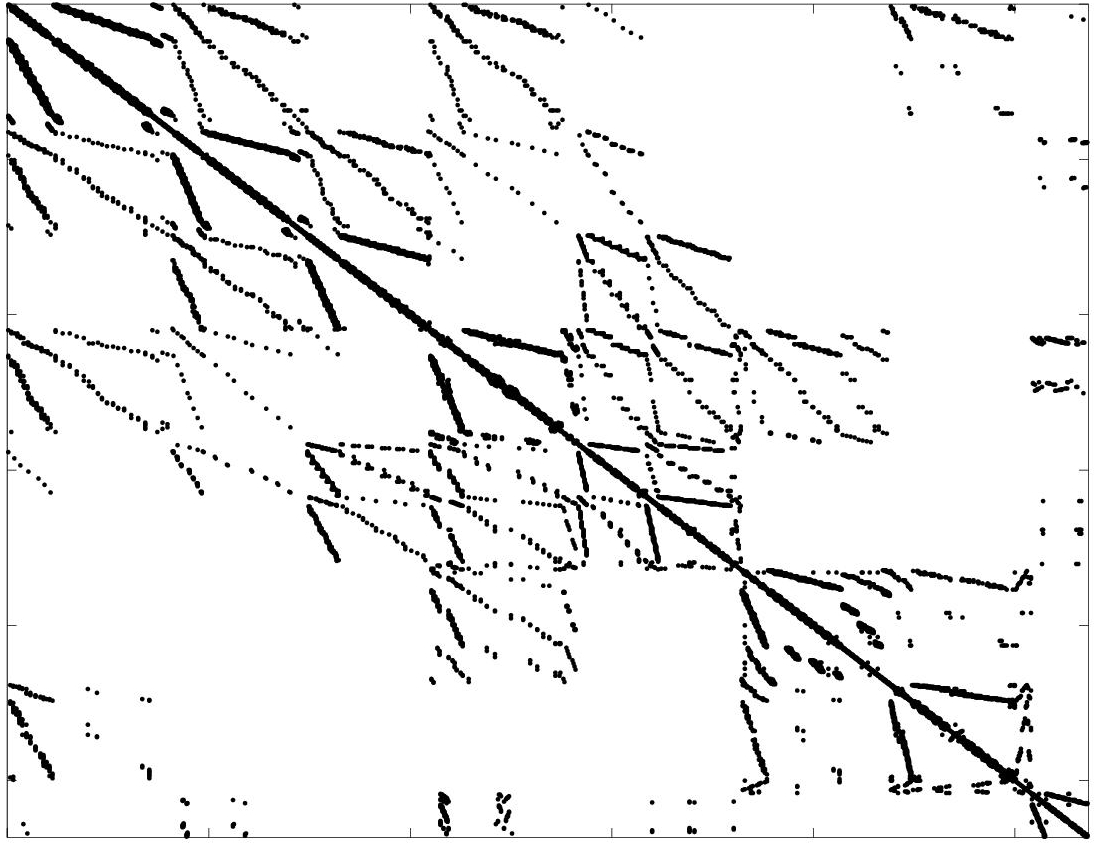
\includegraphics[scale=.23]{can_1072_1072_12444.jpg} \label{fig:sp_1}}
  %\hspace{+1mm}
	\subfloat[]{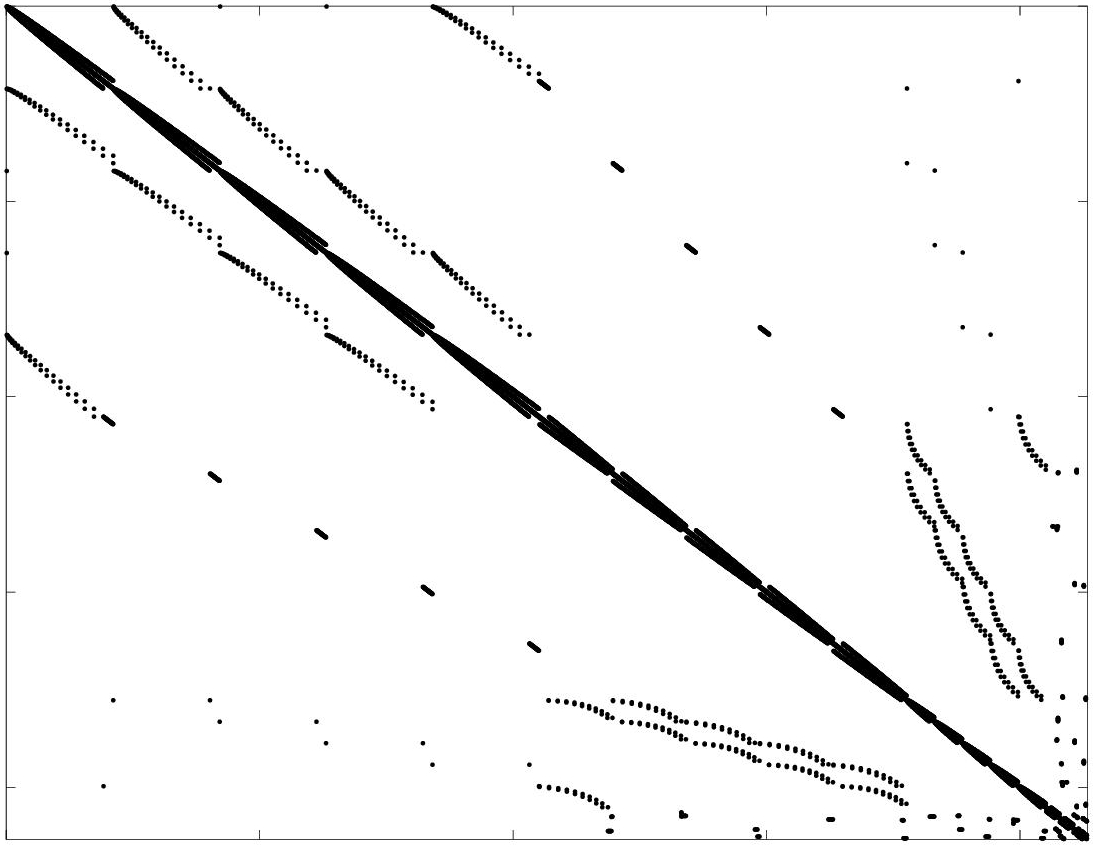
\includegraphics[scale=.23]{blackhole_2132_14872.jpg} \label{fig:sp_2}
	}
  %\hspace{-1mm}
	\subfloat[]{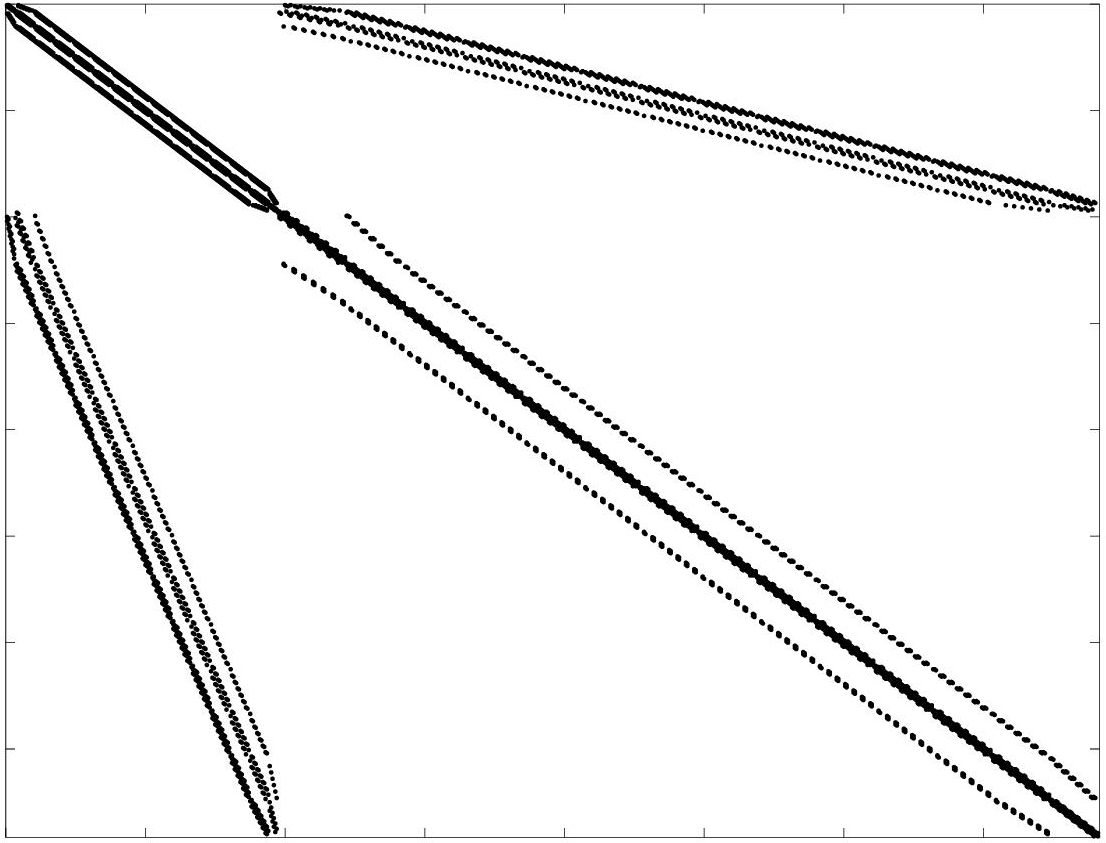
\includegraphics[scale=.23]{bfw782b_782_5982.jpg} \label{fig:sp_3}
	}
	\caption[Samples of sparse matrices.]{Samples of sparse matrices resulting from different \gls{acr:fem} application areas. The matrices are obtained from the Matrix Market online repository \cite{bib:matrixMarket} and plotted using Octave \cite{bib:octave2012}. The application areas are: \protect\subref*{fig:sp_1} Aircraft structure, matrix name: ``can 1027'' $N=1027$ $\gls{acr:nnz}=12444$. \protect\subref*{fig:sp_2} Structural engineering, matrix name: ``blackhole'' $N=2132$ $\gls{acr:nnz}=14872$.  \protect\subref*{fig:sp_3} Waveguide, matrix name: ``bfw782b'' $N=782$ $\gls{acr:nnz}=5982$.}
	\label{fig:sparseMat}
\end{figure}

Sparse data-structures mainly store the non-zero elements of the matrix and their locations based on their row and column indices.
However, the arrangement of the data-structure will need to support two key objectives.
The first objective is to minimize the overall data-structure size by reducing the overhead data, such as pointers, indices, and zero paddings if needed.
The second objective is to organize the data-structure in such a way to hide the memory access latencies and improve the memory bandwidth utilization for basic sparse operations such as the \gls{acr:smvm}.
Obtaining good performance for sparse solvers on \gls{acr:hpc} platforms usually requires balancing the trade-offs from these two objectives.
At the present time however, memory chips can be provided at commodity prices while memory bandwidth (connectivity with the CPU) remains limited; as a result, the second objective will usually have more impact on performance than the first one.

Examples of commonly used sparse data-structure formats are the \gls{acr:cc}, the \gls{acr:csr}, the \gls{acr:csc}, and the \gls{acr:jd}.
In the \gls{acr:cc} format, each non-zero is stored along with its row and column indices; hence, the \gls{acr:cc} format is known to be the simplest and most flexible of all formats.
The \gls{acr:cc} format however requires the largest overhead to store.
The \gls{acr:csr} format, on the other hand, requires less memory and performs relatively better for sparse operations such as the \gls{acr:smvm}, hence it became one of the most popular formats.
\figRef{fig:sparseFormats} illustrates a simple example of the \gls{acr:cc} and the \gls{acr:csr} formats.

\begin{figure}[h]
	\centering
	\subfloat[]{%
	\begin{minipage}[c]{0.5\textwidth}%
		\[
		A=\left[\begin{array}{ccccc}
			1. & 0. & 6. & 0. & 0.\\
			0. & 2. & 0. & 0. & 0.\\
			6. & 0. & 3. & 0. & 0.\\
			0. & 0. & 0. & 4. & 8.\\
			0. & 0. & 0. & 8. & 5.
		\end{array}\right]
		\]
	\end{minipage}%
	\label{fig:ssp}}
	\vfill
	\subfloat[]{%
	\begin{minipage}[c]{\textwidth}%
		\centering
		\begin{tabular}{l|lllllllll|}
			\cline{2-10} 
			$Ae$         & 1. & 2. & 3. & 4. & 5. & 6. & 6. & 8. & 8.\tabularnewline
			\cline{2-10}
			\multicolumn{10}{l}{}\\[-2ex]
			\cline{2-10}
			$Ri$         & 1  & 2  & 3  & 4  & 5  & 1  & 3  & 4  & 5\tabularnewline
			\cline{2-10}
			\multicolumn{10}{l}{}\\[-2ex]
			\cline{2-10}
			$Ci$         & 1  & 2  & 3  & 4  & 5  & 3  & 1  & 5  & 4\tabularnewline
			\cline{2-10} 
		\end{tabular}
	\end{minipage}
	\label{fig:cc}
	}
	\vfill
	\subfloat[]{%
	\begin{minipage}[c]{\textwidth}%
		\centering
		\begin{tabular}{l|lllllllll|}
			\cline{2-10} 
			$Ae$         & 1. & 6. & 2. & 6. & 3. & 4.                      & 8. & 8. & 5.\tabularnewline
			\cline{2-10}
			\multicolumn{10}{l}{}\\[-2ex]
			\cline{2-10}
			$Ri$         & 1  & 3  & 2  & 1  & 3  & 4                       & 5  & 4  & 5\tabularnewline
			\cline{2-10}
			\multicolumn{10}{l}{}\\[-2ex]
			\cline{2-7}
			$Rp$         & 1  & 3  & 4  & 6  & 8  & \multicolumn{1}{l|}{10} &    &    & \multicolumn{1}{l}{}\tabularnewline
			\cline{2-7} 
		\end{tabular}
	\end{minipage}
	\label{fig:csr}
	}
	\caption[Examples of two sparse data-structure formats.]{Examples of two sparse data-structure formats where $Ae$ is the elements list of the matrix $A$, $Ri$ is the element row index list, $Ci$ is the element column index list, and $Rp$ is the row start index list. \protect\subref*{fig:ssp}~The sparse matrix. \protect\subref*{fig:cc}~The \gls{acr:cc} format. \protect\subref*{fig:csr}~The \gls{acr:csr} format.}
	\label{fig:sparseFormats}
\end{figure}


\subsection{Sparse Linear Solvers}

Sparse linear solvers mainly fall into two categories, sparse direct solvers and sparse iterative solvers.
Sparse direct solvers perform some type of LU or Cholesky factorization while reducing the effect of fill-ins.
Fill-in is a side-effect of direct sparse solvers that occurs from the factorization process by introducing non-zeros in locations that were zeros in the original sparse matrix.
The effect of fill-in can negatively impact the CPU's performance by progressively increasing the memory and the computational requirements.
Widely used open-source libraries for sparse direct solvers include UMFPACK \cite{bib:UMFPACKDavis2004,bib:Davis2004CPS}, SuperLU \cite{bib:SuperLU,bib:SuperLUUG}, and MUMPS \cite{bib:MUMPS}.
Specialized matrix reordering algorithms such as the \gls{acr:md} \cite{bib:George1989TEOTMDOA} reordering and the \gls{acr:nd} \cite{bib:George1973NestedDisssection} reordering can help in reducing the amount of fill-ins.
Sparse direct solvers can be particularly efficient for problems requiring multiple solutions for different right hand side vectors (different $b$ vectors in \eqnRef{eqn:aub}), since only forward-backward substitution is needed to be applied on each right hand side after the first solve.
Due to fill-in that substantially increases in 3D problems, the performance of sparse direct solvers is particularly worse than iterative solvers.
A sparse Cholesky factorization would require $\bigo{N^2}$ operations and $\bigo{N^{4/3}}$ memory for discretized 3D Poisson's problems \cite[p.~278]{bib:Demmel1997anla}.
Therefore, iterative solvers are more popular in \gls{acr:hpc} applications because they scale more efficiently for larger problems in terms of both memory requirement and execution time.
In fact, certain iterative solvers can achieve the optimal computational time of $\bigo{N}$ and the optimal memory space of $\bigo{N}$ such as multigrid solvers or preconditioners.
Henceforth, our focus in this work will be directed towards iterative solvers.
In particular, we consider applications that result in linear systems with $A$ being \gls{acr:spd}.
Such a property is commonly present in linear systems generated by a wide range of \gls{acr:fem} applications.
Also, certain methods developed for \gls{acr:spd} matrices can be generalize to non-symmetric positive definite matrices such as the \gls{acr:bicg} method or, for more general definite systems, the \gls{acr:gmres} method.
However, the two methods, the \gls{acr:bicg} and the \gls{acr:gmres}, are considered specializations of a wider class of solvers known as the \acrfullpl{acr:ksm}.


Two widely used iterative solvers are the \gls{acr:cg} method and the multigrid scheme.
Extensive literature is devoted to these methods since their early conception.
Recent references that introduce the theory, as well as various implementation approaches, include \cite{bib:Saad2003IMFSLS2E,bib:Demmel1997anla,bib:Demmel1994Templates,bib:Golub1996MC,bib:Briggs2000AMT,bib:Trottenberg2001M,bib:Shewchuk1994ICG}.
The \gls{acr:cg} method in particular, which was first introduced in 1950, only found wide use in the early 1970s when the efficiency of the method was vastly improved by the introduction of preconditioning \cite{bib:Golub1989SHC}.  
In the following sections we provide a brief overview of these methods.


\subsection{The Preconditioned Conjugate Gradient}
\label{sec:pcg}

The \gls{acr:cg} algorithm, applicable when $A$ is \gls{acr:spd}, is a special case of a more general class of algorithms referred to as \glspl{acr:ksm}.
In such algorithms, the sequence of approximate solutions $u_m$ are taken from an evolving subspace spanned by vectors resulting from repeatedly applying the matrix $A$ on the initial residual $r_0 = b-Au_0$.
Such a space is referred to as the Krylov-subspace and is denoted as $\mathcal{K}_m = \OpN{span}\{r_0,Ar_0,A^2r_0,\cdots,A^{m-1}r_0\}$.
The \gls{acr:cg} algorithm can be viewed as a search direction algorithm that obtains $A$-orthogonal (conjugate) directions from the search space $\mathcal{K}_m$ in order to minimize the following quadratic:
\begin{equation}
	\mathcal{Q}(u) = \frac{1}{2}u^TAu-b^Tu + c \label{eqn:quad}
\end{equation}
where $c$ is a constant.
It can be shown that the optimum point, ($u_\star$), satisfies the gradient of $\mathcal{Q}$ such that $\nabla\mathcal{Q}\mid_{u=u_\star} = Au_\star - b = 0$.
Using the residuals as the conjugating vectors in the Gram-Schmidt orthogonalization process results in the elaborate \gls{acr:cg} algorithm.
A key advantage of using conjugated directions is that in each iteration the error is not only being minimized in the current search space, but rather in all subspaces of the search space.
As a result, the \gls{acr:cg} algorithm theoretically reaches the optimal solution in $N$ iterations.
In practice however, the \gls{acr:cg} algorithm converges in less than $N$ iterations; for example, in Poisson's problems the convergence is upper-bounded by $\bigo{N^{3/2}}$ for 2D and $\bigo{N^{4/3}}$ for 3D \cite{bib:Shewchuk1994ICG}.
Preconditioning considerably improves the convergence of \gls{acr:cg} by improving the characteristics of the matrix $A$ at the expense of an additional computational cost per each iteration.
In \gls{acr:pcg}, a \gls{acr:spd} preconditioner matrix ($M$) is selected to approximate $A$ such that the residuals can be made $M^{-1}$-orthogonal.
Clearly for the preconditioning process to be efficient, $M$ must be considerably easier to solve than $A$.
The \gls{acr:pcg} algorithm pseudocode is listed in \algRef{alg:pcg}.  
The key computational kernels in the \gls{acr:pcg} algorithm are the \gls{acr:smvm}, shown in Line~\ref{alg:smvmLine}, and the preconditioner solve step, shown in Line~\ref{alg:precLine}.

\begin{algorithm}
  %\centering
	\begin{algorithmic}[1]
		\STATE \textbf{initialize:}
		\STATE ~ ~$r_0 = b - Au_0$
		\STATE ~ ~\text{solve: } $M z_0  = r_0$
		\STATE ~ ~$d_0 = z_0$
		\REPEAT[Iterate $t=1,2,\cdots$]
		\STATE $\theta_t = z_t^Tr_t$
		\STATE $v_t = Ad_t$ \label{alg:smvmLine}
		\STATE $\rho_t = \frac{\theta}{d_t^Tv_t}$
		\STATE $u_{t+1} = u_t + \rho_t d_t$
		\STATE $r_{t+1} = r_t - \rho_t v_t$
		\STATE \text{solve: } $z_{t+1} M = r_{t+1}$ \label{alg:precLine}
		\STATE $\theta_{t+1} = z_{t+1}^Tr_{t+1}$
		\STATE $ \gamma_t = \frac{\theta_{t+1}}{\theta_t}$
		\STATE $d_{t+1} = z_{t+1} + \gamma_t d_t $
		\UNTIL{convergence: $r_{t+1}$ sufficiently small}
		\STATE \textit{Output:} $u_{t+1}$
	\end{algorithmic}
	\caption[The \acrshort{acr:pcg} algorithm.]{The \glsfirst{acr:pcg} algorithm.}
	\label{alg:pcg}
\end{algorithm}



\subsection{The Multigrid Scheme}
\label{sec:RMG}

Multigrid accelerated solvers \cite{bib:Briggs2000AMT,bib:Trottenberg2001M,bib:multigridZhu2006} are among the fastest known algorithms to obtain solutions to linear systems of equations resulting from the \gls{acr:fem}.
The performance of multigrid can, in practice, be shown to be independent of the size of the finest discretization of the domain \cite{bib:Briggs2000AMT,bib:Trottenberg2001M}, attaining the optimal complexity of $\bigo{N}$ for both computation and memory.
In this section we present the general principles behind the multigrid scheme.


Multigrid schemes are based on creating different levels of approximations to a problem so as to obtain progressively lower complexities, or lower number of unknowns, on each sub-level.
An approximate solution can be obtained very quickly on the lowest complexity level.
The approximate solution is then transferred progressively to the problem's actual level of accuracy.
This process is repeated iteratively in the hopes of speeding-up the overall computation time.
The problem levels have to be related according to a criterion, otherwise the approximated solution can not be relayed across the adjacent levels.
In the case of \gls{acr:fem} applications, different problem levels can be created by performing nested mesh refinement, referred to as hierarchical mesh refinement.
Such hierarchical meshing schemes are obtained by splitting each mesh element into smaller elements.
Multigrid schemes using hierarchical meshes are referred to as the \gls{acr:gmg}.
An example of an \gls{acr:fem} library that uses \gls{acr:gmg} is the open-source library \dealName{} \cite{bib:dealii2007}.
Alternatively, different levels of problem operators can be generated using algebraic operations on the matrix $A$, such multigrid schemes are referred to as the \gls{acr:amg}.


The key advantage of \gls{acr:amg} schemes is that they are designed to be used as black-box solvers where all that is needed from the underlying \gls{acr:pde} problem is the sparse linear system \eqnRef{eqn:aub}.
An example of a solver library that uses \gls{acr:amg} is the open-source library BoomerAMG~\cite{bib:boomerAMG}.
\Gls{acr:amg} solvers are used in frameworks where the sparse matrix $A$ is assembled once on the finest level.
However, an \gls{acr:amg} solver requires a number of global sparse algebraic operations as well as processing a number of sparse data-structures for each generated level operator.
While \gls{acr:gmg}, on the other hand, provides the potential of implementing matrix free operations.
In addition, \gls{acr:gmg} performs considerably better because it can better utilize the inherent problem structure in the hierarchical \gls{acr:fem} mesh to lower the computational complexity.
Therefore, it is advisable to use \gls{acr:amg} only when it is impossible, or difficult, to setup \gls{acr:gmg}.
Hence, the choice weather to use \gls{acr:amg} or \gls{acr:gmg} is more application dependent than it is performance dependent.
Our work, described in \chpRef{chp:FMGaBP}, utilizes \gls{acr:gmg} schemes to accelerate a parallel formulation of the \gls{acr:fem} problem.


To illustrate the key formulations behind the multigrid solvers, we provide here a brief overview of the two-grid correction scheme.
Given an initial discretization for a continuous bounded domain $\Omega$, refereed to as a coarse mesh $\Omega^H$, then the mesh is refined further by element splitting schemes into a finer mesh $\Omega^h$.
This refinement scheme is illustrated in \figRef{fig:LSM}.
The multigrid correction scheme is based on the simple reformulation of the linear system $Au=b$ into the residual-correction scheme.
Given an exact solution $u_\star$ and an initial approximation $\tilde{u}$, then the correction $z$ can be stated as:
\begin{equation}
	z = u_\star - \tilde{u}. \label{eqn:crr}
\end{equation}
We start by finding the residual:
\begin{equation}
	r = b - A\tilde{u}, \label{eqn:res}
\end{equation}
then the solution to the system $Au=b$ can alternatively be obtained by solving for the correction as:
\begin{equation}
	Az=r, \label{eqn:azr}
\end{equation}
with the initial guess $z=0$. 
The obtained correction $z$ is then added to the initial approximation $\tilde{u}$ to obtain the solution as:
\begin{equation}
	u_\star = z + \tilde{u}.
\end{equation}

The residual-correction reformulation has no computational advantage in itself; however, this reformulation is converted into an iterative process by multigrid.
Using multigrid, the correction in \eqnRef{eqn:azr} is rather computed on a coarse grid (smaller version of $A$) which is then used to compute an improved initial approximation for the fine grid.
We expect an overall computational advantage, since working on the coarse grid is cheaper than working on the fine grid.

\begin{figure}
	\centering
	\subfloat[]{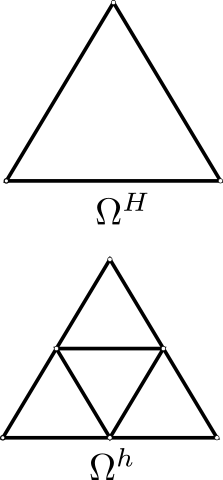
\includegraphics[scale=.3]{tri_split} \label{fig:split}}
  %\hspace{+1mm}
	\subfloat[]{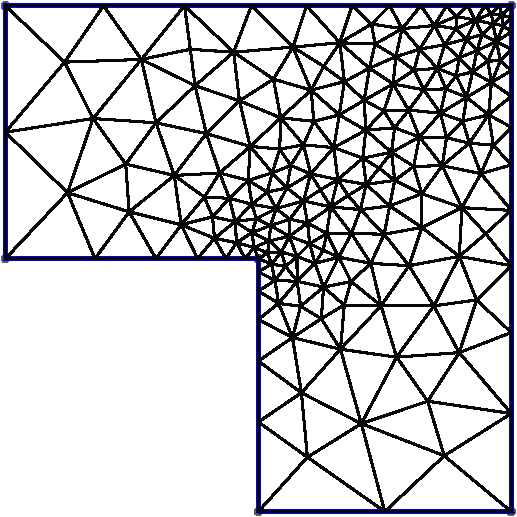
\includegraphics[scale=.5]{LSC} \label{fig:LSC}
	}
  %\hspace{-1mm}
	\subfloat[]{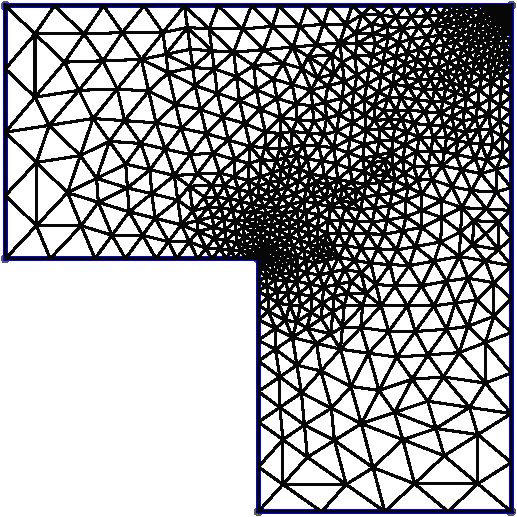
\includegraphics[scale=.5]{LSF} \label{fig:LSF}
	}
	\caption[Mesh refinement by splitting.]{\protect\subref*{fig:split} Mesh refinement by splitting each triangle in mesh $\Omega^H$ into four geometrically similar sub-triangles to produce a finer mesh $\Omega^h$. \protect\subref*{fig:LSC} Sample coarse irregular mesh.  \protect\subref*{fig:LSF} The refined mesh by splitting.}
	\label{fig:LSM}
\end{figure}

We redefine the linear system in \eqnRef{eqn:aub} as $A^h u^h = b^h$; where the superscript $h$ represents the linear system of the fine mesh $\Omega^h$. 
If the superscript $H$ is used, then the system represents the coarse mesh.
The listing in \algRef{alg:2VMG} shows the detailed operations of the two-grid V-cycle multigrid.
A single iteration of the algorithm is refereed to as a V-cycle which reflects the behavior of the algorithm in transferring approximations from fine to coarse grids and then back from coarse to fine grids.
Other key components of the algorithm are the restriction and prolongation operators.
The restriction operator $\mathcal{R}_{h}^{H}$ acts on the residual from the fine grid by mapping it from the fine grid onto the coarse grid using restriction.
On the other hand, the prolongation operator $\mathcal{I}_{H}^h$ acts on the correction from the coarse grid by mapping it onto the fine grid using interpolation.
Since restriction and prolongation operators act on the global residual and correction vectors, they are in fact some form of global sparse operations.
However, in certain applications, such as the \gls{acr:fdm}, these operators can be performed on a point-by-point basis.
In linear transfer operations, the dimensions of $\mathcal{R}$ is given by $(N_H\times N_h)$ where $N_H$ is the number of unknowns in the coarse grid, while $N_h$ is the number of unknowns in the fine grid.
On the other hand, the dimension of $\mathcal{I}$ is $(N_h\times N_H)$.
This residual-correction scheme is also effective in progressively minimizing the error added due to both the restriction and the prolongation operations as the approximate solution on the fine grid approaches the exact solution.
In addition, since the problem has a unique solution, it can be shown that the whole multigrid process can be viewed as a fixed-point process for the exact solution on the fine grid.

\begin{algorithm}[t]
  %\centering
  %\begin{framed}
	\begin{algorithmic}[1]
		\STATE Set initial guess $z^{h}_0=0$
		\REPEAT[V-cycle iterate]
		\STATE Obtain the approximate solution $\tilde{u}^{h}_0$ from $A^h u^h = b^h$ on the fine grid $\Omega^h$ using $v_1$ iterates (pre-smoothing) of a relaxation algorithm with initial guess $z^{h}_0$.\label{alg:fg}
		\STATE Compute the residual $r^h = b^h - A^h \tilde{u}^{h}_0$.
		\STATE Restrict the residual on the coarse grid $\Omega^H$ using $r^H = \mathcal{R}_{h}^{H} r^h$, where $\mathcal{R}_{h}^{H}$ is a fine-to-coarse restriction operator.
		\STATE Obtain the coarse grid correction $\tilde{e}^H$ by solving $A^H e^H = r^H$ with initial guess $e^H = 0$.\label{alg:crr}
		\STATE Compute $z^{h}_1 = \tilde{u}^{h}_0 + \mathcal{I}_{H}^h \tilde{e}^H$, where $\mathcal{I}_{H}^h$ is a coarse-to-fine prolongation operator.
		\STATE Obtain the approximate solution $\tilde{u}^{h}_1$ from $A^h u^h = b^h$ using $v_2$ iterates (post-smoothing) with initial guess $z^{h}_1$.
		\STATE Set new initial guess $z^{h}_0 = \tilde{u}^{h}_1$.
		\UNTIL{Convergence on fine grid.}
	\end{algorithmic}
  %\end{framed}
	\caption{The two-grid V-cycle multigrid process.}
	\label{alg:2VMG}
\end{algorithm}

To elaborate more on the behavior of the restriction and the prolongation operations, we consider a simple example using a 2D quadrilateral mesh shown in \figRef{fig:grid_trans_a}
The coarse mesh contains only one quadrilateral element, while the fine mesh contains four refined quadrilateral elements by splitting the coarse grid element evenly.
The nodal numbers on the diagram reflect global numbering of the indices.
Similarly as indicated in \figRef{fig:grid_trans_b}, a triangular mesh can be refined by splitting a triangular element into four geometrically similar child triangles.
This splitting is performed by connecting nodes inserted at the mid point of each edge in the parent triangle.
\begin{figure}[t]
	\centering
	\subfloat[]{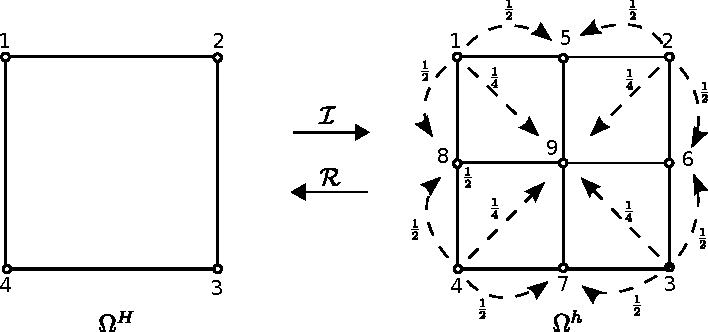
\includegraphics[scale=.8]{grid_trans_a} \label{fig:grid_trans_a}}
	\vfill
	\subfloat[]{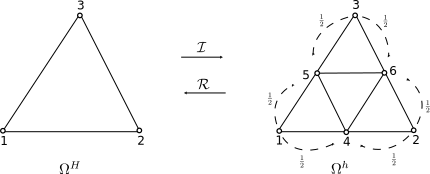
\includegraphics[scale=.8]{grid_trans_b} \label{fig:grid_trans_b}}
	\caption[Multigrid transfer operations.]{Grid transfer operations between: \protect\subref*{fig:grid_trans_a} two 2D quadrilateral meshes and  \protect\subref*{fig:grid_trans_b} 2D triangular meshes. The fractions indicated on the fine meshes represent nodal weightings for the case of linear interpolation.}
	\label{fig:grid_trans}
\end{figure}


The prolongation operator $\mathcal{I}_H^h$ can be defined using linear interpolation.
In linear interpolation, the correction values of the fine grid nodes, which do not overlap the coarse grid nodes, are obtained by averaging the surrounding nodes from the coarse grid.
The overlapping nodes on the fine grid can retain the same correction values from the coarse grid.
Hence the operator $\mathcal{I}_H^h$ matrix can be defined as:
\begin{equation}
	\mathcal{I}_{H}^{h}=\left[\begin{array}{cccc}
		1 & 0 & 0 & 0\\
		0 & 1 & 0 & 0\\
		0 & 0 & 1 & 0\\
		0 & 0 & 0 & 1\\
		\frac{1}{2} & \frac{1}{2} & 0 & 0\\
		0 & \frac{1}{2} & \frac{1}{2} & 0\\
		0 & 0 & \frac{1}{2} & \frac{1}{2}\\
		\frac{1}{2} & 0 & 0 & \frac{1}{2}\\
		\frac{1}{4} & \frac{1}{4} & \frac{1}{4} & \frac{1}{4}
	\end{array}\right].\label{eqn:mgIntr}
\end{equation}
The restriction operator $\mathcal{R}_{h}^{H}$ is defined by linear injection, that is by assigning the residual values of the coarse grid nodes the same restriction values of the overlapping fine grid nodes.
Other forms of averaging schemes can also be employed in certain cases.
Using injection, the operator $\mathcal{R}_{h}^{H}$ matrix can be defined as:
\begin{equation}
	\mathcal{R}_{h}^{H}=\left[
	\begin{array}{cc}
		\begin{array}{cccc}
			1 & 0 & 0 & 0\\
			0 & 1 & 0 & 0\\
			0 & 0 & 1 & 0\\
			0 & 0 & 0 & 1
		\end{array} &
		\left[0\right]
	\end{array}
	\right]. \label{eqn:mgInj}
\end{equation}
However, in certain multigrid applications, $\mathcal{I}_H^h$ can simply be defined by enforcing the condition:
\begin{equation}
	\mathcal{R}_{h}^{H} = a \left(\mathcal{I}_{H}^{h} \right)^T \,\,\textrm{and } a\in \mathbb{R}^+,
\end{equation}
where $a$ is a constant.


In practice, the two-grid V-cycle process is generalized to a recursive multigrid process by restricting the residual to lower levels of consecutive coarser grids.
Once the coarsest grid is reached, the correction $e^{H}$ is obtained using a direct solver.
The correction is then prolongated progressively to higher levels of finer grids.
On each level down the V-cycle, $v_1$ number of iterations are executed, while $v_2$ number of iterations are executed on each level up the V-cycle.


Multigrid techniques can vary widely by using different relaxation algorithms with different approximation properties, the approach of generating coarse grids operators, and the types of grid transfer operations that involve restriction and prolongation \cite{bib:Briggs2000AMT,bib:Trottenberg2001M}.
Hence, the performance of any multigrid scheme can strongly depend on these variations.
In general, multigrid accelerated algorithms show much better scalability and parallel efficiency than their non-multigrid counterparts.
This is particularly evident when using multigrid as a preconditioner for the \gls{acr:cg} method.
In \cite[p.~284]{bib:Trottenberg2001M}, it was found that the complexity of solving Poisson's equation using \gls{acr:icpcg} was $\bigo{N^{5/4}}$ for 2D and $\bigo{N^{9/8}}$ for 3D; whereas, the \gls{acr:mgpcg} can achieve approximately $\bigo{N}$ complexity which is an optimal result \cite{bib:KettlerACMGCG}.
Trottenberg et al. \cite[p.~278]{bib:Trottenberg2001M} presents \gls{acr:mgpcg} as a multigrid accelerated by a Krylov-subspace method by recombining successive approximations in a way to minimize the residual using a Gram-Schmidt orthonormalization process.
In addition, the \gls{acr:mgpcg} has been shown to exhibit a robust convergence on domains with geometric singularities.
Due to the optimal performance expectation of \gls{acr:mgpcg}, we will use it as a performance comparison to illustrate the advantages of the new \gls{acr:fmgabp} algorithm, presented later in \chpRef{chp:FMGaBP}, using test cases of Poisson's problems on domains with geometric singularities, or non-convex domains, such as the L-shaped domain shown in \figRef{fig:LSM}. 


\section{The Finite Element Method}
\label{sec:FEMVF}


In this section, a brief overview of the \glsfirst{acr:fem} is presented.
The \gls{acr:fem} is a widely used numerical technique for obtaining approximate solutions to \gls{acr:pde} problems.
The \gls{acr:fem} is also a computationally intensive method which can greatly benefit from efficient execution on parallel platforms.
After introducing the \gls{acr:fem}, we will illustrate its computational challenges and elaborate on the shortcomings of conventional schemes which attempt to accelerate the \gls{acr:fem} computations.


The Helmholtz equation is a particular class of \glspl{acr:pde} that addresses many of the electromagnetic formulations resulting from Maxwell's equations.
The \gls{acr:fem} is a key method that is commonly used to obtain numerical solutions to the Helmhotz equation.
The \gls{acr:fem} employs two types of formulations for approximating the \gls{acr:pde} problem, the Ritz formulation and the Galerkin formulation.
To obtain further details on these two methods including derivations for a wider set of electromagnetic applications, the reader can refer to Silvester et al.~\cite{bib:Silvester1996FEEE} or Jin~\cite{bib:Jin2002TFEMIE}.
Our overview here presents only the key formulations for obtaining approximate solutions to the Helmholtz equation using the \gls{acr:fem} Ritz formulation.
We chose the Ritz formulation since it is based on a variational formulation of the underlying Helmholtz \gls{acr:pde}.
More importantly, the \gls{acr:fem} variational formulation provides critical insights that facilitates the derivation of our highly parallel \gls{acr:fgabp} method, later addressed in \chpRef{chp:FGaBP}.
The general scalar Helmholtz equation is stated as follows:
\begin{equation}
	\nabla\cdot\left(p\nabla u\right)+k^2 q u=g
	\label{eqn:bvp}
\end{equation}
where $u$ is the unknown field defined on the bounded domain $\Omega$; $p$ and $q$ are known parameters associated with the material properties of the domain; $k^2$ is a constant quantity independent of position.
Lapace, and Poisson \gls{acr:pde} equations are special cases of~\eqnRef{eqn:bvp}.
For example, the familiar Laplace's equation
\begin{equation}
	\nabla^2 u = 0
	\label{eqn:lap}
\end{equation}
results by setting $p=1$, $q=0$ and $g=0$.
Whereas introducing material properties $\epsilon = p(x,y,z)$ and allowing sources $g=-\rho(x,y,z)$, we obtain the more general Poisson's equation
\begin{equation}
	\nabla\cdot\left(\epsilon\nabla u\right) = -\rho.
	\label{eqn:pss}
\end{equation}


The equations \eqnRef{eqn:bvp}, \eqnRef{eqn:lap} and \eqnRef{eqn:pss} are also referred to as \glspl{acr:bvp} because they can only be uniquely solved by defining conditions on the domain's boundary ($\partial \Omega$).
These boundary conditions are generally stated as follows:
\begin{align}
	u & =u_{0}\mbox{ on }\partial D \label{eqn:dbc}\\
	\nabla u\cdot\hat{n}+au & =v_{0}\mbox{ on }\partial C \label{eqn:cbc}
\end{align}
where $\partial D$ and $\partial C$ are boundary segments such that $\partial D \cup \partial C = \partial \Omega$; the parameters $a$, $u_0$, and $v_0$ are known parameters associated with the properties of the boundary; and the vector $\hat{n}$ is the outward normal unit vector of the boundary.
The condition in \eqnRef{eqn:dbc} is commonly referred to as the Dirichlet boundary condition.
When $a=0$, \eqnRef{eqn:cbc} is referred to as the Neumann boundary condition; however, with the added condition $v_0=0$ it is termed the homogeneous Neumann boundary condition.


Considering scalar potential problems with lossless media and general inhomogeneous boundary conditions as stated in \eqnRef{eqn:dbc} and \eqnRef{eqn:cbc}, the solution to the scalar Helmholtz equation can be obtained by rendering stationary the following functional:
\begin{align}
	\mathcal{F}(U) & =\frac{1}{2}\int_{\Omega}\left(p\nabla U\cdot\nabla U-k^2 qU^{2}+2gU\right)\,\mathrm{d}\Omega + \frac{1}{2}\int_{\partial C} a p U^2 \mathrm{d}\Gamma - \int_{\partial C}pUv_0 \mathrm{d}\Gamma \label{eqn:globalFunc}
\end{align}
where $U$ is an admissible approximating function space of the unknown field $u$ and $\Gamma$ is a boundary segment.
While the functional $\mathcal{F}$ provides a means of finding the solution to the Helmholtz equation by avoiding the original \gls{acr:bvp}, it does not, however, provide an indication on how to chose the admissible functions $U$.
This is where the \gls{acr:fem} comes into play.



\subsection{The FEM Solution}
\label{sec:FEMSol}

The \gls{acr:fem} provides a rigorous method for obtaining an approximate solution to the \gls{acr:bvp} through two main steps.
The first step is the discretization of the continuous domain $\Omega$ into finite subdivisions referred to as finite elements.
The second step is choosing appropriate interpolation functions that setup the function space $U$ while guaranteeing its continuity across the discretized elements within the domain $\Omega$.
Different approaches of the \gls{acr:fem} can vary widely based on the details of how the above steps are carried out; however, we will highlight here the key concepts behind these steps.


The process of discretization, where the domain is subdivided into connected finite elements of a particular shape, is commonly referred to as meshing.
The finite elements can be of any geometrical shape as long as they are connected through their vertices.
Most commonly used geometrical shapes are triangles or quadrilaterals for 2D domains and tetrahedrons or hexahedrons for 3D domains.
Figure~\ref{fig:disc_domain} shows an example 2D domain discretized with four connected triangular elements.


\begin{figure}
	\centering
	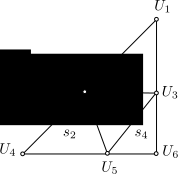
\includegraphics[scale=1.0]{disc_domain}
	\caption{A sample 2D domain discretized with four triangular elements of the first order.}
	\label{fig:disc_domain}
\end{figure}


Two types of meshes are commonly used which are referred to structured meshes and unstructured meshes.
The vertices in a structured mesh lie on grid lines that pass uninterrupted throughout the domain.
As a result, locality information, such as neighboring vertices or edges, can be directly computed from the nodes' indices.
This offers a critical advantage in reducing the overall CPU's memory communication overhead.
However, structured meshes do not adapt well to arbitrary geometries.
Unstructured meshes, on the other hand, place vertices on arbitrary locations in the domain.
As a result, the CPU will require more memory communication overhead in order to process an unstructured mesh.
The key advantage of unstructured meshes though, is that they can better adapt to arbitrary geometries than structured meshes.
In addition, unstructured meshes can allow for increased refinement on local patches situated in interesting domain locations while maintaining coarser patches in other areas.
This results in an improved overall solution accuracy with a lower computational cost.
\figRef{fig:meshTypes} illustrates the two types of meshes.
It is important to note here that, the \gls{acr:fgabp} algorithm does not depend on the type of mesh used; as will later be shown, the \gls{acr:fgabp} was implemented and verified to work with both structured and unstructured meshes.


\begin{figure}
	\centering{
	\subfloat[]{
	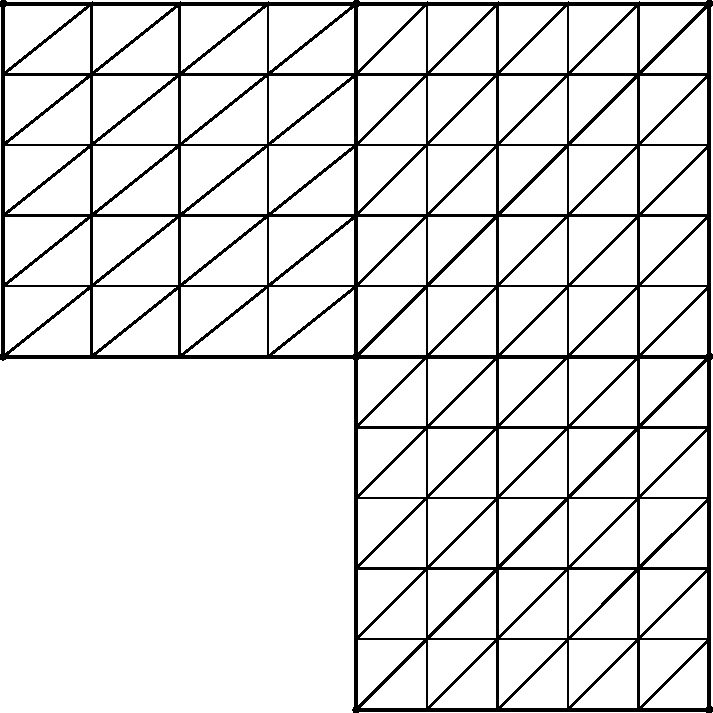
\includegraphics[scale=0.4]{L_shaped_str} \label{fig:strMesh}
	}
  %\hspace{+1mm}
	\subfloat[]{
	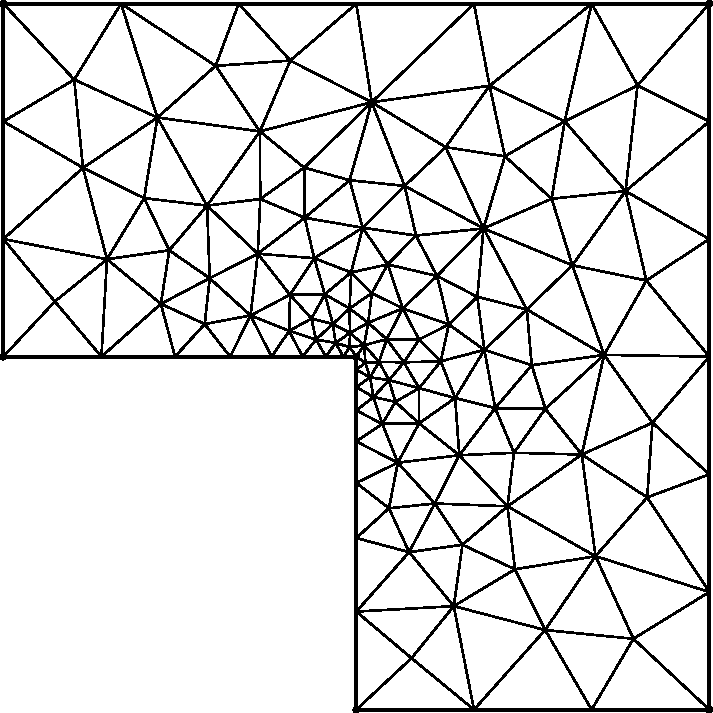
\includegraphics[scale=0.4]{L_shaped_unstr} \label{fig:unstrMesh}
	}
	}
	\caption[Structured and unstructured meshes.]{Structured and unstructured meshes of the L-shaped domain.  \protect\subref*{fig:strMesh} The structured mesh.  \protect\subref*{fig:unstrMesh}~The unstructured mesh. The unstructured mesh provides more refinement at areas of more interest in the domain such as the reentrant corner of the L-shaped region.}
	\label{fig:meshTypes}
\end{figure}

The second step in the \gls{acr:fem} process involves choosing the interpolation polynomials, or as alternatively known the basis functions, in order to approximate the unknown field $U$ within each of the finite elements.
The interpolation polynomials approximate the unknown field using a discrete set of real-valued parameters spatially positioned along each of the finite elements' vertices or edges.
The number of used parameters identify the polynomial interpolation order; for example, a linear triangular element has three parameters positioned along its vertices whereas a second order triangular element has six parameters positioned along its vertices and edges.
For certain \gls{acr:fem} applications, the quality of the approximation will improve with increasing interpolation order; however, the computational complexity of the \gls{acr:fem} will substantially increase.
An expression of this approximation can generally be stated as follows:
\begin{equation}
	U^s(x,y,z) = \sum_{k=1}^{n} U^s_k P^s_k(x,y,z), \,\,\, \forall s \in \mathcal{S}
	\label{eqn:intrPoly}
\end{equation}
where $s$ is the finite element and $\mathcal{S}$ is the total elements' set spanning the domain $\Omega$; $n$ is the number of local discrete values; and $P$ is the interpolating function.
Note that the subscript $k$ in $U^s_k$ refers to the local element node numbering and not the global node numbering; for example, the element $s_3$ in \figRef{fig:disc_domain} has the globally numbered discrete parameters $U_2$, $U_3$ and $U_5$ of globally unique indices $2$, $3$, and $5$.
Typically in \gls{acr:fem} implementations, a mapping of local to global node numbering needs to be defined.
Another important aspect of interpolation polynomials is that the gradient of the field within each element can also be approximated as:
\begin{equation}
	\nabla U^s(x,y,z) = \sum_{k=1}^{n} U^s_k \nabla P^s_k(x,y,z), \,\,\, \forall s \in \mathcal{S}.
	\label{eqn:intrPolyGrad}
\end{equation}
The specifics of the interpolation functions vary for each \gls{acr:fem} scheme; however, they need to maintain the important property of ensuring the continuity of the $U$ field across the finite element edges.


Since the functional $\mathcal{F}$ in \eqnRef{eqn:globalFunc} can, up to a constant, be viewed as an expression of the total energy stored in the system; therefore, $\mathcal{F}$ can be expressed using the sum of energies of each finite element as follows:
\begin{equation}
	\mathcal{F}(U)=\sum_{s\in\mathcal{S}}\mathcal{F}_{s}(U_{s})
	\label{eqn:discFunc}
\end{equation}
where $\mathcal{S}$ is the total elements' set spanning the domain $\Omega$; $U_s$ is the set of the field discrete unknowns, or degrees of freedom, for the finite element $s$; and $\mathcal{F}_s$ is the energy contribution of $s$.
Therefore by rendering stationary the functional in \eqnRef{eqn:discFunc}, an approximate solution to the Helmholtz equation can be found using the \gls{acr:fem} scheme.
Substituting each of \eqnRef{eqn:intrPoly} and \eqnRef{eqn:intrPolyGrad} into \eqnRef{eqn:globalFunc} and applying a standard derivation process, an expression for the local finite element $\mathcal{F}_s$ can, generally, be formulated as:
\begin{equation}
	\mathcal{F}_s(U_s)=\frac{1}{2} U^T_s M_s U_s -B_s^T U
	\label{eqn:elemtFunc}
\end{equation}
in which we refer to $M_s$ as the element characteristic matrix with dimensions $n$-by-$n$ where $n$ is the number of unknowns per element; and $B_s$ is the element source vector.
It is clear that (\ref{eqn:elemtFunc}) can also incorporate the essential boundary conditions as stated for the \gls{acr:bvp}
when $\mathcal{F}_s$ represents a boundary finite element.


Finally, the \gls{acr:fem} solution is computed by executing three main procedures.
First, all the contributions from all the finite elements in terms of the $M_s$ and the $B_s$ elements are added up into a global and sparse linear system of equations. This process is referred to as the assembly process.
Second, the essential boundary conditions are incorporated into the linear system.
Last, the resulting linear system of the form \eqnRef{eqn:aub} is solved using sparse linear solvers such as the \gls{acr:pcg} method.


\subsection{The FEM Parallel Acceleration Issues}

Conventional \gls{acr:fem} implementations consist of two computationally expensive stages which are the sparse matrix $A$ assembly stage, and the solving stage of the linear system using iterative solvers.
Acceleration of these stages using parallel processing will be limited by memory bandwidth issues due to their dependency on the global sparse data-structure of the matrix $A$.
This scalability issue has been the focus of extensive research lately, because computing manufacturers are increasing their chip's computational throughput by adding more cores rather than frequency scaling due to power limitations at the chip level.
Therefore, in order to obtain good performance from emerging parallel computing architectures, the \gls{acr:fem} computation must scale well with parallel computing.
To better illustrate this issue, we consider the \gls{acr:pcg} method, which is a widely used iterative solver for \gls{acr:fem} applications.
The \gls{acr:pcg} solver requires the execution of a number of global algebraic operations in each iteration such as a \gls{acr:smvm} and a preconditioner solve.
The \gls{acr:smvm} operation, in particular, can strongly impact the overall performance of the \gls{acr:pcg} solver since the memory access time will dominate the computational time due the underlying sparse data-structure.
Considering the \gls{acr:smvm} defined as $y=Ax$, where $A$ is a symmetric sparse matrix while $x$ and $y$ are dense vectors, the operation, in its simplest implementations, can be executed as a number of concurrent vector dot products where each dot product consists of $x$ and a row from $A$.
The result from each dot product updates a single value in the output vector $y$.
The dot products are independent of each other, hence they can be executed in parallel.
While this \gls{acr:smvm} approach seems very intuitive and convenient to implement, it actually results in a very poor performance for key reasons.
The data within each row of $A$ is very sparse and require irregular memory access resulting in very low cache hit rates, which substantially increases the CPU's idle time by waiting for data to arrive, causing the CPU to attain only a small fraction of its peak performance.
Without improving the \gls{acr:smvm} execution on a single CPU, parallelizing the \gls{acr:smvm} will not sustain the potential speedup of the parallel platform.
In fact, this issue is even more pronounced for multicore architectures.
As the number of cores increases, the memory requests consequently increases causing a greater bottleneck for the limited memory bandwidth resources.
This in turn severely limits the parallel scalability of the \gls{acr:smvm} operations as will later be demonstrated in the numerical results of \secRef{sec:FMGaBP_res}.


Many attempts are made to improve the performance of the \gls{acr:smvm}; however, typical implementations of the \gls{acr:smvm} yield poor performance of no more than 10-20\% of the peak CPU throughput \cite{bib:Demmel2007OODMVMOEMP}.
Improving the performance of the \gls{acr:smvm} kernel will require sophisticated programming techniques, code transformations, and data-structures that are tailored to specific CPU, cache and memory architectures \cite{bib:DemmelOSKI}.
Specialized sparse data-structures are devised in order to either exploit the sparsity structure of matrices resulting from specific application areas, or target specific \gls{acr:hpc} architectures.
For example, a recent work in \cite{bib:david2010mabpmt} uses blocking schemes to obtain better performance on multicore architectures.
The work in \cite{bib:elkurdi2007hafem,bib:El-Kurdi2008FAAIOSMMFTFEM} uses stripe-based sparse data-structures to accelerate the \gls{acr:smvm} on \glspl{acr:fpga} using a highly parallel hardware architecture based on a systolic pipeline of processing elements.
The numerical results of these efforts indicate that sustaining good performance for all sparse matrices, even within the same \gls{acr:fem} application area, is nearly impossible.
While there also exist generic and optimized libraries such as Trilinos \cite{bib:Trilinos} and PETSc \cite{bib:PETSc}, which can be used to solve the sparse linear system in parallel, obtaining a sustained performance can prove difficult due to the varying sparsity structure of $A$ resulting from different application areas.
In addition, such libraries do not help with the assembly stage of the \gls{acr:fem}, which in many cases can require more time than the solve stage, such as the case for non-linear applications.
In certain cases, matrix reordering can improve the performance of \gls{acr:smvm} by rearranging its elements so that they are more clustered around the main diagonal.
One of the most popular reordering algorithms to improve the \gls{acr:smvm} performance is the \gls{acr:rcm} algorithm \cite{bib:Cuthill1969RTBOSSM}. 
However, reordering requires considerable overhead processing for large matrices.


Another important sparse operation is the sparse matrix assembly and the buildup of the sparse data-structure based on the matrix specific sparsity pattern.
For specialized data-structures, this operation can be very costly.
Parallelizing the matrix assembly also requires special care.
Since the sparse matrix is a shared data-structure, updating the data-structure from different parallel processes needs to avoid memory collisions when accessing shared elements in the matrix.
One way to overcome this issue is by using element coloring schemes, where adjacent elements are given different colors.
Elements of the same color group can then be assembled concurrently.
While, for certain cases, the assembly needs to be done only once and, therefore, its cost can be tolerated; however, for many cases such as \gls{acr:amg} solvers, adaptive refinement, and non-linear applications, the assembly stage can dominate the solve stage.
This is specially so for non-linear applications requiring non-linear solvers, such as the Newton-Raphson method, where the assembly stage must be repeated each linearizing iteration.
Our numerical results in \secRef{sec:FMGaBP_res} demonstrate that the assembly time was considerably long in comparison with the solve time.

As mentioned earlier, computing manufacturers are increasing the number of CPU cores on a single chip as opposed to frequency scaling in order to keep up with Moore's law \cite{bib:moore1965} of increasing chip transistor density; therefore, new and inherently parallel algorithms need to be devised for the \gls{acr:fem} in order to efficiently scale with these parallel computing trends.
In this work, we take a different approach for \gls{acr:fem} computation by directly minimizing the energy functional (\ref{eqn:discFunc}) using a newly derived \gls{acr:fgabp} algorithm.
The \gls{acr:fgabp} algorithm is based on computational inference on \glspl{acr:gm} that exploits the inherent structure of the \gls{acr:fem} problem resulting in localized computation involving dense matrices of very small sizes.
The overall convergence of the algorithm progresses by passing update messages between processing nodes in a flexible manner allowing adaptable memory bandwidth utilization for various \gls{acr:hpc} platforms.
The \gls{acr:fgabp} eliminates the need to generate any large sparse matrices, or use any form of sparse data-structures, by eliminating all the global algebraic operations, including \glspl{acr:smvm}, proving great potential for scalable parallel computational throughput.
Not only the new algorithm efficiently parallelizes the solving stage, but also it allows for an embarrassingly parallel implementation of the assembly stage using only dense and contiguous data-structures.


\section{Graphical Models}


In this section we introduce an overview of the \gls{acr:gm} concept, which is central in the development of the \gls{acr:fgabp} algorithm in \chpRef{chp:FGaBP}.
A \gls{acr:gm} is a graphical representation of a multivariate probability distribution describing a particular problem \cite{bib:PGMkoller2009}.
The \gls{acr:gm} captures the interactions of the random variables which represent the connectivity structure of the underlying problem.
Specifically, the \gls{acr:gm} can assist in the analysis of such problems that require the computation of local parameters about the problem's latent random variables such as the means of the latent random variables or even the joint mean of a subset of latent random variables.
For that purpose, \glspl{acr:gm} can greatly assist in devising inference algorithms that can reuse intermediate results, or exhibit distributed computations that are potentially efficient for parallelism.
For example, executing an inference algorithm such as the \gls{acr:bp} algorithm, described in more details in \secRef{sec:bp}, on a tree structure \gls{acr:gm} can result in optimal execution where only a single computational step is performed per variable regardless of the tree size.
However, practical problems result in more complicated \glspl{acr:gm} than simple trees, where such models can contain loops or clique substructures.
Inference on such \glspl{acr:gm} can take an approximate form with larger number of iterations than loop-free \glspl{acr:gm}.
The number of iterations on loopy \glspl{acr:gm} is typically proportional to the number of variables in the model.  


A \gls{acr:gm} is composed of a set of vertices (or nodes) $\mathcal{V}$ connected by a set of edges $\mathcal{E}$, which is denoted as $\mathcal{G}(\mathcal{V},\mathcal{E})$.
The vertices are denoted by indices such that $\mathcal{V}=\{v_1,v_2,\cdots,v_n\}$.
The edges are links between pairs of vertices and are denoted as follows: given a set of pairs $\mathcal{E} = \{e_{ij} = (v_i,v_j)\, \mid v_i,v_j \in \mathcal{V}\}$ such that $\mathcal{E}\subset \mathcal{V} \times \mathcal{V}$, where $\times$ is the Cartesian product.
\glspl{acr:gm} can either be undirected or directed.
In undirected \glspl{acr:gm} we have the condition: $\text{if } e_{i,j} \in \mathcal{E} \text{ then } e_{j,i} \in \mathcal{E} \, \forall v_i,v_j \in \mathcal{V}$; while, such a condition is not necessarily true for directed \glspl{acr:gm}.
The term undirected edge refers to the fact that diagrammatically, the edges $e_{i,j}$ and $e_{j,i}$ are represented using a single edge without an arrow indicating any particular direction.
\figRef{fig:gmExamples} illustrates examples of directed and undirected \glspl{acr:gm}.
In this work, we only utilize undirected \glspl{acr:gm} for all our developments of parallel algorithms.


\begin{figure}
  \centering
  {
  \subfloat[]{%
  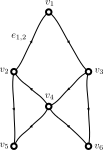
\includegraphics[scale=1.3]{directed_gm} \label{fig:dgm}
  }
  \hspace{1cm}
  \subfloat[]{%
  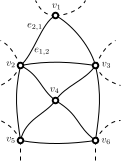
\includegraphics[scale=1.3]{undirected_gm} \label{fig:ugm}
  }
  }
  \caption[Examples of directed and undirected \acrshortpl{acr:gm}.]{Examples of directed and undirected \glspl{acr:gm}. \protect\subref*{fig:dgm}~Loop free directed \gls{acr:gm}. \protect\subref*{fig:ugm}~Loopy undirected \gls{acr:gm}.}
  \label{fig:gmExamples}
\end{figure}


Using a \gls{acr:gm} of a particular distribution, an inference algorithm can be devised based on the interactions between the latent variables in the model as well as the information propagating along its edges, therefore the following additional notations are required in order to simplify the formulation.
A random variable $U$ located on a vertex $v_i$ is denoted as $U_i$.
A message $m$ sent on an edge $e_{i,j}$ from vertex $i$ to vertex $j$ is denoted as $m_{ij}$.
It is worth noting that in undirected \glspl{acr:gm} where the edges $e_{i,j}$ and $e_{j,i}$ coexist, it is not necessarily true that the messages $m_{ij}$ and $m_{ji}$ are equal.

In essence, the messages in a \gls{acr:gm} describe a probability distribution in terms of either the target node variable $m_{ij}(U_j)$ or the source node variable $\eta_{ij}(U_i)$ which actually constitutes the flow of information in the \gls{acr:gm}.
Sometimes, we are interested in the joint distribution of a subset of random variables; if no confusion can arise, a subset of variables can simply be denoted as follows: if $c=\{1,2,\cdots,n\}$ then $U_c=\{U_1,U_2,\cdots,U_n\}$.
Similarly, a subset of vertices is denoted as $v_c=\{v_1,\cdots,v_n\}$.
The number of individual variables in $U_c$ is referred to as the cardinality of $U_c$ and is denoted by $\cardinal{U_c}$.


A clique $C(v_c)$ in a graph $\mathcal{G}(\mathcal{V},\mathcal{E})$ is a subset of nodes $v_c$ that are fully connected such that if $v_i,v_j \in v_c$, then $e_{i,j} \in \mathcal{E}$.
A clique is maximal if, and only if, there is no other node from outside the clique that can be added to it and still form a clique.
In other words, only a nonmaximal clique is a proper subset of a maximal clique.
The simplest example of a clique is a clique formed by any pair of nodes connected by an edge.
Also, any three nodes connected by three undirected edges form a clique. 


Undirected \glspl{acr:gm} represent a class of distributions that can be factorized based on cliques in the graph.
Let $\mathcal{C}$ be the set of maximal cliques in an undirected \gls{acr:gm},  then a family of distributions can be defined as follows:
\begin{equation}
	\mathcal{P}(U) = \frac{1}{Z} \prod_{C \in \mathcal{C}} \Psi_C(U_c) \label{eqn:maxcliqP}
\end{equation}
where $Z$ is a normalizing constant and $\Psi_c(U_c)$ is usually referred to as a compatibility function which also can be regarded as a local distribution of the clique variables $U_c$.
Such families of \glspl{acr:gm} are referred to as \gls{acr:mrf} or Gibbs distributions \cite{bib:Wainwright2008GMEFAVI}.
The maximal cliques requirement for \eqnRef{eqn:maxcliqP} can sometimes be relaxed to nonmaximal cliques.
For example, consider the following factorized distribution:
\begin{equation}
	\mathcal{P}(U) = \frac{1}{Z} \prod_{(i,j) \in E} \Psi_{i,j}(U_i,U_j) \prod_{i \in V} \Phi_i(U_i) \label{eqn:pwcliqP}
\end{equation}
where $\Psi_{i,j}(U_i,U_j)$ is referred to as the pairwise compatibility function and $\Phi_i(U_i)$ is the self potential function.
Distributions of this form can be represented by a \gls{acr:gm} that is pairwise connected, which we refer to as \gls{acr:pwgm}, where each vertex represents a variable node.


Since, in general, distributions corresponding to loopy undirected \glspl{acr:gm} contain factors that have coupled, or correlated, variable sets, inference on such models is not necessarily a trivial task.
However, the factorization structure of these distributions, as exposed by the \gls{acr:gm}, can be exploited by certain inference algorithms to produce computationally efficient algorithms. 


Distributions of the form \eqnRef{eqn:maxcliqP} are more conveniently represented using a special type of graph referred to as a \gls{acr:fg} \cite{bib:Kschischang2001FGATSA}.
\glspl{acr:fg} are bipartite graphs denoted as $\mathcal{G}(\mathcal{V},\mathcal{F},\mathcal{E})$, where there are two types of vertices, the vertex $v_i \in \mathcal{V}$ representing the variable nodes and the vertex $f_a \in \mathcal{F}$ representing the compatibility (or factor) functions $\Psi_a(U_a)$.
An edge $e_{i,a}$ in a \gls{acr:fg} connects a vertex $v_i \in \mathcal{V}$ to a vertex $f_a \in \mathcal{F}$ only when the corresponding vertex variable $U_i$ is an argument of the factor function $\Psi_a(U_a)$.
\figRef{fig:pw_vs_fg} shows a \gls{acr:pwgm} model and the corresponding \gls{acr:fg} with factor functions based on maximal cliques.
\glspl{acr:fg} are particularly useful when nonmaximal cliques are also configured; in such a case, different message update algorithms can be devised for the same problem resulting in different implementations with different numerical properties.
This feature will be exploited by our \gls{acr:fg} model for the \gls{acr:fem} problem, the \acrshort{acr:femfg} model, later introduced in \chpRef{chp:FGaBP}.
The \gls{acr:femfg} model can be used to produce variants of the \gls{acr:fgabp} algorithm, later described in \secRef{sec:elmMerg}, which has higher memory communication efficiency.  


\begin{figure}
	\centering
	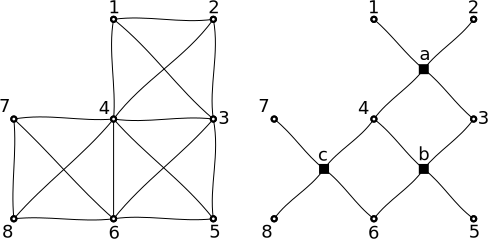
\includegraphics[scale=.9]{pw_vs_fg}
	\caption[The \acrshort{acr:pwgm} and the \acrshort{acr:fg} model.]{The \gls{acr:pwgm} (or \gls{acr:mrf}) on the left and the corresponding \gls{acr:fg} model configured with maximal cliques on the right, variable nodes are represented by circles and factor nodes are represented by squares.}
	\label{fig:pw_vs_fg}
\end{figure}


For general \glspl{acr:gm}, we will denote the number of variable nodes or vertices as \gls{acr:nv}, the number of edges as \gls{acr:ne} and the number of factor nodes, when present, as \gls{acr:nf}.
In addition, we will typically use small letters such as $n$ and $n_e$ to denote the local factor or clique quantities such as the number of vertices and edges correspondingly.



\section{The Belief Propagation Algorithm}
\label{sec:bp}


The \glsfirst{acr:bp} algorithm, as proposed by Pearl in \cite{bib:Pearl88ProbabilisticReasoning}, is a message passing algorithm on \gls{acr:gm} that efficiently computes the marginal distribution of each variable node by recursively sharing intermediate results.
If the \gls{acr:gm} is a tree, then \gls{acr:bp} is guaranteed to converge to exact marginals.
However, if the \gls{acr:gm} contains cycles, as typically the case in many practical applications, then \gls{acr:bp} takes an iterative form, referred to as \glsfirst{acr:lbp}, which can be used to obtain an approximation for the marginals \cite{bib:Pearl88ProbabilisticReasoning,bib:Yedidia2004CFEAAGBPA,bib:Weiss01CorrectnessBelief,bib:Wainwright03tbrfasp}.
\Gls{acr:bp} recently showed excellent empirical results in certain applications, such as machine learning, expert systems, computer vision, and channel decoding \cite{bib:Kschischang2001FGATSA, bib:Wainwright2008GMEFAVI,bib:Luby2001ILDPC,bib:Mceliece98turbodecoding,Richardson2001CLDPC,bib:cv1999,bibSun2003SMU,bib:Frey2001NIPS,bib:Kolmogorov2006ctr,bib:Weiss2005gobp,bib:Szeliski2008CS}.


\subsection{Belief Propagation on Factor Graph Models}


Executing \gls{acr:bp} on \glspl{acr:fg} consists of passing two types of messages.
A factor node message $m_{ai}$ sent from a factor node $\Psi_a$ to a connected variable node $U_i$; and a variable node message $\eta_{ia}$ sent back from the variable node $U_i$ to the factor node $\Psi_a$.
\Gls{acr:bp} messages on \gls{acr:fg} models are probability distributions; such that, the factor node message $m_{ai}$ constitutes a distribution in terms of the continuous random variable $U_i$, or the most probable state of $U_i$, as observed from the factor node $f_a$ with local function $\Psi_a$.
In return, the variable node message $\eta_{ia}$ constitutes a distribution in terms of $U_i$ by combining messages from all connected factor nodes excluding the message from the factor $f_a$.
The general \gls{acr:bp} update rules on \glspl{acr:fg} are formulated as follows:
\begin{align}
	m_{ai}^{(t)}(U_{i}) & \propto \underset{U_{\mathcal{N}(a)\setminus i}}{\int}\Psi_{a}(U_{a})\prod_{j\in\mathcal{N}(a)\setminus i}\eta_{ja}^{(t_\star)}(U_{j})\ \mathrm{d} U_{\mathcal{N}(a)\setminus i} \label{eqn:genFNUM}\\
	\eta_{ia}^{(t)}(U_{i}) & \propto \prod_{k\in\mathcal{N}(i)\setminus a}m_{ki}^{(t_\star)}(U_{i}) \label{eqn:genVNUM}\\
	b_{i}^{(t)}(U_{i}) & \propto \prod_{k\in\mathcal{N}(i)}m_{ki}^{(t)}(U_{i}) \label{eqn:genB}
\end{align}
where $t$ and $t_\star$ are iteration counts such that $t_\star \leq t$; \neih{a} is the set of all node indices connected to node $a$, referred to as the neighborhood set of node $a$; \neihMinus{a}{i} is the neighborhood set of $a$ minus node $i$ index; $b_i(U_i)$ is referred to as the belief at node $i$.  
The integral in \eqnRef{eqn:genFNUM} is a multidimensional integral of the random variable set $U_{\mathcal{N}(a)\setminus i}$ each integrated over all of their possible values.


It is important to note that message updates are performed according to a particular schedule.
For example, if we would use a fully parallel schedule, that is $t = t - 1$, then all factor and variable nodes will update their messages simultaneously based on the message values of the previous iteration; this update schedule is also referred to as synchronous update.
Alternatively we could traverse each variable or factor node sequentially based on a particular order, and then compute new messages based on the most recently available messages; this update schedule is also referred to as asynchronous updates.
Such a schedule does not offer the most potential for parallelism, but it was found empirically to exhibit the fastest to converge rate \cite{bib:Elidan06ResidualBP}.

\subsection{Belief Propagation on Pairwise Graphical Models}
\label{sec:pwgabp}


Considering \glspl{acr:pwgm} resulting from distributions with pairwise compatibility functions as shown in \eqnRef{eqn:pwcliqP}, each node sends and receives messages along all the pairwise edges connected to it.
Since variable nodes only communicate with other variable nodes of the same type, there can be only one type of message computed along the pairwise edges.
The general \gls{acr:bp} update rule for \glspl{acr:pwgm} is stated as follows:
\begin{equation}
	m_{ij}^{(t)}(U_j) \propto \underset{U_i}{\int}\Psi_{ij}(U_i,U_j)\Phi_i(U_i)\prod_{k\in\mathcal{N}(i)\setminus j}m_{ki}^{(t_\star)}(U_i)\mathrm{d} U_i. \label{eqn:genBPpw}
\end{equation}
The integral in \eqnRef{eqn:genBPpw} is taken for the single random variable $U_i$ over all its possible values.
A message $m_{ij}(U_j)$ is communicated from variable node $v_i$ to variable node $v_j$ over the edge $e_{i,j}$ using messages previously received from the neighborhood $\mathcal{N}(i)\setminus j$.
Once the messages converge, the marginal distribution for each variable can be obtained as:
\begin{equation}
	b_{i}^{(t)}(U_i) \propto \Phi_i(U_i) \prod_{k\in\mathcal{N}(i)}m_{ki}^{(t)}(U_i). \label{eqn:genBBPpw}
\end{equation}


\subsection{The Gaussian Belief Propagation Solver on Pairwise Graphical Models}


In this section we present a brief overview of the \glsfirst{acr:pwgabp} \cite{bib:Shental2008GBPSSLE,bib:Weiss01CorrectnessBelief} which was a recently introduced as a solver for linear systems of equations based on \gls{acr:bp} executed on \gls{acr:pwgm}.
While our initial experimentations with \gls{acr:pwgabp} for linear systems resulting from \gls{acr:fem} applications reveal that its performance does not match the existing state-of-the-art solvers such as \gls{acr:icpcg} and multigrid based solvers for large systems; it does offer however an important insight on the potential of using \gls{acr:bp} style algorithms to parallelize the \gls{acr:fem} problem as discussed in Chapters \ref{chp:PW-GaBP} and \ref{chp:relGaBP}.
In addition, the \gls{acr:pwgabp} requires the assembly of the large sparse linear system as in \eqnRef{eqn:aub} or the sparse matrix $A$, which is a costly step in the FEM process.


A Gaussian \gls{acr:pwgm} model is formulated by taking the exponential of the negated quadratic, defined in \eqnRef{eqn:quad}, as:
\begin{equation} 
	\label{eqn:maxGa}
	\mathcal{P}(U) = \frac{1}{Z}\exp(- \frac{1}{2}U^T A U + b^T U + c) 
\end{equation}
where $Z$ is a constant.
It can be shown that the solution of the linear system $u_{\star}=A^{-1}b$ is the maximum point of $\mathcal{P}$ which is also the point where the quadratic \eqnRef{eqn:quad} is minimum.
The exponential expression in (\ref{eqn:maxGa}) is a multivariate Gaussian probability distribution where the Gaussian mean vector $\mu$ equals the solution to the linear system $\mu = A^{-1} b$.
Hence the solution to the linear system can alternatively be obtained by executing the \gls{acr:bp} algorithm on the Gaussian \gls{acr:pwgm} represented by $\mathcal{P}$ in order to obtain its marginal means.

The Gaussian \gls{acr:pwgm} is constructed using the sparse matrix $A$ as follows.
The matrix $A$ can be viewed as an undirected graph where each nonzero element ($A_{ij} \neq 0$) represents an undirected edge between a pair of variable nodes indexed as $v_i$ and $v_j$.
Equivalently, we can factor the graph's distribution $\mathcal{P}$ into nodal functions $ \phi_i(U_i) \triangleq  \exp(- \frac{1}{2} A_{ii}U_i^2 + b_iU_i)$ and edge functions $\psi_{i,j}(U_i,U_j) \triangleq \exp(- \frac{1}{2} U_i A_{ij} U_j) $.
\gls{acr:bp} executing on Gaussian \gls{acr:pwgm} results in messages communicated between variable nodes as follows.
Each node $v_i$ computes a new message towards node $v_j$ on a particular edge $e_{i,j}$  using all messages received from nodes in the neighborhood $\mathcal{N}(i)$ of node $v_i$ excluding the message received from $v_j$.
The message update from each node is performed either sequentially or concurrently subject to a specific schedule.
Since the underlying distribution is Gaussian, the belief updates will be based on propagating only two parameters $\alpha$ and $\beta$, as shown below:
\begin{align}
\label{eqn_GaBPUpdateP}
\alpha_{ij}^{(t)} & = -A_{ij}^2 (\alpha_{i \setminus j}^{(t_\star)})^{-1} \\
\label{eqn_GaBPUpdateM}
\beta_{ij}^{(t)} & = -A_{ij} \beta_{i \setminus j}^{(t_\star)} (\alpha_{i \setminus j}^{(t_\star)})^{-1} \\
\intertext{where:}
\label{eqn_a_i_minus_j_bc}
\alpha_{i \setminus j}^{(t_\star)} & =  \alpha_i^{(t_\star)} - \alpha_{ji}^{(t_\star)} \\
\label{eqn_b_i_minus_j_bc}
\beta_{i \setminus j}^{(t_\star)} & = \beta_i^{(t_\star)} - \beta_{ji}^{(t_\star)} \\
\intertext{and:}
\alpha_i^{(t)} & = A_{ii} + \sum_{k \in N(i)} \alpha_{ki}^{(t)} \\
\beta_i^{(t)} & = b_i + \sum_{k \in N(i)} \beta_{ki}^{(t)} .
\end{align}


For large sparse systems, the overall \gls{acr:pwgabp} computational complexity per iteration is $\bigo{lN}$,  where $N$ is the number of unknowns and $l$ is a constant ($l \ll N$) determined by the sparsity of the underlying problem, for example the average number of links per node.  
The marginal means, constituting the approximate solution, can then be computed by:
\begin{equation}
\label{eqn_x_i}
\bar{U}_i^{(t)} = \frac{\beta_i^{(t)}}{\alpha_i^{(t)}}. 
\end{equation}





GaBP was shown in \cite{bib:Johnson2006WIAGBP} to converge for a particular class of matrices referred to as the walk-summable model.
The walk-summability condition states that the spectral radius of the normalized off-diagonals of $A$ is less than 1 in the absolute sense, that is $\rho(\vert I - D^{-\frac{1}{2}} A D^{-\frac{1}{2}}\vert) < 1$, where $D$ is the diagonal elements of $A$.
Such class of matrices includes the symmetric positive-definite diagonally dominant systems that arise from many \gls{acr:fem} applications.
\gls{acr:pwgabp} is one of the algorithms implemented by the parallel library Graphlab \cite{bib:graphlab2010} aimed primarily at machine learning applications.


\section{Convergence Testing}
\label{sec:convtest}
In practical implementations of the Gaussian \gls{acr:bp} algorithms, the $l^2$-norm of the differences in the successive approximate solutions, the relative norm for short, can be used as a computationally efficient measure to test the convergence of the algorithm.
The relative norm ($e_r$) is computed as follows:
\begin{align} 
	e^{(t)}_r & =  \frac{\parallel \bar{u}^{(t)} - \bar{u}^{(t-1)} \parallel_2}{\parallel \bar{u}^{(t)} \parallel_2} \notag \\
		& = \left(\frac{\sum_{i=1}^{N} (\bar{u}_i^{(t)} - \bar{u}_i^{(t-1)})^2} {\sum_{i=1}^{N} (\bar{u}_i^{(t)})^2}\right)^{\frac{1}{2}} \label{eq_relErr}
\end{align}
where $(t)$ is the iteration number, $\bar{u}^{(t)}$ is the solution vector estimate at iteration $(t)$ and $\bar{u}_i$ is the solution estimate at node $i$.
The algorithm can be terminated when the relative norm reaches a certain tolerance value.
The relative norm is also used for our development of the faster convergent relaxed \gls{acr:pwgabp} algorithm introduced in \chpRef{chp:relGaBP}.

Another measure for convergence is the normalized residual $l^2$-norm, which is computed as follows:
\begin{equation} 
	R^{(t)} = \frac{\parallel b - A\bar{u}^{(t)} \parallel_2}{\parallel b \parallel_2}
\end{equation}
The residual $R$ provides an upper bound for the relative norm; however, the relative norm is used in practice for \gls{acr:pwgabp} to test convergence since it is less costly to compute by avoiding the \gls{acr:smvm} operation ($A\bar{u}^{(t)}$).
However, in \gls{acr:cg} and multigrid algorithms, the residual is typically used for convergence testing since it is iteratively computed as part of these algorithms.
In addition, the residual is used as the final convergence verification criteria in our experiments when we compare different algorithms.

\section{The Condition Number and Diagonal Dominance} 
\label{sec:cndd}
The Condition number of a matrix is defined as:
\begin{equation}
k\left(A\right) \triangleq \frac{\lambda_{max}\left(A\right)}{\lambda_{min}\left(A\right)}
\end{equation} 
where $\lambda_{max}\left(A\right)$ and $\lambda_{min}\left(A\right)$ are the largest and smallest eigenvalues of $A$.
In numerical linear algebra, the condition number measures the sensitivity of the solution of the linear system to small perturbations in $A$.
It may also be used to bound the convergence rate of iterative solvers of linear systems.
Well-conditioned matrices have $k\left(A\right)\approx 1$ while ill-conditioned matrices can have a much larger condition number.

The matrix $A$ is known to be \gls{acr:wdd} if 
\begin{equation}
|a_{ii}| \geq \sum_{j\neq i} |a_{ij}| \quad\text{for all } i, \label{eq:diagDom}
\end{equation}
with strict inequality ($>$) for at least one index $i$.
If the inequality is replaced by ($>$) for all $i$, then the matrix $A$ is referred to as \gls{acr:sdd}.


\section{Speedup}


The execution time speedup (\gls{acr:su}) is the performance measure used in our experiments.
The \gls{acr:su} is defined as the ratio of the execution times of two algorithms or implementations and computed as follows:
\begin{equation}
	\text{SU} = \frac{\text{execution time of algorithm $Y$}}{\text{execution time of algorithm $X$}}
	\label{eqn:suET}
\end{equation}
which states the speedup of algorithm $X$ over algorithm $Y$.
If algorithm $X$ is the parallel implementation of a sequential algorithm $Y$, then this is referred as the parallel \gls{acr:su}.

%==========
\graphicspath{{./figs/Chp-PWGaBP/}}

%%Fakesection Acronym reset
\glsreset{acr:pwgabp}
\glsreset{acr:sdd}
\glsreset{acr:dpcg}
\glsreset{acr:sus}
\glsreset{acr:pus}
\glsreset{acr:hus}
\glsreset{acr:pwgm}
\glsreset{acr:rcm}

\chapter{Schedule Implementations for Gaussian Belief Propagation}


\label{chp:PW-GaBP}
In this chapter, we introduce implementation-oriented scheduling schemes for the \gls{acr:pwgabp} solver aimed at large sparse linear systems obtained from \gls{acr:fem} applications.
We analyze different message scheduling schemes used to enhance implementations, CPU time, and parallel executions.
Our empirical experiments show that \gls{acr:pwgabp} when used with \gls{acr:sdd} matrices can potentially result in execution-times that are competitive with the widely used \gls{acr:dpcg} solver.


We present empirical results of the \gls{acr:sus} of the \gls{acr:pwgabp} solver.
Compared with the \gls{acr:dpcg} solver, the \gls{acr:sus} demonstrates considerable reduction in iteration count for large sparse \gls{acr:sdd} linear systems.
Next, we present the \gls{acr:hus} for the \gls{acr:pwgabp}.
The \gls{acr:hus} algorithm uses an appropriate mix of sequential and parallel message updates.
The parallel implementations of the \gls{acr:hus} demonstrates that, the \gls{acr:hus} facilitates efficient parallel execution while demonstrating faster convergence rates typical of \gls{acr:pwgabp} using \gls{acr:sus}.


\section{Introduction}

In this work, we present various scheduling implementations for the \gls{acr:pwgabp} to solve large sparse linear systems arising from the \gls{acr:fem} problem.
We, therefore, assume that the sparse matrix $A$ for the underlying \gls{acr:fem} problem is already assembled by other \gls{acr:fem} software such as \libName{GetFEM} \cite{bib:getfem}.
The computational efficiency of a \gls{acr:pwgabp} implementation will depend largely on two factors: the data-structure used to store the nodes' connectivities as provided by the \gls{acr:pwgm} along with communicated messages, and the message transfer medium such as the memory bandwidth for shared-memory architectures or the network bandwidth for CPU-clusters.
From an implementation perspective, three distinct stages can be designated for the nodal message update process of the \gls{acr:pwgabp} algorithm.
First, the node receives messages from sparse connections.
Second, the node performs local computations using the received messages.
Last, the node responds with new messages on the same sparse connections.
For CPU implementations, the choice of the data-structure required to store the messages will have a critical impact on the overall performance of the \gls{acr:pwgabp} algorithm due to the predominant message access time, data-locality and vectorization of computational loops.
However, sparse matrices arising from typical \gls{acr:fem} applications can exhibit a banded sparsity structure when proper reordering algorithms are used, which can be exploited to increase the parallel \gls{acr:pwgabp} performance.


\gls{acr:pwgabp} message updates are performed subject to a particular schedule.
Two basic scheduling schemes common in general \gls{acr:bp} algorithms are the \gls{acr:sus}, and the \gls{acr:pus}, also known as flooding.  
In the \gls{acr:sus}, nodes are processed in sequence according to a particular ordering; while messages are propagated sequentially to receiving nodes in the same iteration.  
Hence, the \gls{acr:sus} scheme provides little opportunity for parallel processing.
The \gls{acr:pus}, on the other hand, facilitates fully concurrent execution of the nodes; however, the \gls{acr:pus} requires a considerably larger number of iterations compared to \gls{acr:sus}.
Specifically, the empirical analysis in \cite{bib:Elidan06ResidualBP,bib:Bertsekas1983DACFP} and other references within, indicates that the convergence rate of the \gls{acr:sus} is upper-bounded by the convergence rate of the \gls{acr:pus}.
The work in \cite{bib:Elidan06ResidualBP,bib:gonzalez2009residual} also uses an informative based scheduling scheme which is used to accelerate convergence; in addition this scheme, in certain cases, can achieve convergence for models where basic \gls{acr:bp} fails.  
However, this work mainly uses discrete-domain probabilistic models of relatively small size compared to the large models resulting from \gls{acr:fem} applications where the number of real-domain variables range in the order of millions or billions.
Therefore, we believe that the \gls{acr:bp} scheduling for \gls{acr:fem} problems should be treated as an implementation feature to enhance parallelism of the algorithm rather than to improve the convergence rate.
The convergence rate, on the other hand, can more efficiently be treated using a specialized multigrid scheme for \gls{acr:bp} as we later show in \chpRef{chp:FMGaBP}.


This chapter is organized as follows.
In \secRef{sec:sus} we present the \gls{acr:sus} implementation of the \gls{acr:pwgabp} algorithm. 
In \secRef{sec:pus} we present the \gls{acr:pus} implementation.
In \secRef{sec:hus} we present the \gls{acr:hus} implementation.
Finally, in \secRef{sec:pwgabpRes} we conclude with performance results.

\section{Sequential Update PW-GaBP}
\label{sec:sus}


In \algRef{alg:seq_gabp} we present a particular implementation of \gls{acr:pwgabp} which makes efficient use of contiguous data-structures such as queues or stacks to store and retrieve messages.
This particular implementation uses the \gls{acr:sus} scheme.
Using simple data-structures such as stacks or queues results in constant-time per message access complexity for retrieval and insertion, reducing the algorithm's overall message processing complexity per iteration to $\bigo{\gls{acr:nnz}}$, where \gls{acr:nnz} is the number of non-zeros in $A$.
Using such data-structures is facilitated by adding the source node pointer ($n_i$) and the edge element parameter ($A_{i,j}$) to the message.
Stacks are used in all our implementations; however, queues can also be used instead of stacks without much impact on the algorithm's performance.  
It is important to note that this implementation results in a fixed increase in the memory requirement per each message.  
However, since this fixed increase in the message size is independent of the problem's overall size $N$, where $N$ is the number of variables, the algorithm's overall memory complexity scales linearly with $N$ as expected for sparse problems.


In the \gls{acr:sus}, the nodes need to be processed according to a particular order.
In addition, the initialization stage is critical for the correct operation of the algorithm.
As shown in lines 2 to 6, a unique nodal ordering ($\kappa$) needs to be defined.
The nodes are also initialized with zero messages subject to the ordering $\kappa$.
In this algorithm, a single processing node is assumed that has access to the full data-structure of $A$.
While the \gls{acr:sus} is not practical for parallel implementations, its study provides a hypothetical lower bound on the iteration count of the \gls{acr:pwgabp} solver when used with linear systems resulting from \gls{acr:fem} applications.

% Sequential version of \gls{acr:pwgabp} Algorithm
\begin{algorithm}[h]
	\centering
	\begin{algorithmic}[1]

		\STATE \textit{Initialize: }

		\STATE Define node ordering: $ \kappa $

		\FOR{each edge $A(i,j)$}

		\IF{$ n_i <_{\kappa} n_j$}
		\STATE $n_i.\OpN{push}(n_j.\OpN{pointer},A_{ij}, P_{ji} = 0, \mu_{ji} = 0) $
	\ENDIF

\ENDFOR

\STATE \textit{Compute: }
\REPEAT[iterations]
\FOR{ each node $n_i \in \kappa $}
\STATE $ P_{agg} = A_{ii} + \sum_{k} P_{ki}$
\STATE $ \mu_{agg} = b_{i} + \sum_{k} \mu_{ki}$

\FOR{ each received message $n_j \rightarrow n_i$ }
\STATE $\mu_{ij} = -A_{ij} (P_{agg} - P_{ji})^{-1} (\mu_{agg} - \mu_{ji}) $
\STATE $P_{ij} = -A_{ij}^2 (P_{agg} - P_{ji})^{-1} $
\STATE $n_i.\text{pop\_message}$
\STATE $n_j.\OpN{push}(n_i.\OpN{pointer},A_{ij}, P_{ij}, \mu_{ij})$
\ENDFOR
\STATE $\overline{x_i} = \mu_{agg} P_{agg}^{-1}$

\ENDFOR
\UNTIL{\textit{convergence:} all $\overline{x_i}$ converged}
\STATE \textit{Output:} $\overline{x_{i}}$
\end{algorithmic}

\caption{The sequential update \acrshort{acr:pwgabp} implementation-oriented algorithm.}
\label{alg:seq_gabp}
\end{algorithm}

\section{Parallel Update PW-GaBP}
\label{sec:pus}

The \gls{acr:pus} version of the \gls{acr:pwgabp} algorithm is shown in \algRef{alg:par_gabp}.
This algorithm uses arrays of local static memory to store the node's edge messages.
The local memory array provides constant time access on shared-memory machines by assigning a specific memory location to each destination node.
To facilitate concurrent execution of all nodes, each node contains two message arrays, a current-message array that stores messages received in the previous iteration and is used to compute the new messages in the current iteration, and a new-message array that is used to store the new messages being received from the edge nodes in the current iteration.
Alternately, coloring schemes can be used to resolve memory collisions as proposed later in \chpRef{chp:FMGaBP}.
At the beginning of each iteration, each node collects its edge messages into the new message buffer then swaps the current and the new message buffer pointers.
Constant-time access data-structures such as queues and stacks can be used instead of static memory arrays.
Also, there is no need to define any node ordering as the case in the \gls{acr:sus} algorithm.
Since the number of processing elements in computing environments is typically much less than the number of nodes, the \gls{acr:pus} algorithm may not be practical for implementations targeted for large linear systems; nonetheless, the algorithm has conceptual importance for approximating the upper bound on the parallel iteration count.

% Parallel version of \gls{acr:pwgabp} Algorithm
\begin{algorithm}[h]
	\centering
	\begin{algorithmic}[1]
		\STATE \textit{Initialize:}
		\FOR{each edge $A(i,j)$}
		\STATE $n_i.\OpN{send}(n_j.\OpN{pointer},A_{ij}, P_{ji} = 0, \mu_{ji} = 0)$
		\AlgENDFOR
		\STATE \textit{Compute: }
		\REPEAT[iterations]
		\FOR{each node $n_i$ }
		\STATE $n_i.\OpN{swap\_pointers}(\OpN{currMessArray},\OpN{newMessArray})$
		\AlgENDFOR
		\FOR[concurrent execution]{ each node $n_i$ }
		\STATE Using the current-message buffers
		\STATE $ P_{agg} = A_{ii} + \sum_k P_{ki}$
		\STATE $ \mu_{agg} = b_{i} + \sum_k \mu_{ki}$
		\FOR{each received message $n_j \rightarrow n_i$ }
		\STATE $\mu_{ij} = -A_{ij} (P_{agg} - P_{ji})^{-1} (\mu_{agg} - \mu_{ji}) $
		\STATE $P_{ij} = -A_{ij}^2 (P_{agg} - P_{ji})^{-1} $
		%\STATE $n_i.\OpN{pop\_message}$
		\STATE $n_j.\OpN{send}(n_i.\OpN{pointer},A_{ij}, P_{ij}, \mu_{ij})$
		\AlgENDFOR
		\STATE $\overline{x_i} = \mu_{agg} P_{agg}^{-1}$
		\AlgENDFOR
		\UNTIL{\textit{convergence:} all $\overline{x_i}$ converged}
		\STATE \textit{Output:} $\overline{x_{i}}$
	\end{algorithmic}
	\caption{The parallel update \acrshort{acr:pwgabp} implementation-oriented algorithm.}
	\label{alg:par_gabp}
\end{algorithm}


\section{Hybrid Update PW-GaBP}
\label{sec:hus}

Since in typical parallel computing environments the number of processing elements is limited, a degree of sequential processing will have to be performed for large problems.
Our implementation-oriented \gls{acr:hus} algorithm, shown in \algRef{alg:hyb_gabp}, takes advantage of this imposed sequentiality to propagate faster message information, which reduces the \gls{acr:pwgabp} iteration count while exploiting parallelism in both single-node and multi-node \glspl{acr:hpc}.


By creating a partitioning scheme of relatively adjacent nodes, where each partition is assigned to a processing element to be executed in parallel, updates between nodes in different partitions can be performed using the \gls{acr:pus} algorithm, while updates between nodes in the same partition can be performed using the \gls{acr:sus} algorithm.
This flexibility allows the \gls{acr:hus} algorithm to easily implement different sequential-parallel scheduling variations by varying the partition boundaries and the node ordering within each partition.
That is, by choosing a partitioning and an ordering scheme that exploits node locality in terms of connectivity.
The number of iterations increase due to parallel message updates can be expected to be considerably reduced, which will be demonstrated later in our results.

% Hybrid version of \gls{acr:pwgabp} Algorithm
\begin{algorithm}[!t]
	\centering
	\begin{algorithmic}[1]
		\small
		\STATE \textit{Initialize:}
		\STATE Define node partitioning $\zeta $
		\STATE Define node ordering $\kappa$ in each $\zeta$
		\FOR{each edge $A(i,j)$}
		\IF[nodes in the same partition]{$n_i =_\zeta n_j$}
		\IF{$ n_i <_{\kappa} n_j$}
		\STATE $n_i.\OpN{push}(n_j.\OpN{pointer},A_{ij}, P_{ji} = 0, \mu_{ji} = 0) $
		\AlgENDIF
		\ELSE[nodes not in the same partition]
		\STATE $n_i.\OpN{send}(n_j.\OpN{pointer},A_{ij}, P_{ji} = 0, \mu_{ji} = 0)  $
		\AlgENDIF
		\AlgENDFOR
		\STATE \textit{Compute: }
		\REPEAT[iterations]
		\FOR{ each node $n_i$ on partition edge }
		\STATE $n_i.\OpN{swap\_pointers}(\OpN{currMessArray},\OpN{newMessArray})$
		\AlgENDFOR
		\FOR[concurrent execution] { each partition in $\zeta $}
		\FOR[sequential execution]{ each node $n_i \in \kappa$ }
		\STATE $ P_{agg} = A_{ii} + \sum_k P_{ki}$
		\STATE $ \mu_{agg} = b_{i} + \sum_k \mu_{ki}$

		\FOR{ each received message $n_j \rightarrow n_i$ }
		\STATE $\mu_{ij} = -A_{ij} (P_{agg} - P_{ji})^{-1} (\mu_{agg} - \mu_{ji}) $
		\STATE $P_{ij} = -A_{ij}^2 (P_{agg} - P_{ji})^{-1} $
		\IF{$n_j$ in the same partition}
		\STATE $n_i.\OpN{pop\_message}$
		\STATE $n_j.\OpN{push}(n_i.\OpN{pointer},A_{ij}, P_{ij}, \mu_{ij})$
		\ELSE
		\STATE $n_j.\OpN{send}(n_i.\OpN{pointer},A_{ij}, P_{ij}, \mu_{ij})$
		\AlgENDIF
		\AlgENDFOR
		\STATE $\overline{x_i} = \mu_{agg} P_{agg}^{-1}$
		\AlgENDFOR

		\AlgENDFOR
		\UNTIL{\textit{convergence:} all $\overline{x_i}$ converged}
		\STATE \textit{Output:} $\overline{x_{i}}$
	\end{algorithmic}
	\caption{The hybrid update \gls{acr:pwgabp} implementation-oriented algorithm.}
	\label{alg:hyb_gabp}
\end{algorithm}


\section{Results and Discussions}
\label{sec:pwgabpRes}



\subsection{Performance Comparison with D-PCG}


In order to assess the computational speed of the \gls{acr:sus}, we compare it with the \gls{acr:dpcg} algorithm.
All runs are executed on single CPU workstation with Intel Core2 Quad @ 2.8GHz using double-precision computations.
The \gls{acr:dpcg} code was executed on the same CPU and it was obtained from the optimized \libName{GMM++} library \cite{bib:gmm}.
Iterations were stopped when the $l^2$-norm of the residual reached $\epsilon = 10^{-9}$.
The test matrices, shown in \tableRef{tbl:testMatrices}, are obtained from \cite{bib:UFSparseMatrix}, with the exception of the matrix ``Random'' which is generated randomly using the Matlab software \cite{bib:matlab2013}.
The matrix ``thermal2'' results from an unstructured steady-state \gls{acr:fem} application.
The matrices were made diagonally dominant by loading the diagonals with a uniformly distributed positive random number having a standard deviation $\sigma \in [10^{-2},10^3]$, in order to make the matrices conform with the walk-summability criteria \cite{bib:Johnson2006WIAGBP} required for the \gls{acr:pwgabp} convergence.
The plots in \figRef{fig:su} show the performance results of the \gls{acr:pwgabp} solver using the \gls{acr:sus} scheme against the \gls{acr:dpcg} solver.
Iteration reductions, up to 6$\times$, are obtained by the \gls{acr:sus} \gls{acr:pwgabp} algorithm.
Also, the \gls{acr:sus} implementation was able to achieve time speedups for many cases reaching up to 1.8$\times$.
It is worth noting that the obtained time speedup gains do not match the gains from the iteration reductions, which we attribute to the fact that the \libName{GMM++} implementation of the \gls{acr:dpcg} algorithm has more efficient memory bandwidth utilization for sequential execution than our algorithm.
However, the \gls{acr:pwgabp} algorithm is more tailored towards parallel implementations than the \gls{acr:pcg} algorithm.

\begin{table}
	\centering
	\begin{threeparttable}[c]
		\caption{Sparse test matrices.}
		\label{tbl:testMatrices}
		\centering
		%\begin{tabular}{lcccc}
		\begin{tabular}{ >{\centering\arraybackslash}m{.7in}  >{\centering\arraybackslash}m{.7in}  >{\centering\arraybackslash}m{.9in}  >{\centering\arraybackslash}m{.7in}  >{\centering\arraybackslash}m{.7in} }
			\toprule
			\flushleft Category & ecology1 & G3{\_}circuit & thermal2 & random\\
			\midrule
			\flushleft N (nodes) & 1,000,000 & 1,585,478 & 1,228,045 & 1,000,000 \\
			\flushleft $\OpN{nnz} $ & 4,996,000 & 7,660,826 & 8,580,313 & 8,999,976 \\
			\bottomrule
		\end{tabular}
	\end{threeparttable}
\end{table}

%%
\begin{figure}[!t]
	\centerline{
	\subfloat[]{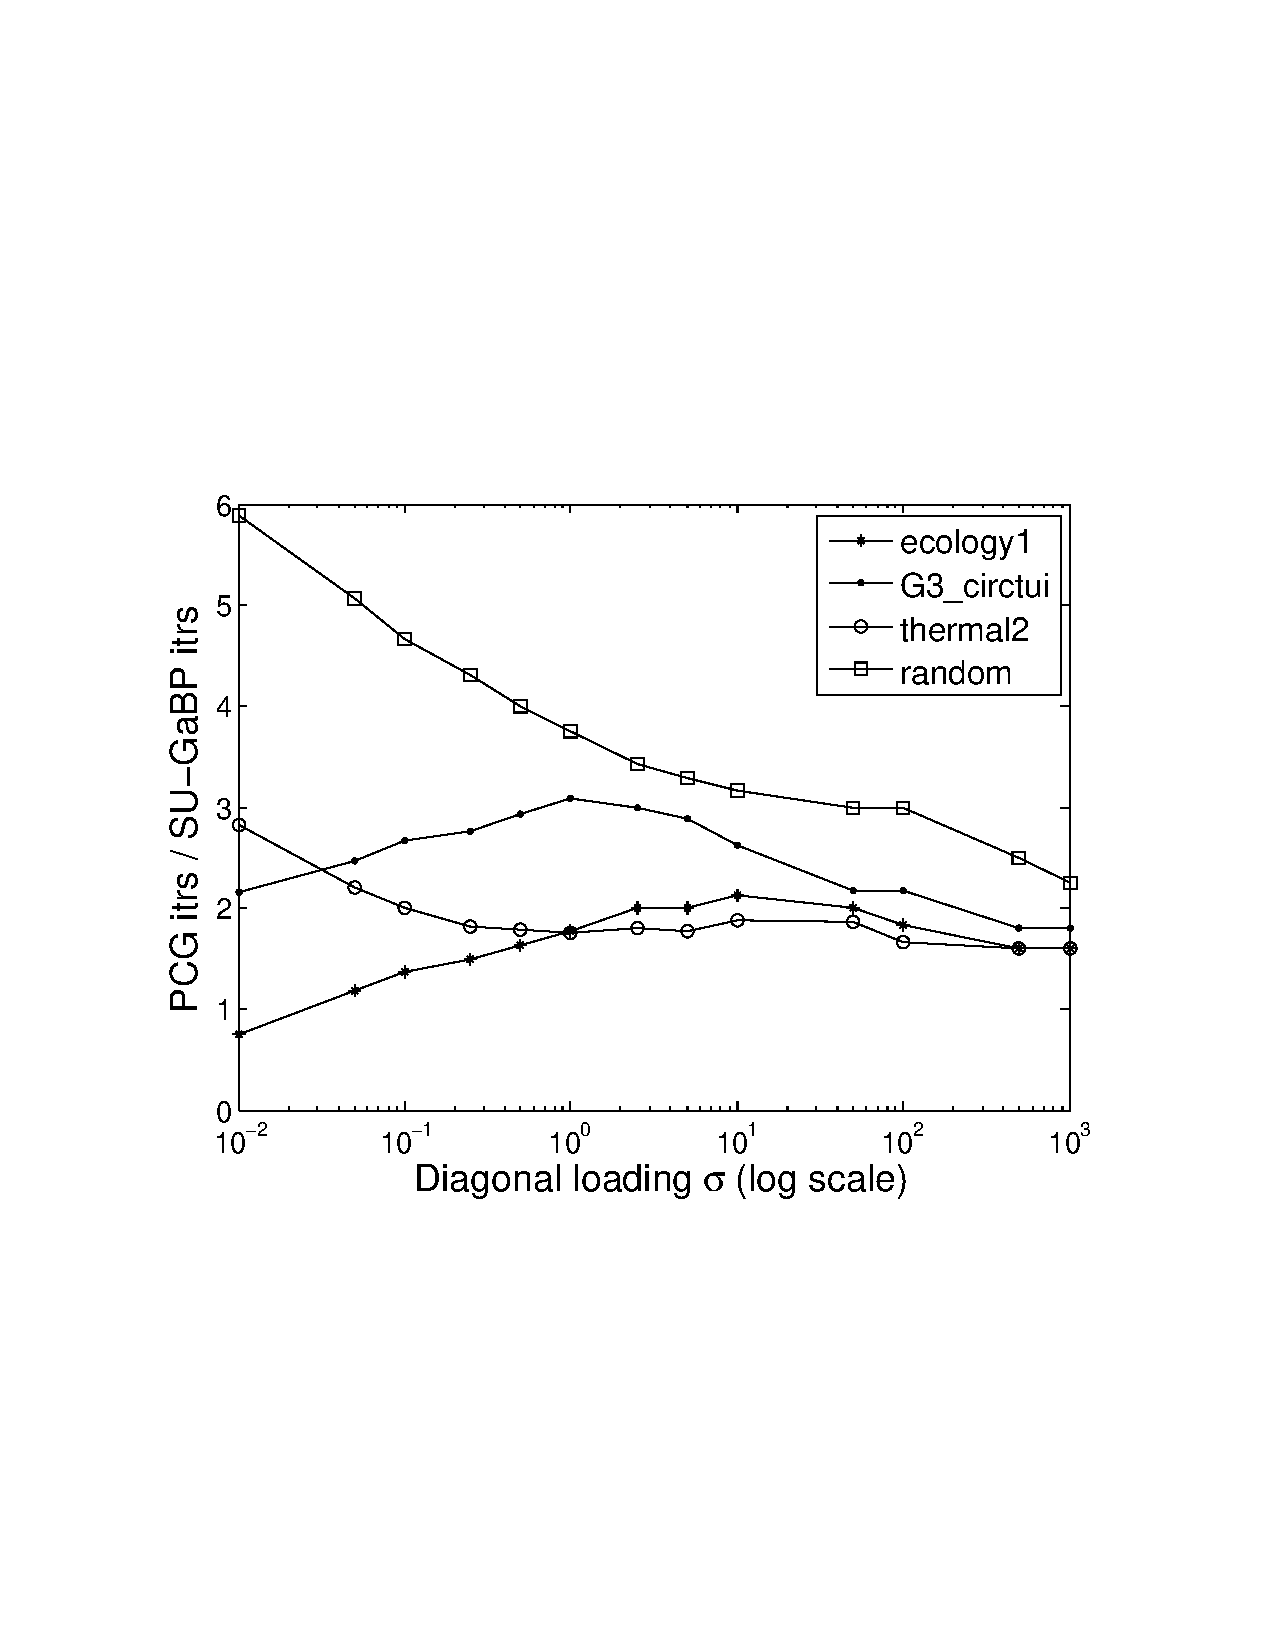
\includegraphics[width=2.8in]{FIG2}}
	\hfill
	\subfloat[]{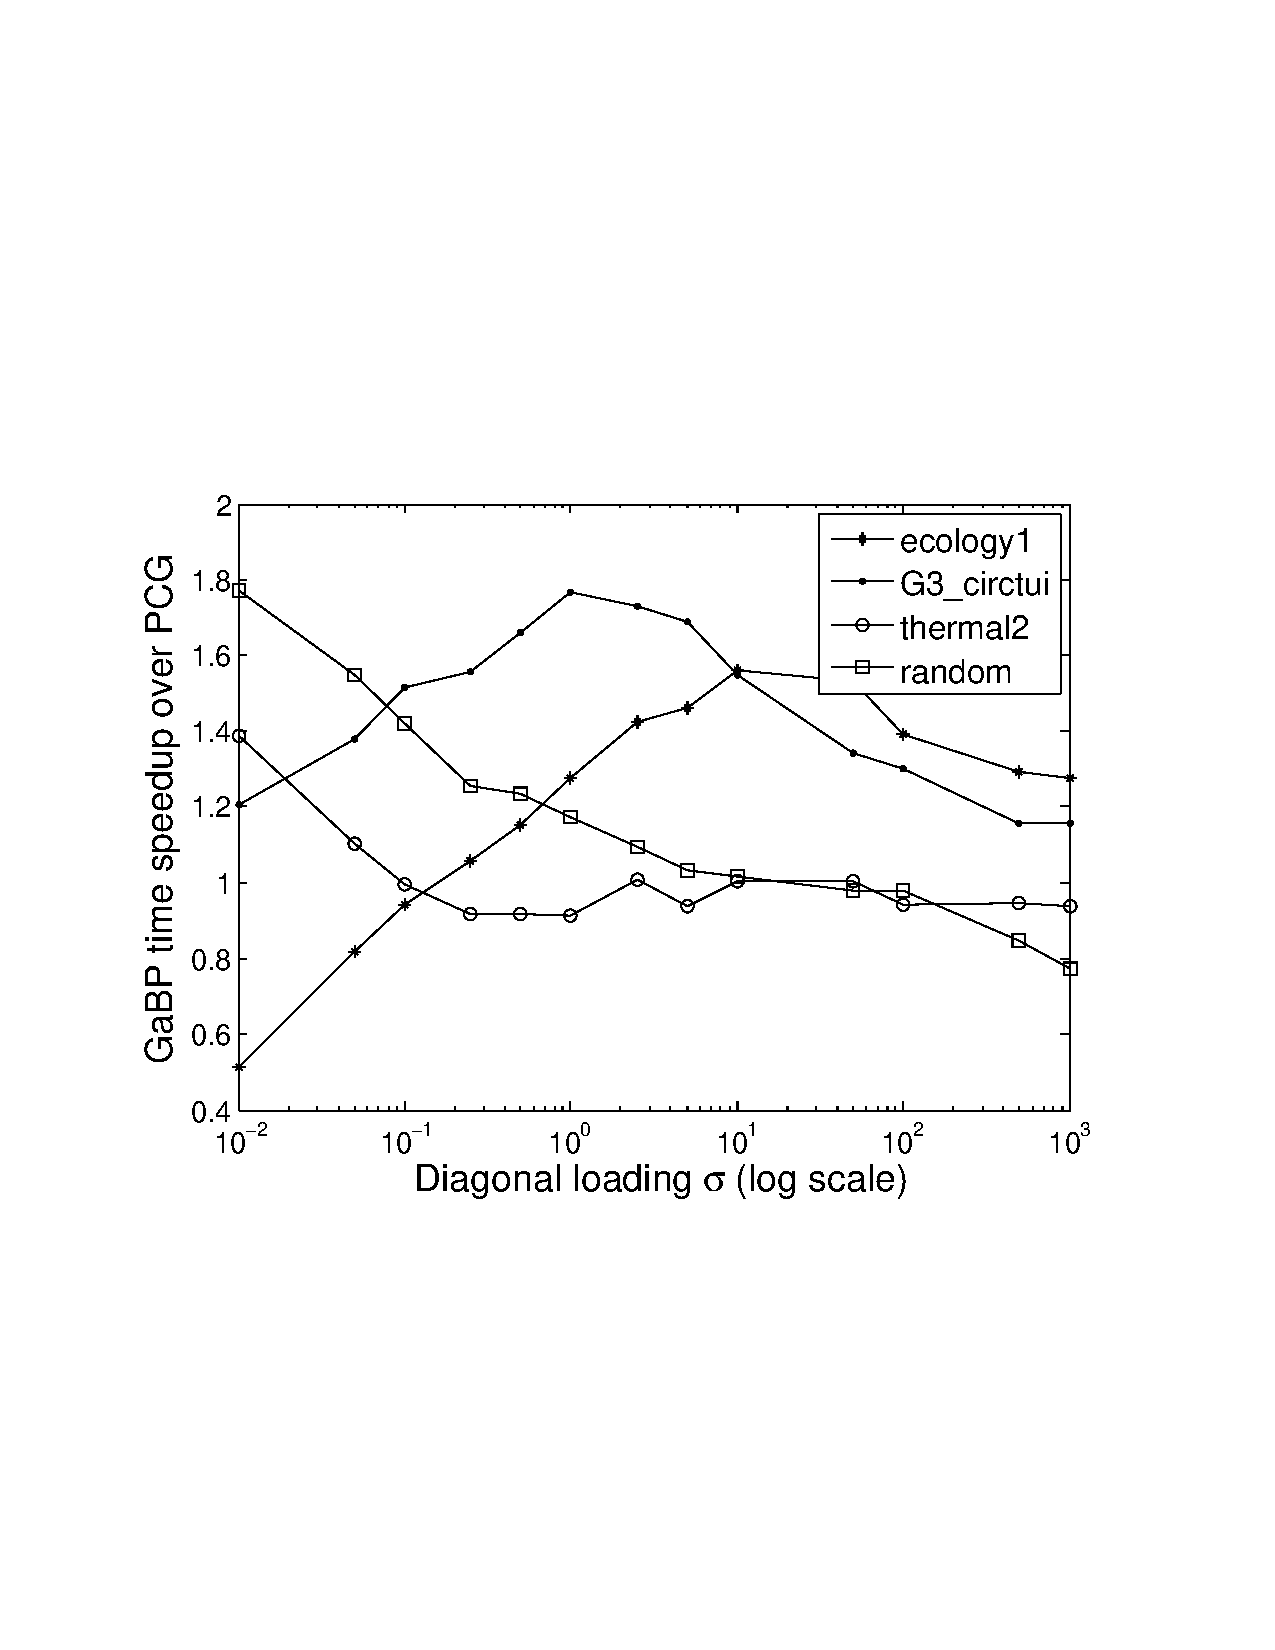
\includegraphics[width=2.8in]{FIG3}}
	}
	\caption[Speedup of the \acrshort{acr:pwgabp} implementation over \acrshort{acr:dpcg}.]{Speedup of the implementation-oriented \gls{acr:pwgabp} using the \gls{acr:sus} scheme. (a) Iteration improvement of \gls{acr:pwgabp} over \gls{acr:dpcg}. (b) \gls{acr:pwgabp} time speedup over \gls{acr:dpcg}.}
	\label{fig:su}
\end{figure}

\subsection{Hybrid-Update Scheduling Performance}

The parallel behavior of the \gls{acr:pwgabp} algorithm using the \gls{acr:hus} implementation was simulated on a single-core CPU.
In order to simulate different partitioning and node ordering, matrix reordering techniques were used.
Two common reordering techniques used here are: the \gls{acr:rcm} \cite{bib:Cuthill1969RTBOSSM}, which reduces the matrix bandwidth; and \gls{acr:amd}, which produces large blocks of zeros \cite{bib:George1989TEOTMDOA}. 
\figRef{fig:hu-gabp} shows the parallel results of our \gls{acr:hus} implementation algorithm on the matrix ``thermal2'' as the number of parallel partitions increases from 1 to 4096.
The \gls{acr:hus} algorithm demonstrates gradual rate of increase in iterations on the original unordered matrix, while ordered matrices using the \gls{acr:rcm} and the \gls{acr:amd} algorithms showed a considerably lower rate of increase.
These results demonstrate the \gls{acr:hus} potential for parallel gains and its ability in exploiting the problem's connectivity structure by maintaining a lower iteration count than the \gls{acr:pus} scheme.
These results also suggest that good speedup gains can be obtained from implementing the \gls{acr:hus} on CPU-clusters and many-core architectures in comparison with leading iterative methods such as the \gls{acr:dpcg} algorithm.

\begin{figure}
	\centerline{
	\subfloat[]{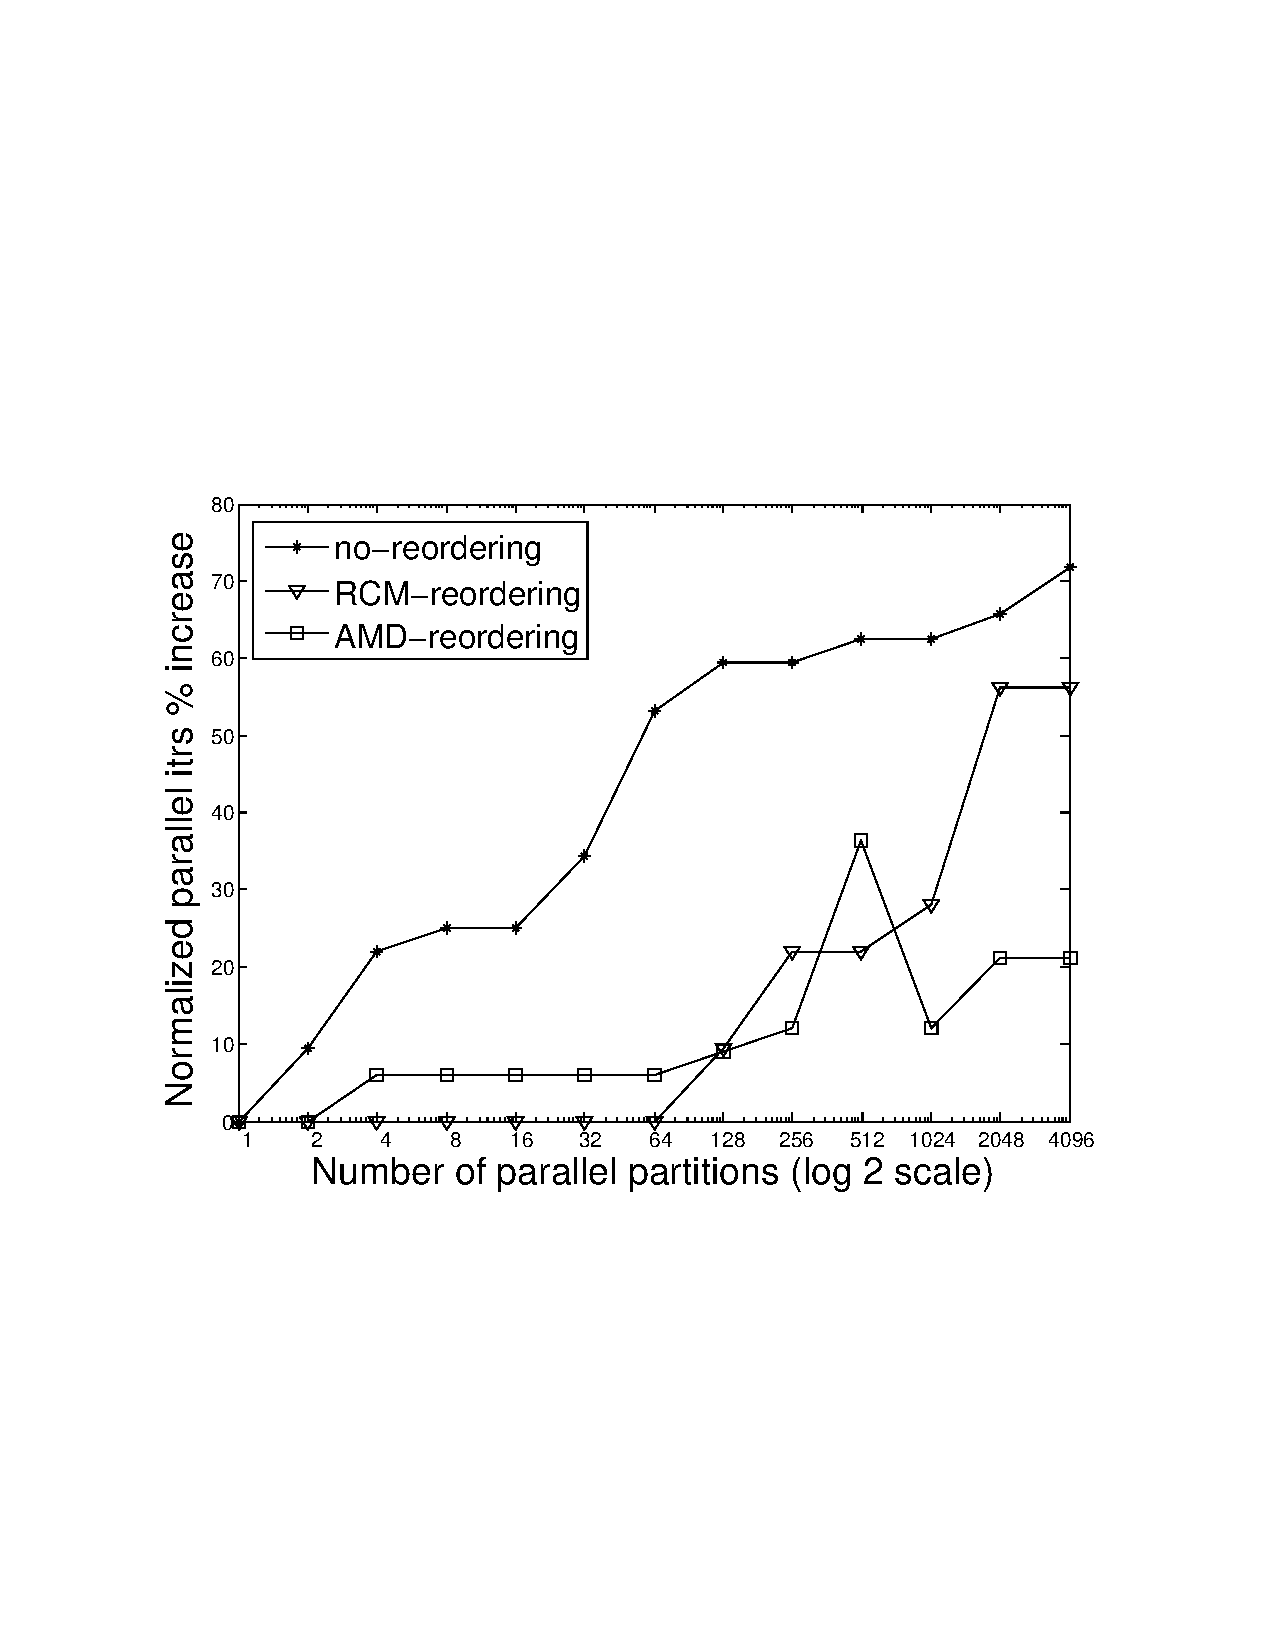
\includegraphics[width=3.0in]{FIG4}}
	}
	\centerline{
	\subfloat[]{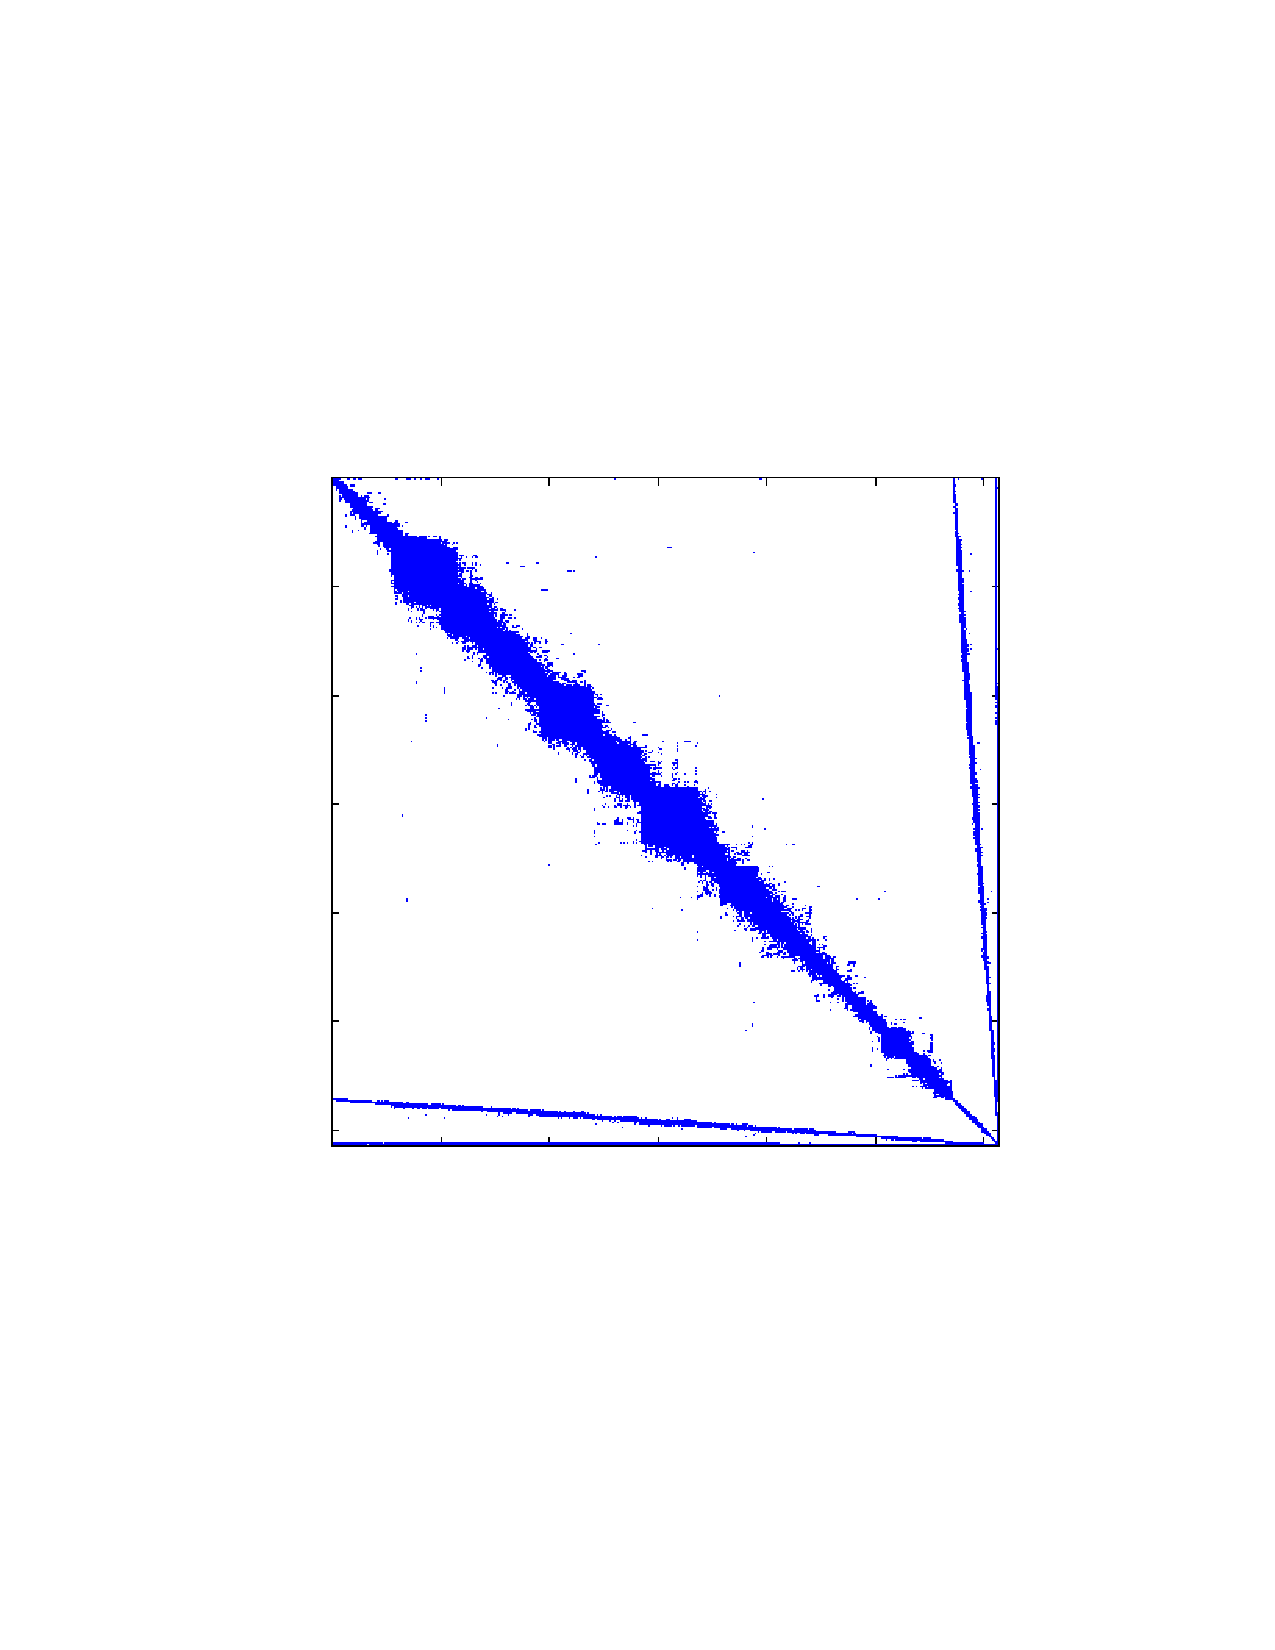
\includegraphics[width=.8in]{FIG5}}
	\hfil
	\subfloat[]{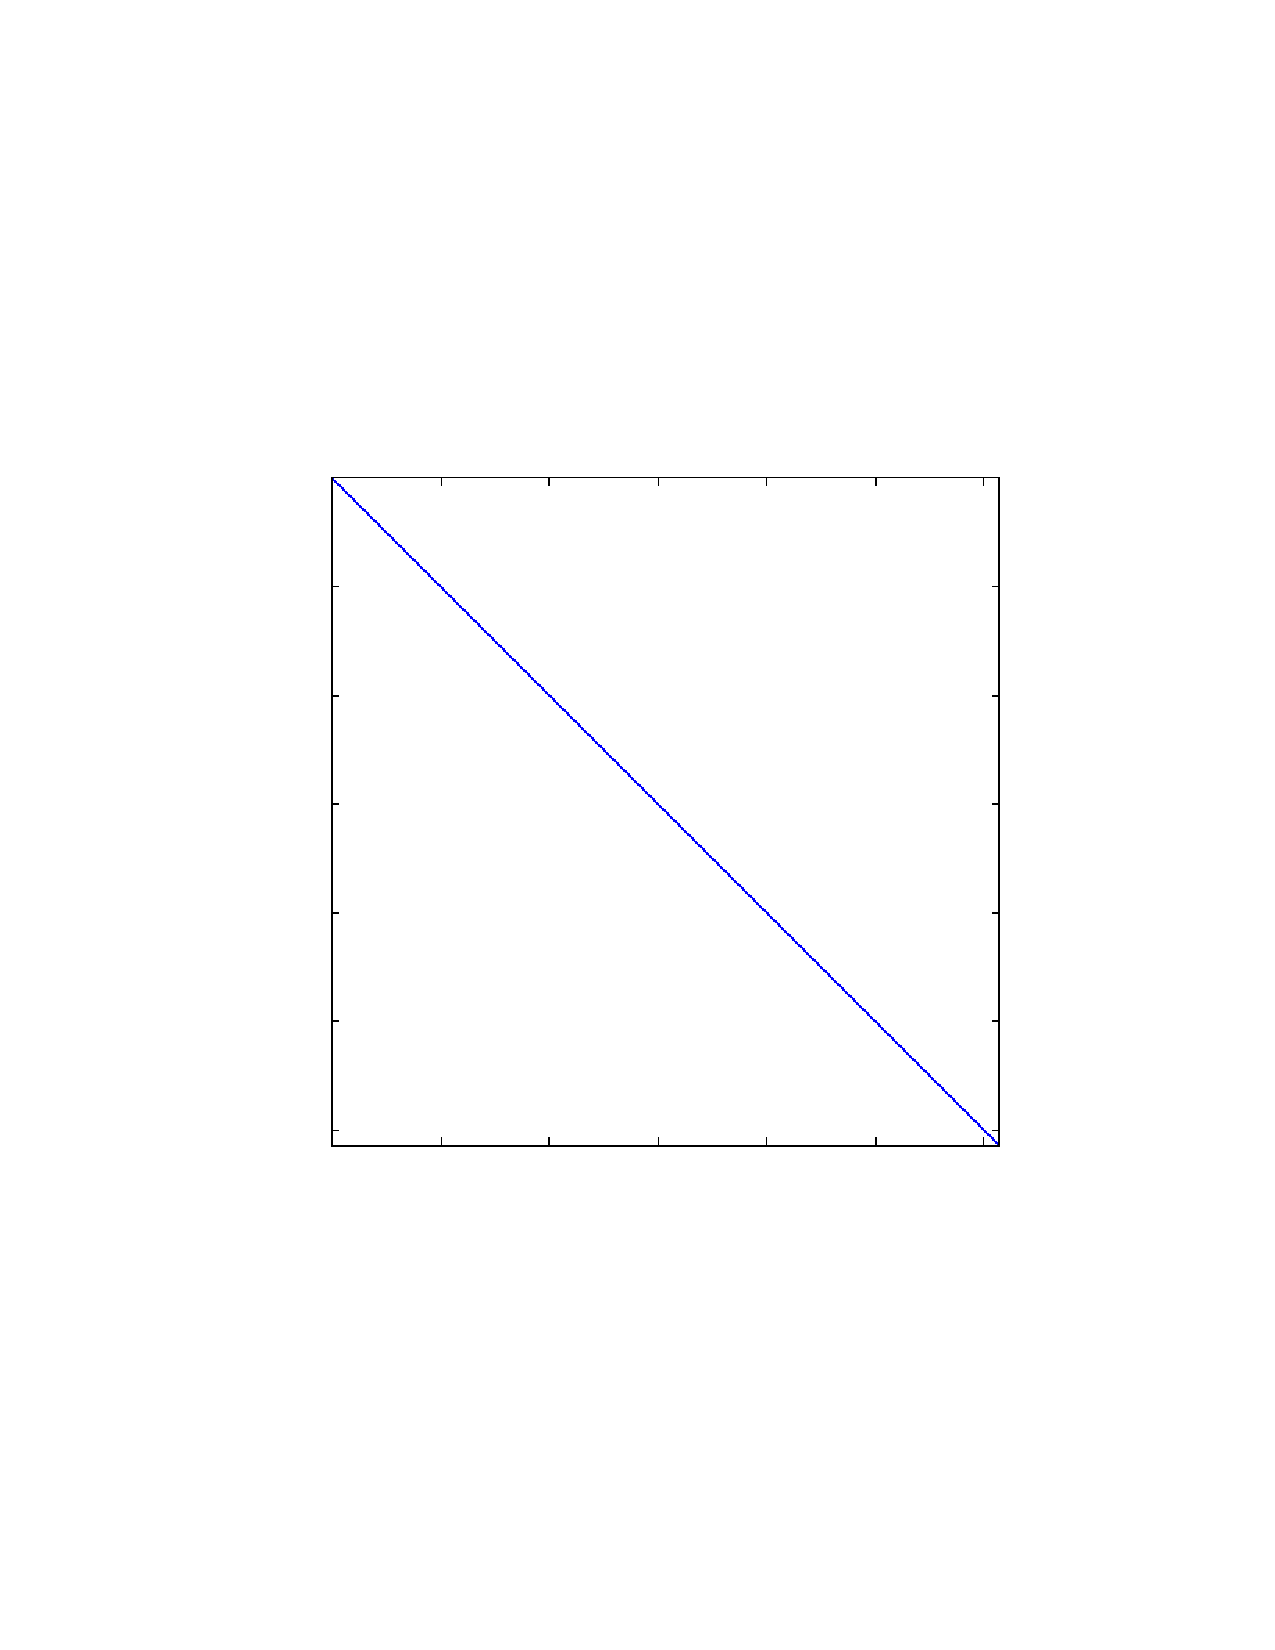
\includegraphics[width=.8in]{FIG6}}
	\hfil
	\subfloat[]{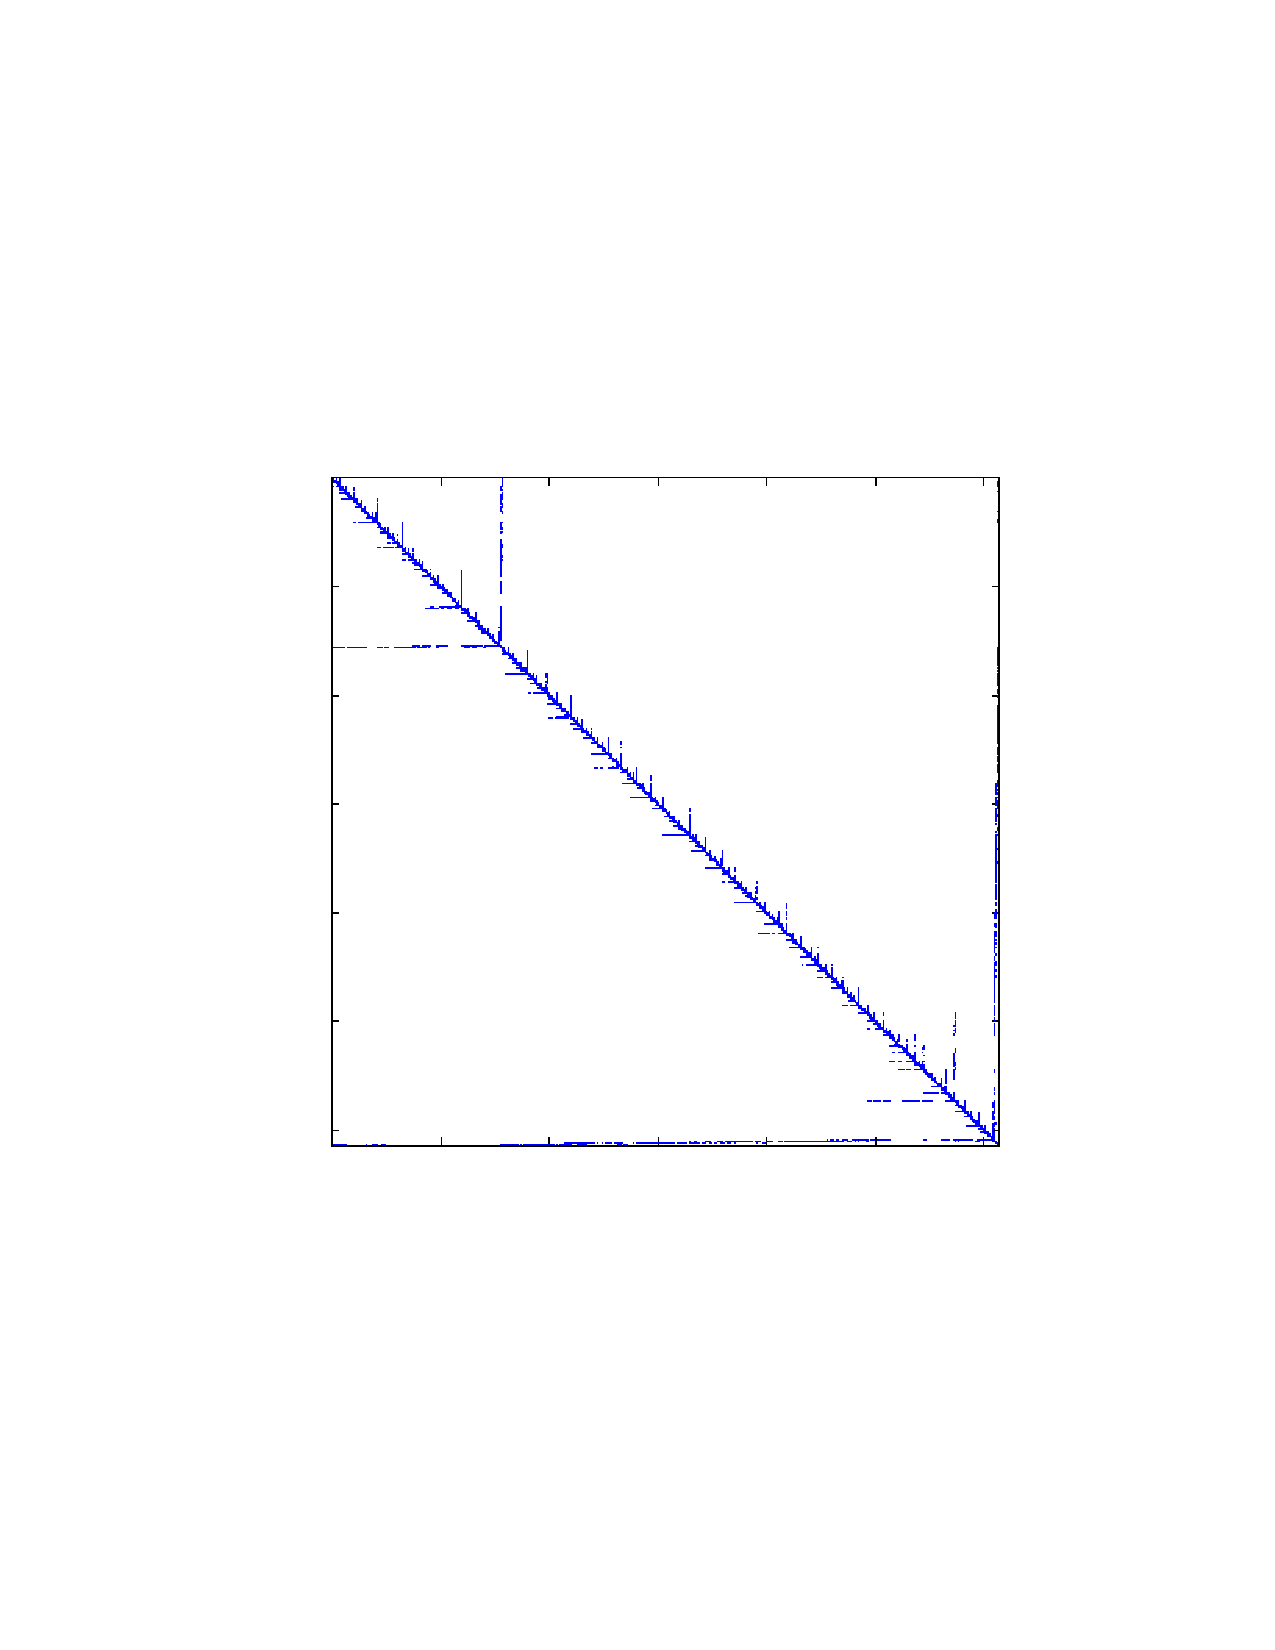
\includegraphics[width=.8in]{FIG7}}
	}
	\caption[The \acrshort{acr:pwgabp} algorithm results using the \acrshort{acr:hus} scheme.]{The \gls{acr:pwgabp} algorithm results using the \gls{acr:hus} scheme for the matrix ``thermal2'. (a) The \gls{acr:hus} parallel iteration increase rate. (b) Sparsity structure of original ''thermal2.`` (c) \gls{acr:rcm} reordered. (d) \gls{acr:amd} reordered.}
	\label{fig:hu-gabp}
\end{figure}


\section{Conclusion}
Implementation-oriented algorithms of \gls{acr:pwgabp} were presented which demonstrated speedups of up 1.8$\times$ over the \gls{acr:dpcg} algorithm.
Also, both improvements in execution time and reduction in iteration count over the \gls{acr:dpcg} solver were demonstrated using the \gls{acr:pwgabp} algorithm with the \gls{acr:sus} scheme.
While the \gls{acr:pwgabp} solver demonstrated an advantage over the \gls{acr:dpcg} solver for \gls{acr:sdd} matrices, the performance for more general \gls{acr:fem} matrices is clearly not competitive against leading solvers such as \gls{acr:icpcg} or multigrid; nonetheless, this study provides valuable insights for the later development and implementation of the \gls{acr:fgabp} and the \gls{acr:fmgabp} algorithms presented in Chapters \ref{chp:FGaBP} and \ref{chp:FMGaBP} which fix the convergence rate issue.
The \gls{acr:hus} algorithm was introduced and its implementation demonstrated enhanced parallel performance for \gls{acr:pwgabp}.
The \gls{acr:hus} algorithm results showed considerable reductions in parallel iterations demonstrating great potential for efficient implementations on CPU-clusters and many-core \gls{acr:hpc} platforms.

%==========
\graphicspath{{./figs/Chp-RelGaBP/}}


%%Fakesection Acronym reset
\glsreset{acr:rgabp}
\glsreset{acr:drgabp}
\glsreset{acr:sdd}
\glsreset{acr:wdd}


\chapter{Relaxed Gaussian Belief Propagation}
\label{chp:relGaBP}
%%Fakesection Abstract
The solution developed in this chapter is motivated by the fact that the \gls{acr:pwgabp} solver requires a large number of iterations to converge if the sparse matrix is \gls{acr:wdd} or is ill-conditioned.
Such matrices can arise from many application domains including the \gls{acr:fem}.
In this work, we present a relaxed form of \gls{acr:pwgabp} that reduces the number of iterations, resulting in significant computational reduction (up to 12.7$\times$) for ill-conditioned large linear systems.
In addition, to circumvent the need of determining the relaxation factor for the new algorithm a priori, we propose a second algorithm that incrementally determines a suitable relaxation factor based on iterative error improvements that also results in similar reductions in \gls{acr:pwgabp} iterations.
We show that the new algorithms can be implemented without any significant increase, over the original \gls{acr:pwgabp}, in both the computational complexity and the memory requirements.
We demonstrate the advantages of our algorithms using empirical results of large, ill-conditioned, and \gls{acr:wdd} matrices.


\section{Introduction}

\gls{acr:pwgabp} was empirically found to exhibit fast convergence for problems where the inverse covariance matrix of the underlying multivariate Gaussian distribution, or similarity the matrix $A$ of the sparse linear system, is \gls{acr:sdd} \cite{bib:Weiss01CorrectnessBelief, bib:Shental2008GBPSSLE}, especially when compared to the \gls{acr:dpcg} solver as shown in \chpRef{chp:PW-GaBP}.
However, if $A$ is large, sparse and ill-conditioned, then \gls{acr:pwgabp} may require a large number of iterations.
The work in \cite{bib:Weiss01CorrectnessBelief} provides a rough upper bound on the number of iterations required by \gls{acr:pwgabp} to reach a given convergence tolerance $\epsilon$; however, it is only applicable for \gls{acr:sdd} matrices.
The work in \cite{bib:Shental2008GBPSSLE} uses a common convergence acceleration method referred to as the Aitken-Steffensen's acceleration to speedup the \gls{acr:pwgabp} convergence.
In the Aitken-Steffensen's acceleration scheme, an improved estimate of a message is computed at each third iteration as:
\begin{equation}
	m\approx \hat{m}^{(t)}=m^{(t-3)}-\frac{(m^{(t-2)}-m^{(t-3)})^{2}}{m^{(t-1)}-2m^{(t-2)}+m^{(t-3)}}
\end{equation}
where $m^{(t)}$ represents a message estimate at iteration $t$. 
However, when this acceleration is used in \gls{acr:pwgabp} with ill-conditioned matrices, it yields unstable results even with double-precision implementations.
In addition, this acceleration scheme requires the additional storage of prior iteration messages which makes it very costly when implemented for large problems.


In this study, we will consider ill-conditioned matrices that are not necessarily \gls{acr:sdd}, which require considerably larger number of \gls{acr:pwgabp} iterations.
Finding a theoretical upper bound for the convergence rate of \gls{acr:pwgabp} for such matrices is still an open research question.
In addition, some of the solutions developed in this chapter are not only applicable to \glspl{acr:pwgm} but, rather, can also be used for general \glspl{acr:gm} such as the ones developed for the \gls{acr:fem} problem as will be illustrated in \chpRef{chp:FGaBP}.
However, since in this chapter the numerical analyses of the new solution were all performed in comparison with the original \gls{acr:pwgabp}, we will present the new formulation as an extension of the \gls{acr:pwgabp} solver.


This chapter is organized as follows.
In \secRef{sec:rgabp}, we present the new relaxation scheme for the \gls{acr:pwgabp} algorithm.
\secRef{sec:argabp} presents the dynamic relaxation algorithm.
Finally, in \secRef{sec:argabpResults} we present the numerical results and concluding remarks.


\section{The Relaxed PW-GaBP Algorithm}
\label{sec:rgabp}


In this section we will detail the relaxation formulation of the \gls{acr:pwgabp} algorithm, which was previously presented in the background chapter in \secRef{sec:pwgabp}.
We will proceed with our discussion whereby all the information available from the underlying problem is the matrix $A$.
In addition, we consider matrices that are large, sparse, ill-conditioned, and \gls{acr:wdd}.
With such matrices, the original \gls{acr:pwgabp} algorithm is known to require a very large number of iterations to converge.


\subsection{Edge Message Relaxation}


As can be seen from (\ref{eqn_a_i_minus_j_bc}), (\ref{eqn_b_i_minus_j_bc}) and (\ref{eqn_x_i}), the marginal mean of node $i$, which is also the solution estimate of $U_i^{(t)}$ at iteration $t$, can be obtained using the two sums $\alpha_i^{(t)}$ and $\beta_i^{(t)}$ of messages received on all connected edges $\mathcal{N}(i)$.
It can also be noted from these equations that applying any relaxation on the $\beta$ messages does not affect the $\alpha$ messages convergence properties.  Relaxation on $\beta_{ij}$ can be applied as follows:
\begin{equation}
	\hat{\beta}_{ij}^{(t)} = \gamma \beta_{ij}^{(t)} + (1-\gamma)\beta_{ij}^{(t-1)}
\end{equation}
where $\gamma$ is referred to as the relaxation factor.
The relaxation factor $\gamma$ is obtained from the limit  $\gamma \in [0,2]$.
If $\gamma$ is in $[0,1]$, the method is referred to as under-relaxation or damping and, in certain cases, is used to force a divergent \gls{acr:pwgabp} to converge at the expense of a high iteration count.
If $\gamma $ is in $[1,2]$, the method is referred to as over-relaxation and is used to accelerate convergence, which is the objective of this work.  
The new relaxed message $\hat{\beta}_{ij}^{(t)}$ can be communicated instead of $\beta_{ij}^{(t)}$.
It can be seen that if $\gamma$ is chosen such that the \gls{acr:pwgabp} algorithm is convergent, the relaxed messages converge as $\beta_{ij}^{(t)} \approx \beta_{ij}^{(t-1)}$.
This indicates that the stationarity point of the relaxed algorithm is that of the original \gls{acr:pwgabp}.
We refer to this style of relaxation as \gls{acr:emr}.
It is clear that this relaxation does not require additional memory since it only requires the previous iteration message.
The \gls{acr:emr} relaxation is the most flexible and can be applied to any \gls{acr:gm}.


\subsection{Nodal Message Relaxation}


An alternative strategy to \gls{acr:emr}, we can apply relaxation to the nodal sum $\beta_i$ messages as opposed to each individual edge message $\beta_{ij}$.
The $\beta_i$ messages are then relaxed as follows:
\begin{equation}
	\hat{\beta}_{i}^{(t)} = \gamma \beta_{i}^{(t)} + (1-\gamma)\beta_{i}^{(t-1)} \label{eq_relx_b_i}.
\end{equation}
We refer to this relaxation scheme as the \gls{acr:nmr}.
Relaxing $\beta_i$ messages requires additional memory of order $\bigo{N}$ to store the previous iteration's $\beta_{i}^{(t-1)}$ value.
However, based on the distinct observation that for every matrix we tested from the class of \gls{acr:wdd} matrices, the $\alpha$ messages converged much faster than the $\beta$ messages to within 10 to 20 iterations as demonstrated by our empirical results.
If we decide to use this property, we can eliminate the additional memory requirement due to relaxing $\beta_i$ messages by reformulating the updates as follows: 
\begin{align}
	\hat{\beta}_{i}^{(t+t_{o})} & =  \alpha_{i}^{*}\hat{\mu}_{i}^{(t+t_{o})}  \\
	\intertext{where:}
	\hat{\mu}_{i}^{(t+t_{o})} & =  \gamma \mu_{i}^{(t+t_{o})}+(1-\gamma)\mu_{i}^{(t+t_{o}-1)} \label{eq_relx_x_i}
\end{align}
where $\alpha_i^*$ is the fixed point reached after $t_o$ iterations.
The $\mu_{i}^{(t-1)}$ values are reused here since they are used to store the final solution.

To illustrate the correctness of the \gls{acr:nmr} based on the original \gls{acr:pwgabp} update rules of $\beta_{ij}$ messages, we substitute (\ref{eq_relx_b_i}) into (\ref{eqn_b_i_minus_j_bc}) and then into (\ref{eqn_GaBPUpdateM}) to obtain the following:
\begin{align}
	\hat{\beta}_{ij}^{(t+t_{o})} & = \frac{-A_{ij}}{\alpha_{i\setminus j}^{*}}\hat{\beta}_{i\setminus j}^{(t+t_{o})}\\
	\intertext{where,}
	\hat{\beta}_{i\setminus j}^{(t+t_{o})} & = \hat{\beta}_{i}^{(t+t_{o})}-\beta_{ji}^{(t+t_{o})}\\ 
	\begin{split}
		& = \gamma\beta_{i\setminus j}^{(t+t_{o})}+(1-\gamma)\beta_{i\setminus j}^{(t+t_{o}-1)} \\  
		& \quad -(1-\gamma)\Delta\beta_{ji}^{(t+t_{o})}
	\end{split}
	\intertext{and,}
	\Delta\beta_{ji}^{(t+t_{o})} &= \beta_{ji}^{(t+t_{o})} - \beta_{ji}^{(t+t_{o}-1)}.
\end{align}
It can be seen from the above modified \gls{acr:bp} rule for $\beta_{ij}$ messages that if $\gamma$ is chosen such that the relaxed \gls{acr:pwgabp} is convergent, the additional terms $ \Delta\beta_{ji}^{(t+t_{o})}, \forall j $ will approach zero and the relaxed algorithm's fixed point will be equal to the fixed point solution of the original \gls{acr:pwgabp} algorithm.
The listing of the relaxed \gls{acr:pwgabp} algorithm is shown in \algRef{alg:relaxed_gabp}. 
We refer to this algorithm as the \gls{acr:rgabp} algorithm.

\begin{algorithm}[h]
	\centering
	\begin{algorithmic}[1]
		\STATE \textit{Initialize: $\forall i,j$}\\
%\setlength{\belowdisplayskip}{0pt}
%\setlength{\abovedisplayskip}{0pt}
%\begin{align*}
		\begin{tabular}{cc}
			$\alpha_{ij} = 0$ & $ \beta_{ij} = 0$\\ 
			$\gamma \in [1,2]$ & $u_i^{(0)} = 0$
		\end{tabular}
%\end{align*}
		\REPEAT[Start \gls{acr:pwgabp} iteration: $t=1,2,\cdots$]
		\FOR{ each node $i$ }
		\STATE $\alpha_{i} = A_{ii} + \sum_{k \in N(i)} \alpha_{ki}$
		\STATE $\beta_{i} = b_{i} + \sum_{k \in N(i)} \beta_{ki}$
		\IF{$ \frac{\parallel \Delta\alpha_i \parallel}{\parallel \alpha \parallel} < \epsilon\; \forall i$}\label{test}
		\STATE $\hat\beta_i = \gamma\beta_i + (1-\gamma)\alpha_i \mu_i^{(t-1)}$ \COMMENT{Relaxation using $\gamma$} 
		\ELSE
		\STATE $\hat\beta_i = \beta_i$ 
		\AlgENDIF
		\STATE $\mu_i = \hat{\beta}_i / \alpha_i$
		\STATE \COMMENT{Message update subject to a schedule}
		\FOR{ each edge $i \rightarrow j$ } 
		\STATE $\alpha_{ij} = -A_{ij}^2 (\alpha_{i}-\alpha_{ji})^{-1} $
		\STATE $\beta_{ij} = -A_{ij} ( \hat\beta_{i}-\beta_{ji})(\alpha_{i}-\alpha_{ji})^{-1} $
		\AlgENDFOR
		\AlgENDFOR
		\STATE Compute:  $e_r = \left(\frac{\sum (\mu_i - \mu_i^{(t-1)})^2} {\sum \mu_i^2} \right)^{\frac{1}{2}}$
		\UNTIL{Convergence check: $e_r < \epsilon$ }
		\STATE \textit{Output:} $\overline{u} = \left[ \mu_i \right] \forall i$
	\end{algorithmic}
	\caption{The \acrshort{acr:rgabp} algorithm.}
	\label{alg:relaxed_gabp}
\end{algorithm}

The condition for variance convergence in step-\ref{test} of \algRef{alg:relaxed_gabp} is not inherently required but rather is used to reduce the memory requirement.
As explained earlier, once the variances converge, we can obtain $ \beta_i^{(t-1)}$ from $u_i^{(t-1)}$ in order to relax $\beta_i^{(t)}$ which saves implementation memory of up to $O \left( N \right)$.  

By using an over-relaxation factor $\gamma \in [1,2]$, our empirical results indicate that the optimal $\gamma_\mathit{opt}$ that yields the lowest iteration count for a given tolerance ($\epsilon$) for the relative norm, as defined in \secRef{sec:convtest}, depends strongly on the elements of the matrix $A$, which makes $\gamma_\mathit{opt}$ dependent on the underlying problem.
Hence, finding a suitable $\gamma$ may prove difficult especially since using the wrong value will cause the algorithm to fail to converge.
In the following section, we propose a heuristic algorithm that iteratively and incrementally finds an approximation to $\gamma$ that, in general, produces a sufficiently fast convergence by iteratively reducing the relative norm.


\section{Dynamic Over-relaxation}
\label{sec:argabp}

The solution presented here, which circumvents determining $\gamma_{opt}$ a priori, is motivated by the following empirical observations of the \gls{acr:rgabp} algorithm: a threshold $\gamma_\mathit{opt}$ exists in the interval $[1,2]$ that is also found to be a maximum in the same interval for given initial conditions, any further increase in $\gamma_{opt}$ will cause a substantial increase in $ e_r^{(t)}$.
As a result, we can propose a dynamic update scheme for $\gamma$ based on the progress of the \gls{acr:rgabp} relative norm.
More precisely, we can gradually increase $\gamma$ starting from an initial value by adding an increment $\Delta\gamma$ each $d$ number of iterations as long as the $e_r$ is improving.
However, if $e_r$ is found not to improve, we can likewise decrement $\gamma$.
\algRef{alg:gamma_update} shows the details of an algorithm that can be used to find a rough estimate of the over-relaxation $\gamma$ which results in a high relative norm decrease rate. 


\begin{algorithm}[h]
	\centering
	\begin{algorithmic}[1]
		\STATE \textit{Initialize:}\\
		\begin{tabular}{ll}
			$e_\mathit{best} = 1.0$ & $\gamma^{(0)}  = 1.0$\\ 
			$d  = 10$ & $\Delta\gamma  = 0.1$
		\end{tabular}
		\REPEAT[\gls{acr:pwgabp} iteration: $t=1,2,\cdots$]
		\IF{$ t\mod{d} = 0$}
		\IF{$e_r^{(t)} < e_\mathit{best}$}
		\STATE $\gamma^{(t)} = \gamma^{(t-1)} + \Delta\gamma$ \COMMENT {Increment $\gamma$}
		\STATE $e_\mathit{best} = e_r^{(t)}$
		\ELSE
		\STATE $\gamma^{(t)} = \gamma^{(t-1)} - \Delta\gamma$ \COMMENT{Decrement $\gamma$}
		\IF{$\gamma^{(t)} < 1.0$}
		\STATE $\gamma^{(t)} = 1.0$
	\ENDIF
\ENDIF
\ENDIF
\UNTIL{\gls{acr:pwgabp} terminates }
\end{algorithmic}
\caption{The \gls{acr:drgabp} algorithm.}
\label{alg:gamma_update}
\end{algorithm}


\algRef{alg:gamma_update} relies on two basic settings $\Delta \gamma$ and $d$.
The parameter $\Delta \gamma$ is a fixed increment or decrement size which nominally can be set to $0.1$, while $d$ is the iteration interval length on which $e_r$ can be tested in order to adjust $\gamma$.
The relative norm sampling interval $d$ should be chosen wide enough so that the fluctuations in $e_r$, resulting from the prior $\gamma$ change, can diminish resulting in a stable value for $e_r$ that can be sampled.
In all of the cases we analyzed for ill-conditioned \gls{acr:wdd} matrices, a good value for $d$ was found to be around 10 to 20 iterations.
We refer to this algorithm as the \gls{acr:drgabp} algorithm.


If $\Delta\gamma$ is chosen sufficiently small with a sufficiently wide relative norm sampling iteration interval $d$, the \gls{acr:drgabp} algorithm should converge.
Unlike the Aitken-Steffensen or similar acceleration methods, this algorithm is computationally more stable specially for ill-conditioned matrices.
Another key advantage of the \gls{acr:drgabp} algorithm is that it does not require a significant increase in both computation and memory over the original \gls{acr:pwgabp} algorithm. 


\section{Results and Discussions}
\label{sec:argabpResults}

The test matrices are obtained from the classical L-shaped conductor problem in electromagnetics.
As shown in \figRef{fig:L-shaped}, the potential in the space between the two square conductors carrying different voltages is found by solving the Laplace equation, $ \nabla^2 u = 0 $.
However in practice, Laplace's equation is solved numerically by the \gls{acr:fem}, which starts by dividing the interconductor space into triangular elements.
Using a first order \gls{acr:fem},  the problem typically requires the solution of a linear system of equations that is large, sparse, ill-conditioned, and \gls{acr:wdd}.
In this section, we demonstrate the effectiveness of our developed algorithms, the \gls{acr:rgabp} and the \gls{acr:drgabp}, by solving the linear system arising from this Laplace problem.
We also use a selected set of other generated matrices in order to illustrate our empirical results.
We used asynchronous message scheduling for all our algorithms.
The relative norm $e_r$ is recorded at each iteration.
All algorithms were terminated when the normalized residual ($l^2$-norm) reached $R < 10^{-9}$.

\begin{figure}[h]
	\centerline{
	\subfloat[]{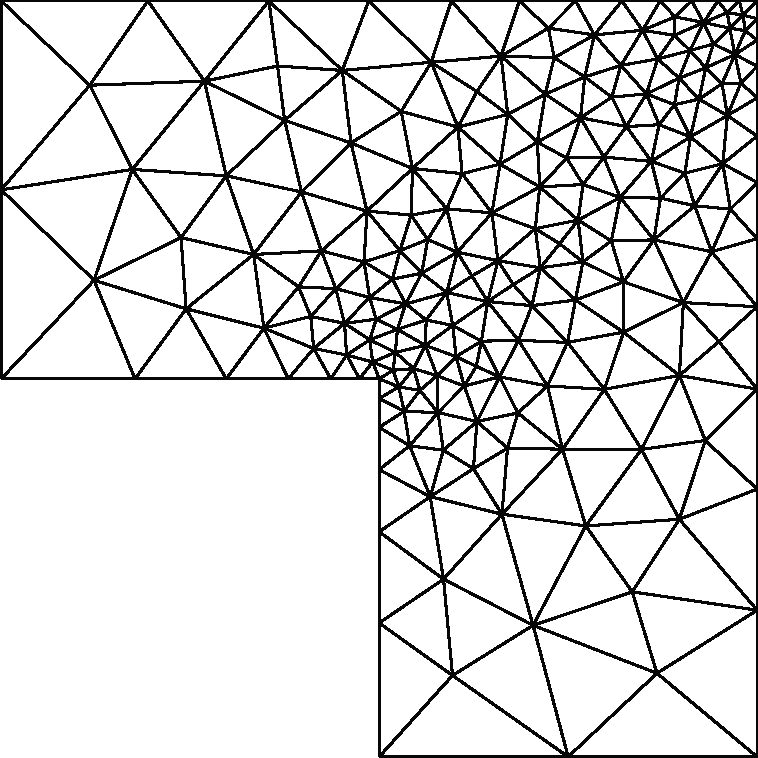
\includegraphics[width=1.75in]{L-shaped}}
	\hspace{2em}
	\subfloat[]{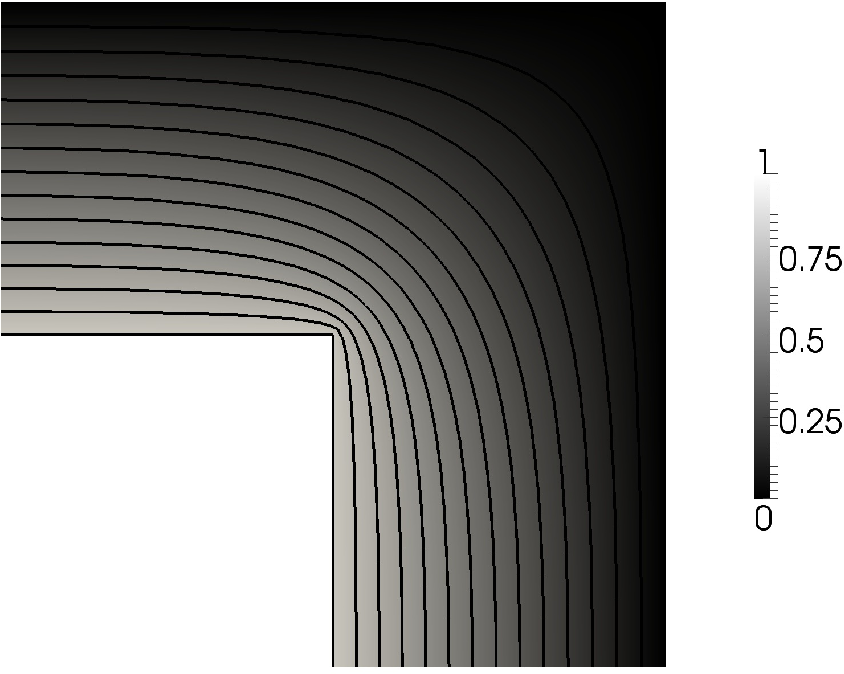
\includegraphics[width=2.2in]{L-shaped_sol}}
	}
	\caption[The L-shaped conductor problem.]{L-shaped conductor problem of dimensions equal to 1cm. (a) Illustrated discretization using a small mesh. (b) Equipotential lines of the potential solution of the Laplace's equation, volts scale.}
	\label{fig:L-shaped}
\end{figure}

The plots in \figRef{fig:err_rlx} demonstrate the iteration reduction due to the \gls{acr:rgabp} algorithm.
The  size of the linear system characterized by the matrix $A$ is $N=2700$ unknowns, with number of non-zeros $\gls{acr:nnz} = 17572$.
The original \gls{acr:pwgabp} algorithm required 2449 iterations while the \gls{acr:rgabp} algorithm required as low as 389 iterations for $\gamma = 1.538$ resulting in a reduction factor of 6.2.
It can be observed that the overall relative norm decreases consistently as $\gamma$ increases to a certain value in the interval $[1,2]$.
It is expected that for this problem the best $\gamma_\mathit{opt}$ can be empirically obtained as $\gamma_\mathit{opt} \approx 1.538$, any further increase on $\gamma$ will cause $e_r$ to increase, and consequently causing the algorithm to fail to converge.


\begin{figure}[h]
	\centering
	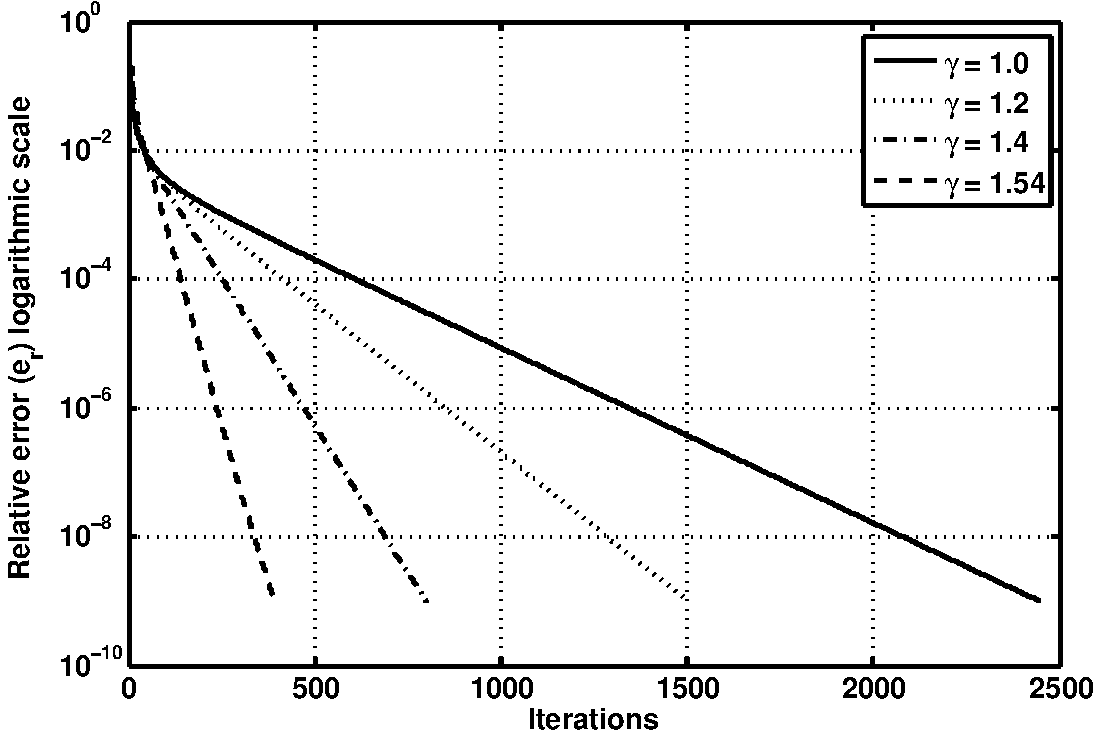
\includegraphics[width=4in]{err_plot_1}
	\caption[Performance of the \acrshort{acr:rgabp} for different relaxation factors.]{The relative norm $e_r$ plots for the \gls{acr:rgabp} algorithm with different relaxation factors $\gamma$.}
	\label{fig:err_rlx}
\end{figure}

The plots in \figRef{fig:err_IncRlx} show the results of the \gls{acr:drgabp} algorithm in obtaining a considerably lower \gls{acr:pwgabp} iteration count without prior knowledge of $\gamma_{opt}$.
The parameter $\Delta\gamma$ is varied from the fine value of $10^{-2}$ to the coarser value of $2\times 10^{-1}$.
A relative norm sampling interval of $d = 10$ was used for all plots.
It is worth noting here that the best iteration reduction was found for $\Delta\gamma = 2\times 10^{-1}$ resulting in 337 iterations.
This is lower than the previously reported 389 iterations by \gls{acr:rgabp} assuming prior knowledge of $\gamma_{opt}$.
This reduction may be attributed to the dynamics of the algorithm in alternating between two values of $\gamma$ which are (1.3 and 1.6). 

\begin{figure}[h]
	\centering
	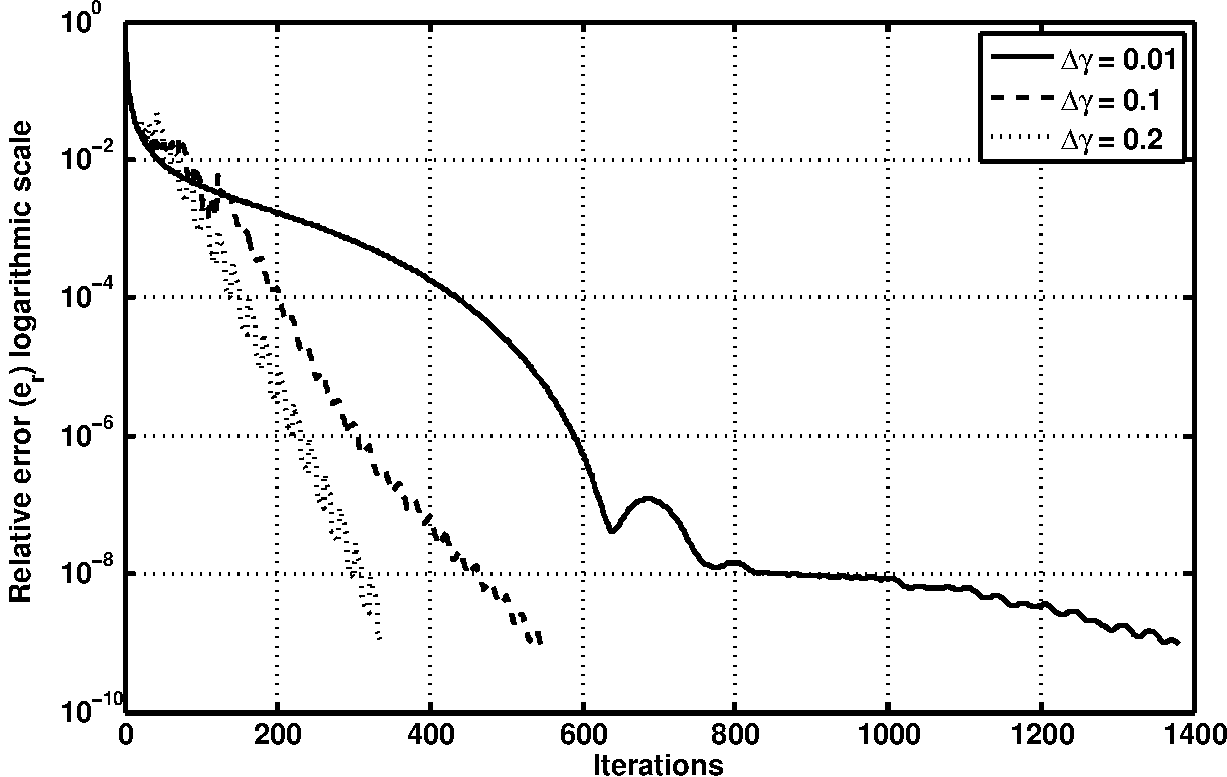
\includegraphics[width=4in]{err_plot_2}
	\caption[Performance of \acrshort{acr:drgabp} for different relaxation increments.]{The relative norm $e_r$ plots for the \gls{acr:drgabp} algorithm with different relaxation increments $\Delta\gamma$.}
	\label{fig:err_IncRlx}
\end{figure}

The case of \gls{acr:drgabp} with $\Delta\gamma = 10^{-2}$ resulted in 1381 iterations.
While this performance is still considerably better than the original \gls{acr:pwgabp}, the larger comparative iterations may be attributed to the fact that $\gamma$ fluctuates between two values which do not necessarily produce the lowest overall relative norm.
However, the algorithm converged for all considered values of $\Delta\gamma$.
In general, the smaller the values of $\Delta\gamma$ are, the wider the applicability of the algorithm at the expense of a higher iteration count.
We found that the nominal $\Delta\gamma = 10^{-1}$ is suitable for most matrices that are ill-conditioned and weakly diagonally dominant.   


We illustrate in \tableRef{tbl:testmatrices_RGaBP} a selected set of test matrices.
One matrix was obtained from the Matrix Market website repository \cite{bib:matrixMarket}.
The other two matrices were generated randomly using Matlab and set to be sparse and \gls{acr:wdd}.
The generated matrices all have negative off-diagonals which results in ill-conditioned matrices.
For all algorithms we used $d = 10$.
The variances for all matrices converged in less than 10 iterations.
The density \% of the matrix is measured by $\gls{acr:nnz} / N^2 \times 100$.

\tableRef{tbl:testmatrices_RGaBP} demonstrates that reductions in iterations were produced by the \gls{acr:rgabp} algorithm in all test cases.
The second matrix shows a reduction factor of 12.7 for $ \gamma = 1.8 $.
\tableRef{tbl:testmatrices_DRGaBP} shows the results of \gls{acr:drgabp} which also produced significant iteration reductions versus the original \gls{acr:pwgabp}.
The performance of \gls{acr:drgabp} algorithm can depend on the choice of $\Delta\gamma$, however the algorithm converged in all tested cases.
It was observed that the nominal value of $\Delta\gamma = 0.1$ resulted in best reductions on average.

\begin{table}[h]
	\centering
	\begin{threeparttable}[c]
		\caption{Results for the \acrshort{acr:rgabp} algorithm on selected test matrices.}
		\label{tbl:testmatrices_RGaBP}
		\begin{tabular}{ccccccc}
			\toprule
			\multirow{2}{*}{Matrix} & \multirow{2}{*}{N} & Density & \multirow{2}{*}{\gls{acr:pwgabp}} & \multicolumn{2}{c}{R-GaB} & Red.\tabularnewline
			\cline{5-6} 
			&  & (\%) &  & Itrs & $\gamma$ & Factor\tabularnewline
			\midrule 
			gr\_30\_30 \cite{bib:matrixMarket} & 900 & 0.956 & 859 & 115 & 1.59 & 7.5\tabularnewline
			Sp Rand 1 & 5000 & 0.4 & 5571 & 437 & 1.8 & 12.7\tabularnewline
			Sp Rand 2 & 3000 & 0.4 & 3028 & 241 & 1.67 & 12.6\tabularnewline
			\bottomrule
		\end{tabular}
	\end{threeparttable}
\end{table}


\begin{table}[h]
	\centering
	\begin{threeparttable}[c]
		\caption{Results for the \acrshort{acr:drgabp} algorithm on selected test matrices.}
		\label{tbl:testmatrices_DRGaBP}
		\centering
		\begin{tabular}{ccccc}
			\toprule
			\multirow{2}{*}{Matrix} & \multicolumn{3}{c}{\gls{acr:drgabp}} & Red. Factor\tabularnewline
			\cline{2-4} 
			& $\Delta\gamma=0.01$ & $\Delta\gamma=0.1$ & $\Delta\gamma=0.2$ & $\Delta\gamma=0.1$\tabularnewline
			\midrule 
			gr\_30\_30 \cite{bib:matrixMarket} & 456 & 783 & 647 & 1.1\tabularnewline
			Sp Rand 1 & 1873 & 872 & 1492 & 6.4\tabularnewline
			Sp Rand 2 & 732 & 759 & 963 & 4.0\tabularnewline
			\bottomrule
		\end{tabular}
	\end{threeparttable}
\end{table}


\section{Conclusion}
We have presented the \gls{acr:rgabp} algorithm which implements new relaxation schemes for the \gls{acr:pwgabp} algorithm to considerably accelerate its convergence for ill-conditioned \gls{acr:wdd} inverse covariance matrices.
We have demonstrated empirical reductions in iterations of up to 12.7 times.
We have also introduced the \gls{acr:drgabp} algorithm that avoids the complexity of setting a prior over-relaxation factor.
The \gls{acr:drgabp} algorithm demonstrates performance comparable with the \gls{acr:rgabp} algorithm with a prior knowledge of an optimal relaxation factor.
The new algorithms do not require any increase of the computational complexity or the memory requirements of the original \gls{acr:pwgabp} algorithm hence facilitating efficient implementations on parallel architectures.



%==========
\graphicspath{{figs/Chp-FGaBP/}}


%%Fakesection Acronym reset
\glsreset{acr:fg}
\glsreset{acr:gm}
\glsreset{acr:bp}
\glsreset{acr:fgabp}
\glsreset{acr:femfg}
\glsreset{acr:ca}
\glsreset{acr:aufgabp}
\glsreset{acr:mgpcg}
\glsreset{acr:pwgabp}
\glsreset{acr:pwgm}
\glsreset{acr:spd}
\glsreset{acr:csr}
\glsreset{acr:dpcg}
\glsreset{acr:nmr}
\glsreset{acr:emr}
\glsreset{acr:su}
\glsreset{acr:ssc}

\chapter{Parallel Solution of the Finite Element Method Using Gaussian Belief Propagation}
\label{chp:FGaBP}

%%Fakesection From abstract
The proliferation of parallel architectures such as manycore CPUs and GPUs drives the need to redesign conventional algorithms with parallelism in mind.
However, the parallel performance of conventional \gls{acr:fem} implementations can be limited by the inherent coupling of the underlying sparse data-structures.
In this chapter, we look into \gls{acr:bp} inference algorithms to address these challenges.
We introduce a probabilistic \gls{acr:gm} of the \gls{acr:fem} based on \glspl{acr:fg} by recasting the global deterministic \gls{acr:fem} as a localized variational inference problem.
The resulting algorithm eliminates the need to assemble any global sparse data-structure or perform any global sparse algebraic operation.


\section{Introduction}
\label{sec:gabpIntro}
%From Introduction section
We have presented in \secRef{sec:pwgabp} a background of the \gls{acr:pwgabp} algorithm and showed that it is a recursive message passing algorithm that offers distributed computations \cite{bib:Pearl88ProbabilisticReasoning, bib:Weiss01CorrectnessBelief, bib:Shental2008GBPSSLE}.
\gls{acr:pwgabp} demonstrated better empirical results than conventional iterative solvers such as Jacobbi, \gls{acr:gs}, \gls{acr:sor} and \gls{acr:dpcg} for \gls{acr:sdd} matrices \cite{bib:El-Kurdi2012EIOGBPSFLSDDLS, bib:Shental2008GBPSSLE, bib:El-Kurdi2012RGBP}.
We have also shown in \chpRef{chp:PW-GaBP} that the \gls{acr:pwgabp} algorithm can potentially parallelize \gls{acr:fem} applications when using scheduling schemes that facilitates its parallel execution \cite{bib:El-Kurdi2012RGBP}.
While new schemes were introduced in \chpRef{chp:relGaBP} to accelerate the \gls{acr:pwgabp} for \gls{acr:fem} matrices using the dynamic relaxation \gls{acr:drgabp} algorithm, the overall performance of the \gls{acr:drgabp} algorithm was still short of popular solvers such as the \gls{acr:icpcg} solver.
However, the \gls{acr:pwgabp} solver, and similarly all other conventional solvers, still requires the assembly of a large sparse matrix data-structure.
Many applications that require repeated reassembly of the global matrix, such as adaptive multigrid and non-linear applications, can suffer from the long setup time of the sparse matrix.


We believe that the assembly of the sparse matrix and the algebraic operations on such data-structures are the sources of bottlenecks that are hindering efficient parallel implementations for the \gls{acr:fem} computation on \gls{acr:hpc} platforms.
Novel and inherently parallel algorithms, therefore, need to be developed from a completely different perspective in order to address this issue.
The classical variational formulation of the \gls{acr:fem} provides useful physical insight for the underlying \gls{acr:bvp}, which leads us to exploring the use of a different breed of algorithms used in variational inference such as \gls{acr:bp} \cite{bib:Pearl88ProbabilisticReasoning}.
In this work, we present a new \gls{acr:bp}-based algorithm specifically derived for the \gls{acr:fem} that is referred to as the \gls{acr:fgabp}.
We first develop a variational inference formulation for the \gls{acr:fem} in order to facilitate its interpretation as a \gls{acr:gm} problem.
We then introduce the \gls{acr:fg} model for the variational inference \gls{acr:fem} referred to as the \gls{acr:femfg} model.
Next, we use the new \gls{acr:femfg} model to develop the \gls{acr:fgabp} algorithm.
We show that the \gls{acr:fgabp} algorithm is applicable for arbitrary element geometry and interpolation order, which is needed to address a wide variety of \gls{acr:fem} applications.
The \gls{acr:fgabp} algorithm provides better parallel computations than conventional algebraic methods by avoiding the assembly of the global sparse matrix, and by solving the \gls{acr:fem} in parallel element-by-element without the need to perform any global sparse matrix operations.
The new algorithm provides flexible memory bandwidth utilization due to its use of distributed message-based computations, referred to as message scheduling, which allows us to adapt its implementation on hardware using various memory architectures without impacting the algorithm's computational stability.
Such a critical advantage is usually lost when adapting reformulation techniques of the \gls{acr:cg} solver such as the \gls{acr:ca} \cite[p. 34]{bib:Hoemmen2010EECS} which is based on the $s$-step \cite{bib:Chronopoulos1989153} method.




The chapter is organized as follows.
In \secRef{sec:FEMVI} we present the formulation of the \gls{acr:fem} as a variational inference problem.
In \secRef{sec:FEMFG} we introduce the \gls{acr:femfg} model, and in \secRef{sec:femgabp} we derive \gls{acr:bp} update rules on the \gls{acr:femfg} and present the \gls{acr:fgabp} algorithm.
In \secRef{sec:lowerCompFGaBP} we present reformulations of the \gls{acr:fgabp} algorithm that considerably reduce its computational complexity.
In \secRef{sec:elmMerg} we present the element merge solution that enhances the memory bandwidth utilization of the \gls{acr:fgabp} algorithm.
In \secRef{sec:fgabpImp} we detail implementation analysis for the \gls{acr:fgabp} algorithm.
Finally, in \secRef{sec:fgabpRes} we conclude with our results and discussions illustrating the \gls{acr:fgabp} execution on \gls{acr:fem} problems.


\section{The FEM as a Variational Inference Problem}
\label{sec:FEMVI}


The work in \cite{bib:Yedidia2004CFEAAGBPA,bib:Yedidia2000genbp}, introduced by Yedidia et al., shows that the \gls{acr:bp} solution on \gls{acr:fg} models corresponds to the Bethe approximation of the free energy \cite{bib:Bethe,bib:Kikuchi} associated with the underlying inference model.
Using that insight, we will derive the \gls{acr:fgabp} algorithm to minimize the variational energy of the \gls{acr:fem} problem.
To that end, we first model the \gls{acr:fem} in terms of a probabilistic \gls{acr:gm} referred to as the \gls{acr:fem} Factor Graph (\gls{acr:femfg}).
We start by reformulating the \gls{acr:fem} as a variational inference problem by modifying the \gls{acr:fem} functional \eqnRef{eqn:discFunc} as follows:

\begin{align}
	\mathcal{P}(U) & = \frac{1}{Z} \exp\left[ -  \sum_{s\in\mathcal{S}}\mathcal{F}_s(U_s) \right] \label{eqn:gpf}\\
	& = \frac{1}{Z} \prod_{s \in \mathcal{S}} \Psi_s(U_s) \label{eqn:fgpf}
\end{align}
where $Z$ is a normalizing constant and $\Psi_s(U_s)$ are local factor functions of the local finite element variables $U_s$ defined as:
\begin{equation}
	\Psi_s(U_s) = \exp\left[ -\frac{1}{2} U^T_s M_s U_s +B_s^T U_s\right]. \label{eqn:Psi}
\end{equation}
It is worth noting that $\Psi_s$ as defined in (\ref{eqn:Psi}) takes a multivariate Gaussian form albeit unnormalized when the element characteristic matrix $M_s$ is \gls{acr:spd}.
\appRef{app:gaDiss} presents more details about Gaussian distributions and their properties.

It can be shown that $\mathcal{P}$ as in (\ref{eqn:gpf}) represents a Gaussian multivariate probability distribution when $\mathcal{F}$ is convex quadratic \cite{bib:Wainwright2008GMEFAVI}.  Hence, the optimality condition of $\mathcal{F}$ can be restated as:
\begin{equation}
	\argmin_{U} \mathcal{F} = \argmax_{U} \mathcal{P}. \label{eqn:statPoint}
\end{equation}
Here, we assume that the variables vector $U$ will represent joint Gaussian random variables under the distribution $\mathcal{P}$.
Since $\mathcal{P}$ is maximized when $U = \mu$, where $\mu$ is the mean vector of $\mathcal{P}$, the \gls{acr:fem} minimization problem of the functional $\mathcal{F}$ is transformed into a computational inference problem of finding the marginal means of the random variables $U$ under the distribution $\mathcal{P}$.
Hence, \gls{acr:bp} inference algorithms can be employed to compute the marginal means of the random variables $U$.

Now, we turn our attention to the normalizing constant $Z$ in \eqnRef{eqn:gpf}.
Wainright and Jordan have presented a framework for variational inference on exponential distributions in \cite{bib:Wainwright2008GMEFAVI}.
We will follow a similar approach to analyze the distribution $\mathcal{P}$.
In our case, $Z$ ensures that $\mathcal{P}$ is a valid distribution such that:
\begin{equation}
	\int_U \mathcal{P}\, \mathrm{d} U = 1
\end{equation}
or alternatively:
\begin{equation}
	Z(M_s,B_s) = \int_U \exp \left( \mathcal{-F} \right)\, \mathrm{d} U <+\infty,\,\,\,\forall s
\end{equation}
that is $Z$ is a function of $M_s$ and $B_s$ such that $Z(M_s,B_s)$ is finite.
Since $\mathcal{F}$ is quadratic, and by convex analysis, finiteness of the integral can be met by ensuring that the element matrices $M_s$ are positive definite.
Observing that $\mathcal{F}$ can also be represented in an assembled form, then the finiteness requirement can alternatively be met by ensuring that the assembled form of the \gls{acr:fem} matrix is positive definite.
Note that the symmetry condition on $M_s$ can be imposed only to simplify the \gls{acr:bp} update rules derivations by assuming Gaussian distributions for the underlying random variables, as will be shown in the following sections.


\section{The FEM Factor Graph Model}
\label{sec:FEMFG}

Given the distribution $\mathcal{P}(U)$, one can define a \gls{acr:gm} to perform computational inference in order to infer the marginal distributions of the random variables in $U$.
A widely used class of \glspl{acr:gm} is the \gls{acr:fg} ~\cite{bib:Kschischang2001FGATSA}, which is a bipartite \gls{acr:gm} that directly represents the factorization of $\mathcal{P}$.
We refer to the \gls{acr:fg} model derived from the distribution $\mathcal{P}$ as the \gls{acr:femfg} model.
The \gls{acr:femfg}, as shown in \figRef{fig:FEM_FG}, includes two types of nodes, a random variable node ($u_i$) representing each node in the unknown vector $U$, and a factor node representing the local factors $\Psi_s$.
An edge is inserted between a variable node $u_i$ and a factor node $\Psi_s$ if $u_i$ is an argument of the local factor $\Psi_s$.
For example, the two element \gls{acr:fem} shown in \figRef{fig:FEM_mesh} can be represented by the probability functional $\mathcal{P}(U)=\Psi_a(u_1,u_2,u_3,u_4,u_5,u_6)\Psi(u_4,u_5,u_6,u_7,u_8,u_9)$.  Likewise, the \gls{acr:femfg} shown in \figRef{fig:FEM_FG} contains two factor nodes labeled \fn{a} and \fn{b} each for $\Psi_a$ and $\Psi_b$ correspondingly.
The node \fn{a} has edges to the variable nodes set $\{u_1,u_2,u_3,u_4,u_5,u_6\}$ that are arguments of $\Psi_a$ and, similarly, the node \fn{b} is connected to variable nodes that are arguments of $\Psi_b$.


The \gls{acr:pwgm}, corresponding to the same mesh, is also provided in \figRef{fig:FEM_PW} for comparison.
As mentioned in \secRef{sec:pwgabp}, the \gls{acr:pwgm} model is used to derive the \gls{acr:pwgabp} algorithm as a solver for linear systems of equations \cite{bib:Shental2008GBPSSLE}.
From that perspective, it may seem that the \gls{acr:pwgabp} algorithm has a greater degree of generality; however, the \gls{acr:pwgabp} has major shortcomings when used for \gls{acr:fem} problems.
Mainly, the \gls{acr:pwgm} does not benefit from the underlying \gls{acr:fem} problem structure; as a result, the number of communication links in the \gls{acr:pwgm} is much higher in comparison to the \gls{acr:femfg} model for certain meshes.
While it may be easy to deduce the structure of the \gls{acr:femfg} model from the underlying \gls{acr:fem} mesh, it is important to note that the number of vertices or edges in a mesh does not necessarily correspond to the number of vertices or edges in a \gls{acr:femfg} model as shown in \figRef{fig:FEM_PW}.
We can illustrate the link reduction advantage of the \gls{acr:femfg} model by counting the links in the same example diagrams.
From the figures, the \gls{acr:femfg} requires 12 links while the \gls{acr:pwgm} requires 27 links for a mesh of two second order triangles.
Similarly, link reductions can also be illustrated considering first order quadrilateral and hexahedral meshes and second order tetrahedral meshes.
In fact, the reduction in the number of links for the \gls{acr:femfg} model progressively increases with the order of the \gls{acr:fem} element.
More detailed analysis on this will be provided later in \secRef{sec:fgabpImp}, where we discuss the implementation details.
First order triangular and tetrahedral meshes are the only case where the \gls{acr:femfg} model will contain more links than the \gls{acr:pwgm}.
To remedy this situation, we provide a solution that lowers the number of links in the \gls{acr:femfg} model for first order triangular and tetrahedral meshes by merging elements that share edges or faces.
The element merging solution is detailed in \secRef{sec:elmMerg}.

\begin{figure}[t]
	\centering{
	\subfloat[]{
	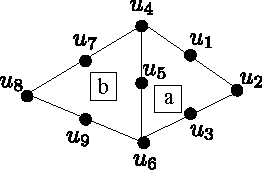
\includegraphics[scale=1.0]{FEM_mesh} \label{fig:FEM_mesh}
	}
  %\hspace{+1mm}
	\subfloat[]{
	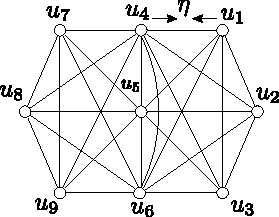
\includegraphics[scale=0.95]{FEM_PW} \label{fig:FEM_PW}
	}
  %\hspace{+2mm}
	\subfloat[]{
	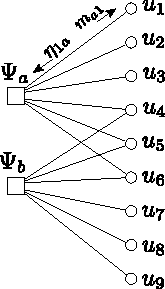
\includegraphics[scale=1.0]{FEM_FG} \label{fig:FEM_FG}
	}
	}
	\caption[Sample \acrshort{acr:femfg}.]{\protect\subref*{fig:FEM_mesh} Sample \gls{acr:fem} mesh of two second order triangles.  Two \gls{acr:gm} representations are shown in \protect\subref*{fig:FEM_PW} and \protect\subref*{fig:FEM_FG}; the messages $\eta$ in a \gls{acr:gm} are communicated recursively either sequentially or in parallel. ~\protect\subref*{fig:FEM_PW}~The conventional \glspl{acr:pwgm}. \protect\subref*{fig:FEM_FG}~The new \gls{acr:femfg} model with reduced number of communication links and improved parallelism.}
	\label{fig:FEM_GM}
\end{figure}



An important remark to make on the \gls{acr:fem} distribution $\mathcal{P}$ is that it is conveniently represented in a factorized form due to its direct derivation from the \gls{acr:fem} functional \eqnRef{eqn:discFunc}.
This factorization reflects the structure of the underlying \gls{acr:fem} mesh that is used to derive the \gls{acr:femfg} model.
In fact, the local factor functions $\Psi_s$ are functions over the cliques in the \gls{acr:pwgm} model representing the sparse matrix we would have obtained, if we chose to assemble the \gls{acr:fem} linear system of equations.
Nonetheless, the term clique is used here for technical convenience since, due to the factorized nature of the exponential distribution $\mathcal{P}$, higher orders of cliques can be formed in the \gls{acr:femfg} model by introducing zero edges in order to form other supersets of cliques.
This can be used, for instance, to improve the memory bandwidth utilization of the algorithm for certain triangular or tetrahedral meshes as later discussed in \secRef{sec:elmMerg}.
This indicates that the \gls{acr:femfg} representation is more adept in exploiting the \gls{acr:fem} problem structure than the \gls{acr:pwgm} representation used for the \gls{acr:pwgabp} solver.
In addition to this flexibility, the \gls{acr:fgabp} algorithm, based on the \gls{acr:femfg} model, demonstrates improved convergence versus the \gls{acr:pwgabp}, as shown later in \secRef{sec:fgabpRes}.
We believe that this improved convergence is a direct consequence of the \gls{acr:femfg} model better exploiting the underlying \gls{acr:fem} problem's structure.
In addition, inference on \gls{acr:femfg} can perform more dense and localized computations (correlating more of the local variables states) resulting in less communication as opposed to inference on \glspl{acr:pwgm}.


Lastly and most importantly, the \gls{acr:pwgabp}, as well as other conventional iterative solvers still require the assembly of the large sparse matrix $A$ while the \gls{acr:femfg} model eliminates this costly step.
Another key advantage of using the \gls{acr:femfg} model as opposed to the \gls{acr:pwgm} is that the \gls{acr:femfg} configuration draws naturally from the \gls{acr:fem} mesh.
To illustrate this advantage, we consider the hypothetical scenario where one would attempt to generate an \gls{acr:femfg} (or maximal clique \gls{acr:fg} configuration) from a \gls{acr:pwgm}.
Clearly, considerable overhead processing is needed in order to use specialized algorithms, such in \cite{bib:BronK1973,bib:TomitaTT2006,bib:Akkoyunlu1973,bib:Szabo2011,bib:Darehmiraki2009}, to identify the maximal cliques in the \gls{acr:pwgm}.
In addition to identifying cliques, one would still need to perform the proper edge coefficient splitting on edges shared between cliques while maintaining the numerical integrity of the \gls{acr:bp} inference algorithm.
A task that may prove difficult for ill-conditioned systems.

\section{The FGaBP Algorithm}
\label{sec:femgabp}

To derive the update rules of the \gls{acr:fgabp} algorithm, two levels of specialization need to be applied to the general \gls{acr:bp} rules introduced previously in \secRef{sec:bp}.
First, we setup the \gls{acr:bp} inference algorithm on the new \gls{acr:femfg} model of the introduced \gls{acr:fem} variational inference functional \eqnRef{eqn:gpf}.
Then, recognizing that the \gls{acr:fem} inference functional \eqnRef{eqn:gpf} takes a Gaussian form; as a result, all the update messages will take a Gaussian form.
Hence, the multidimensional integral in (\ref{eqn:genFNUM}) can be solved in a closed form which reduces the update messages to propagating only the Gaussian parameters.


\subsection{The FGaBP Update Rules}

In this section we detail all the \gls{acr:bp} update rules formulation for the \gls{acr:fgabp} algorithm.


\subsubsection{Gaussian Parameterization}

For our development of the \gls{acr:fgabp}, we use a specific Gaussian distribution parametrization referred as the canonical parameterization, or the information form.
More details on this parameterization and its relationship to the normal Gaussian distribution form is provided in \appRef{app:gaDiss}.
The univariate canonical Gaussian form is defined as:
\begin{equation}
	G(\alpha,\beta)\propto\exp\left[\frac{-1}{2}\alpha u^2+\beta u\right]
\end{equation}
where $\alpha$ is the first canonical parameter that is equivalent to the reciprocal of the Gaussian variance; and $\beta$ is the second parameter.
For multivariate Gaussian distributions, we use the following parameterized form:
\begin{equation}
	\mathcal{G}(W,K)\propto\exp\left[\frac{-1}{2}U^TWU+K^T U\right]
\end{equation}
where $U$ is a vector of random Gaussian unknowns of arbitrary dimension, e.g. $n$; $W$ is the first canonical parameter which is an $n\text{-by-}n$ matrix assumed to be \gls{acr:spd}; $K$ is the second parameter which is a vector of the same dimension $n$.
We use proportionality in the Gaussian distributions because we do not require any normalization.
In general, the normalization constant is used to generate valid probability distributions such that the area underneath the distribution is equal to one.
Since in our setting we are only interested in the parameters of the distribution, $\alpha$ and $\beta$, rather than the distribution itself, which are sufficient to identify all the messages' distributions in the \gls{acr:fgabp} algorithm without the need of any normalization.


We start by making the assumption that the random variables $u_i \in U$ take Gaussian distributions as follows:
\begin{equation}
	u_i  \sim G(\alpha_i,\beta_i) \label{eqn:vndis}.
\end{equation}
As a result, the \gls{acr:bp} messages $m_{ai}$ and $\eta_{ia}$, as in \eqnRef{eqn:genFNUM} and \eqnRef{eqn:genVNUM}, take Gaussian forms parametrized by $\alpha$ and $\beta$.
This follows from the properties of multiplication and marginalization of Gaussian distributions as detailed in \appRef{app:gaDiss}.
Therefore substituting the \gls{acr:fem} local element function $\Psi_a$ \eqnRef{eqn:Psi} into \eqnRef{eqn:genFNUM}, the \gls{acr:bp} update rules in \eqnRef{eqn:genFNUM}, \eqnRef{eqn:genVNUM}, and \eqnRef{eqn:genB} can be reduced to propagating parameters $\alpha$ and $\beta$ between factor and variable nodes in the \gls{acr:femfg} graph.



\subsubsection{Variable Node Updates}


For each Variable Node $i$ (\vn{i}) process, compute the outgoing messages ($\alpha_{ia}, \beta_{ia}$) to each Factor Node $a$ (\fn{a}), such that $a\in \neih{i}$, as follows:
\begin{align}
	\alpha_{ia}^{(t)} & = \sum_{k\in\mathcal{N}(i)\setminus a}\alpha_{ki}^{(t_\star)} \label{eqn:vnaSumMin}\\
	\beta_{ia}^{(t)} & =\sum_{k\in\mathcal{N}(i)\setminus a}\beta_{ki}^{(t_\star)}. \label{eqn:vnbSumMin}
\end{align}
where $t$ and $t_\star$ are iteration counts such that $t_\star \leq t$.
However, this computational complexity can be reduced considerably if we compute the \gls{acr:vn} messages in two stages.
In the first stage, combine all incoming messages ($\alpha_{ai}, \beta_{ai}$) from each \fn{a}, $a\in \neih{i}$, into the nodal parameters ($\alpha_i, \beta_i$) as follows:
\begin{align}
	\alpha_{i}^{(t_\star)} & = \sum_{k\in\mathcal{N}(i)}\alpha_{ki}^{(t_\star)} \label{eqn:vnaSum}\\
	\beta_{i}^{(t_\star)} & =\sum_{k\in\mathcal{N}(i)}\beta_{ki}^{(t_\star)}. \label{eqn:vnbSum}
\end{align}
Then in the second stage, compute the outgoing messages ($\alpha_{ia}, \beta_{ia}$) to each \fn{a} as follows:
\begin{align}
	\alpha_{ia}^{(t)} & =\alpha_{i}^{(t_\star)}-\alpha_{ai}^{(t_\star)} \label{eqn:vna}\\
	\beta_{ia}^{(t)} & =\beta_{i}^{(t_\star)}-\beta_{ai}^{(t_\star)}. \label{eqn:vnb}
\end{align}
It is important to maintain the \gls{acr:bp} message consistency when using the second approach.
The \gls{acr:bp} message consistency is maintained here when the same $t_\star$ value on each individual link is used for all equations in \eqnRef{eqn:vnaSum}, \eqnRef{eqn:vna}, \eqnRef{eqn:vnbSum}, and \eqnRef{eqn:vnb}.  
Using this approach, the complexity of a \gls{acr:vn} message computation is reduced from $\bigo{2m(m-1)}$ to $\bigo{4m}$ for $m>3$, where $m$ is the number of the \gls{acr:vn} edges.


\subsubsection{Factor Node Updates}


For each \fn{a} process:
\begin{enumerate}
	\item Receive messages $(\alpha_{ia}^{(t_\star)}, \beta_{ia}^{(t_\star)})$, where $i\in\mathcal{N}(a)$.
	\item Define $\mathcal{A}^{(t_\star)}$ and $\mathcal{B}^{(t_\star)}$ such that $\mathcal{A}^{(t_\star)}$ is a diagonal matrix of incoming $\alpha_{ia}^{(t_\star)}$ parameters, and $\mathcal{B}^{(t_\star)}$ is a vector of incoming $\beta_{ia}^{(t_\star)}$ parameters as follows:
		\begin{equation}
			\begin{array}{cc}
				\mathcal{A}_a^{(t_\star)} =\left[\begin{array}{cccc}
					\alpha_{i_1a}^{(t_\star)} & 0 & \cdots & 0\\
					0 & \alpha_{i_2a}^{(t_\star)} & \cdots & 0\\
					\vdots & \vdots & \ddots & \vdots\\
					0 & 0 & \cdots & \alpha_{i_na}^{(t_\star)}
				\end{array}\right],
				& 
				\mathcal{B}_a^{(t_\star)} =\left[\begin{array}{c}
					\beta_{i_1a}^{(t_\star)}\\
					\beta_{i_2a}^{(t_\star)}\\
					\vdots\\
					\beta_{i_na}^{(t_\star)}
				\end{array}\right],
			\end{array}
			\label{eqn:fWK}
		\end{equation}
		where $\{ i_1, i_2, \dots, i_n \} = \mathcal{N}(a)$.
		Then, compute $W$ and $K$ as follows:
		\begin{align}
			W^{(t_\star)} &=M +\mathcal{A}^{(t_\star)}\\
			K^{(t_\star)} &=B +\mathcal{B}^{(t_\star)}
		\end{align}
		where  $M$ and $B$ are the element $a$ characteristic matrix and source vector as defined in \eqnRef{eqn:Psi} with $s=a$. 
	\item Partition $W^{(t_\star)}$ and $K^{(t_\star)}$ as follows:
		\begin{equation}
			\begin{array}{cc}
				\begin{aligned}
					W^{(t_\star)} & =\left[
					\begin{array}{cc}
						W^{(t_\star)}_{d,d} & V^{T}\\
						V & \bar{W}^{(t_\star)}
					\end{array}
					\right],
				\end{aligned} &
				\begin{aligned}K^{(t_\star)} &
					=\left[\begin{array}{c}
						K^{(t_\star)}_{d}\\
						\bar{K}^{(t_\star)}
					\end{array}\right]
				\end{aligned}
			\end{array}
			\label{eqn:wk}
		\end{equation}
		where $d = \mathcal{L}(i)$ is the local index corresponding to the global variable node $i$.
	\item Compute and send \fn{a} messages ($\alpha_{ai}^{(t)}$,~$\beta_{ai}^{(t)}$) to each \vn{i}, $i \in \neih{a}$, as follows:
		\begin{align}
			\alpha_{ai}^{(t)} & =M_{d,d}-V^{T}(\bar{W}^{(t_\star)})^{-1}V \label{eqn:fnaO}\\
			\beta_{ai}^{(t)} & =B_{d}-(\bar{K}^{(t_\star)})^{T}(\bar{W}^{(t_\star)})^{-1}V. \label{eqn:fnbO}
		\end{align}
\end{enumerate}


Note that the incoming messages $(\alpha_{ia},\beta_{ia})$ have been subtracted from \eqnRef{eqn:fnaO} and \eqnRef{eqn:fnbO}.  Also, it is worth mentioning that the arrangement of $\alpha_{i_\star a}$ and $\beta_{i_\star a}$ into $\mathcal{A}_a$ and $\mathcal{B}_a$ correspondingly is not arbitrary.
This arrangement is based on the association between the local indices and the global ones which is locally maintained in each \gls{acr:fn}.
For purposes of formulation, we represent this mapping as $d=\mathcal{L}(i)$ as shown in \eqnRef{eqn:wk}.


\subsubsection{Message Initialization}

A priori, all the \glspl{acr:fn} messages are initialized as ${\alpha = 1}$ and ${\beta = 0}$.
In fact, messages can be initialized to any arbitrary value as long as $\alpha > 0$.
Using $\alpha = 1$ or greater improves the robustness of the algorithm in the first few iterations, since such a value for $\alpha$ will strengthen the diagonal dominance of the matrix $W_a$ which improves the numerical properties of the inversion procedure.


\subsubsection{Nodal Means}

Once the messages converge, the nodal means $\mu_i$, or solutions, can be obtained by:
\begin{equation}
	\bar{u}_i^{(t)} = \mu_{i}^{(t)} =\frac{\beta_{i}^{(t)}}{\alpha_{i}^{(t)}}. \label{eqn:vnm}
\end{equation}


The \gls{acr:fgabp} update rules, or messages, can be seen as messages communicating parameters of distributions, referred to as beliefs, containing information on the most probable states, or \gls{acr:fem} solutions, of target variable nodes as seen from the perspective of each connected factor node, or \gls{acr:fem} element.
Note that the factor nodes can also represent composite \gls{acr:fem} elements as shown in the element merge solution presented in \secRef{sec:elmMerg}.
Another important property that can be observed from the \gls{acr:fgabp} update rules, the update rules are based on distributed local computations performed using matrices of order ($n-1$) or less; while computations of each \gls{acr:fn} is independent of other \glspl{acr:fn} in a given iteration.
In other words, there is no need to build any large global system of equations nor there is any requirement to perform \gls{acr:smvm} operations as required in certain iterative solvers such as the \gls{acr:pcg}.
This is expected to eliminate the parallel scalability bottleneck present in conventional \gls{acr:fem} solvers due to their inherent sequential nature.
In addition, the \gls{acr:fgabp} update rules are applicable to any \gls{acr:fem} with arbitrary element geometrical shape or interpolation order, hence introducing great flexibility for \gls{acr:fgabp} implementation.


\subsection{Boundary Conditions}

The treatment of essential boundary conditions can be performed at the setup stage of the \gls{acr:fgabp} algorithm in an element-by-element parallel manner.
The boundary conditions can be incorporated directly into the elements that are located on the boundary by simply modifying $M_s$ and $B_s$ in (\ref{eqn:Psi}).
When incorporating the Dirichlet boundary conditions on boundary elements, the dimensionality of the boundary elements is reduced by eliminating the fixed nodes.
Hence, the \gls{acr:fgabp} algorithm communicates informative messages only between variable nodes.
To illustrate how to incorporate the Dirichlet boundary conditions, we partition the local variable vector $U_s$ into $U_s=\left[ U_{\{v\}}, U_{\{c\}}  \right]^T$ where $v$ is the set of interior variable nodes indices and $c$ is the set of boundary Dirichlet nodes indices.
The boundary nodes are then assigned the boundary values $U_c=\mu_c$.
Correspondingly, we partition $M_s$ and $B_s$ as follows:
\begin{equation}
	\begin{array}{cc}
		\begin{aligned}M_s & =\left[\begin{array}{cc}
				M_{vv} & M_{vc}\\
				M_{cv} & M_{cc}
			\end{array}\right],\end{aligned}
		& \begin{aligned}B_s & =\left[\begin{array}{c}
				B_v\\
				B_c
			\end{array}\right]\end{aligned}
	\end{array}
\end{equation}
Incorporating the partitions into \eqnRef{eqn:Psi}, we obtain:
\begin{equation}
	\begin{split}
		\Psi_s(U_v, U_c) =  \exp\biggl[ & -\frac{1}{2} \bigl[ U^T_v M_{vv} U_v + U^T_v M_{vc} U_c + U^T_c M_{cv} U_v + U^T_c M_{cc} U_c \bigr]\\
		& + B_v^T U_v + B_c^T U_c \biggr]. \label{eqn:splitBndPsi}
	\end{split}
\end{equation}

Given a normalized $\Psi_s$ being a valid Gaussian distribution, we intend to compute the conditional distribution given the boundary conditions $\Psi_s(U_v \mid U_c = \mu_c)$.
From probability theory we obtain:
\begin{equation}
	\Psi_s(U_v \mid U_c = \mu_c) = z \frac{\Psi_s(U_v , U_c = \mu_c )}{\int_{U_v}\Psi_s(U_v, U_c = \mu_c)\, \mathrm{d}U_v}
	\label{eqn:probThBC}
\end{equation}
where $z$ is an arbitrary normalizing constant.
Clearly, the integral in the denominator is a constant, hence \eqnRef{eqn:probThBC} simplifies to:
\begin{equation}
	\Psi_s(U_v \mid U_c = \mu_c) \propto \Psi_s(U_v , U_c = \mu_c ).
\end{equation}
Which states that the element's function for a boundary element with fixed boundary nodes can be obtained by assigning the boundary variable nodes their corresponding boundary values.

After fixing the boundary nodes and eliminating the constant terms, \eqnRef{eqn:splitBndPsi} simplifies to:
\begin{equation}
	\Psi_s(U_v , U_c = \mu_c ) \propto  \exp\biggl[ -\frac{1}{2} U^T_v M_{vv} U_v + \bigl[B_v - \frac{1}{2}M_{vc}\mu_c - \frac{1}{2}M_{cv}^T\mu_c  \bigr]^T U_v\biggr]. \label{eqn:bndPsi}
\end{equation}
Which is similar to locally reassigning $M_s$ and $B_s$ as follows:
\begin{align}
	M_s & = M_{vv}\label{eqn:bndM}\\
	B_s & = B_v - \frac{1}{2}M_{vc}\mu_c - \frac{1}{2}M_{cv}^T\mu_c. \label{eqn:bndB}
	\intertext{Considering the symmetry condition $(M_{vc} = M_{cv})$, \eqnRef{eqn:bndB} reduces to:}
	B_s & = B_v - M_{vc} \mu_c. \label{eqn:bndSymB}
\end{align}
Hence, the \gls{acr:fgabp} update rules can be executed normally on boundary elements after eliminating boundary nodes using \eqnRef{eqn:bndM} and \eqnRef{eqn:bndSymB}.


\subsection{Message Scheduling}

Message communication in \gls{acr:fgabp} can be performed subject to a particular schedule which can be sequential, in parallel, or in any order.
To explain these types of message scheduling, we first need to define what an \gls{acr:fgabp} iteration is.
An \gls{acr:fgabp} iteration is defined by the process of traversing and updating all the \glspl{acr:fn} exactly once.
This definition is only intended to help quantify the computational complexity of the \gls{acr:fgabp} algorithm; however, in actual implementations the iteration boundaries and the message synchronization can be as flexible as needed.
In fact, one of the key empirical observations of the \gls{acr:fgabp} algorithm is the flexibility in message communication, which enables implementations that efficiently trade off computation with communication on various parallel architectures without compromising the numerical stability of the algorithm.
However, message scheduling can considerably affect the number of iterations required for the algorithm to converge; therefore, a good message schedule exposes parallelism by exploiting the underlying connectivity structure of the problem \cite{bib:El-Kurdi2012EIOGBPSFLSDDLS} with small impact on the iteration count, as demonstrated in \chpRef{chp:PW-GaBP}.

There are two basic scheduling schemes for general \gls{acr:bp} messages, sequential (asynchronous) and parallel (synchronous).
In sequential scheduling, all the \glspl{acr:fn} are sequentially traversed according to a particular order while their messages are communicated and synchronized one \gls{acr:fn} at a time.
Therefore, each \gls{acr:fn} computes its messages based on the most recent nodal messages available within the iteration, that is $t_\star = t$.
This message schedule results in the lowest number of \gls{acr:fgabp} iterations; however, it does not offer much parallelism.
In parallel message scheduling, all the \glspl{acr:fn} are processed in parallel while using $\alpha_i$ and $\beta_i$ values computed at a previous iteration, that is $t_\star = t-1$.
An additional loop is needed to traverse all the \glspl{acr:vn} in parallel to compute new $\alpha_i$ and $\beta_i$ values from updated $\alpha_{ai}$ and $\beta_{ai}$.
Such scheduling offers a high degree of parallelism; however, it requires considerably higher number of iterations due to the slower propagation of information.
To address shared memory architectures, we propose an element-based coloring schedule that exploits parallelism inherent in the \gls{acr:femfg} graphical model while not significantly increasing the number of \gls{acr:fgabp} iterations.


\subsubsection{Color-Parallel Message Scheduling}
To implement a \gls{acr:cps}, an element coloring algorithm needs to be used.
The mesh elements are colored in such a way that no two adjacent elements have the same color symbol.
Elements are deemed adjacent if they share at least a node.
A simple mesh coloring diagram is illustrated in \figRef{fig:meshCol} using two types of meshes, a quadrilateral mesh and a triangular mesh.
\gls{acr:fn} messages in each color group are computed and communicated in parallel.

To facilitate a \gls{acr:cps} scheme, The \gls{acr:fgabp} message updates are modified as follows:
\begin{align}
	\alpha_i^{(t)} &= \alpha_i^{(t_\star)} + (\alpha_{ai}^{(t)} - \alpha_{ai}^{(t_\star)})\\
	\beta_i^{(t)} &= \beta_i^{(t_\star)} + (\beta_{ai}^{(t)} - \beta_{ai}^{(t_\star)}).
\end{align}
In other words, a running sum of $\alpha_i$ and $\beta_i$ parameters are kept in each \gls{acr:vn}, while differences on the \gls{acr:fn} edge messages are only communicated by \gls{acr:fn} processes.
The running sums $\alpha_i$ and $\beta_i$ must be initialized to zero before starting the \gls{acr:fgabp} iterations.
In this scheme, there is no need for an additional loop to traverse and synchronize the \glspl{acr:vn}.

The \gls{acr:fn} processes are synchronized before starting each color group.
This scheme is particularly efficient for multi-threaded implementations on multicore CPUs or manycore GPUs, since thread-safety is automatically guaranteed by the \gls{acr:cps} scheme.
A typical coloring algorithm would aim to produce the least number of colors; since, this will reduce the number of thread synchronizations needed at the end of each color group.
However, since \gls{acr:fem} meshes contain a very large number of elements, producing a reasonable number of colors using a low complexity algorithm can be sufficient as long as each color contains enough elements for a nearly balanced multithreaded execution.

\begin{figure}
	\centering{
	\subfloat[]{
	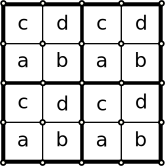
\includegraphics[scale=0.7]{quad_mesh_color_sym} \label{fig:quadCol}
	}
	\hspace{+1mm}
	\subfloat[]{
	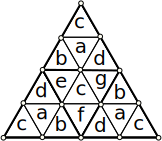
\includegraphics[scale=0.8]{triangle_mesh_color_sym} \label{fig:triaCol}
	}
	}
	\caption[Mesh element coloring]{Mesh element coloring showing two types of meshes. \protect\subref*{fig:quadCol} Structured quadrilateral mesh containing a total of four colors.  \protect\subref*{fig:triaCol}~Triangular mesh containing a total of six colors.}
	\label{fig:meshCol}
\end{figure}


\subsubsection{Partition-Parallel Message Scheduling}
Since \gls{acr:fem} elements exhibit geometrical locality in meshes, factor nodes adjacent to each other could be scheduled on the same processing element in order to compute using sequential updates; while communications between factor nodes in different processing elements can be scheduled using parallel updates.
This scheduling scheme is referred to as the \gls{acr:pps} and is illustrated in \figRef{fig:partPar}.
The nodes using the parallel schedule lie on the boundary of partitions.
As a result, the number of parallel scheduled nodes is considerably less than the number of sequentially scheduled nodes that lie in the interior of the partition.
A similar scheduling scheme was previously introduced in \chpRef{chp:PW-GaBP} and was referred to as the \gls{acr:hus} scheme \cite{bib:El-Kurdi2012EIOGBPSFLSDDLS}; however, the key distinction here is that the \gls{acr:cps} scheme can be used within each partition.

\begin{figure}
	\centering{
	\subfloat[]{
	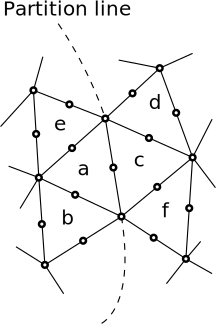
\includegraphics[scale=0.5]{partition_parallel_mesh} \label{fig:partParMesh}
	}
	\hspace{+2mm}
	\subfloat[]{
	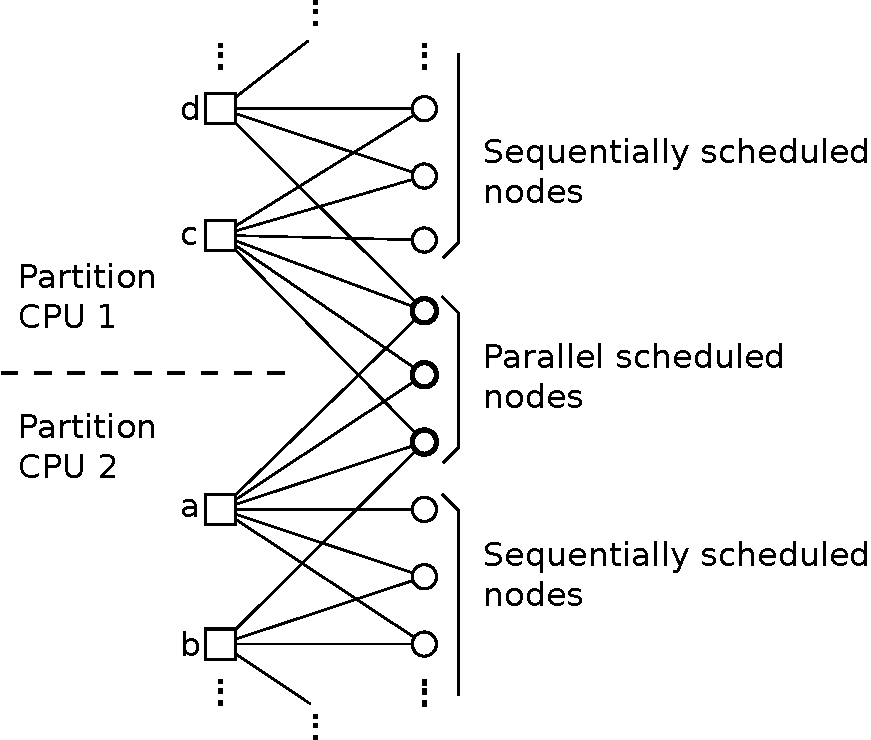
\includegraphics[scale=0.5]{partition_parallel_FG} \label{fig:partParFG}
	}
	}
	\caption[The partition-parallel Message schedule.]{The partition-parallel Message schedule. \protect\subref*{fig:partParMesh}~Hypothetical mesh. \protect\subref*{fig:partParFG}~Partitioned \gls{acr:femfg}. }
	\label{fig:partPar}
\end{figure}



\subsection{The FGaBP Algorithm Listing}
A high level listing of the \gls{acr:fgabp} algorithm is shown in \algRef{alg:FGaBP}.
The steps \ref{alg:genElmSrc} and \ref{alg:bndCnds} are considered the setup phase of the \gls{acr:fgabp} algorithm and can be performed completely in parallel.
The loop in line \ref{alg:partPar} reflects parallelism using partitions across CPUs in a cluster, which typically is programmed using \gls{acr:mpi}.
The loop in line \ref{alg:colPar} reflects parallelism using coloring across CPUs in a shared memory machine, which is programmed using multithreading.
\gls{acr:cps} implementations on shared memory machines can be performed by simply creating only one partition.
On the other hand, partition-parallel implementations can be performed by considering that each factor has its unique color; hence, the loop in line \ref{alg:colPar} is executed sequentially within a partition.
The \gls{acr:fgabp} algorithm, which encompasses a complete \gls{acr:fem} execution process, performs its computation completely in parallel without assembling or operating on any large sparse matrices.

\begin{algorithm}[h]
  %\centering
	\begin{algorithmic}[1]
		\STATE Obtain \gls{acr:fem} mesh
		\STATE Perform partition-color
		\STATE Generate element matrices $M_s$ and source vectors $B_s$ \label{alg:genElmSrc}
		\STATE Incorporate boundary conditions \label{alg:bndCnds}
		\STATE \textit{Initialize:} $\alpha_{ij} = 1,\,\, \beta_{ij} = 0,\,\,\forall i,j$
		\REPEAT[\gls{acr:fgabp} iteration: $t=1,2,\cdots$]
		\LOOP[Assign partitions to CPUs in cluster] \label{alg:partPar}
		\LOOP[For each color]
		\LOOP[Schedule factor nodes to all available CPU cores or threads] \label{alg:colPar}
		\STATE  Compute messages according to \eqnRef{eqn:vna}, \eqnRef{eqn:vnb}, \eqnRef{eqn:fnaO}, and \eqnRef{eqn:fnbO}
	\ENDLOOP
	\STATE Synchronize threads
\ENDLOOP
\STATE Synchronize parallel message buffers
\ENDLOOP
\UNTIL{Convergence check on messages}
\STATE \textit{Output:} $\mu_i = \frac{\beta_i}{\alpha_i}$
  \end{algorithmic}
  \caption{The \acrshort{acr:fgabp} algorithm.}
  \label{alg:FGaBP}
\end{algorithm}


%%%%%%%%%%%%%%%%%%%%%%%%%%%%%%%%%%%%%%%%%%%%%%%%%%%%%%%%%%%%%%%%%%%%%%%
%% Section
%%%%%%%%%%%%%%%%%%%%%%%%%%%%%%%%%%%%%%%%%%%%%%%%%%%%%%%%%%%%%%%%%%%%%%%


\section{Lower Complexity FGaBP}
\label{sec:lowerCompFGaBP}

As can be seen from the \gls{acr:fgabp} update rules in \eqnRef{eqn:vna}, \eqnRef{eqn:vnb}, \eqnRef{eqn:fnaO}, and \eqnRef{eqn:fnbO}, the \gls{acr:fgabp} computational complexity per iteration is dominated by the \gls{acr:fn} processes.
Because of the matrix inversion required by each \gls{acr:fn}, the total \gls{acr:fgabp} complexity per iteration, when using e.g. the Cholesky algorithm, is $\bigo{\gls{acr:nf} n (n-1)^3/3} \approx \bigo{\gls{acr:nf} n^4/3}$ where \gls{acr:nf} is the number of \glspl{acr:fn} in the \gls{acr:femfg} model.
For \gls{acr:fem} problems, \gls{acr:nf} is typically proportional to \gls{acr:nv}, where \gls{acr:nv} is the number of \glspl{acr:vn}.
In addition, we always have $n\ll \gls{acr:nf}$, e.g. for first order triangular meshes $n=3$ and first order tetrahedral meshes $n=4$.
More importantly, $n$ is independent of \gls{acr:nf} which implies that the \gls{acr:fgabp} algorithm can offer high parallel scalability for a good choice of message scheduling.
However, due to the high \gls{acr:fn} computational complexity, the local computational cost may dominate as $n$ increases when supporting higher degree FEM basis functions, for example when $n \geq 5$.
In the following, we present reformulations of the \gls{acr:fgabp} algorithm that considerably reduces the \gls{acr:fn} complexity to $\bigo{n^2}$.


We can reformulate the \gls{acr:fn} update rules using the partitioned matrix inversion identity as stated in the following:
\begin{equation}
	Z=\left[\begin{array}{cc}
		P & Q\\
		R & S
	\end{array}\right],\qquad Z^{-1}=\left[\begin{array}{cc}
		\tilde{P} & \tilde{Q}\\
		\tilde{R} & \tilde{S}
	\end{array}\right]
	\label{eqn:invPar}
\end{equation}
where:
\begin{align*}
	\tilde{P} & =V\\
	\tilde{Q} & =-VQS^{-1}\\
	\tilde{R} & =-S^{-1}RV\\
	\tilde{S} & =S^{-1}+S^{-1}RVQS^{-1}\\
	V & =\left(P-QS^{-1}R\right)^{-1}
\end{align*}
Comparing \eqnRef{eqn:invPar} to \eqnRef{eqn:wk} in the \gls{acr:fgabp} algorithm, we can see that $P = W^{(t_\star)}_{\mathcal{L}(i)}$, which is a single element matrix; and $R=Q^T=V$, which is a column matrix with dimensions $(n-1)\text{-by-}1$; and finally, $S = \bar{W}^{(t_\star)}$.
Then, the \gls{acr:fn} update rules can alternatively be obtained by directly computing the inverse of $W$ and partitioning it as follows:
\begin{align}
	(W^{(t_\star)})^{-1} & =\left[\begin{array}{cc}
		\tilde{W}_{\mathcal{L}(i)} & \tilde{C}^{T}\\
		\tilde{C} & \tilde{D}
	\end{array}\right] \label{eqn:fnInv}
\end{align}
The resulting \gls{acr:fn} updates will be:
\begin{align}
	\alpha_{ai}^{(t)} & =\frac{1}{\tilde{W}_{\mathcal{L}(i)}}-\alpha_{ia}^{(t_\star)} \label{eqn:fna2}\\
	\beta_{ai}^{(t)} & =B_{\mathcal{L}(i)}+\frac{1}{\tilde{W}_{\mathcal{L}(i)}}(\bar{K}^{(t_\star)})^{T}\tilde{C} \label{eqn:fnb2}
\end{align}
Using an in-place Cholesky inversion algorithm to compute $(W^{(t_\star)})^{-1}$, the \gls{acr:fn} complexity can be reduced to $\bigo{n^3/3}$.
Since $W$ is small and dense, optimized linear algebra libraries can be used to compute its inverse efficiently.
Examples of such libraries are Eigen~\cite{bib:eigen}, Gmm++~\cite{bib:gmm}, and Lapack~\cite{bib:lapack}.


For cases where $n$ is relatively large, e.g. $n\geq5$, computing the inverse can still be costly.
As shown by the \gls{acr:fem} distribution $\mathcal{P}$ in \eqnRef{eqn:statPoint}, the FEM solution requires only finding the marginal means as computed by the \gls{acr:fgabp} algorithm.
The marginal means are computed iteratively by the ratios of the nodal parameters $\beta_i$ and $\alpha_i$ as shown in \eqnRef{eqn:vnm}.
Substituting \eqnRef{eqn:vnb} into \eqnRef{eqn:fnb2} and rearranging terms we then obtain:
\begin{equation}
	\bar{u}_a^{(t)} = (W^{(t_\star)})^{-1} K^{(t_\star)} \label{eqn:locSol}
\end{equation}
which can be seen as the local element approximate solution obtained from the \fn{a} for the \vn{i} $i\in\mathcal{N}(a)$ and for fixed $\alpha$ messages.
If we partition $W$ as $W = D-E-F$ such that $D$ is the main diagonal of $W$, while $E$ and $F$ are the lower and the upper off-diagonals of $W$ correspondingly, a local stationary, fixed-point, iterative process can be created within each \gls{acr:fn}.
For example, the following will constitute a \gls{acr:gs} iteration:
\begin{equation}
	\bar{u}_a^{(t)} = (D-E)^{-1} F \bar{u}_a^{(t_\star)} + (D-E)^{-1} K^{(t_\star)}. \label{eqn:gsUpdate}
\end{equation}
Other fixed-point iterative methods such as Jacobi or \gls{acr:sor} can also be configured.


The $\alpha$ messages can be fixed after allowing the \gls{acr:fgabp} algorithm to execute normally for a couple of iterations, or until the $\alpha$ messages converge to a very high tolerance such as $10^{-1}$.
This should replace the initial values in the $\alpha$ messages with better estimates.
Then a number of iterations is executed using \eqnRef{eqn:locSol} to obtain a better estimate for $\bar{u}_a$.
In all of our experiments, one or two iterations of \gls{acr:gs} was practically sufficient.
Finally, the new $\beta_{ai}^{(t)}$ messages are obtained from the $\bar{u}_a^{(t)}$ estimates as follows:
\begin{equation}
	\beta_{ai}^{(t)} = \bar{u}_i^{(t)} \alpha_i^{(t_o)} - \beta_i^{(t_\star)} + \beta_{ai}^{(t_\star)}, \label{eqn:gsBetaUpdate}
\end{equation}
where $t_o$ is the iteration where the $\alpha$ messages are fixed.
Clearly, using this approach the \gls{acr:fn} process complexity is reduced to approximately $\bigo{n^2}$.
It can be shown that the fixed-point solutions, or marginal means, of the original \gls{acr:fgabp} update rules are equal to the fixed-point solutions of the new \gls{acr:fgabp} update rules.
However, the final message parameters, $\alpha$ and $\beta$, may be different between the two algorithms.
We refer to this reduced complexity algorithm as the \gls{acr:aufgabp} algorithm.
\tableRef{tbl:FGaBPUpdRules} summarizes the equations for the \gls{acr:fgabp} \gls{acr:fn} update rules and the associated computational complexity for a relatively large $n$.

\begin{table}
	\centering
	\begin{threeparttable}
		\caption{Summary of the \acrshort{acr:fgabp} update rules.} \label{tbl:FGaBPUpdRules}
		\begin{tabular}{lll} 
			\toprule
			Algorithm            & \gls{acr:fn} Update Equations                                                           & \gls{acr:fn} Complexity \tabularnewline
			\midrule
			Exact updates        & \eqnRef{eqn:fnaO}, \eqnRef{eqn:fnbO}                                                    & $O(n^4)$ \tabularnewline
			Exact updates        & \eqnRef{eqn:fna2}, \eqnRef{eqn:fnb2}                                                    & $O(n^3)$ \tabularnewline
			Approximated updates & \eqnRef{eqn:locSol}\tnote{1}, \eqnRef{eqn:gsUpdate}\tnote{2}, \eqnRef{eqn:gsBetaUpdate} & $O(n^2)$ \tabularnewline
			\bottomrule
		\end{tabular}
		\begin{tablenotes}
			\begin{footnotesize}
			\item[1] {Fixed $\alpha$ messages.}
			\item[2] {Using the \gls{acr:gs} iteration.}
			\end{footnotesize}
		\end{tablenotes}
	\end{threeparttable}
\end{table}


\section{Element Merging}
\label{sec:elmMerg}


In this section, variations on the graphical structure of the \gls{acr:fgabp} algorithm are proposed in order to increasing the parallel efficiency of the \gls{acr:fgabp} execution on multicore architectures with suitable cache capacities.
By virtue of the factorization structure of the \gls{acr:femfg} model, we can easily redefine new factors in \eqnRef{eqn:fgpf} by joining other factors as follows:
\begin{equation}
	\Psi_{\hat{s}}(U_{\hat{s}}) = \Psi_{s_1}(U_{s_1}) \Psi_{s_2}(U_{s_2}),
	\label{eqn:jpdf}
\end{equation}
where factors $s_1$ and $s_2$ are joint into factor $\hat{s}$, which is a function of the variable set $U_{\hat{s}} = U_{s_1} \cup U_{s_2}$.
Once suitable elements are identified for merging, the \gls{acr:fgabp} algorithm can be executed normally after locally assembling the merged elements' matrices and source vectors, $M_{\hat{s}}$ and $B_{\hat{s}}$ correspondingly.
When the factors are adjacent, the cardinality of $U_{\hat{s}}$ is $\cardinal{U_{\hat{s}}} = \cardinal{U_{s_1}} + \cardinal{U_{s_2}} - \cardinal{U_{s_1} \cap U_{s_2}}$.
If $U_{s_1}$ and $U_{s_2}$ are not adjacent, or disjoint, then $U_{s_1} \cap U_{s_2} = \emptyset$.
\Gls{acr:em} can be particularly advantageous if elements that share edges in 2D meshes or surfaces in 3D meshes are merged.
As a result, the memory bandwidth utilization can improve due to the considerable reduction in the total number of edges in the FEM-FG model. 
By merging adjacent elements, we can better utilize the high CPU computational throughput in exchange for the slower memory bandwidth and latency.


EM can be mainly useful for 2-D triangular and 3-D tetrahedral meshes with first order \gls{acr:fem} elements.
To quantify the effect of merging, we define the \gls{acr:mrr} percentage by dividing the amount of reduced memory from the merge by the original amount of memory before the merge.
The MRR is computed as:
\begin{equation}
	\OpN{MRR} = \frac{\sum_{a \in \mathcal{D}}M_a - \sum_{a \in \mathcal{C}}M_a}{\sum_{a \in \mathcal{D}}M_a} \cdot 100\%,
\end{equation}
where $\mathcal{D}$ is the set of all factors before any merge, $\mathcal{C}$ is the set of merged factors, and $M_a$ is the amount of memory required for \fn{a}.
As later shown in \secRef{sec:fgabpImp}, the memory complexity per \gls{acr:fn} can be obtained by $M_i \propto \bigo{4n_a+n_a^2}$ where $n_a$ is the number of \fn{a} edges, or the rank of $M_a$.
If we consider structured meshes for illustration purposes only, the resulting \gls{acr:mrr} is 23.8\% when merging every two adjacent triangles into a quadrilateral, or 46.4\% when merging every four fully connected triangles into a quadrilateral.
\figRef{fig:elm_merge} illustrates the different \gls{acr:femfg} graphs resulting from merging every two or every four adjacent triangles in a structured triangular mesh.


For irregular triangular meshes with large numbers of triangles, the Euler's formula \cite[p.~28]{bib:Berg2008CGA} states that each vertex will be surrounded by six triangles on average.
Thus, when merging mostly six triangle groups into hexagons, the \gls{acr:mrr} increases, on a per merge basis, to 38.9\%, or to 42.9\% when merging five triangles.
Merging triangles does not have to be uniform.
We may decide to merge patches of 2, 3, 4, 5, 6, or more as long as the triangles share edges and form connected or, preferably, convex regions.
Similarly for 3D tetrahedral meshes, merging tetrahedrons sharing faces can also result in significant memory storage reductions.
If two tetrahedrons of first order are merged, the \gls{acr:mrr} is 29.7\%, and 53.1\% when merging three tetrahedrons sharing faces and are enclosed by five vertices.


\def \MyVariableScale{.7}
\def \MyVariableSeparation{1cm}
\begin{figure}[h]
	\centering
	{
	\subfloat[]{%
	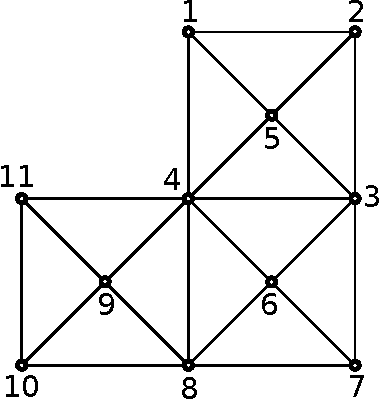
\includegraphics[scale=\MyVariableScale]{fg_triangle_merge_a} \label{fig:elm_merge_a}
	}
  %\hfil
	\hspace{\MyVariableSeparation}
	\subfloat[]{%
	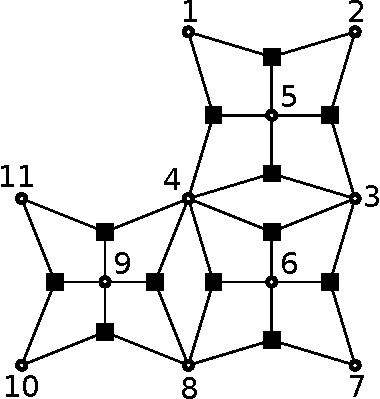
\includegraphics[scale=\MyVariableScale]{fg_triangle_merge_b} \label{fig:elm_merge_b}
	}
	\vfill
	\subfloat[]{%
	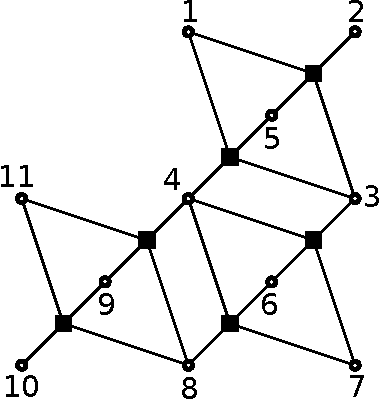
\includegraphics[scale=\MyVariableScale]{fg_triangle_merge_c} \label{fig:elm_merge_c}
	}
  %\hfil
	\hspace{\MyVariableSeparation}
	\subfloat[]{%
	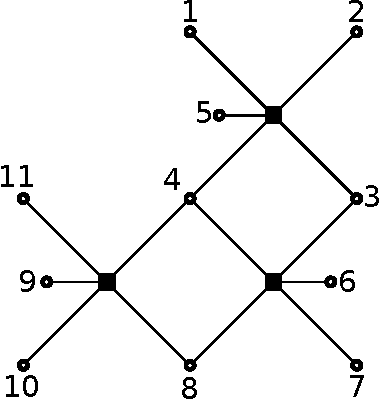
\includegraphics[scale=\MyVariableScale]{fg_triangle_merge_d} \label{fig:elm_merge_d}
	}
	}
	\caption[Element merging examples.]{Triangular element merging examples. \protect\subref*{fig:elm_merge_a}~Original triangular mesh. \protect\subref*{fig:elm_merge_b}~The initial \gls{acr:femfg} using single element factorization. \protect\subref*{fig:elm_merge_c}~Merging two adjacent triangles. \protect\subref*{fig:elm_merge_d}~Merging adjacent four triangles.}
	\label{fig:elm_merge}
\end{figure}


While merging elements based on a structured mesh is a trivial operation, we can still efficiently merge certain element configurations in unstructured meshes with the aid of partitioning algorithms \cite{bib:parmetis2013,bib:parmetisMan,bib:metis,bib:parmetisKarypis1996}.
For such cases, the partitioning algorithms can be used to isolate the desired patches of elements.
Specifically, the work in \cite{bib:ChanAgg} presents algorithms to create macro-elements by joining adjacent elements in unstructured grids.
Partitioning may add some overhead in the preprocessing stage; however, since in practice the number of factors is much greater than the number of CPU cores, a lower partition quality can be used to lower the partitioning overhead time \cite{bib:parmetisMan} without having much impact on the overall parallel efficiency.

The element merging does not affect the underlying FEM mesh discretization properties, it does however affect the \gls{acr:fgabp} numerical complexity as a solver.
Our results in \secRef{sec:elmMergRes} reveal that the overall computational complexity of the merged \gls{acr:femfg} can be higher than that of the original, un-merged one.
Nonetheless, the \gls{acr:fgabp} demonstrates considerable speedups for the merged \gls{acr:femfg} structure, because of better utilization of available memory bandwidth and cache resources resulting from an improved computational locality.
These observations are illustrated in \secRef{sec:elmMergRes}.
To conclude, we propose to use the merge feature as a high-level means to control trade-offs between CPU resources such as memory bandwidth, cache utilization, and CPU cycles to facilitate fine-tuned implementations on manycore architecture.


\section{Implementation}
\label{sec:fgabpImp}

\subsection{Data-structures}
\label{sec:fgabpDS}

Using the \gls{acr:cps} scheme of \gls{acr:fgabp} and assuming all \glspl{acr:fn} are of the same size, the overall storage requirement of \gls{acr:fgabp} is $\bigo{2 \gls{acr:nv}+\gls{acr:nf}(n^2+4n)}$ in 64-bit words.
This includes two vectors of size \gls{acr:nv} for the \gls{acr:vn}'s $\alpha_i$ and $\beta_i$, and a data-structure of size \gls{acr:nf} containing the \glspl{acr:fn} data-structures where each \gls{acr:fn}'s data-structure contains a dense matrix $M_a$, vectors $B_a$, $\alpha_{ai}$, and $\beta_{ai}$, and a 64-bit integer vector storing local to global index associations.
This setup, also, assumes that all indices are stored in 64-bit integers and all real numbers are stored in 64-bit \gls{acr:dpfp}, which is essential for very large problems.
Since usually $\bigo{\gls{acr:nf}}\approx \bigo{\gls{acr:nv}}$, the overall \gls{acr:fgabp} memory complexity is $\bigo{\gls{acr:nv}}$, typical for sparse problems.
However, unlike conventional sparse data-structures such as the \gls{acr:csr}, all the \gls{acr:fgabp} data is contiguous, or dense.
Hence, the \gls{acr:fgabp} data-structure adds minimal overhead by eliminating the need to store complicated sparsity patterns.
For certain cases where the problem size does not require 64-bit indices, e.g. when approximately $10^6<\gls{acr:nv}<10^8$, 32-bit indices can be used instead.
For such a case, the \gls{acr:fgabp} memory complexity will be slightly lower to $\bigo{2 \gls{acr:nv}+\gls{acr:nf}(n^3+2.5n)}$.


In order to compare the \gls{acr:fgabp} data-structure with the other sparse data-structures in terms of storage size, we use the \gls{acr:srm} as follows:
\begin{align}
	\OpN{\acrshort{acr:srm}} & = \frac{\text{Other sparse storage}}{\text{\gls{acr:fgabp} storage}}\\
	& = \frac{2 \gls{acr:nnz} +2 \gls{acr:nv}}{2 \gls{acr:nv}+\gls{acr:nf}(n^3+4n)}. \label{eqn:srmCSR}
\end{align}
In \eqnRef{eqn:srmCSR} we are considering the \gls{acr:csr} storage size as an example for comparison due to its popularity.
As shown in \figRef{fig:csr}, the size of the \gls{acr:csr} format includes a vector of size \gls{acr:nv} for the row start index, and two vectors of size \gls{acr:nnz} for the element value and its row index. 
In addition, the right-hand-side vector of size \gls{acr:nv} is added to the \gls{acr:csr} format, in order to provide a consistent comparison with the \gls{acr:fgabp} format which already includes the elements' source vectors in its storage.
It is important to note that in practice the sparse storage for other solvers is typically much larger than what is used here in the \gls{acr:srm}; since, iterative solvers such as the \gls{acr:pcg}, as in \algRef{alg:pcg}, would required additional memory to store the preconditioner as well as the search and residual vectors.
On the other hand, the \gls{acr:fgabp} data-structure includes all the information needed to solve the \gls{acr:fem} problem rather than just storing the sparse matrix of the global linear system.
However, since implementations of the \gls{acr:pcg} algorithm may vary from one library to another, we will not consider its full storage in the \gls{acr:srm} analysis, but rather only the storage required for the sparse matrix and the right-hand-side vector.

\subsection{The FEM-FG Edges}

Another metric we use in our analysis is the \gls{acr:lrm} defined as follows:
\begin{align}
	\OpN{\acrshort{acr:lrm}} & = \frac{\text{Number of edges in the \gls{acr:pwgm}}}{\text{Number of edges in the \gls{acr:femfg} model}}\\
	& = \frac{(\gls{acr:nnz}-\gls{acr:nv})/2}{\gls{acr:nf} n}.
\end{align}
The \gls{acr:lrm} is a measure for the amount of information the algorithm is required to communicate per iteration.
As we will see later in \secRef{sec:fgabpRes}, this ratio may explain some of the convergence behavior of \gls{acr:fgabp} in comparison to other sparse algorithms.
It is important to note that the \gls{acr:lrm} is not a measure for the memory bandwidth requirement of a particular algorithm.
The \gls{acr:srm} may be a closer measure to the memory bandwidth required by the solver per iteration.
However, the memory bandwidth is not easy to measure because, not only does it depends on the amount of data needed to be accessed, but rather it depends more on the access pattern of the sparse data-structure.
That is because at the hardware level, the memory controllers respond to the CPU's memory requests by sending data in contiguous chunks, as in memory lines, which is stored temporarily in the cache memory \cite{bib:Hennessy2012CAQA}. 
The CPU on the other hand, uses the cache memory to retrieve exactly what it needs.
This is the key reason behind the notoriously poor performance of sparse data-structures.
If the data is not contiguous in memory, then the CPU only utilizes a small fraction of the data transfer to the cache.
This leads to under-utilized cache or poorly utilized memory bandwidth causing an overall poor computational throughput.
The \gls{acr:fgabp}, on the other hand, utilizes contiguous data-structures which considerably improves its memory bandwidth utilization.

\tableRef{tbl:FEMFGAnal} illustrates the \gls{acr:srm} and the \gls{acr:lrm} trends for a number of meshes.
The L-shaped domain is used as the example domain.
The open-source software \libName{Gmsh} \cite{bib:gmsh2009} is used to mesh the domain.
The triangular, tetrahedral and quadrilateral meshes are unstructured, while the hexahedral meshes are structured and also generated by \libName{Gmsh}.
The stiffness matrix was obtained for the Laplace equation using the software package \libName{GetFEM} \cite{bib:getfem}.
Using the stiffness matrix, we can obtain the number of edges for the corresponding \gls{acr:pwgm} using the actual \gls{acr:nnz} of the matrix.
Clearly, for both ratio metrics the \gls{acr:fgabp} shows a progressively increasing advantage as the \gls{acr:fem} order increases for all types of meshes.
In particular, the \gls{acr:lrm} shows considerable advantage for all types of meshes except the first order triangular and tetrahedral meshes.
However, this can be efficiently remedied using the \gls{acr:em} feature discussed earlier in \secRef{sec:elmMerg}.

%%%%%%%%%%%%%%%%%%%
%% This table is rotated in landscape mode
%%%%%%%%%%%%%%%%%%
\afterpage{%
\clearpage% Flush earlier floats (otherwise order might not be correct)
%\thispagestyle{empty}% empty page style (?)
\begin{sidewaystable}% Landscape page
	%\begin{table}[t]
	\centering
	\begin{threeparttable}[t]
		\caption{The \acrshort{acr:femfg} comparison analysis.} \label{tbl:FEMFGAnal}
		\begin{tabular}{lrrrrrrrr>{\itshape}r>{\itshape}r} 
			\toprule
			\multicolumn{1}{c}{Element}& \multicolumn{1}{c}{$n$ \tnote{1}}& \multicolumn{1}{c}{\gls{acr:nv}}& \multicolumn{1}{c}{\gls{acr:nf}}& \multicolumn{1}{c}{\gls{acr:nnz}}& \multicolumn{1}{c}{\acrshort{acr:pwgm}}& \multicolumn{1}{c}{Sparse}& \multicolumn{1}{c}{\acrshort{acr:femfg}}& \multicolumn{1}{c}{\acrshort{acr:femfg}}& \multicolumn{1}{c}{\acrshort{acr:srm}}& \multicolumn{1}{c}{\acrshort{acr:lrm}} \tabularnewline
			\multicolumn{1}{c}{Geometry}& & &  &  & \multicolumn{1}{c}{Edges}& \multicolumn{1}{c}{Storage\tnote{2}}& \multicolumn{1}{c}{Edges}& \multicolumn{1}{c}{Storage \tnote{3}}&  & \tabularnewline
			\midrule
			triangle      & 3  & 349   & 634  & 2313    & 982     & 6372    & 1902   & 14012   & 0.45 & 0.52 \tabularnewline
			triangle      & 6  & 1331  & 634  & 14831   & 6750    & 36318   & 3804   & 40702   & 0.89 & 1.77 \tabularnewline
			triangle      & 10 & 2947  & 634  & 48967   & 23010   & 112670  & 6340   & 94654   & 1.19 & 3.63 \tabularnewline
			triangle      & 15 & 5197  & 634  & 119937  & 57370   & 265860  & 9510   & 191084  & 1.39 & 6.03 \tabularnewline
			triangle      & 3  & 1092  & 2070 & 7414    & 3161    & 20289   & 6210   & 45654   & 0.44 & 0.51 \tabularnewline
			triangle      & 6  & 4253  & 2070 & 48059   & 21903   & 117384  & 12420  & 132706  & 0.88 & 1.76 \tabularnewline
			triangle      & 10 & 9484  & 2070 & 159196  & 74856   & 365813  & 20700  & 308768  & 1.18 & 3.62 \tabularnewline
			triangle      & 15 & 16785 & 2070 & 390505  & 186860  & 864936  & 31050  & 623520  & 1.39 & 6.02 \tabularnewline
			quadrilateral & 4  & 1057  & 1000 & 9169    & 4056    & 23624   & 4000   & 34114   & 0.69 & 1.01 \tabularnewline
			quadrilateral & 9  & 4113  & 1000 & 64449   & 30168   & 149464  & 9000   & 125226  & 1.19 & 3.35 \tabularnewline
			quadrilateral & 16 & 9169  & 1000 & 225841  & 108336  & 497528  & 16000  & 338338  & 1.47 & 6.77 \tabularnewline
			tetrahedron   & 4  & 689   & 2668 & 8343    & 3827    & 20132   & 10672  & 86754   & 0.23 & 0.36 \tabularnewline
			tetrahedron   & 10 & 4521  & 2668 & 112989  & 54234   & 248584  & 26680  & 382562  & 0.65 & 2.03 \tabularnewline
			tetrahedron   & 20 & 14165 & 2668 & 619257  & 302546  & 1309340 & 53360  & 1308970 & 1.00 & 5.67 \tabularnewline
			hexahedron    & 8  & 2448  & 1815 & 54400   & 25976   & 121041  & 14520  & 179136  & 0.68 & 1.79 \tabularnewline
			hexahedron    & 27 & 16951 & 1815 & 966985  & 475017  & 2018726 & 49005  & 1553057 & 1.30 & 9.69 \tabularnewline
			hexahedron    & 8  & 4896  & 3993 & 115574  & 55339   & 255629  & 31944  & 393120  & 0.65 & 1.73 \tabularnewline
			hexahedron    & 27 & 35443 & 3993 & 2099065 & 1031811 & 4375346 & 107811 & 3413027 & 1.28 & 9.57 \tabularnewline
			\bottomrule
		\end{tabular}
		\begin{tablenotes}
			\begin{footnotesize}
			\item[1] {$n$ is the number of variables per element.}
			\item[2] {Using \gls{acr:csr} format.}
			\item[3] {All storage estimates are in the order of \gls{acr:dpfp} numbers.}
			\end{footnotesize}
		\end{tablenotes}
	\end{threeparttable}
	%\end{table}
\end{sidewaystable}
\clearpage% Flush page
}

For certain cases, the \gls{acr:lrm} data can be analytically explained.
Considering the Euler theorem \cite[p.~28]{bib:Berg2008CGA} for triangular meshes of the first order, the ratio of edges to elements is $3/2$, now dividing by the number of factor variables (which is $n=3$ for triangular factors), then the resulting ratio should be $0.5$ as predicted by the tabulated results for first order triangles.
If we consider approximating the unstructured quadrilateral mesh with a regular one, with uniform gird points, and noting that for an isolated quadrilateral element there are six \gls{acr:fem} edge couplings, then the ratio of edges to elements approaches 4 which explains the 1.01 ratio.
Similarly for hexahedral meshes on cubical domains of dimension $N$, the number of edges for $N^3$ hexahedrons approaches $14N^3 + \bigo{N^2}$ leading to a ratio of $14/8$ which explains the 1.79 and 1.73 ratios.


\subsection{CPU Multicore Implementation}

The \gls{acr:fgabp} code was designed using C++ \gls{acr:oop} \cite{bib:c++stroustrup2013,bib:c++prata2004}.
The \gls{acr:oop} based design of the \gls{acr:fgabp} software facilitates its integration with existing frameworks of open-source libraries such as \dealName{} \cite{bib:dealii2007} and \libName{GetFEM++} \cite{bib:getfem}.
The following section presents the numerical results on the performance of both the basic \gls{acr:fgabp} and the modified \gls{acr:aufgabp} algorithms.
We utilize meshes and \gls{acr:fem} setup generated from three open-source libraries, which are \libName{Gmsh}, \libName{GetFEM++}, and \dealName{}.
We validate the \gls{acr:fgabp} algorithms on both regular and irregular meshes using various \gls{acr:fem} interpolation orders and geometrical elements shapes such as triangles, quadrilaterals, and hexahedrons.
We utilize 2D and 3D domains with various boundary conditions.


For CPU multicore implementations, the \libName{OpenMP} \cite{bib:openmp} standard \gls{acr:api} is used to parallelize the \gls{acr:fgabp} code.
Using the \gls{acr:cps} scheme, the color loops are parallelized such that each thread executes a \gls{acr:fn} routine.
Thread synchronization directives are used only at the execution end of each color group; that is, the number of synchronization directives is equal to the number of color groups in the \gls{acr:cps} scheme.


\section{The FGaBP Numerical Results and Discussions}
\label{sec:fgabpRes}

\subsection{FGaBP Verification}
\label{sec:fgabpVer}

In this section, we verify the numerical results of the new \gls{acr:aufgabp} formulation using the definite Helmoltz problem with known solution as provided by the \dealName{} library for 2D and 3D domains as well as higher order \gls{acr:fem} elements.
The definite Helmholtz is formulated as follows:
\begin{align}
	-\nabla\cdot\nabla u+ u &= g, \text{ on } \Omega \label{eqn:Helm}\\
	u &= f_1, \text{ on } \partial D \label{eqn:HelmD}\\
	\textbf{n}\cdot \nabla u &= f_2, \text{ on } \partial N \label{eqn:HelmN}
\end{align}
where $\partial D$ and $\partial N$ are the Dirichlet and Neumann boundaries such that $\partial D \cup \partial N = \partial \Omega$, and $\Omega$ is the square or cubic domain bounded by $[-1,1]$.
Equation \eqnRef{eqn:HelmN} constitutes the non-homogeneous Neumann boundary condition.
The right-hand-side functions are set, such that the exact solution is:
\begin{equation}
	u(p) = \sum_i^3 \exp\left( - \frac{| p - p_i |^2}{\sigma^2} \right)
	\label{eqn:exactSol}
\end{equation}
where $p$ is a spatial variable in $(x,y,z)$, $p_i$ are exponential center points chosen arbitrarily, and $\sigma = 0.125$.
The library \dealName{} creates the mesh, and provides the \gls{acr:fgabp} class with the elements' $M_s$, $B_s$ matrices, as well as, the local to global index data.
The \gls{acr:fgabp} processes the \gls{acr:fem} problem element-by-element in parallel and sends the end solution back to \dealName{} which computes the final error relative to the exact solution.



The \gls{acr:aufgabp} uses $\alpha$ message tolerance of $10^{-1}$ and two GS iterations.
The test cases are obtained by varying the \gls{acr:fem} element order from the 1\ssst to the 3\ssrd order for both 2D quadrilaterals and 3D hexahedrals.
\figRef{fig:HelmRes} shows the error plots for each test case.
The global error for each test case is obtained by summing the squares of the $l^2$-norm error of each element and then taking the square root of that value.
It can be seen that the \gls{acr:aufgabp} obtains the expected error trends for the \gls{acr:fem} showing increased accuracy on all test cases for both trends of increasing number of elements as well as increasing \gls{acr:fem} order.

\begin{figure}[t]
	\centering{
	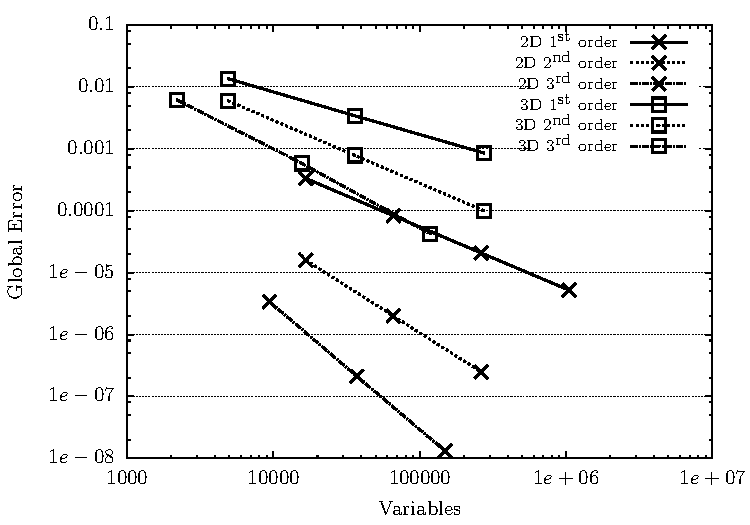
\includegraphics[scale=1.3]{plot_Helm_2D3D.pdf}
	}
	\caption[The global error performance of the AU-FGaBP.]{The global error of the AU-FGaBP obtained from element-based $l^2$-norm error relative to the exact solution.}
	\label{fig:HelmRes}
\end{figure}


\subsection{Performance Comparison}

The \gls{acr:fgabp} algorithm performance is demonstrated by solving Poisson's equation on a \gls{acr:ssc} with two dielectric media as shown in \figRef{fig:msf}.
The domain includes Dirichlet and homogeneous Neumann boundary conditions and is meshed with an irregular triangular mesh.
Different trials are performed by increasing the order of the \gls{acr:fem} interpolation from the 1\ssst order to the 5\ssth order while reducing the number of elements so as to keep the number of unknowns approximately similar.
As can be seen from the \gls{acr:lrm} data, the \gls{acr:femfg} model reduces memory communication for element orders greater than one by reducing the number of nodal links in the resulting \gls{acr:femfg} model compared to solvers such as the \gls{acr:pwgabp}.
With respect to algebraic solvers such as the \gls{acr:cg}, the link number directly correlates with the required memory communication.

\begin{figure}[t]
	\centering
	{
  %\hspace{-1mm}
	\subfloat[]{%
	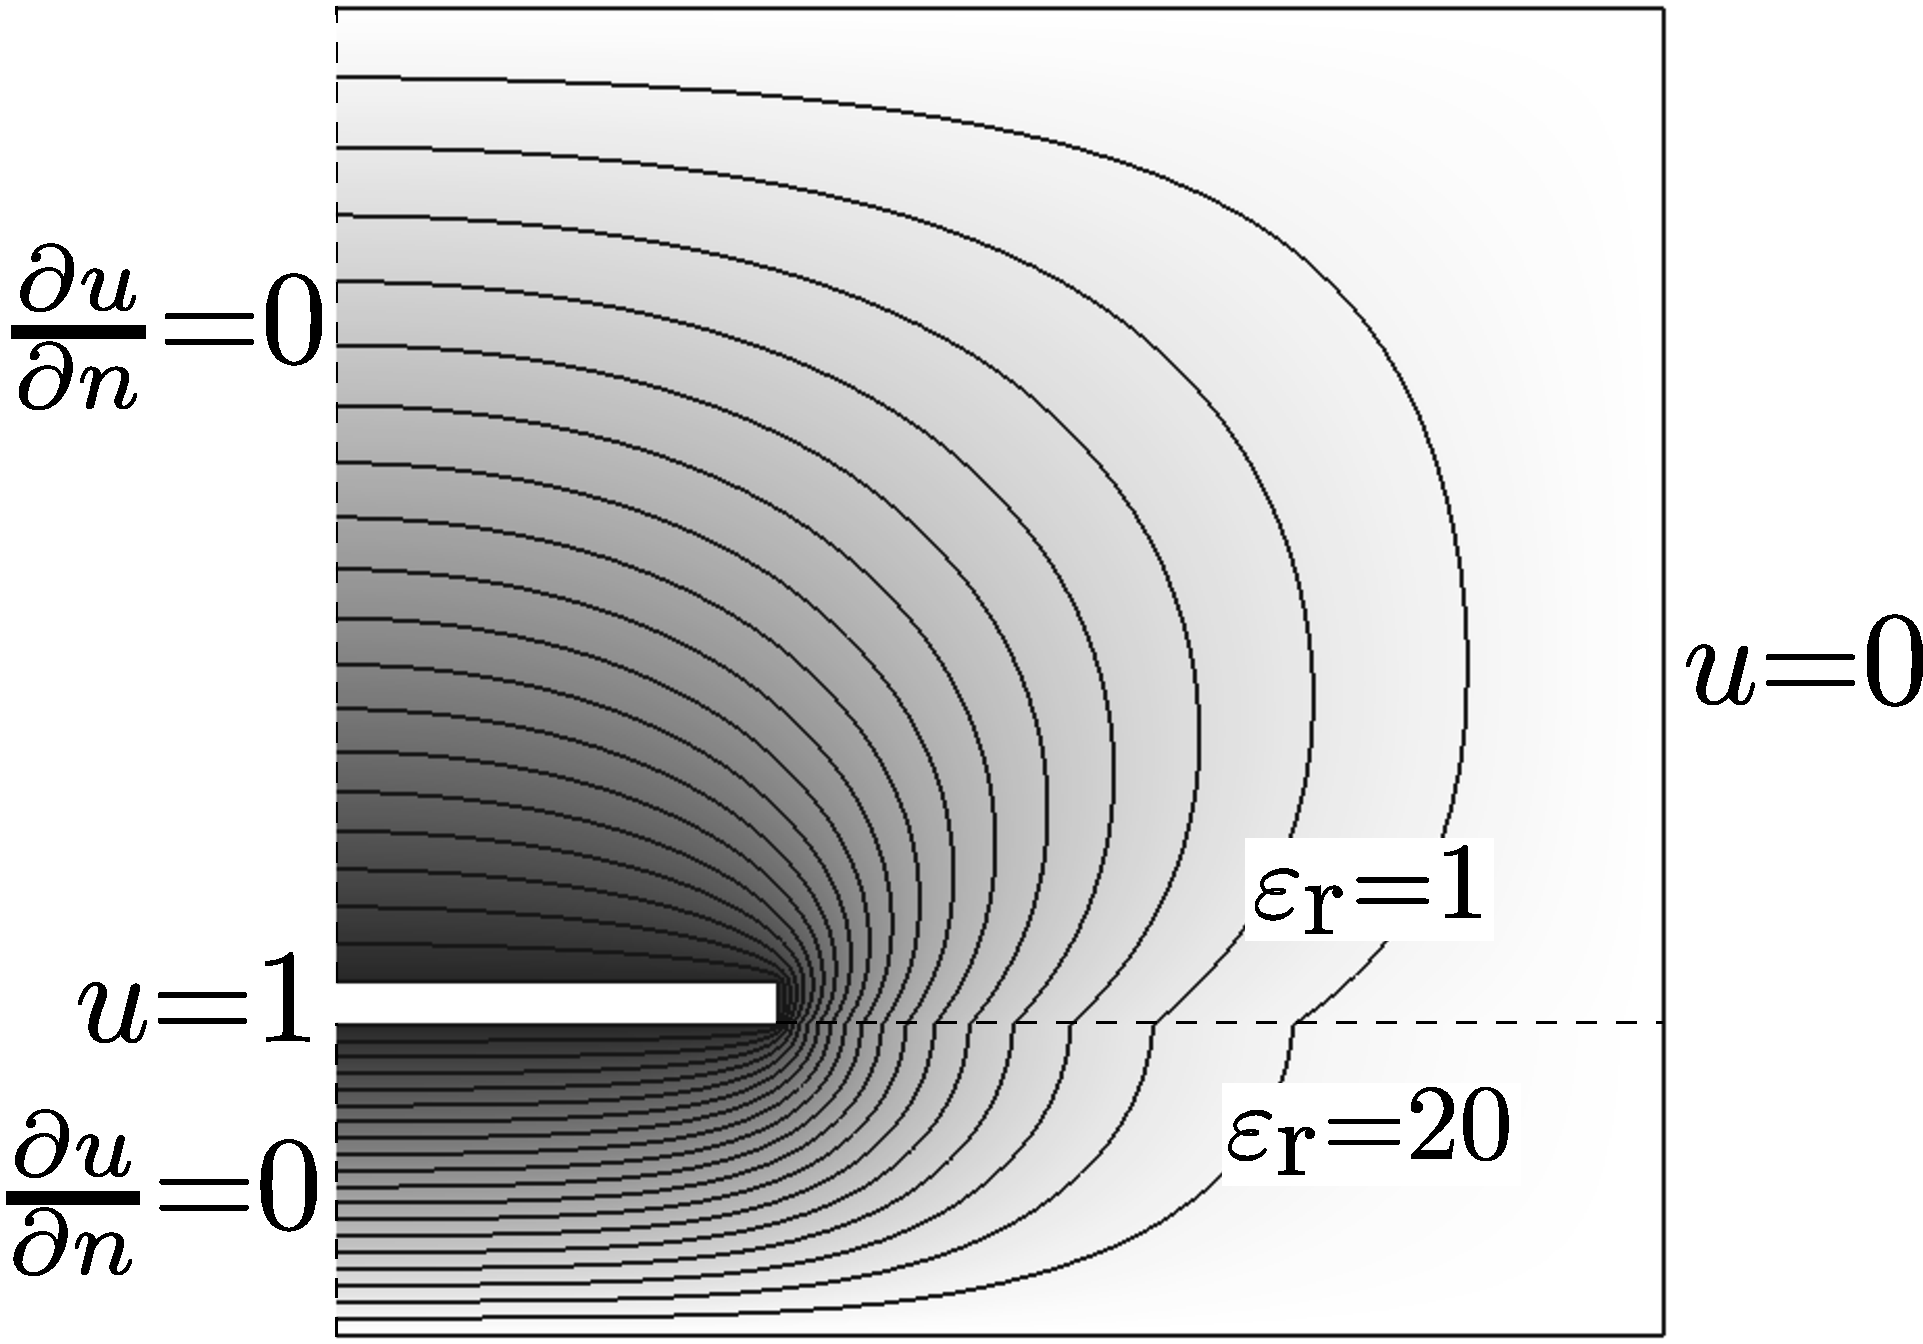
\includegraphics[scale=0.2]{FIG8}
	\label{fig:msf}
	}
	\hspace{+4mm}
	\subfloat[]{%
	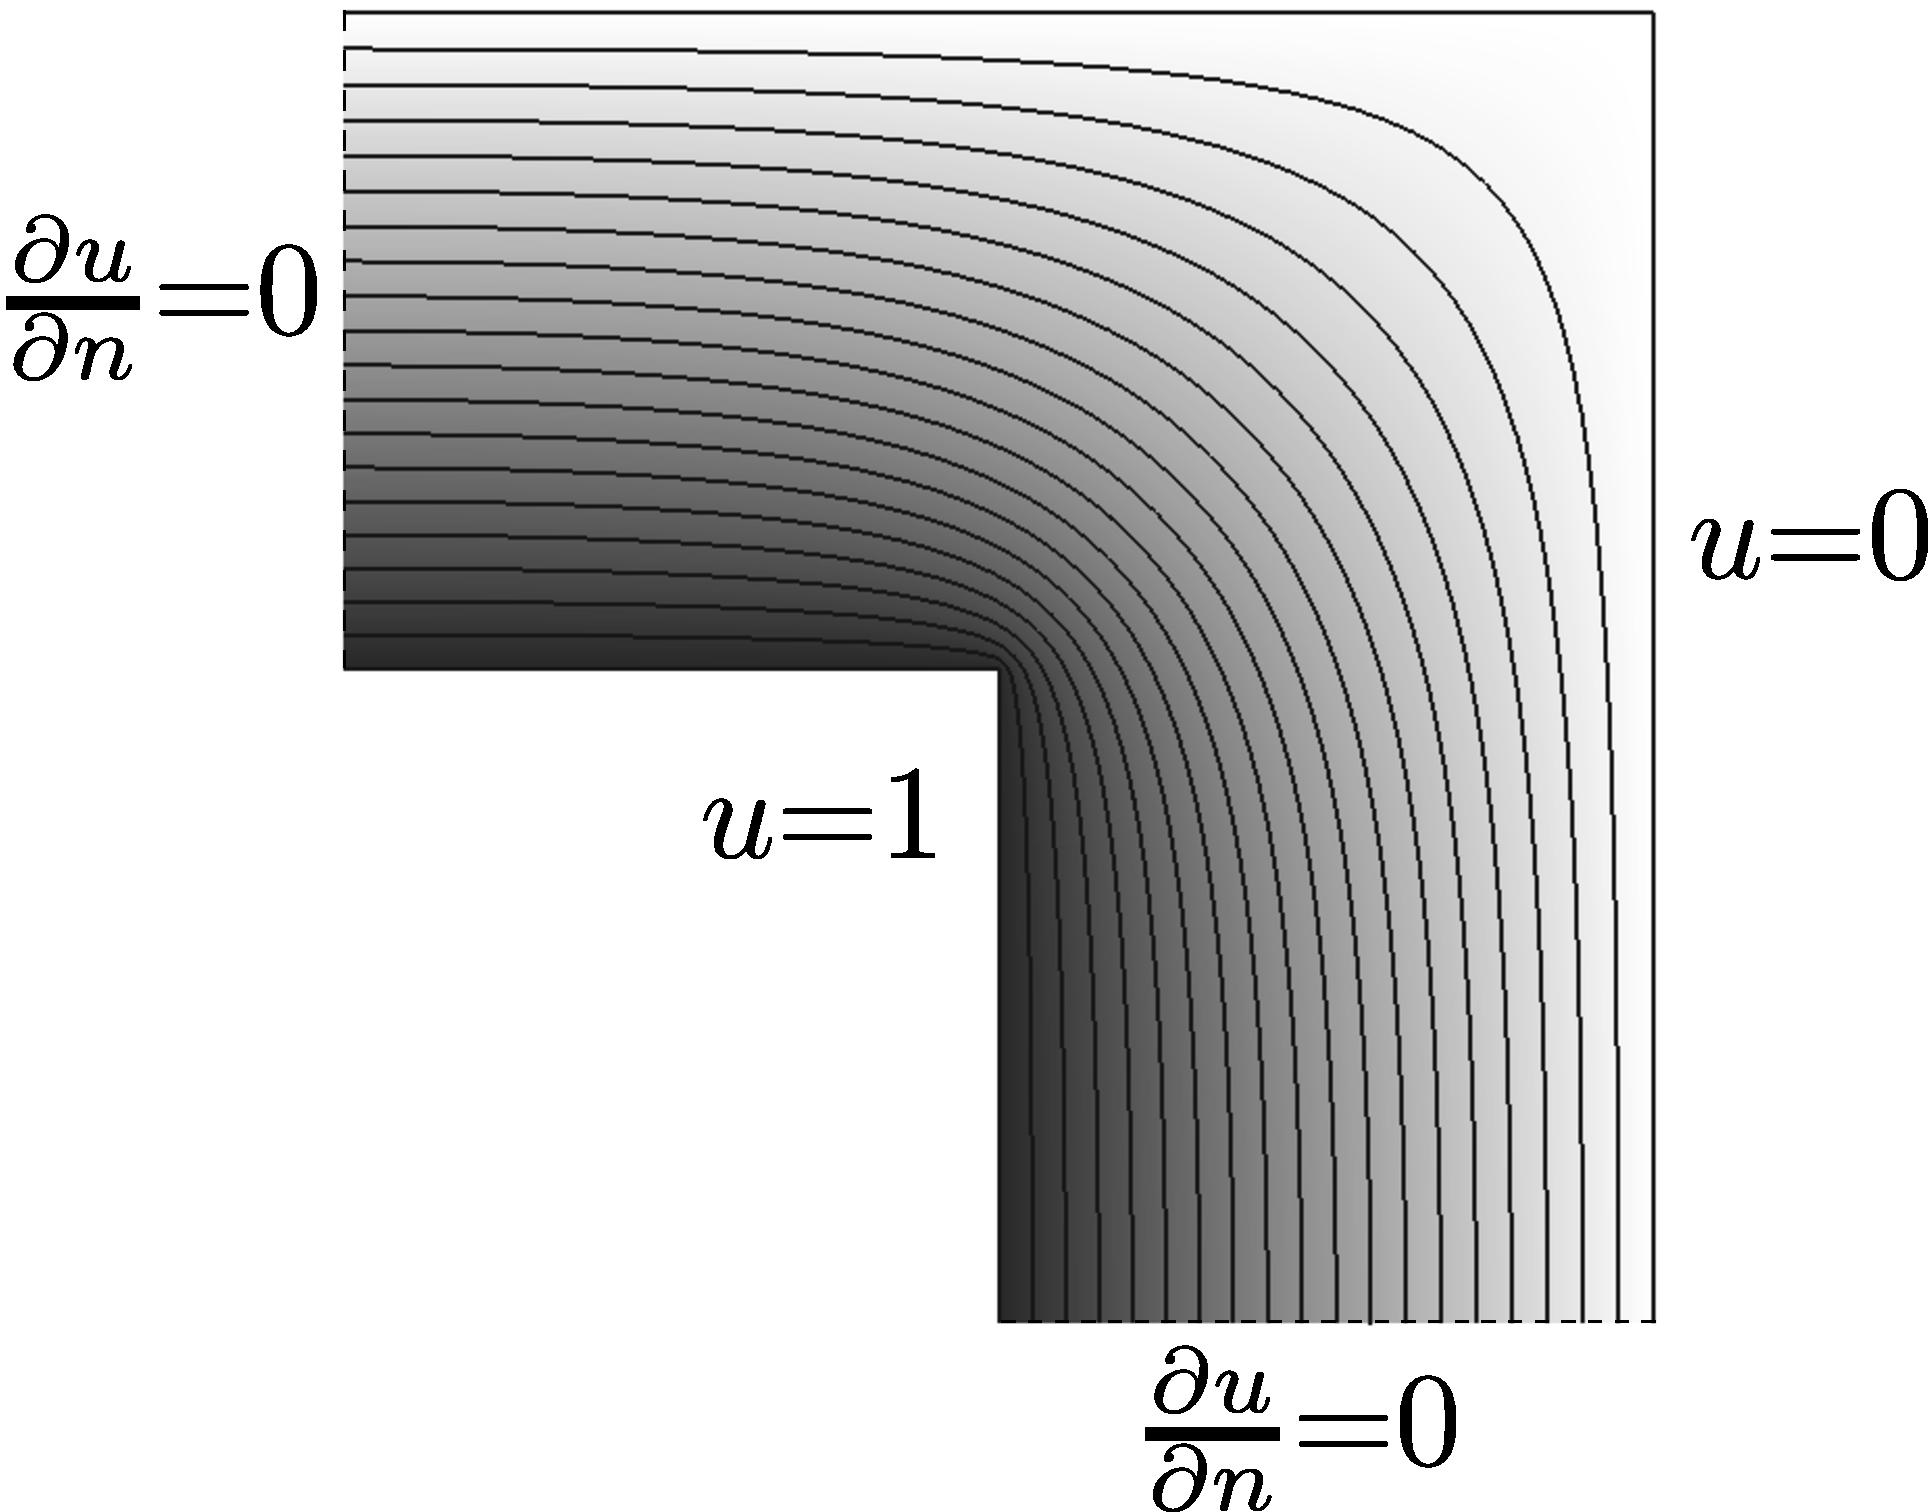
\includegraphics[scale=0.18]{FIG9}
	\label{fig:lsf}
	}
	}
	\caption[The Laplace equipotential contour lines.]{The Laplace equipotential contours obtained using \gls{acr:fgabp}, the dimensions of both structures are within the unit interval $\left[ 0,1 \right]$ cm. \protect\subref*{fig:msf} The right symmetrical side of the shielded strip between two different materials. \protect\subref*{fig:lsf} The top-right symmetrical corner of the square coaxial conductor.}
	\label{fig:ps}
\end{figure}


Also shown in \tableRef{tbl:FGaBPRes} are the iteration results of the \gls{acr:fgabp}, the \gls{acr:pwgabp}, and the \gls{acr:dpcg}.
The iterations were terminated on all experiments when the $l^2$-norm was dropped to $10^{-9}$.
We used our automatic relaxation scheme, previously introduced in \chpRef{chp:relGaBP}, to accelerate the convergence of both the \gls{acr:pwgabp} and the \gls{acr:fgabp}.
The \gls{acr:pwgabp} used \gls{acr:nmr}; whereas, the \gls{acr:fgabp} used \gls{acr:emr}.
It is important to note that the \gls{acr:pwgabp} and the \gls{acr:dpcg} require global large sparse matrix operations in each iteration which limit their effectiveness for parallel implementations; while in contrast, the \gls{acr:fgabp} requires completely decoupled computations performed element-by-element.
The last column of \tableRef{tbl:FGaBPRes} shows the \gls{acr:su} results of \gls{acr:fgabp} using a \gls{acr:cps} implementation on a quad-core CPU over the sequential one on the same workstation.
Although the implementation was not optimized to take advantage of specialized CPU features, the \gls{acr:fgabp} illustrated increased efficiency of parallel implementation as the interpolation order increases.
This is due to the \gls{acr:fgabp} making good use of increased localized computations and reduced memory communications which is a direct result from the \gls{acr:femfg} graph that reduces nodal links.


While the \gls{acr:dpcg} algorithm demonstrated the lowest iteration count, the \gls{acr:fgabp} algorithm demonstrated a trend of reducing number of iterations as the \gls{acr:fem} order increases; which illustrates its increased computational stability.
This is mainly due to the \gls{acr:fgabp} algorithm performing localized computations on small dense matrices up to order 5 instead of operating on very large sparse matrices that become increasingly ill-conditioned as the order of the \gls{acr:fem} interpolation increases.
This is a key advantage in comparison to algebraic based solvers such as the \gls{acr:pcg} whose iteration count increases as the condition number of the global characteristic matrix increases due to increasing \gls{acr:fem} order.


Even though at this stage, the \gls{acr:fgabp} algorithm does not seem to be competitive enough with the \gls{acr:pcg} solver iteration-wise, this problem will be remedied by introducing a multigrid scheme for the \gls{acr:fgabp} algorithm as will be shown later in \chpRef{chp:FMGaBP}. 
Lastly, as can also be seen in \tableRef{tbl:FGaBPRes}, the \gls{acr:pwgabp} failed to converge as the interpolation order increased beyond the 2\ssnd order, since the resulting global matrix is becoming increasingly ill-conditioned.
In contrast, the \gls{acr:fgabp} successfully converged for all cases demonstrating a significant improvement over the \gls{acr:pwgabp}, and likewise the \gls{acr:gs} and the \gls{acr:sor} solvers.
This result may be attributable to the structure induced by the \gls{acr:femfg} model, which, unlike the \gls{acr:pwgm} model, factors the graph over cliques causing the \gls{acr:fn} computation in the \gls{acr:fgabp} to correlate more local variables which increases the stability of the overall algorithm.
Fundamentally, factoring the graph over cliques significantly reduces the number of loops in the graph which causes the \gls{acr:bp} computation to be more stable.
This result incites further investigation on the convergence behavior of Gaussian \gls{acr:bp} type algorithms for both the \gls{acr:femfg} model as well as general \glspl{acr:gm}.


\begin{table}[h]
	\centering
	\caption{Shielded microstrip results for \acrshort{acr:fgabp}, \acrshort{acr:pwgabp}, and \acrshort{acr:dpcg}.} \label{tbl:FGaBPRes}
	\begin{threeparttable}[c]
		\begin{tabular}{l r r r r r r>{\itshape} r}
			\toprule
			Order & \gls{acr:nv} & \gls{acr:nf} & \gls{acr:lrm} & \gls{acr:pwgabp} & \gls{acr:dpcg} & \gls{acr:fgabp} & CPU \tabularnewline
			&              &              &               & itrs \tnote{1}   & itrs           & itrs            & SU \tnote{2} \tabularnewline
			\midrule
			1\ssst & 10076 & 19252 & 0.46 & 542  & 239 & 1486 & 1.1 \tabularnewline
			2\ssnd & 9818  & 4787  & 1.67 & 3582 & 379 & 3221 & 1.3 \tabularnewline
			3\ssrd & 10108 & 2191  & 3.42 & -    & 447 & 1762 & 2.1 \tabularnewline
			4\ssth & 10131 & 1237  & 5.69 & -    & 608 & 1564 & 3.2 \tabularnewline
			5\ssth & 10056 & 786   & 8.44 & -    & 826 & 1362 & 3.4 \tabularnewline
			\bottomrule
		\end{tabular}
		\begin{tablenotes}
			\begin{footnotesize}
			\item[1] {\footnotesize The shorthand itrs refers to iterations.}
			\item[2] {\footnotesize The speedup is relative to sequential \gls{acr:fgabp}.}
			\end{footnotesize}
		\end{tablenotes}
	\end{threeparttable}
\end{table}


\subsection{FGaBP Convergence Trends}
\figRef{fig:fgabpItr} shows the convergence behavior of the \gls{acr:fgabp} for 2D and 3D meshes of quadrilateral and hexahedral elements.
The \gls{acr:fem} problem is solving Laplace on the L-shaped domain \figRef{fig:lsf}.
The \gls{acr:fem} assembly function was performed using the open-source library \dealName{} \cite{bib:dealii2007}.
Clearly, the \gls{acr:fgabp} displays near linear convergence with increasing problem size.
Note that, the slight variations in the trends are mainly due to the automatic relaxation algorithm.
In addition, the \gls{acr:fgabp} showed similar trends of lower number of iterations as the complexity of the local factors increased either in terms of space dimension or \gls{acr:fem} order.

\begin{figure}
	\centering
	{%
	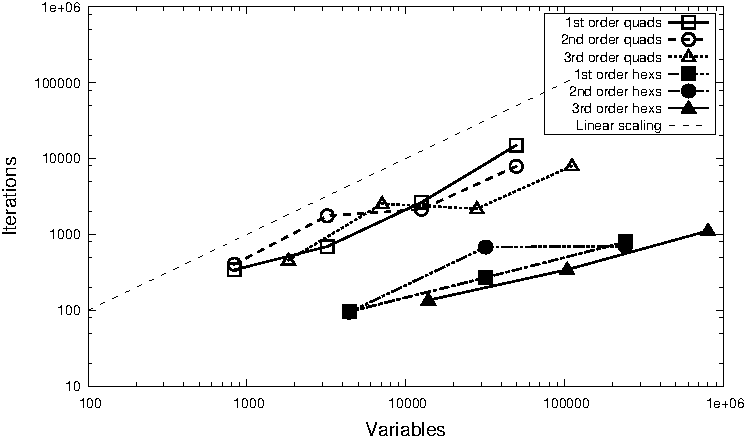
\includegraphics[scale=1.2]{FGaBP_itrs}
	}
	\caption{The \acrshort{acr:fgabp} algorithm executed on quadrilateral and hexahedral meshes of different orders.}
	\label{fig:fgabpItr}
\end{figure}


\subsection{Element Merging Performance}
\label{sec:elmMergRes}

The \gls{acr:em} feature implemented with the \gls{acr:fgabp} algorithm is demonstrated using a structured triangular mesh on a unit square domain.
The Laplace equation is solved in the domain using zero Dirichlet on the boundary.
The unit square is subdivided into equally spaced sub-squares where each square is further divided into two right triangles.
We perform two levels of merges by merging each two adjacent triangles, and then each four adjacent triangles.
The original mesh has $N_f=200000$ triangular element \glspl{acr:fn}.
Relaxation was not used in order to isolate the effect of merging on the iteration count.
The algorithm iterations were terminated when the message relative $l^2$-norm reached $<10^{-9}$.
\tableRef{tbl:fgabpMerge} shows the speedup results of the merges.
Execution was performed on an Intel Core2 Quad CPU with clock frequency of 2.83 GHz.


The merge results in increasing speedups.
Noting the overall computational complexity of the measured algorithm is approximately $\bigo{TN_f(n^3 + n^2)}$, where $T$ is the total number of iterations, the overall computational complexity of the merged algorithms has actually increased as can be noted by the complexity ratio column.
However, the execution time was actually faster which was mainly due to the improved locality of the algorithm. 
This improved locality results in better trade-offs of cache and memory bandwidth for cheaper CPU flops.

\begin{table}
	\centering
	\begin{threeparttable}
		\caption{AU-FGaBP with Element Merge Speedups.} \label{tbl:fgabpMerge}
		\begin{tabular}{lrrrr>{\itshape}r} \toprule
			Merge       & $N_f$  & $n$ & Iteration      & Complexity     & \gls{acr:su} \tabularnewline
			&        &      & ratio\tnote{1} & ratio\tnote{2} & \tabularnewline
			\midrule
			un-merged   & 200000 & 3    & 1.0            & 1.0            & 1.0 \tabularnewline
			2-triangle  & 100000 & 4    & 1.08           & 0.972          & 1.34 \tabularnewline
			4-triangle  & 50000  & 6    & 1.35           & 0.771          & 2.89 \tabularnewline
			\bottomrule
		\end{tabular}
		\begin{tablenotes}
			\begin{footnotesize}
			\item[1] {Iterations ratio = iterations of un-merged / merged.}
			\item[2] {Complexity ratio = complexity of un-merged / merged.}
			\end{footnotesize}
		\end{tablenotes}
	\end{threeparttable}
\end{table}


\section{Conclusion}
\label{sec_conclusion}

In this chapter, we presented the novel \gls{acr:fgabp} algorithm which performs inherently parallel \gls{acr:fem} computations element-by-element.
We presented a variational inference reformulation for the \gls{acr:fem} in order to facilitate the use of the \gls{acr:bp} computational inference algorithms.
The new probabilistic \gls{acr:femfg} model was introduced to address general \gls{acr:fem} problems which facilitates the derivation of various forms of the \gls{acr:fgabp} algorithm.
The approximate update and element merging variants of the \gls{acr:fgabp} algorithm were introduced which illustrates the \gls{acr:femfg} model flexibility in reducing computational complexity and improving the memory bandwidth utilization.
The \gls{acr:fgabp} algorithm was illustrated to solve the \gls{acr:fem} problem in parallel, element-by-element, eliminating the need for large sparse matrix operations.
The scale of the tested problems demonstrates that the algorithm is also suited for large-scale \gls{acr:fem} implementations on emerging parallel architectures.
The \gls{acr:fgabp} algorithm demonstrated significant scalability advantages in terms of both computation and memory bandwidth for increasing \gls{acr:fem} element order in both 2D and 3D domains.
In the following chapter, we will introduce a multigrid scheme for the \gls{acr:fgabp} that will significantly reduce its iteration count, which makes it competitive with state-of-the-are solvers such as the \gls{acr:mgpcg}.







%==========
\graphicspath{{figs/Chp-FMGaBP/}}

%%Fakesection Abstract
\glsreset{acr:fmgabp}


\chapter{Parallel Multigrid Adaptation for the Finite Element Gaussian Belief Propagation Algorithm}
\label{chp:FMGaBP}

%%Fakesection Abstract
In this chapter we introduce a novel parallel multigrid algorithm, referred to as the \gls{acr:fmgabp} algorithm, to accelerate the convergence of the previously introduced \gls{acr:fgabp} algorithm.
The \gls{acr:fmgabp} reduces the iteration count required for convergence to a competitive level while maintaining all the parallelism features of the original \gls{acr:fgabp} algorithm.
The \gls{acr:fmgabp} algorithm processes the \gls{acr:fem} computation in a fully distributed and parallel manner, with stencil-like element-by-element operations, while eliminating all global algebraic operations.
To our knowledge, this is the first multigrid formulation for continuous domain Gaussian \gls{acr:bp} type algorithms.
Similar to the \gls{acr:fgabp} algorithm, the \gls{acr:fmgabp} algorithm finds the solution to the variational formulation of the \gls{acr:fem} problem in a distributed manner.
In comparison with \gls{acr:mgpcg} solvers, the \gls{acr:fmgabp} algorithm demonstrates considerable iteration reductions as tested by Laplace benchmark problems.
In addition, the parallel implementation of the \gls{acr:fmgabp} algorithm shows a speedup of up to 2.9 times over the parallel implementation of \gls{acr:mgpcg} using eight CPU cores.


\section{Introduction}
The \gls{acr:pwgabp} algorithm, introduced by \cite{bib:Shental2008GBPSSLE,bib:Weiss01CorrectnessBelief}, was discussed in Chapters \ref{chp:PW-GaBP} and \ref{chp:relGaBP} illustrating great potential to parallelize the solving stage of the \gls{acr:fem} \cite{bib:El-Kurdi2012EIOGBPSFLSDDLS,bib:El-Kurdi2012RGBP}.
In addition, \gls{acr:pwgabp} has been shown to outperform classical iterative solvers such as \gls{acr:gs} and Jacobi \cite{bib:Shental2008GBPSSLE}.
However such algorithms, which are derived based on pairwise interconnect assumptions on the underlying \gls{acr:gm}, suffer mostly from a lack of convergence when diagonal dominance properties are not met.
In \chpRef{chp:FGaBP}, the \gls{acr:fgabp} algorithm was introduced which addresses the convergence shortcomings of \gls{acr:pwgabp} and improves the parallel efficiency of the \gls{acr:fem} computation.
While the \gls{acr:fgabp} was demonstrated to efficiently solve \gls{acr:fem} problems in parallel, element-by-element; however the \gls{acr:fgabp}'s convergence rate tends to stall when executed on fine meshes.


In this work we address this issue by introducing the novel \gls{acr:fmgabp} algorithm.
Our results for various scheduling versions of \gls{acr:fmgabp} demonstrate high convergence rates independent of the scale of discretization on the finest mesh.
In addition, we show for a benchmark Laplace problem that the \gls{acr:fmgabp} requires, in certain cases, less iterations than the \gls{acr:mgpcg} solver.
The eight thread multicore implementation of \gls{acr:fmgabp} demonstrates speedups of up to 2.9 times over the \gls{acr:mgpcg} solver based on sparse algebraic operations as implemented by the multithreaded library \libName{deal.II}~\cite{bib:dealii2007}.


The chapter is organized as follows.
In \secRef{sec:fmgabp} we present the detailed formulation of the \gls{acr:fmgabp} algorithm.
Then in \secRef{sec:fmgabpImp} we present the implementation details of the \gls{acr:fmgabp} algorithm.
Finally in \secRef{sec:FMGaBP_res} we conclude with numerical and performance results and discussions.


\section{The FMGaBP Algorithm}
\label{sec:fmgabp}

Multigrid acceleration schemes \cite{bib:Trottenberg2001M,bib:Briggs2000AMT} provide optimal convergence speeds resulting in a number of iterations almost independent of the discretization level of the \gls{acr:fem} mesh.
It is expected that the \gls{acr:fgabp} algorithm can benefit greatly from multigrid schemes mainly because, \gls{acr:bp} communications on coarser levels can serve as bridges to communications between far away nodes on finer levels.
This has the effect of considerably improving the propagation of information in the \gls{acr:femfg} model and hence speeding up the overall convergence.
In this section, we introduce an efficient adaptation of multigrid schemes to the \gls{acr:fgabp} algorithm resulting in the \gls{acr:fmgabp} algorithm.
As will be shown later, the resulting \gls{acr:fmgabp} algorithm demonstrates convergence rates independent of the \gls{acr:fem} domain's discretization level.
In addition, the \gls{acr:fmgabp} retains the distributed nature of computations, which has important implications for \gls{acr:hpc} implementations. 
Mainly, the \gls{acr:fmgabp} level transfer operations are computationally decoupled and localized without requiring any global sparse algebraic operations.


The \gls{acr:fmgabp} algorithm considerably improves the \gls{acr:fgabp} convergence rate while maintaining high parallel efficiency of stencil-like, element-by-element, operations.
Our results will later demonstrate that not only the \gls{acr:fmgabp} shows considerable advantage in parallel efficiency, but also, compared to the \gls{acr:mgpcg}, the \gls{acr:fmgabp} shows iteration reductions in certain cases.
The distinguishing feature of the \gls{acr:fgabp} algorithm is solving the \gls{acr:fem} in parallel, element-by-element, without assembling a large sparse matrix or performing any global algebraic operations such as \glspl{acr:smvm}.
This key advantage, which has important impacts on parallel hardware implementations, is maintained by the new multigrid formulation for \gls{acr:fmgabp}.


\subsection{Hierarchical Mesh Refinement}


A brief overview of multigrid schemes was presented in \secRef{sec:RMG}.
In our derivation of the \gls{acr:fmgabp} algorithm, we will be considering \gls{acr:gmg} schemes with hierarchical meshes.
In hierarchical mesh refinement schemes, local element splitting is used to generate a hierarchy of multigrid levels.
As an example, \figRef{fig:split} shows hierarchical refinement by starting from an initial coarse triangular mesh and then splitting each triangle into four geometrically similar child triangles by inserting nodes at midpoints of the parent triangle's edges.
Similar refinement can be used for quadrilateral and hexahedral meshes, where each quadrilateral (parent) is split into four child-quadrilaterals and each hexahedron (parent) is split into eight child-hexahedrons.
Each level of the hierarchy will be represented by a unique \gls{acr:femfg} graph; as will be shown later, the transfer operations will only occur between the factor nodes of the corresponding parent-child elements.
In addition, this hierarchical refinement scheme will provide key advantages for element-by-element parallel behavior of the \gls{acr:fmgabp}.
Also, by utilizing semi-irregular mesh hierarchies, more adaptation to arbitrary domains can be achieved than by using only structured meshes hierarchies.


However, and more importantly, the choice of the hierarchical refinement is not due to any imposed limitations from the \gls{acr:fmgabp} algorithm, but rather, it is used as an initial proof-of-concept phase to better illustrate the new \gls{acr:fmgabp} algorithm.
One approach to handle geometries with fine and complex features is to use non-conforming adaptive refinement \cite{bib:Becker2001AOCAAPEEFEM,bib:Bangerth2003AFEMDF} which will require special care to handle the non-conforming grid points.
In addition, adaptive refinement schemes rely on computing error estimations from a local element-by-element perspective which makes formulating the \gls{acr:fmgabp} for such refinement schemes an interesting future research direction.


\subsection{The Factor Node Belief}

To illustrate the \gls{acr:fmgabp} formulation, we start by defining a multivariate distribution, associated with each individual \fn{a}, referred to as the factor node belief $b_a(U_a)$, denoted for short as \fnb{a}.
The belief \fnb{a} function takes the form:
\begin{equation}
	b_{a}^{(t)}(U_{a}) \propto \Psi_{a}(U_{a}) \prod_{i\in\mathcal{N}(a)}\eta_{ia}^{(t)}(U_{i}), \label{eqn:genFB}
\end{equation}
where $U_a$ is the vector of random unknowns linked to \fn{a}.
In essence the belief \fnb{a}, in contrast with the nodal belief \vnb{i} as defined in \eqnRef{eqn:genB}, represents the marginal distribution as seen from \fn{a} in a particular iteration $t$.
When we use the \gls{acr:femfg} setting, the factor belief $b_a$ takes a Gaussian multivariate form as:
\begin{equation}
	b_{a}^{(t)}(U_a) \propto\exp\left[-\frac{1}{2}U_{a}^{T}W_{a}^{(t)}U_{a}+(K_{a}^{(t)})^{T}U_{a}\right] \label{eqn:gaussFB}
\end{equation}
where the parameters $W_a$ and $K_a$ represent the inverse covariance and the source vector of the factor node respectively.
Note that the function \fnb{a} takes an iterative form, where the matrix $W_a$ and the vector $K_a$ are updated each iteration according to the \gls{acr:fgabp} update rules in (\ref{eqn:fWK}).


By observing the dynamics of the message update rules of the \gls{acr:bp} algorithm in (\ref{eqn:genFNUM}), (\ref{eqn:genVNUM}), and (\ref{eqn:genB}), we can show that at message convergence the joint mean vector of \fnb{a}, given by $W_{a}^{-1}K_a$ as computed locally from the factor node's perspective, will be equal to the marginal means of $U_a$ as computed from the nodal perspective by (\ref{eqn:vnm}).
That is, if we form a vector of nodal marginal means as computed by the \gls{acr:fgabp} rule \eqnRef{eqn:vnm} in the vector $\bar{\mu}_a$ for the set of nodes connected to \fn{a}, then at message convergence we obtain:
\begin{align}
	\bar{\mu}_a & = \left[\mu_{\mathcal{L}(j)}\right],\,\,\text{where } j\in\mathcal{N}(a)\\
	& = W_{a}^{-1}K_a \label{eqn:fpMarj}
\end{align}
and $\mathcal{L(\cdot)}$ is the mapping of global variable node indices to local factor node indices.


In order to demonstrate this result, we start by formulating the marginal for $U_i$, denoted as $\tilde{b}_{i}(U_{i})$, from the defined \fnb{a} using the general \gls{acr:bp} message communication as follows:
\begin{align}
	\tilde{b}_{i}^{(t)}(U_{i})& \propto\underset{U_{\mathcal{N}(a)\setminus i}}{\int} b_{a}^{(t)}(U_{a})\ \mathrm{d}U_{\mathcal{N}(a)\setminus i}\\
	& \propto\underset{U_{\mathcal{N}(a)\setminus i}}{\int}\Psi_{a}(U_{a})\prod_{j\in\mathcal{N}(a)}\eta_{ja}^{(t)}(U_{j})\ \mathrm{d}U_{\mathcal{N}(a)\setminus i}.
\end{align}
Since at $j=i$, $\eta_{ia}(U_{i})$ is a function of the single variable node $U_i$, hence we can take it outside the integral as:
\begin{equation}
	\tilde{b}_{i}^{(t)}(U_{i}) \propto \eta_{ia}^{(t)}(U_{i})\underset{U_{\mathcal{N}(a)\setminus i}}{\int}\Psi_{a}(U_{a})\prod_{j\in\mathcal{N}(a)\setminus i}\eta_{ja}^{(t)}(U_{j})\ \mathrm{d}U_{\mathcal{N}(a)\setminus i}.
\end{equation}
Here, we are considering the case where all the \gls{acr:bp} messages are stationary, then we can substitute the \gls{acr:bp} update rules \eqnRef{eqn:genFNUM}, \eqnRef{eqn:genVNUM} and \eqnRef{eqn:genB} which results in:
\begin{align}
	\tilde{b}_{i}^{(t)}(U_{i}) & \propto\left[\prod_{k\in\mathcal{N}(i)\setminus a}m_{ki}^{(t)}(U_{i})\right]m_{ai}^{(t)}(U_{i})\\
	& \propto\prod_{k\in\mathcal{N}(i)}m_{ki}^{(t)}(U_{i})\\
	& \propto b_{i}^{(t)}(U_{i}).
\end{align}
The above result states that, at message convergence the marginal of a particular variable node computed using a factor belief function is equivalent to the marginal distribution of that node computed from the nodal perspective incorporating global information as in \eqnRef{eqn:vnm}.
Now, since for multivariate Gaussian distributions the marginal mean of a variable is equal to its corresponding value in the joint mean vector; therefore, at message convergence, the Gaussian means as computed from the local belief perspective will be in agreement with the marginal means as computed from global perspective as stated in \eqnRef{eqn:fpMarj}.

\subsection{Local Belief Residual-Correction}
Given the belief condition in \eqnRef{eqn:fpMarj}, then for each factor on a fine grid we can formulate a quantity referred to as the belief residual $r_a$ given by:
\begin{equation}
	r_a^{(t)} = K_a^{(t)} - W_a^{(t)} \bar{\mu}_a^{(t)} \label{eqn:br}.
\end{equation}
When hierarchical mesh refinement is used, the belief residuals of each group of child elements can locally be restricted into the parent element as:
\begin{equation}
	K^H_a =\mathcal{R}_l r^{h}_a \label{eqn_rr}
\end{equation}
where $K^H_a$ is the source vector of the parent element, $r^{h}_a$ is the accumulated local residual of child elements, and $\mathcal{R}_l$ is the child-parent local restriction operator.
Notice that we dropped the iteration count $(t)$ since we are operating in the same iteration for both sides of the equations.


Similarly, we can use local interpolation operations in order to apply the corrections from the coarse elements as follows:
\begin{equation}
	\bar{\mu}_a^h \gets \bar{\mu}_a^h + \mathcal{I}_l \bar{\mu}_a^H.
\end{equation}
Using the level updated $\bar{\mu}_a^h$ we can reinitialize the corresponding level local messages using again \eqnRef{eqn:br} but with $r_a \to 0$, then solving for the local factor messages as follows:
\begin{align}
	K_a^h & = W_a \bar{u}_a^h\\
	\mathcal{B}_a^h & = K_a^h - B_a^h. \label{eqn:messCorr}
\end{align}


Since we are only considering linear problems, the $\alpha$ messages are only dependent on the factor matrices which are not affected by the residual-correction multigrid scheme.
Therefore, the $\alpha$ messages retain their previous value on each level transfer.
It was found by experimentation on first order \gls{acr:fem} problems, that the $\mathcal{R}_l$ is typically the transpose of $\mathcal{I}_l$ up to a constant factor as follows:
\begin{equation}
	\mathcal{R}_l = c \left(\mathcal{I}_l\right)^T \label{eqn:galerkinCnd}
\end{equation}
where $c$ was found to equal to $1$ for structured quadrilateral and hexahedral meshes, while it was equal to $\frac{1}{3}$ for semi-irregular triangular meshes.


\subsection{Local Transfer Operations}
The \gls{acr:fmgabp} local transfer operations can be enhanced by the definition of local node numbering schemes between each set of parent-child elements.
The parent-child numbering scheme facilitates the transfer of residuals from child nodes to parent nodes using logical index computations.
As a result, the \gls{acr:fmgabp} transfer operations take the form of local stencil-like operation.
\figRef{fig:quadTrans} shows the residual transfer operations from one child node to the corresponding parent nodes using a particular local numbering scheme.
The local transfer scheme can be generalized to 3D meshes.
For example, when refining a hexahedron into eight hexahedrons, the nodes on the faces of the refined hexahedron will have weightings similar to the ones illustrated in \figRef{fig:quadTrans}, while the node in the interior will have a weighting equal to $\frac{1}{8}$.
In the case of triangular and tetrahedral meshes, the nodal weights will consist of $1$ and $\frac{1}{2}$ only.

\begin{figure}
	\centering
	{
	\subfloat[Child-a]{%
	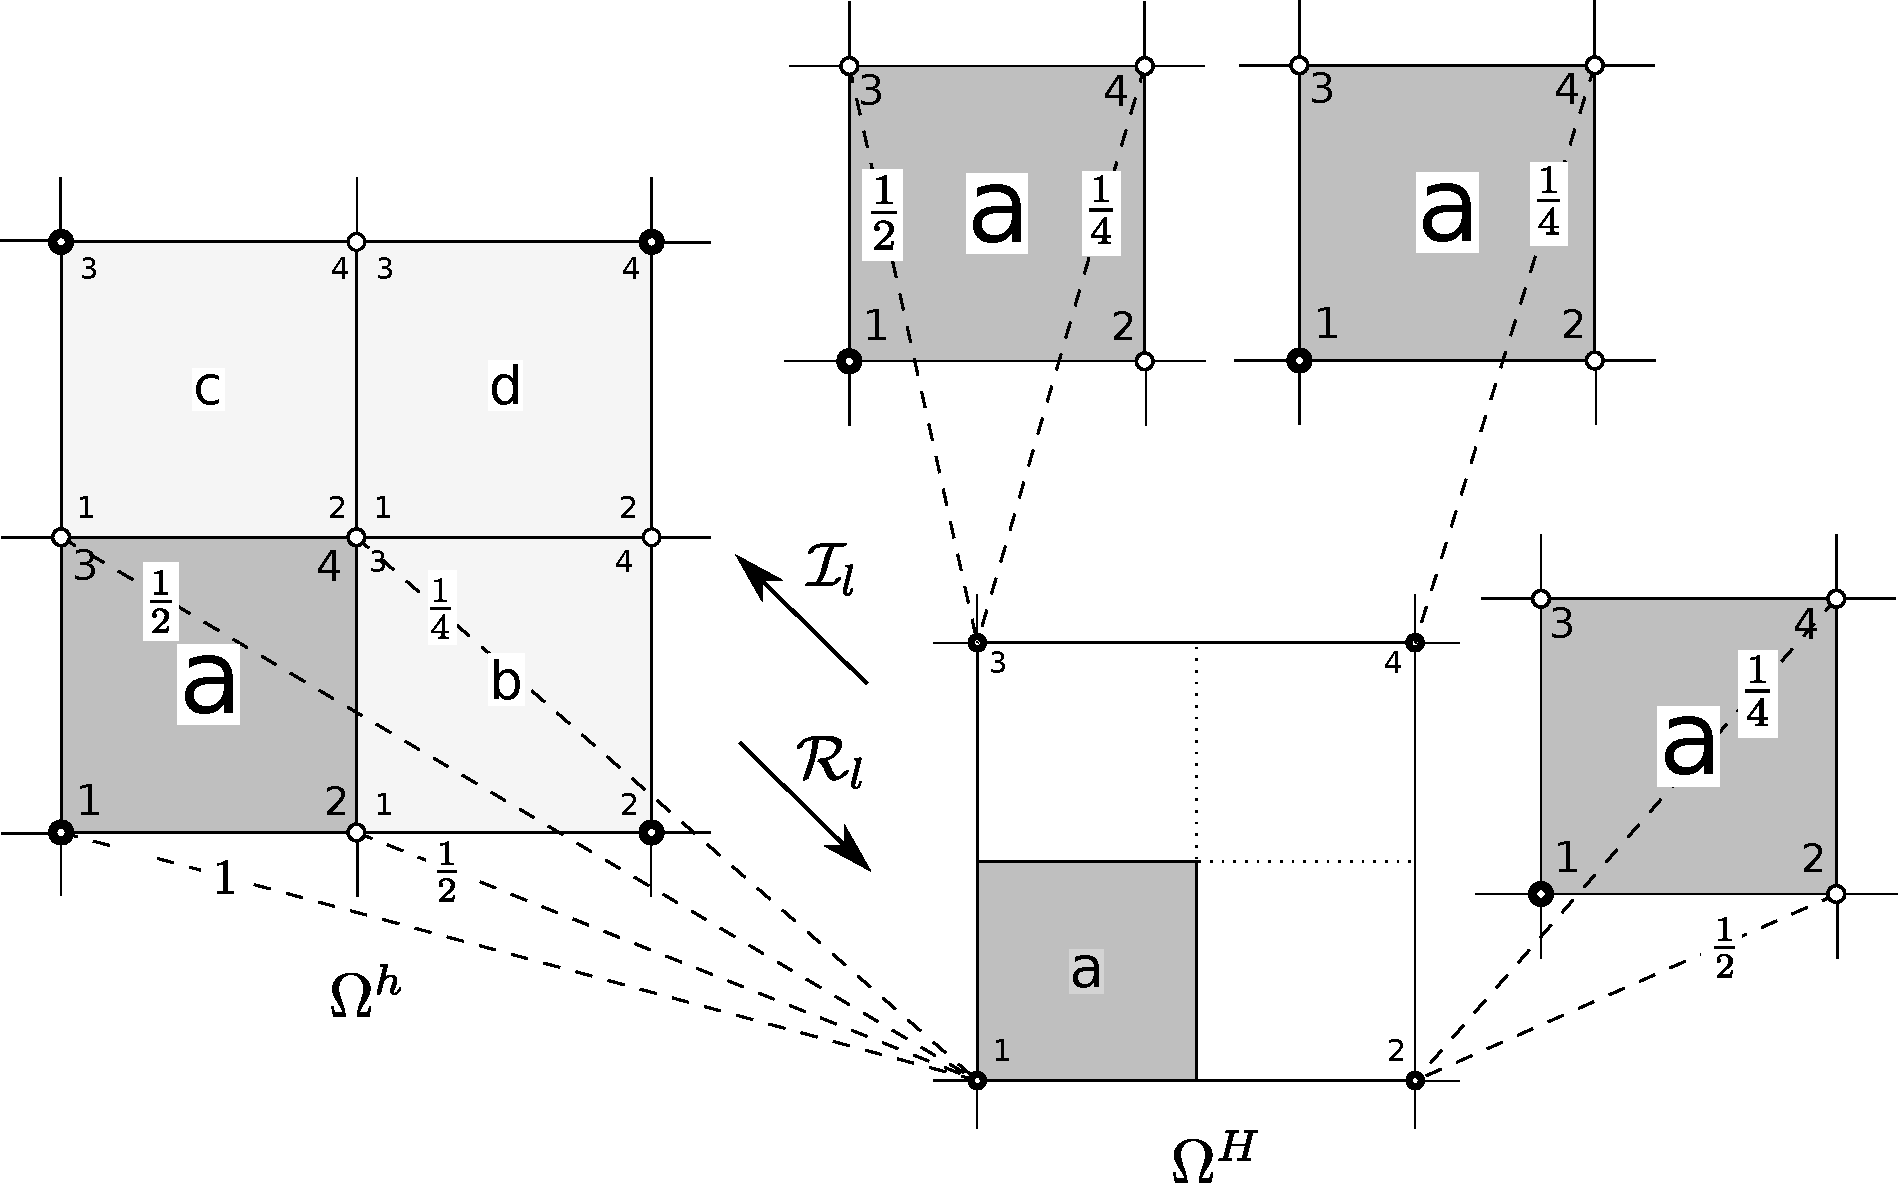
\includegraphics[scale=.4]{quad_trans_a} \label{fig:quadTrans_a}
	}
	\vfil
	\subfloat[Child-d]{%
	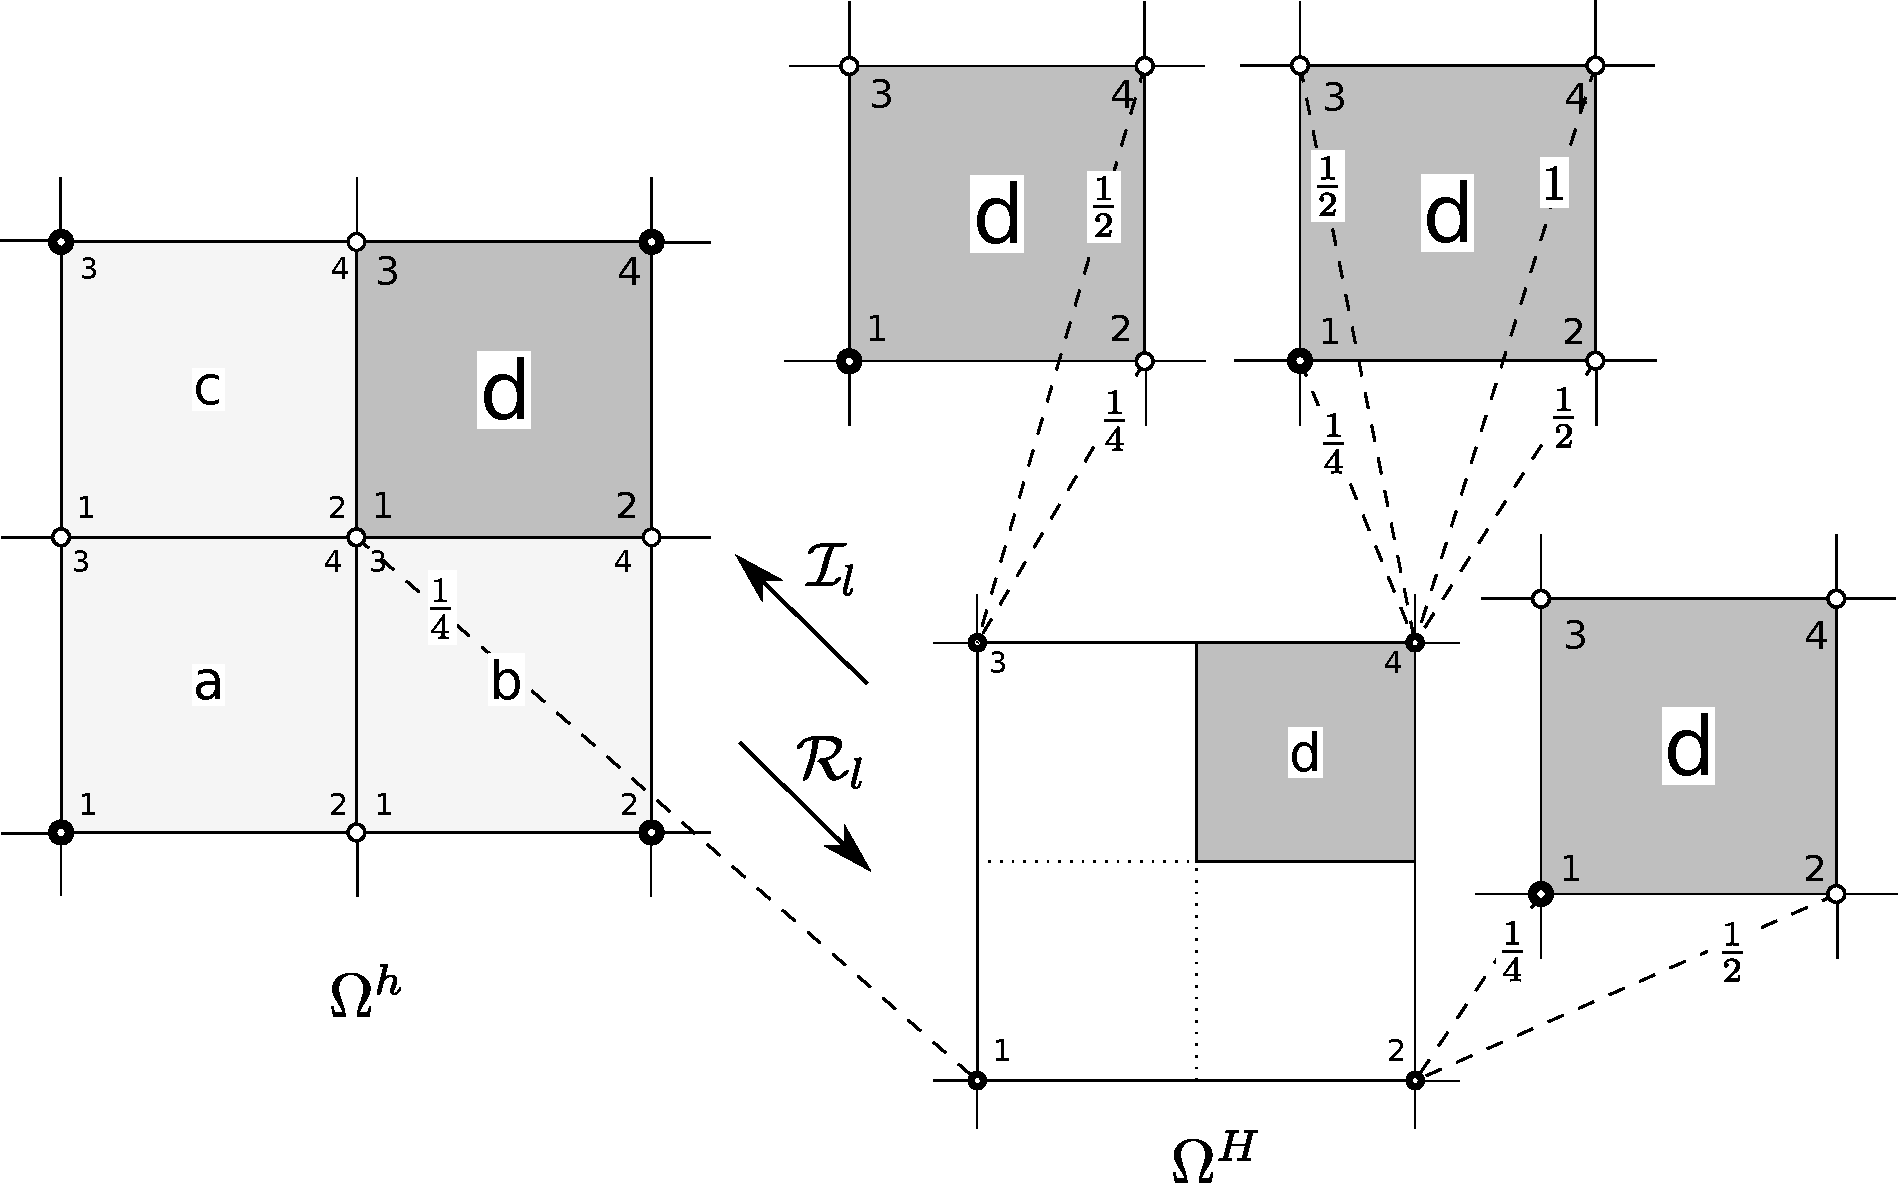
\includegraphics[scale=.4]{quad_trans_d} \label{fig:quadTrans_d}
	}
	}
	\caption[The \acrshort{acr:fmgabp} local transfer operations.]{\gls{acr:fmgabp} local transfer weights between two example child elements and the corresponding parent element. \protect\subref*{fig:quadTrans_a}~Local transfer weights for child-a. \protect\subref*{fig:quadTrans_d}~Local transfer weights for child-d.}
	\label{fig:quadTrans}
\end{figure}

Finally, It is important to note that the local \gls{acr:fmgabp} transfer operations between each set of parent-child elements create parallel operations that are also thread-safe.
This means that these local transfer operations can be implemented in an embarrassingly parallel stencil-like operations.

\subsection{The Global Residual and the Local Belief Residuals}

To illustrate the relationship between the local belief residuals and the global residual, we start by assembling a global residual vector $r_{\mathcal{G}}$ by summing all the local residual components from each factor node as follows:
\begin{equation}
	r_{\mathcal{G}} = \sum_{a \in \mathcal{S}} r_a \label{eqn:glbResSum}
\end{equation}
where $\mathcal{S}$ is the set of all factor nodes.  
Note that the sum in \eqnRef{eqn:glbResSum} is carried out by resolving mappings from local factor indices to global indices.
In the following formulas, we consider this mapping to be implicitly stated in the sum form.
Also in order to define the residual for a particular \gls{acr:bp} iteration, we assume a synchronous schedule for message communications.
This does not lead to any loss of generality, but rather it greatly simplifies the formulation since other forms of schedules may not have a clearly definable iteration.
Alternatively, one way to represent iterations is to define an iteration for every single message update.
For such a case, our formulation will also hold.

Next we substitute the local belief residual \eqnRef{eqn:br} into \eqnRef{eqn:glbResSum} to get:
\begin{align}
	r_{\mathcal{G}} & = \sum_{a \in \mathcal{S}} \left[ K_a - W_a \bar{\mu}_a \right]\\
	& = \sum_{a \in \mathcal{S}} \left[ B_a +\mathcal{B}_a - M_a \bar{\mu}_a - \mathcal{A}_a \bar{\mu}_a \right]\,\,\, \text{substituting \eqnRef{eqn:fWK}}.
\end{align}
Note that the terms $\sum_{a \in \mathcal{S}} B_a $ and $\sum_{a \in \mathcal{S}} M_a \bar{\mu}_a$ represent the assembly of the global system $f$ and $A\bar{\mu}$ correspondingly, then we have:
\begin{equation}
	r_{\mathcal{G}} = f - A\bar{\mu} + \sum_{a \in \mathcal{S}} \left[ \mathcal{B}_a -  \mathcal{A}_a \bar{\mu}_a \right] \label{eqn:glbResMess}
\end{equation}
where the dimensions of the system $A$ and $f$ are $N$, where $N$ is the total number of unknowns; and $\bar{\mu}$ is a vector of the same dimension representing the solution estimate obtained from the current \gls{acr:fgabp} level iteration.
Recall that $\mathcal{B}_a$ and $\mathcal{A}_a$ represent the factor node's incoming messages as in \eqnRef{eqn:fWK} where the incoming messages $\alpha_{ia}$ and $\beta_{ia}$ can each be substituted by \eqnRef{eqn:vna} and \eqnRef{eqn:vnb} correspondingly, then we can assemble $\mathcal{B}_a$ and $\mathcal{A}_a$ as follows:
\begin{align}
	\sum_{a \in \mathcal{S}}\mathcal{A}_a & = C \mathcal{A}_{\mathcal{G}} \label{eqn:glbA}\\
	\sum_{a \in \mathcal{S}}\mathcal{B}_a & = C \mathcal{B}_{\mathcal{G}} \label{eqn:glbB}
\end{align}
where $\mathcal{A}_{\mathcal{G}}$ is a diagonal matrix with dimension $N\text{-by-}N$ and off-diagonals equal to zero, where $N$ is the total number of unknowns; $\mathcal{B}_{\mathcal{G}}$ is a global vector of the same dimension; and $C$ is a diagonal matrix of the same dimension with constant diagonals that will be clarified shortly.
The diagonal of $\mathcal{A}_{\mathcal{G}}$ contains the nodal values $\alpha_i$ which are basically the sum of incoming $\alpha$ factor messages as in \eqnRef{eqn:vnaSum}; and similarly, the vector $\mathcal{B}_{\mathcal{G}}$ contains the sum of incoming $\beta$ factor messages as in \eqnRef{eqn:vnbSum}.
Each diagonal element of $C$ is equal to the corresponding nodes' number of links minus one.

It is easier to illustrate the assembly of $\mathcal{A}_{\mathcal{G}}$, $\mathcal{B}_{\mathcal{G}}$, and $C$ using the example diagram shown in \figRef{fig:nodalAssembly}.
If we are to assemble node index $i$ of $\mathcal{A}_{\mathcal{G}}$, then we would effectively sum all the corresponding diagonal values of $\mathcal{A}_a$, $\mathcal{A}_b$, \ldots up to $\mathcal{A}_f$, which results in:
\begin{align}
	\left[ C \mathcal{A}_{\mathcal{G}} \right]_i & = \sum_{k \in \mathcal{N}(i)} \left[ \mathcal{A}_k \right]_i\\
	& = c \alpha_i - \sum_{k \in \mathcal{N}(i)} \alpha_{ik}\\
	& = l \alpha_i - \alpha_i , \,\,\, \text{substituting \eqnRef{eqn:vnaSum}} \\
	& = (l-1) \alpha_i
\end{align}
where $l = 6$ is the number of \gls{acr:femfg} links around node $i$.
Similarly, we can perform the assembly for $\mathcal{B}_{\mathcal{G}}$.
\begin{figure}
	\centering
	{
	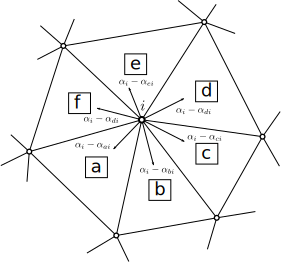
\includegraphics[scale=1.0]{glb_res}
	}
	\caption{The outgoing messages around an interior node $i$ in \acrshort{acr:femfg}.}
	\label{fig:nodalAssembly}
\end{figure}


Now substituting \eqnRef{eqn:glbA} and \eqnRef{eqn:glbB} into \eqnRef{eqn:glbResMess} we obtain:
\begin{equation}
	r_{\mathcal{G}} = f - A\bar{\mu} +  C \mathcal{B}_{\mathcal{G}} - C \mathcal{A}_{\mathcal{G}} \bar{\mu}. \label{eqn:glbResMess_2}
\end{equation}
Noting that $C \mathcal{A}_{\mathcal{G}} \bar{\mu} = C \mathcal{B}_{\mathcal{G}}$, since $[\bar{\mu}]_i = \beta_i / \alpha_i\,\,\forall i$, then \eqnRef{eqn:glbResMess_2} reduces to:
\begin{align}
	r_{\mathcal{G}} & = f - A\bar{\mu} +  C \mathcal{B}_{\mathcal{G}} - C \mathcal{B}_{\mathcal{G}}\\
	& = f - A\bar{\mu}.
\end{align}
This result illustrates that minimizing the local belief residuals is equivalent to minimizing the global residual for the assembled linear system $Au=f$, albeit computed in a distributed way without needing to assemble the sparse matrix $A$.
The result also shows that the local distributed computations performed by the \gls{acr:fmgabp} algorithm amounts to solving the same problem from global perspectives.
The reader at this point might raise the question whether it will be possible to decompose the global residual into local quantities.
In fact, such a decomposition would be hard; since without any prior knowledge of the local messages per each iteration, the decomposition would not be unique.


\subsection{The FMGaBP Fixed-Point}
Clearly from \eqnRef{eqn:br}, once all messages converge on the fine grid, that is once $\bar{\mu}_a^h \to \left[ u_0 \right]_a$ where $\left[ u_0 \right]_a$ is the true solution vector of the local nodes of $a$, then $r_a \to 0$.
Furthermore, by uniqueness of the \gls{acr:fem} solution on coarser grids, at stationarity the $\beta$ messages on each subsequent coarse grid will also be zero, hence the correction $\bar{u}_a^H$ from the coarser grids will consequently be zero.
Therefore, the \gls{acr:fmgabp} is a fixed-point algorithm for the true solution on the fine grid.

\subsection{The FMGaBP Algorithm Listing}

\algRef{alg:fmgabp} illustrates a high-level listing of the \gls{acr:fmgabp} algorithm.
The \gls{acr:fmgabp} algorithm can be seen as executing instances of the \gls{acr:fgabp} algorithm on each level in the multigrid hierarchy.
The loops on lines \ref{alg:fmgabpDownV} and \ref{alg:fmgabpUpV} traverse all the levels on the V-cycle except the coarsest level, first going down the cycle and then up the cycle.
Each level visited, the \gls{acr:fgabp} executes $v_1$ iterations down the cycle and $v_2$ iterations up the cycle.
It was found that $v_1 = v_2 =1$ is typically sufficient in most cases.
We iterate on the coarsest level using the \gls{acr:fgabp} algorithm, that is in contrast to conventional multigrid methods where a direct solver is used on the coarsest level.
Since the coarsest level contains a very small number of factors, within the order of few hundreds, its execution can be quite fast.
Also as can be noted on Line \ref{alg:fmgabpCrs}, there was no need to use a low tolerance on the coarsest level.
In many cases also, a tolerance of $10^{-6}$ was found to be sufficient on the coarsest level.
One important note to make is that the \gls{acr:fmgabp} algorithm can solve the problem down to machine floating-point precision, as can be noted by the low tolerance for convergence on Line \ref{alg:fmgabpTestTol}.

\begin{algorithm}[t]
  %\centering
	\begin{algorithmic}[1]
		\STATE Obtain \gls{acr:fem} hierarchical mesh
		\LOOP[For each level in the mesh hierarchy]
		\STATE Perform partition-color
		\STATE Generate element matrices $M_s$ and source vectors $B_s$ 
		\STATE Incorporate boundary conditions 
		\STATE \textit{Initialize:} $\alpha_{ij} = 1,\,\, \beta_{ij} = 0,\,\,\forall i,j$
		\AlgENDLOOP
		\REPEAT[\gls{acr:fmgabp} V-cycle iteration: $t=1,2,\cdots$]
		\LOOP[Traverse levels down the V-cycle] \label{alg:fmgabpDownV}
		\IF{Coarsest level reached}
		\STATE Exit
	\ENDIF
	\STATE Execute $v_1$ iterations of \gls{acr:fgabp} (\algRef{alg:FGaBP})
	\STATE Restrict residuals from child-factors into parent-factors
	\AlgENDLOOP
	\STATE Execute \gls{acr:fgabp} on coarsest level for tolerance  $<10^{-9}$ \label{alg:fmgabpCrs}
	\LOOP[Traverse levels up the V-cycle] \label{alg:fmgabpUpV}
	\STATE Prolongate corrections from parent-factors into child-factors
	\STATE Execute $v_2$ iterations of \gls{acr:fgabp} (\algRef{alg:FGaBP})
	\AlgENDLOOP
	\UNTIL{Convergence check on finest level messages for tolerance  $<10^{-16}$} \label{alg:fmgabpTestTol}
	\STATE \textit{Output:} $\mu_i = \frac{\beta_i}{\alpha_i}$
\end{algorithmic}
\caption{The \acrshort{acr:fmgabp} algorithm.}
\label{alg:fmgabp}
\end{algorithm}

\section{Implementation}
\label{sec:fmgabpImp}

\subsection{Data-Structures}

The \gls{acr:fmgabp} data-structures are mostly based on the \gls{acr:fgabp} data-structures with the addition of another dense matrix per multigrid level.
The added matrix stores the index associations of parent-child \glspl{acr:fn} for each hierarchical pair of coarse-fine levels.
The total size of the \gls{acr:fmgabp} data-structure can be obtained by:
\begin{align}
	\mathrm{FMGaBP\, Memory} & \approx O\left[ (Z+cN_f) \sum_{l=0}^{L-1} \frac{1}{c^l} - cN_f \right]\\
	& = O\left[(Z+cN_f) \frac{1-(1/c)^{L}}{1-(1/c)} - cN_f\right]
	\label{eqn:fmgabpMem}
\end{align}
where $l$ is the level index; $L$ is the total number of levels; $Z=2 \gls{acr:nv}+\gls{acr:nf}(n^2+4n)$ which is the \gls{acr:fgabp} memory on the finest level as detailed in \secRef{sec:fgabpDS}; and $c$ is the number of children, e.g. $c=4$ for 2D quadrilateral meshes or $c=8$ for 3D hexahedral meshes.
Clearly, the overall memory complexity is linear in \gls{acr:nv} as $L\to \infty$.

\subsection{Multicore CPU Implementation}

Similar to the \gls{acr:fgabp}, the \gls{acr:fmgabp} code was designed using C++ \gls{acr:oop} \cite{bib:c++stroustrup2013,bib:c++prata2004}.
This facilities the integration of the \gls{acr:fgabp} code as a level solver into the \gls{acr:fmgabp} with minimal recoding.
In addition, different \gls{acr:fem} open-source libraries, such as \dealName{} \cite{bib:dealii2007} and \libName{GetFEM++} \cite{bib:getfem}, can be integrated easily which enables thorough testing of the \gls{acr:fmgabp} algorithm.
The library \libName{GetFEM++} was used to test our code using irregular triangular meshes that are generated by \libName{Gmsh} \cite{bib:gmsh2009}, while \dealName{} was used to test our code on quadrilateral and hexahedral meshes.
However out of the two, only \dealName{} provides parallel implementation of its solver and therefore it will be used for our performance analysis.
While there are other high quality C++ \gls{acr:fem} libraries such as \libName{Dune} \cite{bib:dunefemwebpage,bib:dunefemwebpage} and \libName{libMesh} \cite{bib:libMesh}, \dealName{} and \libName{GetFEM++} were the most up-to-date with extensive documentation and active support teams.


Another advantage of using \gls{acr:oop} style coding is that the \gls{acr:fmgabp} implementation performance can be tested using different \gls{acr:blas} libraries and dense solvers \cite{bib:blas,bib:blasDongarra:2002,bib:lapack}.
These libraries are needed by the \glspl{acr:fn} for the efficient execution of its dense operations, such as the Cholesky inversion or the \gls{acr:gs} iteration required by the \gls{acr:aufgabp} scheme.
For that purpose, we used different dense routines from the libraries \dealName{}, \libName{gmm} \cite{bib:gmm}, and \libName{Eigen} \cite{bib:eigen}.
\libName{Eigen}, however, seemed to produce the best overall results.


Similar to the \gls{acr:fgabp} code, the \gls{acr:fmgabp} code was parallelized using \libName{OpenMP} \cite{bib:openmp}.
Each thread is assigned to handle the transfer operations of each parent-child \glspl{acr:fn} set.
The transfer operations are fully decoupled; and hence, there was no need for the use of elaborate partitioning schemes such as coloring in order to ensure thread-safety.
A single thread synchronization directive is used at the end of each transfer operation either restriction or prolongation.
Finally, the output solution was visualized using \libName{Paraview} \cite{bib:paraview}.



\subsection{Manycore GPU Implementation}

In the past decade, architectures with many (tens or hundreds of) integrated cores have been introduced and used in the scientific computing community.
\Glspl{acr:gpu} are a popular class of manycore processors offering greater opportunities of parallelism on a single chip than multicore CPUs.
It is expected that adeptly parallel algorithms such as the \gls{acr:fmgabp} can benefit from the increased parallelism of \gls{acr:gpu} architectures.
In this section, we will detail the implementation techniques used to evaluate the \gls{acr:fmgabp} performance on \gls{acr:gpu} architectures.

\subsubsection{Background on GPUs}

Attempts to port parts or all of the \gls{acr:fem} computations to manycore architectures have been presented in previous works.
Most of these works are aimed at accelerating either the global sparse matrix assembly or the global system solve stage.
Constrained by the special characteristics of their applications, the works in \cite{bib:Bolz2003SMSGPUs,bib:rodriguez2006NSM} present simple assembly strategies suited for manycore architectures.
Their proposed techniques are not applicable for general \gls{acr:fem} applications but, rather, are mostly suited to the sparsity structure of their specific applications.
Graph coloring schemes in \cite{bib:Komatitsch2009PHF,bib:Hesthaven2007NDG,bib:Cris2011assemblyGPU} are used to partition the \gls{acr:fem} elements to non-overlapping sets, in order to enable a parallel thread-safe execution of the assembly routines for the global sparse matrix.
Assembling a global sparse matrix, to be solved in a separate stage, based on graph coloring and partitioning can be costly.
For the \gls{acr:fgabp} algorithm, coloring adds little overhead since the global sparse matrix is never assembled and coloring is used, rather, to compute the \gls{acr:fem} solution in parallel.
Other work \cite{bib:Dziekonski2013generation,bib:Dziekonski2012finite,bib:Fu2014architecting} propose strategies and novel sparse storage formats to reduce the memory footprint of the assembled sparse matrix.
Since, \gls{acr:fgabp} eliminates the need for assembling a large sparse matrix, many of the optimizations proposed in previous work are, thus, not applicable to our work.

Significant research has been aimed at improving the solve stage for sparse systems using \glspl{acr:gpu}.
Most these works focus on accelerating the execution of the compute intensive kernels in the Krylov solvers.
As shown in \cite{bib:Hoemmen2010EECS,bib:Mehridehnavi2013CAGPU} such efforts are mainly communication bound and are limited by the maximum performance achieved from parallelizing the compute intensive kernels.
The assembled matrix is usually large and sparse and in many cases does not fit in the small and fast access memory levels of CPU and the co-processor memory.


\gls{acr:fgabp} avoids assembling a global sparse matrix and, thus, is a promising candidate for manycore architectures.
Instead of solving a large sparse matrix, each \gls{acr:fgabp} iteration needs to compute the incoming and outgoing messages for each factor node.
The compute intensive kernel in a \gls{acr:fgabp} iteration involves computing the inverses of many small dense matrices; an operation that is embarrassingly parallel and well suited for manycore architectures.
Coloring the \gls{acr:femfg} models improves the underlying parallelism significantly and allows \glspl{acr:fn} of the same color to be processed in parallel by hundreds of threads without causing any synchronization or memory collisions when accessing the \gls{acr:vn} data.
To demonstrate the embarrassingly parallel nature of both the \gls{acr:fgabp} and \gls{acr:fmgabp} algorthims, we have implemented them on the {NVIDIA} Tesla {C2075} \gls{acr:gpu}.


\subsubsection{The GPU architecture}

The {NVIDIA} Tesla {C2075} \gls{acr:gpu}, which belongs to the Fermi generation, is used to illustrate the performance of the \gls{acr:fmgabp} implementation on manycore architectures.
The Tesla {C2075} has a 6~\gls{acr:gb} {DRAM} memory, 448 {CUDA} cores, 48~\gls{acr:kb} of shared memory, and a memory bandwidth of 144~\gls{acr:gbps}.

Current {NVIDIA} \glspl{acr:gpu} consist of \glspl{acr:sm} each containing a few \glspl{acr:sp}, an on-chip shared memory, a data cache and a register file.
Threads executing on each \gls{acr:sm} have access to the same shared memory and register file, which enables communication and data synchronization with little overhead.
Threads executing on different \glspl{acr:sm} can only synchronize through the \glspl{acr:gpu} off-chip global \gls{acr:dram} which incurs high latency of several hundred clock cycles.
To parallelize an algorithm on \glspl{acr:gpu}, all of these architectural features have to be taken into account to efficiently use the available \gls{acr:gpu} resources.

The most popular \glspl{acr:api} used to implement algorithms on \glspl{acr:gpu} are the \gls{acr:cuda} and the \gls{acr:opencl}.
\gls{acr:cuda} 5.0 was used along with the library \libName{CUBLAS} 5.0 \cite{bib:Nvi11b} to implement the \gls{acr:fmgabp} algorithm on the \gls{acr:gpu}.
Initially, data has to be explicitly transferred from the CPU memory to \gls{acr:gpu} followed by the instantiation of a collection of kernels executing the parallel segments of the program on the \gls{acr:gpu}.
Threads are grouped into blocks that are scheduled for execution on the \gls{acr:gpu}'s \gls{acr:sm}.
Groups of 32 threads in a block, called warps, are scheduled to execute the same instruction at the same time.
Threads in the same block can communicate via on-chip shared memory with little latency while threads in different blocks have to go through the \gls{acr:gpu} global memory for any kind of data synchronization \cite{bib:Nvi11b}.


\subsubsection{GPU implementation details}
The \gls{acr:fmgabp} algorithm is fully implemented on the {NVIDIA} Tesla {C2075}.
The \glspl{acr:fn}, \glspl{acr:vn}, and level matrix data are transferred to the \gls{acr:gpu} once, thus no GPU-CPU memory transfers are required during the algorithm's execution.
The following details the \gls{acr:gpu} implementation of the \gls{acr:fmgabp} algorithm:


\textbf{\textsl{Multigrid restriction and prolongation kernels:}} The restriction and prolongation stages are implemented in two different kernels.
The parent-child mappings in the \gls{acr:fmgabp} are loaded into shared memory to reduce global memory references.
The compute intensive operation in the multigrid computations is the dense matrix vector multiply for each parent \gls{acr:fn} in the coarser grid.
The number of parent \glspl{acr:fn} assigned to each warp is computed by dividing the number of threads per warp (32) by the number of children for each parent.
For example, in a 2D problem using quadrilateral meshes, each warp in the interpolation kernel applies corrections from eight \glspl{acr:fn} in the coarse grid to their children; thus allocating four threads to each \gls{acr:fn} in the coarse grid to parallelize the compute intensive kernels involved in the restrict operations.


\textbf{\textsl{Batch of inverses on GPUs:}} Computing the inverse of local matrices in the smoother iterations is the most time consuming operation in the \gls{acr:fmgabp} algorithm.
Depending on the problem size, the number of matrices to be inverted can be very large.
Various heuristics could be used to compute a batch of inverses on the \gls{acr:gpu}.
Depending on the size of the local matrices, each inverse could be computed via one thread block, one warp or even one thread.
For example, if the rank of each matrix is 256 then allocating one thread block (with 256 threads) to each matrix inverse would be efficient. 


A batch of inverses can be computed using the {NVIDIA}'s {CUBLAS} library \cite{bib:Nvi11b} for matrices up to rank 32.
An in-place LU decomposition should first be performed and then the \libName{cublasDgetriBatched} kernel is called to compute an out-of-place batch inversion.
Since each warp computes the inverse of one matrix, the aforementioned kernel does not perform well for the low rank matrices in the \gls{acr:fmgabp} kernel.
For 2D problems using quadrilateral meshes or 3D problems using tetrahedral meshes, our matrices are only of rank 4, thus when using the \libName{CUBLAS} matrix inversion, the \gls{acr:gpu} resource will be underutilized and threads in a warp will not have enough work.
Our matrix inversion kernel is customized to the matrix's dimension.
The number of inverses computed via one warp is obtained through dividing the number of threads per warp (32) by the rank of the local dense matrices.
For example, for a 2D problem with rank 4 local matrices, each warp computes 8 matrix inversions.
We outperform the \libName{CUBLAS} matrix inversion kernel by 2$\times$ when inverting a batch of 10 million rank 4 matrices.
Another major advantage of our matrix inverse kernel is that it performs the inverse in-place on shared memory.
As a result, the computed inverses do not have to be stored in global memory and the outgoing messages can be computed in the same kernel.
Not storing the matrix inverses in the global memory enables the \gls{acr:gpu} to solve larger problems more readily.


\textbf{\textsl{Kernel fusion in FGaBP:}} The \gls{acr:fgabp} iterations involve computing the incoming and outgoing messages and updating the \gls{acr:vn}'s running sums.
Instead of calling three separate \gls{acr:gpu} kernels one for each stage, we fuse these kernels and only call one \gls{acr:gpu} kernel for each iteration.
Key advantages resulting from the fusion process are:
First, data can be loaded into shared memory in order to be used by a single \gls{acr:fgabp} kernel call reducing communication within the \gls{acr:gpu}'s memory hierarchy.
Second, the local matrix inverses can be generated on the fly and used to compute the running sum without the need to be stored in global memory.
Lastly, kernel call overheads are also reduced by only calling one kernel for each \gls{acr:fgabp} iteration.


\section{The FMGaBP Numerical Results and Discussions}
\label{sec:FMGaBP_res}

The performance of the \gls{acr:fmgabp} algorithm is demonstrated using two Laplace benchmark problems as shown in \figRef{fig:ps}.
The first problem is the \gls{acr:ssc} using two different material properties as shown in \figRef{fig:msf}.
The second problem is the \gls{acr:lsc} as shown in \figRef{fig:lsf}.
Both problems employ Dirichlet and Neumann boundary conditions.


The \gls{acr:ssc} problem was formulated using the library \libName{GetFEM++} \cite{bib:getfem} with semi-irregular triangular meshes.
The \gls{acr:lsc} problem was formulated using the library \libName{deal.II} \cite{bib:dealii2007} with hierarchical quadrilateral meshes.
Since the library \libName{deal.II} inherently supports hierarchical meshes and multigrid solvers using parallel implementations, it was used for performance comparisons.
A V-cycle multigrid scheme is used in all our experiments.
All solvers are terminated when the residual $l^2$-norm is dropped to $10^{-15}$.
The \gls{acr:fmgabp} algorithm uses the iterative \gls{acr:fgabp} as the coarsest level solver; whereas, a Householder direct solver was used by \libName{deal.II} on the coarse level for the \gls{acr:mgpcg} solver.


\subsection{Semi-irregular Mesh Hierarchy}

\tableRef{tbl:sscItr} shows the \gls{acr:fmgabp} convergence results for the \gls{acr:ssc} problem.
The results demonstrate a convergence performance almost independent of the number of unknowns in the finest level.
However, a trend of slightly increasing number of iterations is observed.
This increase is expected as a result of the strongly varying material coefficients (20:1) as shown in \figRef{fig:msf}.

%1-coarse & 825   & 1556  & --- \tabularnewline
\begin{table}
	\centering
	\begin{threeparttable}[c]
		\caption[The \acrshort{acr:fmgabp} algorithm performance for the \acrshort{acr:ssc} problem.]{The \acrshort{acr:fmgabp} algorithm performance for the \acrshort{acr:ssc} problem using five levels of refinement.} \label{tbl:sscItr}
  %\renewcommand{\tabcolsep}{.1cm}
		\begin{tabular}{crr>{\itshape}c} \toprule
			Refinement & Unknowns & Triangles & Iterations           \tabularnewline
			Level      &          &           & $v_{1}=1,\, v_{2}=1$ \tnote{*} \tabularnewline
			\midrule
			1-coarse   & 222      & 382       & ---  \tabularnewline
			2          & 825      & 1,528     & 9    \tabularnewline
			3          & 3,177    & 6,112     & 11   \tabularnewline
			4          & 12,465   & 24,448    & 13   \tabularnewline
			5          & 49,377   & 97,792    & 15   \tabularnewline
			6          & 196,545  & 391,168   & 16   \tabularnewline
			\bottomrule
		\end{tabular}
		\begin{tablenotes}
			\begin{footnotesize}
			\item[*] {The parameters $v_{1}$ and $v_{2}$ are pre and post V-cycle iterations.}
			\end{footnotesize}
		\end{tablenotes}
	\end{threeparttable}
\end{table}


\subsection{Structured Mesh Hierarchy}

\tableRef{tbl:lscItr} shows the \gls{acr:fmgabp} results for the \gls{acr:lsc} problem compared with the results from \libName{deal.II}.
The basic \gls{acr:fgabp} algorithm was used as the level solver for the \gls{acr:fmgabp} algorithm.
The library \libName{deal.II} implements the \gls{acr:mgpcg} solver using multithreading.
The symbols $t_{st}$ and $t_{sv}$ refer to the setup and solve time respectively reported in seconds; the acronym ``itr'' refers to iterations.
The timing results were obtained using a compute node from the supercomputing cluster Colesse \cite{bib:colesse}.
The computing node contains two quadcore Xeon Nehalem CPUs @ 2.8 GHz with 8 \gls{acr:mb} cache and 48~\gls{acr:gb} \gls{acr:dram}.
Problem sizes up to to 12.6 million unknowns are solved.
A coloring algorithm is used to guarantee thread safety.
The coloring algorithm required minimal overhead, by virtue of utilizing the hierarchical structure of the mesh provided by \libName{deal.II}.
For all timing cases, the best of forty runs is reported.

\begin{table}
	\centering
	\begin{threeparttable}[c]
		\caption[The \acrshort{acr:fmgabp} speedup over \libName{deal.II} on a 2D domain.]{The \acrshort{acr:fmgabp} speedup over \libName{deal.II} on a 2D domain using 8-threads on $2\times$quadcore processors.} \label{tbl:lscItr}
	%\renewcommand{\arraystretch}{1.05}
		\begin{tabular}{llllllll>{\itshape}r>{\itshape}r} \toprule
			\multirow{2}{22mm}{Unknowns (million)} & \multirow{2}{27mm}{Quadrilaterals (million)} & \multicolumn{3}{c}{\gls{acr:fmgabp}} & \multicolumn{3}{c}{\gls{acr:mgpcg}} & \multicolumn{2}{c}{\textit{Speedup}}\tabularnewline
	  %\cline{3-5}
			\cmidrule(r){3-5} \cmidrule(r){6-8}\cmidrule(r){9-10}
			&       & itr & $t_{st} $ & $t_{sv}$ & itr & $t_{st}$ & $t_{sv}$ & setup & solve\tabularnewline
			\midrule
			0.788    & 0.786 & 6             & 2.6                & 0.98               & 10  & 6.14     & 2.56     & 2.4   & 2.6 \tabularnewline
			3.15     & 3.15  & 6             & 10.5               & 3.74               & 10  & 27.5     & 10.4     & 2.6   & 2.8 \tabularnewline
			12.6     & 12.6  & 6             & 43.1               & 14.2               & 10  & 108      & 41.6     & 2.5   & 2.9 \tabularnewline
			\bottomrule
		\end{tabular}
	\end{threeparttable}
\end{table}

As shown in \tableRef{tbl:lscItr}, the \gls{acr:fmgabp} algorithm required a considerably lower number of iterations than the \gls{acr:mgpcg} solver on this particular problem.
In addition, the \gls{acr:fmgabp} algorithm demonstrates considerable time speedups for both the setup time and the solve time.
Since setup operations are not parallelized in \libName{deal.II} at the time of using the library, sequential execution time is only reported for the setup phase.
The major reductions in setup time was due to the fact that the \gls{acr:fmgabp}, unlike to the library \libName{deal.II}, does not require the setup of globally large sparse matrices, or level transfer matrices.
The \gls{acr:fmgabp} algorithm also demonstrated parallel solve time speedups of up to 2.9 times over \libName{deal.II}'s \gls{acr:mgpcg} solver.
The speedups were due to mainly two factors, the considerable iteration reductions and the higher parallel efficiency of \gls{acr:fmgabp}.
As a key factor, the \gls{acr:fmgabp} implements the level transfer operations using embarrassingly parallel local stencil-like operations.


\tableRef{tbl:fmgabpHelm3D} shows the \gls{acr:fmgabp} results for the Helmhotlz problem on a 3D domain as introduced in \secRef{sec:fgabpVer}.
The \gls{acr:aufgabp} algorithm was used as the level solver for the \gls{acr:fmgabp} algorithm configured with 2 \gls{acr:gs} iterations and $10^{-1}$ tolerance for the $\alpha$ messages.
The \gls{acr:fmgabp} is compared with the \gls{acr:mgpcg} solver implemented with multithreading by \libName{deal.II}.
The similarity in the iteration counts between the two solvers is simply coincidental.
The timing results were obtained using a compute node from the supercomputing cluster Sandybride on SciNet \cite{bib:scinet}.
The node contains 2$\times$8-core Xeon CPUs @ 2.5 GHz with 8~\gls{acr:mb} cache and 64~\gls{acr:gb} \gls{acr:dram}.
Problem sizes up to 16.97 million unknowns are solved.
A coloring algorithm is used to guarantee thread safety.
For all timing cases, the best of forty runs is reported.

The \gls{acr:fmgabp} algorithm demonstrated similar timing speedups over the multithreaded implementation of \gls{acr:mgpcg} by the library \libName{deal.II}. 
These speedups are attributable to the \gls{acr:fmgabp}'s efficient utilization of parallel CPU's resources.
While the library \libName{deal.II} requires the buildup of globally shared sparse-data structures for each multigrid level, the \gls{acr:fmgabp} algorithm uses dense data-structures.
This also explains the speedups obtained by the setup time which can be considered high compared to the solve time.


\begin{table}[t]
	\centering
	\begin{threeparttable}[c]
		\caption[The \acrshort{acr:fmgabp} speedup over \libName{deal.II} on a 3D domain.]{The \acrshort{acr:fmgabp} speedup over \libName{deal.II} on a 3D domain using 24-threads on $2\times$6-core processors.} \label{tbl:fmgabpHelm3D}
	%\renewcommand{\arraystretch}{1.05}
		\begin{tabular}{llllllll>{\itshape}r>{\itshape}r} \toprule
			\multirow{2}{22mm}{Unknowns (million)} & \multirow{2}{27mm}{Quadrilaterals (million)} & \multicolumn{3}{c}{\gls{acr:fmgabp}} & \multicolumn{3}{c}{\gls{acr:mgpcg}} & \multicolumn{2}{c}{\textit{Speedup}}\tabularnewline
	  %\cline{3-5}
			\cmidrule(r){3-5} \cmidrule(r){6-8}\cmidrule(r){9-10}
			         &       & itr & $t_{st} $ & $t_{sv}  $ & itr & $t_{st}$      & $t_{sv}$ & setup & solve\tabularnewline
			\midrule
			0.036 & 0.033 & 8 & 0.54 & 0.15 & 8            & 0.90 & 0.17 & 1.67 & 1.13 \tabularnewline
			0.275 & 0.262 & 8 & 3.19 & 0.78 & 8            & 7.48 & 1.51 & 2.34 & 1.94 \tabularnewline
			2.147 & 2.097 & 8 & 25.0 & 5.56 & 8            & 62.2 & 11.5 & 2.5  & 2.07 \tabularnewline
			16.97 & 16.78 & 8 & 212. & 52.9 & -- \tnote{*} & --   & --   & --   & --   \tabularnewline
			\bottomrule
		\end{tabular}
		\begin{tablenotes}
			\begin{footnotesize}
			\item[*] {\libName{deal.II} crashed for the experiment with 16.97 million unknowns.}
			\end{footnotesize}
		\end{tablenotes}
	\end{threeparttable}
\end{table}


\figRef{fig:psu} shows the speedup factors of \gls{acr:fmgabp} for the different problem sizes on 2D and 3D domains.
\gls{acr:fmgabp} demonstrates approximately linear trends of speedups with increasing number of threads.
In addition, the graph trends show increased parallel efficiency as the problem size increases.

\begin{figure}
	\centering{
	\subfloat[]{
	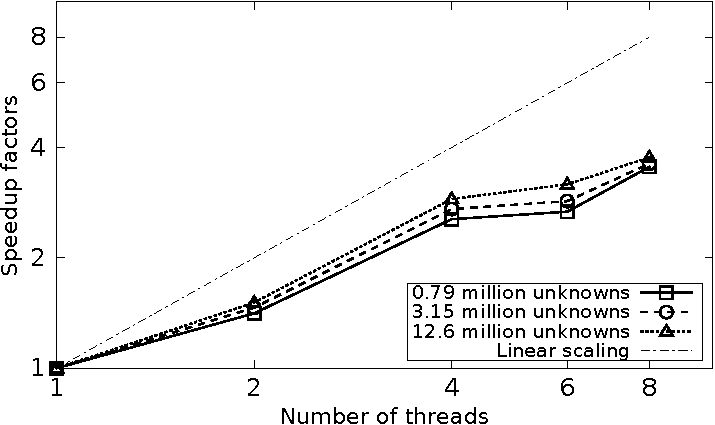
\includegraphics[scale=1.0]{psu} \label{fig:psu_2d}
	}
	\vfill
  %\hspace{+1mm}
	\subfloat[]{
	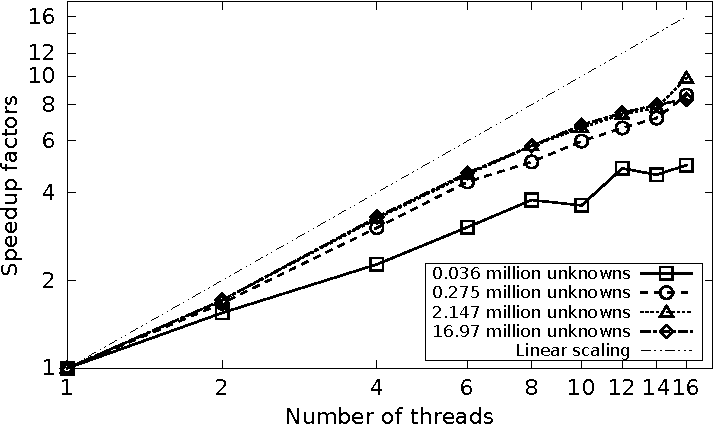
\includegraphics[scale=1.0]{psu_3d} \label{fig:psu_3d}
	}
	}
	\caption[The \acrshort{acr:fmgabp} speedup factors for the 2D and 3D problems.]{\protect\subref*{fig:psu_2d}~The \acrshort{acr:fmgabp} speedup factors for the 2D \gls{acr:ssc} problem on $2\times$quadcore processors node. \protect\subref*{fig:psu_3d}~The \acrshort{acr:fmgabp} speedup factors for the 3D Helmholtz problem on $2\times$8-core processors node.}
	\label{fig:psu}
\end{figure}



To address problems of larger scale, the use of multi-node clusters is required.
For such implementations, the \gls{acr:mpi} programming model is typically used along with sophisticated partitioning algorithms.
Implementations of \gls{acr:fmgabp} using \gls{acr:mpi} are proposed as a future research direction.


\subsection{Manycore GPU Performance}

The \gls{acr:fmgabp} is implemented on an {NVIDIA} Tesla {C2075} for the 2D Helmhotlz problem, as previously defined in \secRef{sec:fgabpVer}, with the number of unknowns ranging from 26K to 4.1M.
Larger problems should be executed on a cluster of \glspl{acr:gpu} because of the \gls{acr:gpu}'s global memory size limits. 
\figRef{fig:gpuRes} shows the speedup achieved by implementing \gls{acr:fmgabp} on a single \gls{acr:gpu} versus the proposed parallel CPU implementation of the method on the SciNet Sandybride cluster node \cite{bib:scinet}.
The SciNet node contains 2$\times$8-core Xeon 2.0~GHz CPUs with 64~\gls{acr:gb} \gls{acr:dram}.
The speedup scalability is also presented in the figure by altering the number of threads for the CPU runs. 
As shown in the figure, the Tesla C2075 outperforms the CPU with up to 12 cores for all problem sizes. 
Larger problems are able to utilize the GPU resources more efficiently thus the GPU is faster than the 16-core CPU node for the largest problem with 4.1M unknowns.
The only case where the GPU did not demonstrate speedups were for the smaller problem sizes (26K and 1M unknowns). 
The average (speedup over all problem sizes) achieved from the GPU implementation compared to the dual-core, quad-core and 12-core CPU settings are 4.8$\times$, 2.3$\times$ and 1.5$\times$ respectively.

\begin{figure}[t]
	\centering{
	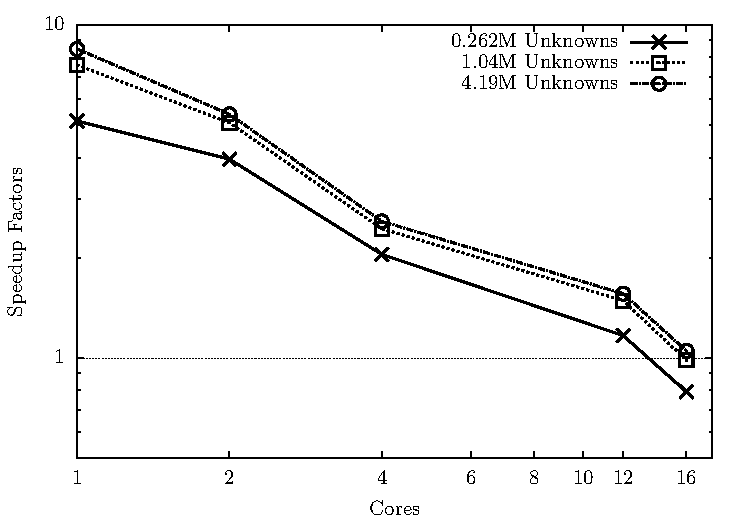
\includegraphics[scale=1.0]{plot_gpu_su.pdf}
	}
	\caption[The FMGaBP GPU implementation speedups.]{The speedup achieved from accelerating FMGaBP on NVIDIA Tesla C2075 compared to the parallel implementation of the method on 1-16 CPU cores.}
	\label{fig:gpuRes}
\end{figure}

\section{Conclusion}
The novel \gls{acr:fmgabp} algorithm was introduced and was shown to achieve high parallel performance due to its matrix-free approach and localized computations.
In addition, we showed for a benchmark Laplace problem that the \gls{acr:fmgabp} algorithm requires less iterations than the \gls{acr:mgpcg} solver.
The threaded multicore implementation of \gls{acr:fmgabp} demonstrates speedups of up to 2.9$\times$ over \libName{deal.II}'s implementation of \gls{acr:mgpcg}.
The GPU implementation showed considerable speedups over the multithreaded CPU implementation.






%==========
\graphicspath{{figs/Chp-Fut/}}
\chapter{Future Directions}
\label{chp:FD}

%%Fakesection Chapter abstract
The \gls{acr:fgabp} and the \gls{acr:fmgabp} algorithms are newly developed solvers that were implemented with only one purpose in mind, which is to efficiently accelerate the \gls{acr:fem} problem and demonstrate high parallel scalability.
Therefore, there may be many possibilities to advance the new algorithms just by looking at the wealth of literature developed in the field of numerical methods in the past decades.
One would find a multitude of methods used to improve the efficiency and the robustness of conventional solvers which could also be applicable here.
In this chapter we survey some of these ideas and discuss their applicability to the new algorithms, as well as the challenges that may be encountered.


\section{Krylov-Subspace Method Preconditioners}

For certain applications, the \gls{acr:fmgabp} algorithm can be very efficient in achieving high convergence; however, many solvers including multigrid can be used as preconditioners in order to improve their robustness especially for complicated applications.
In using the \gls{acr:fmgabp} or the \gls{acr:fgabp} as a preconditioner, one would be interested in obtaining a robust and efficient convergence rate and, most importantly, increasing the parallel scalability of the conventional \acrfullpl{acr:ksm}.
By observing \algRef{alg:pcg}, which is presenting the \gls{acr:pcg} solver, we can see that the preconditioner step can be implemented by either the \gls{acr:fgabp} or the \gls{acr:fmgabp}.
If the \gls{acr:fmgabp} is used, the fast convergence rate should be expected.
In each \gls{acr:pcg} iteration, the residual is used as the right hand side of the preconditioner system.
This can be accomplished by distributing the global residual vector among the \glspl{acr:fn} as local source vectors.
It is important to note here that this distribution of the residual vector to the \glspl{acr:fn} may not be unique.
For example, one choice is to consider to distribute the residual vector elements evenly to all \glspl{acr:fn} connected to that residual element.
Another approach would be to use the $\alpha$ messages as weighting factors, since after each consistent \gls{acr:fgabp} iteration the sum of each \gls{acr:vn} edge $\alpha$ messages is equal to the nodal $\alpha$ sum as expressed by the update rule \eqnRef{eqn:vnaSum}.
The $\beta$ messages are then reinitialized from zero for each \gls{acr:pcg} iteration.
Note that the $\alpha$ messages need not be reinitialized each \gls{acr:pcg} iteration since they do not depend on the right hand side, or the \glspl{acr:fn} source vectors, and their computation can progressively advance each PCG iteration without being restarted.
The \gls{acr:fgabp}, or the \gls{acr:fmgabp}, will then be allowed to iterate a number of times based on the desired preconditioning recipe.


A difficulty may arise in how to compute the \gls{acr:smvm} operation efficiently as in Step~2 of \algRef{alg:pcg}.
In this setting we can still avoid assembling the sparse matrix $A$.
The effect of the \gls{acr:smvm} operation can be obtained by operating on the \glspl{acr:fgabp} data-structure directly.
In other words, we reuse the \gls{acr:fgabp} data-structure for both the \glspl{acr:smvm} and the precondition operations.
The unknown vector would be distributed to the \glspl{acr:fn}, and then each \gls{acr:fn} will perform a local dense matrix vector multiplications using its local characteristic matrix and source vector.
The local results are then gathered using the local to global index information in order to produce the global residual vector.
This \gls{acr:smvm} parallel operation can be performed in a thread-safe manner when element coloring is used.

\section{FMGaBP for Adaptive Refinement}

The \gls{acr:fmgabp} algorithm demonstrated high computational parallel efficiency compared to state-of-the-art solvers; however, the \gls{acr:fmgabp} algorithm was developed based on global mesh refinement, which can result in unnecessary computations when the local \gls{acr:fem} solution accuracy is considered.
The \gls{acr:fmgabp} formulation can be extended to supporting adaptive \glspl{acr:fem} refinement by exploiting the local information already present within the \glspl{acr:fn}.
The resulting adaptive \gls{acr:fmgabp} algorithm would exhibits distributed computations and high parallel efficiency for increasing \gls{acr:fem} solution accuracy.


If the adaptive mesh refinement scheme produces conformal meshes, then the \gls{acr:fmgabp} algorithm can readily be used.
However, if the adaptive mesh refinement scheme produces level meshes that contain hanging-nodes, then the \gls{acr:fmgabp} algorithm would require some reformulation to address this case.
This scheme of adaptive meshing results in special nodes located at the interface between the refined and the non-refined patches of the mesh.
Such nodes are referred to as hanging nodes.
Hanging nodes are termed so because they belong to one side of the mesh, which is the refined side.
In other words, they have the associated basis functions on one side and have none on the other.
The library \libName{deal.II} uses adaptive mesh refinement with hanging-nodes for quadrilateral and hexahedral meshes.
The approach used by \libName{deal.II} involves introducing constraints that ensures the \glspl{acr:fem} solution's continuity across the hanging nodes \cite{bib:janssen2011adaptive}. 
The \gls{acr:fmgabp} can incorporate similar constraints by applying them on a per \gls{acr:fn} basis similar to the defined local belief system as in \eqnRef{eqn:gaussFB}.


\section{FMGaBP MPI Implementation}

In \chpRef{chp:FMGaBP} the \gls{acr:fmgabp} algorithm was scaled for large \gls{acr:fem} problems where the number of elements reaches millions, which is limited only by the memory capacity of the multicore node.
However, for very large scale \gls{acr:fem} simulations involving billions of unknowns the use of clusters of CPU nodes connected by a network is needed. 
Each node in the cluster contains a multicore CPU and its own memory space which can be accessed by each of the CPU cores as shared memory.
Accessing data from one node to another however, has to go through the network which incurs high latency delays.
The \gls{acr:fmgabp} algorithm, due to its high parallel efficiency, demonstrated great performance when executed within one multicore node.
It is also expected that the \gls{acr:fmgabp} can demonstrate even more competitive performance when executed on cluster \gls{acr:hpc} systems, given that a good partitioning algorithm is used to distribute the \glspl{acr:fem} problem across the nodes efficiently.


Cluster \gls{acr:hpc} systems are very scalable and can handle \gls{acr:fmgabp} problems in the order of billions of unknowns.
Obtaining linear scaling on these systems however is very challenging due to its dependence on problem partitioning schemes that impacts memory communication and load-balancing.
Specialized open-source libraries such as \libName{ParMETIS} \cite{bib:parmetis2013} and {P4EST} \cite{bib:p4est} can be used to efficiently partition the
problem.
These libraries can be integrated within the \gls{acr:fgabp} algorithm in order to enhance its message communication pattern.
The \gls{acr:fgabp} software can utilize a hybrid model of multithreading and \gls{acr:mpi} \cite{bib:mpiForum} in order to target the cluster of multicore CPUs.
The multithreading features will enable the \gls{acr:fgabp} software to efficiently exploit parallelism within the multicore node while the
\gls{acr:mpi} interface will exploit parallelism between different nodes.




%==========

%%Fakesection Appendices
%==========
\appendix

%==========
%\include{App-diffCal}
%==========
\graphicspath{{figs/App-GaDiss/}}
\chapter{Gaussian Probability Distribution Functions}
\label{app:gaDiss}

\section{Univariate Gaussian Distribution}

A random variable $u$ that assumes values $u_o$ drawn from a Gaussian distribution $G(\mu,\sigma)$ is referred to as a Gaussian random variable and is denoted as $u \sim G(\mu,\sigma)$.
The univariate Gaussian distribution $G(\mu,\sigma)$, also referred to as the normal distribution, is defined as:
\begin{equation}
	G(u\,;\,\mu,\sigma) \triangleq \frac{1}{\sqrt{2\pi\sigma^2}} \exp\left[-\frac{1}{2\sigma^2}(u-\mu)^2\right]
	\label{eqn:gassDisUnivar}
\end{equation}
where $\mu$ and $\sigma^2$ are referred  as the mean and the variance of the Gaussian distribution correspondingly, while $\sigma$ is referred to as the standard deviation.
The term $1/\sqrt{2\pi\sigma^2}$ is the normalization constant that ensures the property $\int_{-\infty}^{\infty} G(u\,;\,\mu,\sigma)\, \mathrm{d}u = 1$.
As a result, the Gaussian distributions, in their basic form, are fully characterized by their mean and variance parameters.
\figRef{fig:gauPlot} illustrates different Gaussian distribution plots for different $\mu$ and $\sigma$ parameters.
Notice that the Gaussian distribution has a maximum value at its mean point $u=\mu$.
\begin{figure}
	\centering{
	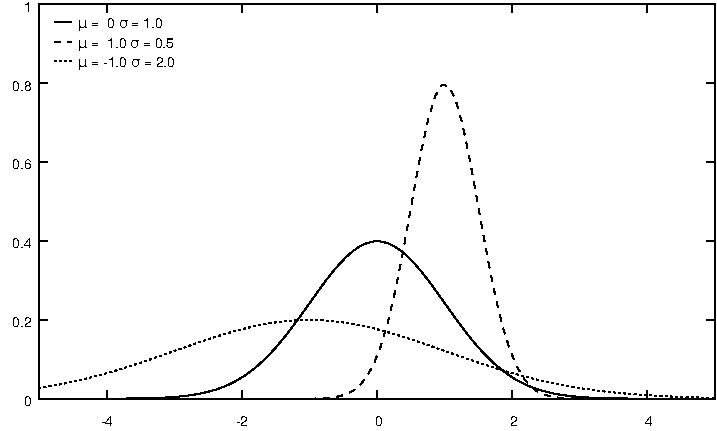
\includegraphics[scale=1.0]{gauPlot}
	}
	\caption[Sample univariate Gaussian distribution plots.]{Sample univariate Gaussian distribution plots for different $\mu$ and $\sigma$ values.}
	\label{fig:gauPlot}
\end{figure}


The Gaussian distribution used in the derivation of the \gls{acr:fgabp} algorithm in \secRef{chp:FGaBP} can more conveniently be represented using a parameterization referred to as the canonical parameterization, or the information form.
The Gaussian distribution can also be used in an un-normalized form by ignoring the normalizing constant.
This does not constitute any loss of information since the Gaussian distribution is fully identified by its mean and variance parameters or, correspondingly, the canonical $\beta$ and $\alpha$ parameters.
The un-normalized canonical representation of the univariate Gaussian distribution is defined as:
\begin{equation}
	G(u\,;\,\beta,\alpha) \propto \exp\left[-\frac{1}{2}\alpha u^2 + \beta u\right]
	\label{eqn:gassDisUnivarCan}
\end{equation}
where $\alpha = 1/\sigma^2$ is the reciprocal of the variance, also referred to as the precision; and $\beta = \mu/\sigma^2$ is the second canonical parameter.


\section{Multivariate Gaussian Distribution}

A collection of $n$ random variables $U=(u_1,u_2,\cdots,u_n)$ have a joint Gaussian probability distribution ($U\sim\mathcal{G}(\bar{\mu},\Sigma)$)  defined as:
\begin{equation}
	\mathcal{G}(U\,;\,\bar{\mu},\Sigma) \triangleq \frac{1}{(2\pi)^{n/2}|\Sigma|^{1/2}} \exp\left[-\frac{1}{2}(U-\bar{\mu})^T\Sigma^{-1}(U-\bar{\mu})\right]
	\label{eqn:gausDisMult}
\end{equation}
where $\bar{\mu}$ is the mean vector of size $n$ for the joint Gaussian random variables $U$; $\Sigma$ is the covariance matrix; and $|\cdot|$ is the determinant operator.
The covariance matrix $\Sigma$ must be \acrfull{acr:spd} in order for $\mathcal{G}$ to be a valid Gaussian probability distribution.
\figRef{fig:gauPlot3D} illustrates a sample bivariate Gaussian distribution plot with $\bar{\mu} = (0.5,0.5)$ and $\Sigma=I$, where $I$ is the identity matrix.
A key property of Gaussian distributions is that they hold their maximum value at $U=\bar{\mu}$.
\begin{figure}
	\centering{
	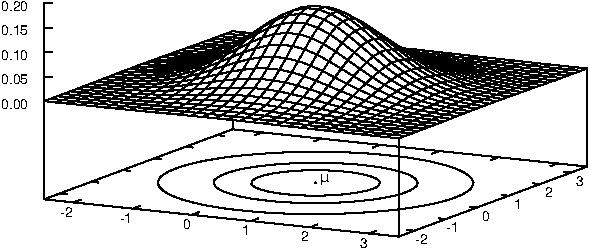
\includegraphics[scale=1.0]{gauPlot3D}
	}
	\caption[Sample bivariate Gaussian distribution plot.]{Sample bivariate Gaussian distribution plot with $\bar{\mu} = (0.5,0.5)$ and $\Sigma=I$.}
	\label{fig:gauPlot3D}
\end{figure}


Similar to the univariate case, the multivariate Gaussian distribution can be represented in the un-normalized canonical form as:
\begin{equation}
	\mathcal{G}(U\,;\,\bar{\mu},\Sigma) \propto \exp\left[-\frac{1}{2}U^T W U + K^T U \right]
	\label{eqn:gausDisMultCan}
\end{equation} 
where $W=\Sigma^{-1}$ is the inverse covariance matrix, also referred to as the precision matrix; and $K=\Sigma^{-1}\bar{\mu}$ is the scaled mean parameter.


The original form of the Gaussian distribution in \eqnRef{eqn:gassDisUnivar} and \eqnRef{eqn:gausDisMult} can be obtained from \eqnRef{eqn:gassDisUnivarCan} and \eqnRef{eqn:gausDisMultCan} correspondingly by completing the algebraic square of the exponent and adjusting the normalizing constant accordingly.
The canonical form is used in the \gls{acr:fgabp} algorithm in order to produce more convenient formulation when multiplying and marginalizing Gaussian distributions as will be illustrated below.


\section{Multiplication of Gaussian Distributions}

Multiplication of any number of Gaussian distributions results in a Gaussian distribution up to a constant.
Using un-normalized canonical forms, the resulting distribution has canonical parameters equal to the sum of the canonical parameters of the multiplied distributions.
The multiplication of $M$ multivariate Gaussian distributions that represent the same Gaussian random variable vector $U$ can be formulated as:
\begin{equation}
	\mathcal{G}(U\,;\,W,K) \propto \prod_{m=1}^{M} \mathcal{G}_m(U\,;\,W_m,K_m)
	\label{eqn:gausDisMultp}
\end{equation}
the resulting distribution $\mathcal{G}$ is Gaussian with canonical parameters computed by:
\begin{align}
	W &= \sum_{m=1}^{M} W_m \\
	K &= \sum_{m=1}^{M} K_m.
\end{align}
This result can readily be applied to scalar Gaussian distributions by replacing the multidimensional parameters with their scalar counterparts.


\section{Marginalization of Gaussian Distributions}

Marginalization of a multivariate Gaussian distribution is integrating away a subset of variables, sometimes referred to as nuisance variables, so that the resulting distribution is a function of the variables of interest.
An important property of Gaussian distributions is that any marginalization of a Gaussian distribution results in a Gaussian distribution.
To further illustrate, suppose that the Gaussian variable vector $U$ is partitioned into two subsets labeled $a$ and $b$ such that $U = (U_a,U_b)$.
Then, to marginalize the Gaussian distribution for $U_a$, we formulate the following:
\begin{equation}
	\mathcal{G}(U_a\,;\,\bar{W_a},\bar{K_a}) \propto \int_{U_b} \mathcal{G}(U\,;\,W,K)\, \mathrm{d}U_b.
	\label{eqn:gausDisMarj}
\end{equation}
To evaluate this integral, we first partition $W$ and $K$ according to the $U_a$ and $U_b$ partitions as follows:
\begin{equation}
	\begin{array}{cc}
		W=\left[%
		\begin{array}{llll}
			W_{aa} & W_{ab} \\
			W_{ba} & W_{bb}
		\end{array}%
		\right],&%
		K=\left[%
		\begin{array}{l}
			K_a \\
			K_b
		\end{array}
		\right].
	\end{array}
	\label{eqn:WKPartitions}
\end{equation}
We then manipulate \eqnRef{eqn:gausDisMarj} by separating the $U_a$ and $U_b$ variables, completing the algebraic square, and using the Gaussian integral identity stated as follows:
\begin{equation}
	\int_U \exp\left[-\frac{1}{2}(U-\mu)^T\Sigma^{-1}(U-\mu)\right]\,\mathrm{d}U = (2\pi)^{n/2}|\Sigma|^{1/2}.
	\label{eqn:GausInteg}
\end{equation}
Finally the integral \eqnRef{eqn:gausDisMarj} is evaluated by finding the $\bar{W_a}$ and $\bar{K_a}$ parameters as follows:
\begin{align}
	\bar{W_a} &= W_{aa} - W_{ab} W_{bb}^{-1} W_{ba}\\
	\bar{K_a} &= K_{a} - W_{ab} W_{bb}^{-1} K_{b}.
	\label{eqn:gausDisMarjWK}
\end{align}

%==========
% \include{App-src}
%==========

%%Fakesection Bibliography
%==========
\begin{singlespace}
	\bibliographystyle{ieeetr}
	\bibliography{IEEEabrv,thesis_phd_yelk_online}
\end{singlespace}
%==========

\end{document}
